\chapterimage{Pictures/chap03/killeroo-control-684x1368.png}
\chapter{形状}\label{chap:形状}
\setcounter{sidenote}{1}

本章中,我们将阐述pbrt对例如球体和三角形等几何图元的抽象。
光线追踪器中对几何形状的仔细抽象是干净系统设计的关键部分,
而且形状是面向对象方法的理想选择。
所有几何图元都实现一个公共接口,
渲染器剩余部分可以使用该接口而无需底层形状的任何细节。
这样能分离pbrt的几何与着色系统。

pbrt将图元的细节隐藏在两层抽象后。
类\refvar{Shape}{}提供对图元原始几何属性的访问,
例如其表面面积和边界框,并且提供光线相交例程。
类\refvar{Primitive}{}封装了关于图元的额外非几何信息,例如其材质属性。
然后渲染器剩余部分只处理\refvar{Primitive}{}抽象接口。
本章将关注只与几何相关的类\refvar{Shape}{};
\refvar{Primitive}{}接口是第\refchap{图元和相交加速}的关键内容。

\section{基本形状接口}\label{sec:基本形状接口}

\refvar{Shape}{}的接口定义于
源文件\href{https://github.com/mmp/pbrt-v3/tree/master/src/core/shape.h}{\ttfamily core/shape.h}中,
\href{https://github.com/mmp/pbrt-v3/tree/master/src/core/shape.cpp}{\ttfamily core/shape.cpp}中
可以找到\refvar{Shape}{}公共方法的定义。
基类\refvar{Shape}{}定义了通用形状接口。
它也暴露了一些对所有\refvar{Shape}{}实现有用的公有数据成员。
\begin{lstlisting}
`\initcode{Shape Declarations}{=}`
class `\initvar{Shape}{}` {
public:
`\refcode{Shape Interface}{}`
`\refcode{Shape Public Data}{}`
};
\end{lstlisting}

所有形状都定义在物体的坐标空间中;
例如,所有球体都定义在球心位于原点的坐标系统中。
为了在场景别处放置球体,必须提供描述从物体空间到世界空间映射的变换。
类\refvar{Shape}{}保存了该变换及其逆。

\refvar{Shape}{}也接收一个布尔参数\refvar{reverseOrientation}{}来
表示其曲面法线方向是否与默认的相反。
该能力很有用,因为曲面法线的朝向用于决定形状哪一面是“外面”。
例如,发光形状只在曲面法线所在那侧是发光的。
该参数值通过pbrt输入文件中的{\ttfamily ReverseOrientation}语句控制。

\refvar{Shape}{}还保存了调用\refvar[SwapsHandedness]{Transform::SwapsHandedness}{()}
来进行物体到世界变换的返回值。
每次找到光线相交处就调用的\refvar{SurfaceInteraction}{}构造函数需要该值,
所以\refvar{Shape}{}构造函数一次性计算并保存它。
\begin{lstlisting}
`\initcode{Shape Method Definitions}{=}\initnext{ShapeMethodDefinitions}`
`\refvar{Shape}{}`::`\refvar{Shape}{}`(const `\refvar{Transform}{}` *ObjectToWorld,
        const `\refvar{Transform}{}` *WorldToObject, bool reverseOrientation)
    : `\refvar{ObjectToWorld}{}`(ObjectToWorld), `\refvar{WorldToObject}{}`(WorldToObject),
      `\refvar{reverseOrientation}{}`(reverseOrientation),
      `\refvar{transformSwapsHandedness}{}`(ObjectToWorld->`\refvar{SwapsHandedness}{}`()) {
}
\end{lstlisting}

一个重要细节是形状保存了指向其变换的指针而不是直接保存\refvar{Transform}{}
对象。回想\refsec{变换}\refvar{Transform}{}对象由总共32个浮点数表示,需要128字节内存;
因为场景中许多形状经常被施加同样的变换,
pbrt维持了一个\refvar{Transform}{}池使它们可以复用,
并把指向共享\refvar{Transform}{}的指针传给形状。
这样,\refvar{Shape}{}析构函数不会删除其\refvar{Transform}{}指针,
而是让\refvar{Transform}{}控制代码来管理那些内存。
\begin{lstlisting}
`\initcode{Shape Public Data}{=}`
const `\refvar{Transform}{}` *`\initvar{ObjectToWorld}{}`, *`\initvar{WorldToObject}{}`;
const bool `\initvar{reverseOrientation}{}`;
const bool `\initvar{transformSwapsHandedness}{}`;
\end{lstlisting}

\subsection{边界}\label{sub:边界}
pbrt要渲染的场景中经常包含处理计算量极大的物体。
对于许多操作,有一个3D\keyindex{包围盒}{bounding volume}{}来封住物体常常很有用。
例如,如果一条光线没有穿过某个包围盒,对于该光线pbrt可以避免处理里面所有物体。

轴对齐边界框是方便的包围盒,因为它们只需要六个浮点值保存且适合很多形状。
而且测试光线与轴对齐边界框相交性的成本极低。
因此每个\refvar{Shape}{}实现必须能
用\refvar{Bounds3f}{}表示的轴对齐边界框包围自己。
有两种不同的包围方法。
第一个是\refvar{ObjectBound}{()},返回在形状的物体空间里的边界框。
\begin{lstlisting}
`\initcode{Shape Interface}{=}\initnext{ShapeInterface}`
virtual `\refvar{Bounds3f}{}` `\initvar{ObjectBound}{}`() const = 0;
\end{lstlisting}

第二个方法是\refvar[Shape::WorldBound]{WorldBound}{()},返回世界空间的边界框。
pbrt提供该方法的默认实现将物体空间边界变换到世界空间。
然而可以轻松计算更紧致的世界空间边界的形状应该重载该方法。
这种形状的一个例子是三角形(\reffig{3.1})。
\begin{figure}[htbp]
    \centering%LaTeX with PSTricks extensions
%%Creator: Inkscape 1.0.1 (3bc2e813f5, 2020-09-07)
%%Please note this file requires PSTricks extensions
\psset{xunit=.5pt,yunit=.5pt,runit=.5pt}
\begin{pspicture}(629.46002197,511.55999756)
{
\newrgbcolor{curcolor}{1 1 1}
\pscustom[linestyle=none,fillstyle=solid,fillcolor=curcolor]
{
\newpath
\moveto(339.26,140.32999756)
\lineto(567.76,140.32999756)
\lineto(567.76,25.82999756)
\closepath
}
}
{
\newrgbcolor{curcolor}{0 0 0}
\pscustom[linewidth=1,linecolor=curcolor]
{
\newpath
\moveto(339.26,140.32999756)
\lineto(567.76,140.32999756)
\lineto(567.76,25.82999756)
\closepath
}
}
{
\newrgbcolor{curcolor}{1 1 1}
\pscustom[linestyle=none,fillstyle=solid,fillcolor=curcolor]
{
\newpath
\moveto(3.48,364.86999756)
\lineto(172.22,210.78999756)
\lineto(95.02,126.23999756)
\closepath
}
}
{
\newrgbcolor{curcolor}{0 0 0}
\pscustom[linewidth=1,linecolor=curcolor]
{
\newpath
\moveto(3.48,364.86999756)
\lineto(172.22,210.78999756)
\lineto(95.02,126.23999756)
\closepath
}
}
{
\newrgbcolor{curcolor}{0 0 0}
\pscustom[linewidth=1,linecolor=curcolor,linestyle=dashed,dash=4]
{
\newpath
\moveto(0.5,367.80000305)
\lineto(173.5,367.80000305)
\lineto(173.5,124.80000305)
\lineto(0.5,124.80000305)
\closepath
}
}
{
\newrgbcolor{curcolor}{0 0 0}
\pscustom[linewidth=1,linecolor=curcolor,linestyle=dashed,dash=4]
{
\newpath
\moveto(334.76000977,142.32998657)
\lineto(570.76000977,142.32998657)
\lineto(570.76000977,26.32998657)
\lineto(334.76000977,26.32998657)
\closepath
}
}
{
\newrgbcolor{curcolor}{1 1 1}
\pscustom[linestyle=none,fillstyle=solid,fillcolor=curcolor]
{
\newpath
\moveto(339.88,393.97999756)
\lineto(568.38,393.68999756)
\lineto(568.23,279.18999756)
\closepath
}
}
{
\newrgbcolor{curcolor}{0 0 0}
\pscustom[linewidth=1,linecolor=curcolor]
{
\newpath
\moveto(339.88,393.97999756)
\lineto(568.38,393.68999756)
\lineto(568.23,279.18999756)
\closepath
}
}
{
\newrgbcolor{curcolor}{0.60000002 0.60000002 0.60000002}
\pscustom[linewidth=1,linecolor=curcolor,linestyle=dashed,dash=4]
{
\newpath
\moveto(335.68396305,394.16577219)
\lineto(463.57916173,510.66391876)
\lineto(627.21528669,331.01921773)
\lineto(499.32008801,214.52107116)
\closepath
}
}
{
\newrgbcolor{curcolor}{0 0 0}
\pscustom[linewidth=1,linecolor=curcolor,linestyle=dashed,dash=4]
{
\newpath
\moveto(333.95999146,511.05999756)
\lineto(628.95999146,511.05999756)
\lineto(628.95999146,214.05999756)
\lineto(333.95999146,214.05999756)
\closepath
}
}
{
\newrgbcolor{curcolor}{0 0 0}
\pscustom[linewidth=1,linecolor=curcolor]
{
\newpath
\moveto(208.1499939,162.76998901)
\lineto(291.20001221,124.44000244)
}
}
{
\newrgbcolor{curcolor}{0 0 0}
\pscustom[linestyle=none,fillstyle=solid,fillcolor=curcolor]
{
\newpath
\moveto(284.43,121.49999756)
\lineto(290.61,124.70999756)
\lineto(289.05,131.49999756)
\lineto(298.56,121.04999756)
\closepath
}
}
{
\newrgbcolor{curcolor}{0.65098041 0.65098041 0.65098041}
\pscustom[linestyle=none,fillstyle=solid,fillcolor=curcolor]
{
\newpath
\moveto(286.35,121.93999756)
\lineto(297.36,121.59999756)
\lineto(291.18,124.44999756)
\closepath
}
}
{
\newrgbcolor{curcolor}{0.40000001 0.40000001 0.40000001}
\pscustom[linestyle=none,fillstyle=solid,fillcolor=curcolor]
{
\newpath
\moveto(289.96,129.74999756)
\lineto(297.36,121.59999756)
\lineto(291.18,124.44999756)
\closepath
}
}
{
\newrgbcolor{curcolor}{0 0 0}
\pscustom[linewidth=1,linecolor=curcolor]
{
\newpath
\moveto(207.8500061,308.70999146)
\lineto(290.36999512,340.97999573)
}
}
{
\newrgbcolor{curcolor}{0 0 0}
\pscustom[linestyle=none,fillstyle=solid,fillcolor=curcolor]
{
\newpath
\moveto(287.8,334.05999756)
\lineto(289.76,340.73999756)
\lineto(283.79,344.30999756)
\lineto(297.91,343.92999756)
\closepath
}
}
{
\newrgbcolor{curcolor}{0.65098041 0.65098041 0.65098041}
\pscustom[linestyle=none,fillstyle=solid,fillcolor=curcolor]
{
\newpath
\moveto(288.81,335.74999756)
\lineto(296.69,343.44999756)
\lineto(290.35,340.96999756)
\closepath
}
}
{
\newrgbcolor{curcolor}{0.40000001 0.40000001 0.40000001}
\pscustom[linestyle=none,fillstyle=solid,fillcolor=curcolor]
{
\newpath
\moveto(285.68,343.75999756)
\lineto(296.69,343.44999756)
\lineto(290.35,340.96999756)
\closepath
}
}
{
\newrgbcolor{curcolor}{0 0 0}
\pscustom[linestyle=none,fillstyle=solid,fillcolor=curcolor]
{
\newpath
\moveto(337.81564237,191.32581977)
\lineto(336.02657987,191.32581977)
\curveto(335.10470487,192.38311143)(334.38855904,193.53675727)(333.87814237,194.78675727)
\curveto(333.36772571,196.03675727)(333.11251737,197.44561143)(333.11251737,199.01331977)
\curveto(333.11251737,200.5810281)(333.36772571,201.98988227)(333.87814237,203.23988227)
\curveto(334.38855904,204.48988227)(335.10470487,205.6435281)(336.02657987,206.70081977)
\lineto(337.81564237,206.70081977)
\lineto(337.81564237,206.62269477)
\curveto(337.39376737,206.24248643)(336.99012154,205.80238227)(336.60470487,205.30238227)
\curveto(336.22449654,204.8075906)(335.87032987,204.2294656)(335.54220487,203.56800727)
\curveto(335.22970487,202.92738227)(334.97449654,202.2216531)(334.77657987,201.45081977)
\curveto(334.58387154,200.67998643)(334.48751737,199.86748643)(334.48751737,199.01331977)
\curveto(334.48751737,198.12269477)(334.58126737,197.3075906)(334.76876737,196.56800727)
\curveto(334.96147571,195.82842393)(335.21928821,195.12529893)(335.54220487,194.45863227)
\curveto(335.85470487,193.81800727)(336.21147571,193.23988227)(336.61251737,192.72425727)
\curveto(337.01355904,192.20342393)(337.41460071,191.76331977)(337.81564237,191.40394477)
\closepath
}
}
{
\newrgbcolor{curcolor}{0 0 0}
\pscustom[linestyle=none,fillstyle=solid,fillcolor=curcolor]
{
\newpath
\moveto(347.19064237,194.54456977)
\lineto(345.72970487,194.54456977)
\lineto(345.72970487,195.47425727)
\curveto(345.59949654,195.3857156)(345.42241321,195.2607156)(345.19845487,195.09925727)
\curveto(344.97970487,194.94300727)(344.76616321,194.81800727)(344.55782987,194.72425727)
\curveto(344.31303821,194.6044656)(344.03178821,194.50550727)(343.71407987,194.42738227)
\curveto(343.39637154,194.34404893)(343.02397571,194.30238227)(342.59689237,194.30238227)
\curveto(341.81043404,194.30238227)(341.14376737,194.56279893)(340.59689237,195.08363227)
\curveto(340.05001737,195.6044656)(339.77657987,196.2685281)(339.77657987,197.07581977)
\curveto(339.77657987,197.7372781)(339.91720487,198.27113227)(340.19845487,198.67738227)
\curveto(340.48491321,199.0888406)(340.89116321,199.41175727)(341.41720487,199.64613227)
\curveto(341.94845487,199.88050727)(342.58647571,200.03936143)(343.33126737,200.12269477)
\curveto(344.07605904,200.2060281)(344.87553821,200.2685281)(345.72970487,200.31019477)
\lineto(345.72970487,200.53675727)
\curveto(345.72970487,200.8700906)(345.66980904,201.14613227)(345.55001737,201.36488227)
\curveto(345.43543404,201.58363227)(345.26876737,201.75550727)(345.05001737,201.88050727)
\curveto(344.84168404,202.00029893)(344.59168404,202.0810281)(344.30001737,202.12269477)
\curveto(344.00835071,202.16436143)(343.70366321,202.18519477)(343.38595487,202.18519477)
\curveto(343.00053821,202.18519477)(342.57085071,202.13311143)(342.09689237,202.02894477)
\curveto(341.62293404,201.92998643)(341.13335071,201.7841531)(340.62814237,201.59144477)
\lineto(340.55001737,201.59144477)
\lineto(340.55001737,203.08363227)
\curveto(340.83647571,203.16175727)(341.25053821,203.24769477)(341.79220487,203.34144477)
\curveto(342.33387154,203.43519477)(342.86772571,203.48206977)(343.39376737,203.48206977)
\curveto(344.00835071,203.48206977)(344.54220487,203.42998643)(344.99532987,203.32581977)
\curveto(345.45366321,203.22686143)(345.84949654,203.05498643)(346.18282987,202.81019477)
\curveto(346.51095487,202.57061143)(346.76095487,202.2607156)(346.93282987,201.88050727)
\curveto(347.10470487,201.50029893)(347.19064237,201.02894477)(347.19064237,200.46644477)
\closepath
\moveto(345.72970487,196.69300727)
\lineto(345.72970487,199.12269477)
\curveto(345.28178821,199.0966531)(344.75314237,199.0575906)(344.14376737,199.00550727)
\curveto(343.53960071,198.95342393)(343.06043404,198.8779031)(342.70626737,198.77894477)
\curveto(342.28439237,198.6591531)(341.94324654,198.4716531)(341.68282987,198.21644477)
\curveto(341.42241321,197.96644477)(341.29220487,197.6200906)(341.29220487,197.17738227)
\curveto(341.29220487,196.67738227)(341.44324654,196.2997781)(341.74532987,196.04456977)
\curveto(342.04741321,195.79456977)(342.50835071,195.66956977)(343.12814237,195.66956977)
\curveto(343.64376737,195.66956977)(344.11512154,195.7685281)(344.54220487,195.96644477)
\curveto(344.96928821,196.16956977)(345.36512154,196.41175727)(345.72970487,196.69300727)
\closepath
}
}
{
\newrgbcolor{curcolor}{0 0 0}
\pscustom[linestyle=none,fillstyle=solid,fillcolor=curcolor]
{
\newpath
\moveto(354.42501737,199.01331977)
\curveto(354.42501737,197.44561143)(354.16980904,196.03675727)(353.65939237,194.78675727)
\curveto(353.14897571,193.53675727)(352.43282987,192.38311143)(351.51095487,191.32581977)
\lineto(349.72189237,191.32581977)
\lineto(349.72189237,191.40394477)
\curveto(350.12293404,191.76331977)(350.52397571,192.20342393)(350.92501737,192.72425727)
\curveto(351.33126737,193.23988227)(351.68803821,193.81800727)(351.99532987,194.45863227)
\curveto(352.31824654,195.12529893)(352.57345487,195.82842393)(352.76095487,196.56800727)
\curveto(352.95366321,197.3075906)(353.05001737,198.12269477)(353.05001737,199.01331977)
\curveto(353.05001737,199.86748643)(352.95366321,200.67998643)(352.76095487,201.45081977)
\curveto(352.56824654,202.2216531)(352.31303821,202.92738227)(351.99532987,203.56800727)
\curveto(351.66720487,204.2294656)(351.31043404,204.8075906)(350.92501737,205.30238227)
\curveto(350.54480904,205.80238227)(350.14376737,206.24248643)(349.72189237,206.62269477)
\lineto(349.72189237,206.70081977)
\lineto(351.51095487,206.70081977)
\curveto(352.43282987,205.6435281)(353.14897571,204.48988227)(353.65939237,203.23988227)
\curveto(354.16980904,201.98988227)(354.42501737,200.5810281)(354.42501737,199.01331977)
\closepath
}
}
{
\newrgbcolor{curcolor}{0 0 0}
\pscustom[linestyle=none,fillstyle=solid,fillcolor=curcolor]
{
\newpath
\moveto(338.77179538,5.00714437)
\lineto(336.98273288,5.00714437)
\curveto(336.06085788,6.06443603)(335.34471204,7.21808187)(334.83429538,8.46808187)
\curveto(334.32387871,9.71808187)(334.06867038,11.12693603)(334.06867038,12.69464437)
\curveto(334.06867038,14.2623527)(334.32387871,15.67120687)(334.83429538,16.92120687)
\curveto(335.34471204,18.17120687)(336.06085788,19.3248527)(336.98273288,20.38214437)
\lineto(338.77179538,20.38214437)
\lineto(338.77179538,20.30401937)
\curveto(338.34992038,19.92381103)(337.94627454,19.48370687)(337.56085788,18.98370687)
\curveto(337.18064954,18.4889152)(336.82648288,17.9107902)(336.49835788,17.24933187)
\curveto(336.18585788,16.60870687)(335.93064954,15.9029777)(335.73273288,15.13214437)
\curveto(335.54002454,14.36131103)(335.44367038,13.54881103)(335.44367038,12.69464437)
\curveto(335.44367038,11.80401937)(335.53742038,10.9889152)(335.72492038,10.24933187)
\curveto(335.91762871,9.50974853)(336.17544121,8.80662353)(336.49835788,8.13995687)
\curveto(336.81085788,7.49933187)(337.16762871,6.92120687)(337.56867038,6.40558187)
\curveto(337.96971204,5.88474853)(338.37075371,5.44464437)(338.77179538,5.08526937)
\closepath
}
}
{
\newrgbcolor{curcolor}{0 0 0}
\pscustom[linestyle=none,fillstyle=solid,fillcolor=curcolor]
{
\newpath
\moveto(349.04523288,12.65558187)
\curveto(349.04523288,11.9264152)(348.94106621,11.2701652)(348.73273288,10.68683187)
\curveto(348.52960788,10.10349853)(348.25356621,9.6139152)(347.90460788,9.21808187)
\curveto(347.53481621,8.80662353)(347.12856621,8.4967277)(346.68585788,8.28839437)
\curveto(346.24314954,8.08526937)(345.75617038,7.98370687)(345.22492038,7.98370687)
\curveto(344.73012871,7.98370687)(344.29783704,8.0436027)(343.92804538,8.16339437)
\curveto(343.55825371,8.2779777)(343.19367038,8.4342277)(342.83429538,8.63214437)
\lineto(342.74054538,8.22589437)
\lineto(341.36554538,8.22589437)
\lineto(341.36554538,20.38214437)
\lineto(342.83429538,20.38214437)
\lineto(342.83429538,16.03839437)
\curveto(343.24575371,16.37693603)(343.68325371,16.6529777)(344.14679538,16.86651937)
\curveto(344.61033704,17.08526937)(345.13117038,17.19464437)(345.70929538,17.19464437)
\curveto(346.74054538,17.19464437)(347.55304538,16.79881103)(348.14679538,16.00714437)
\curveto(348.74575371,15.2154777)(349.04523288,14.0982902)(349.04523288,12.65558187)
\closepath
\moveto(347.52960788,12.61651937)
\curveto(347.52960788,13.65818603)(347.35773288,14.44724853)(347.01398288,14.98370687)
\curveto(346.67023288,15.52537353)(346.11554538,15.79620687)(345.34992038,15.79620687)
\curveto(344.92283704,15.79620687)(344.49054538,15.70245687)(344.05304538,15.51495687)
\curveto(343.61554538,15.3326652)(343.20929538,15.09568603)(342.83429538,14.80401937)
\lineto(342.83429538,9.80401937)
\curveto(343.25096204,9.61651937)(343.60773288,9.48631103)(343.90460788,9.41339437)
\curveto(344.20669121,9.3404777)(344.54783704,9.30401937)(344.92804538,9.30401937)
\curveto(345.74054538,9.30401937)(346.37596204,9.56964437)(346.83429538,10.10089437)
\curveto(347.29783704,10.6373527)(347.52960788,11.47589437)(347.52960788,12.61651937)
\closepath
}
}
{
\newrgbcolor{curcolor}{0 0 0}
\pscustom[linestyle=none,fillstyle=solid,fillcolor=curcolor]
{
\newpath
\moveto(355.74054538,12.69464437)
\curveto(355.74054538,11.12693603)(355.48533704,9.71808187)(354.97492038,8.46808187)
\curveto(354.46450371,7.21808187)(353.74835788,6.06443603)(352.82648288,5.00714437)
\lineto(351.03742038,5.00714437)
\lineto(351.03742038,5.08526937)
\curveto(351.43846204,5.44464437)(351.83950371,5.88474853)(352.24054538,6.40558187)
\curveto(352.64679538,6.92120687)(353.00356621,7.49933187)(353.31085788,8.13995687)
\curveto(353.63377454,8.80662353)(353.88898288,9.50974853)(354.07648288,10.24933187)
\curveto(354.26919121,10.9889152)(354.36554538,11.80401937)(354.36554538,12.69464437)
\curveto(354.36554538,13.54881103)(354.26919121,14.36131103)(354.07648288,15.13214437)
\curveto(353.88377454,15.9029777)(353.62856621,16.60870687)(353.31085788,17.24933187)
\curveto(352.98273288,17.9107902)(352.62596204,18.4889152)(352.24054538,18.98370687)
\curveto(351.86033704,19.48370687)(351.45929538,19.92381103)(351.03742038,20.30401937)
\lineto(351.03742038,20.38214437)
\lineto(352.82648288,20.38214437)
\curveto(353.74835788,19.3248527)(354.46450371,18.17120687)(354.97492038,16.92120687)
\curveto(355.48533704,15.67120687)(355.74054538,14.2623527)(355.74054538,12.69464437)
\closepath
}
}
\end{pspicture}

    \caption{(a)三角形的世界空间边界框通过将其物体空间边界框
        变换到世界空间再寻找包围结果边界框的边界框算得;可能得到肥大的边界框。
        (b)然而,如果三角形的顶点首先从物体空间变换到世界空间再包围,边界框可能合适得多。}
    \label{fig:3.1}
\end{figure}

\begin{lstlisting}
`\refcode{Shape Method Definitions}{+=}\lastnext{ShapeMethodDefinitions}`
`\refvar{Bounds3f}{}` `\refvar{Shape}{}`::`\initvar[Shape::WorldBound]{WorldBound}{}`() const {
    return (*`\refvar{ObjectToWorld}{}`)(`\refvar{ObjectBound}{}`());
}
\end{lstlisting}

\subsection{光线-边界相交}\label{sub:光线-边界相交}
有了\refvar{Bounds3f}{}实例包围形状的用法后,我们将添加一个\refvar{Bounds3}{}方法,即
\refvar{Bounds3::IntersectP}{()},以检查光线-框相交性,
并且如果有的话还返回相交处的两个参数$t$值。

认识边界框的一种方式是将其看作三块厚板\sidenote{译者注:原文slab。}的交集,
每一块是两平行平面之间的空间区域。
为了求光线与框的相交性,我们让光线依次与框的三块厚板相交。
因为厚板与三个坐标轴对齐,在光线-厚板相交中可以应用大量优化。

基本的光线-边界框相交算法算法工作如下:
我们从一个参数化区间开始,它沿我们想要求交的光线覆盖了位置$t$的范围;
该范围通常是$(0,+\infty)$。
然后我们先后计算光线与每个厚板相交的两个参数化$t$位置。
我们计算每个厚板相交区间与当前相交区间的交集,
如果我们发现结果区间退化则返回失败。
如果检查完全部三个厚板后区间是非退化的,
我们就有了光线位于框内的参数范围。
\reffig{3.2}{}说明了该过程,
\reffig{3.3}展示了光线与厚板相交的基本几何结构。
\begin{figure}[htb]
    \centering%LaTeX with PSTricks extensions
%%Creator: Inkscape 1.0.1 (3bc2e813f5, 2020-09-07)
%%Please note this file requires PSTricks extensions
\psset{xunit=.35pt,yunit=.35pt,runit=.35pt}
\begin{pspicture}(405.83999634,310.61999512)
{
\newrgbcolor{curcolor}{0 0.44313726 0.73725492}
\pscustom[linewidth=1.5,linecolor=curcolor]
{
\newpath
\moveto(139.65869141,93.92999268)
\lineto(321.72869873,216.02999878)
}
}
{
\newrgbcolor{curcolor}{0.60000002 0.60000002 0.60000002}
\pscustom[linewidth=1,linecolor=curcolor]
{
\newpath
\moveto(105.2986908,310.61999512)
\lineto(105.2986908,21.85998535)
}
}
{
\newrgbcolor{curcolor}{0.60000002 0.60000002 0.60000002}
\pscustom[linewidth=1,linecolor=curcolor]
{
\newpath
\moveto(321.53869629,310.61999512)
\lineto(321.53869629,21.85998535)
}
}
{
\newrgbcolor{curcolor}{0.60000002 0.60000002 0.60000002}
\pscustom[linewidth=1,linecolor=curcolor]
{
\newpath
\moveto(34.41869354,239.12999725)
\lineto(395.06869507,239.12999725)
}
}
{
\newrgbcolor{curcolor}{0.60000002 0.60000002 0.60000002}
\pscustom[linewidth=1,linecolor=curcolor]
{
\newpath
\moveto(34.41869354,93.97000122)
\lineto(395.06869507,93.97000122)
}
}
{
\newrgbcolor{curcolor}{0 0 0}
\pscustom[linestyle=none,fillstyle=solid,fillcolor=curcolor]
{
\newpath
\moveto(109.33870268,70.9099884)
\curveto(109.33870268,74.49167497)(105.00860571,76.28474111)(102.47627785,73.75241325)
\curveto(99.94394999,71.22008539)(101.73701613,66.88998842)(105.3187027,66.88998842)
\curveto(108.90038926,66.88998842)(110.69345541,71.22008539)(108.16112755,73.75241325)
\curveto(105.62879968,76.28474111)(101.29870272,74.49167497)(101.29870272,70.9099884)
\curveto(101.29870272,67.32830184)(105.62879968,65.53523569)(108.16112755,68.06756355)
\curveto(110.69345541,70.59989142)(108.90038926,74.92998838)(105.3187027,74.92998838)
\curveto(101.73701613,74.92998838)(99.94394999,70.59989142)(102.47627785,68.06756355)
\curveto(105.00860571,65.53523569)(109.33870268,67.32830184)(109.33870268,70.9099884)
\closepath
}
}
{
\newrgbcolor{curcolor}{0 0 0}
\pscustom[linestyle=none,fillstyle=solid,fillcolor=curcolor]
{
\newpath
\moveto(143.72869444,94.02999878)
\curveto(143.72869444,97.61168535)(139.39859747,99.40475149)(136.86626961,96.87242363)
\curveto(134.33394175,94.34009576)(136.12700789,90.0099988)(139.70869446,90.0099988)
\curveto(143.29038102,90.0099988)(145.08344717,94.34009576)(142.55111931,96.87242363)
\curveto(140.01879144,99.40475149)(135.68869448,97.61168535)(135.68869448,94.02999878)
\curveto(135.68869448,90.44831221)(140.01879144,88.65524607)(142.55111931,91.18757393)
\curveto(145.08344717,93.71990179)(143.29038102,98.04999876)(139.70869446,98.04999876)
\curveto(136.12700789,98.04999876)(134.33394175,93.71990179)(136.86626961,91.18757393)
\curveto(139.39859747,88.65524607)(143.72869444,90.44831221)(143.72869444,94.02999878)
\closepath
}
}
{
\newrgbcolor{curcolor}{0 0 0}
\pscustom[linestyle=none,fillstyle=solid,fillcolor=curcolor]
{
\newpath
\moveto(360.25870848,239.1499939)
\curveto(360.25870848,242.73168046)(355.92861151,244.52474661)(353.39628365,241.99241875)
\curveto(350.86395578,239.46009088)(352.65702193,235.12999392)(356.2387085,235.12999392)
\curveto(359.82039506,235.12999392)(361.61346121,239.46009088)(359.08113334,241.99241875)
\curveto(356.54880548,244.52474661)(352.21870852,242.73168046)(352.21870852,239.1499939)
\curveto(352.21870852,235.56830733)(356.54880548,233.77524118)(359.08113334,236.30756905)
\curveto(361.61346121,238.83989691)(359.82039506,243.16999388)(356.2387085,243.16999388)
\curveto(352.65702193,243.16999388)(350.86395578,238.83989691)(353.39628365,236.30756905)
\curveto(355.92861151,233.77524118)(360.25870848,235.56830733)(360.25870848,239.1499939)
\closepath
}
}
{
\newrgbcolor{curcolor}{0 0 0}
\pscustom[linestyle=none,fillstyle=solid,fillcolor=curcolor]
{
\newpath
\moveto(325.53870726,215.86999512)
\curveto(325.53870726,219.45168168)(321.20861029,221.24474783)(318.67628243,218.71241997)
\curveto(316.14395456,216.1800921)(317.93702071,211.84999514)(321.51870728,211.84999514)
\curveto(325.10039384,211.84999514)(326.89345999,216.1800921)(324.36113212,218.71241997)
\curveto(321.82880426,221.24474783)(317.49870729,219.45168168)(317.49870729,215.86999512)
\curveto(317.49870729,212.28830855)(321.82880426,210.49524241)(324.36113212,213.02757027)
\curveto(326.89345999,215.55989813)(325.10039384,219.8899951)(321.51870728,219.8899951)
\curveto(317.93702071,219.8899951)(316.14395456,215.55989813)(318.67628243,213.02757027)
\curveto(321.20861029,210.49524241)(325.53870726,212.28830855)(325.53870726,215.86999512)
\closepath
}
}
{
\newrgbcolor{curcolor}{0 0 0}
\pscustom[linewidth=1,linecolor=curcolor]
{
\newpath
\moveto(349.478695,247.86999512)
\lineto(133.998695,103.35999512)
\lineto(136.498695,99.08999512)
}
}
{
\newrgbcolor{curcolor}{0 0 0}
\pscustom[linewidth=1,linecolor=curcolor]
{
\newpath
\moveto(111.66869354,60.75999451)
\lineto(328.11871338,205.92999268)
}
}
{
\newrgbcolor{curcolor}{0 0 0}
\pscustom[linewidth=1,linecolor=curcolor]
{
\newpath
\moveto(112.248703,60.87998962)
\lineto(108.83869171,65.61000061)
}
}
{
\newrgbcolor{curcolor}{0 0 0}
\pscustom[linewidth=1,linecolor=curcolor]
{
\newpath
\moveto(349.0887146,247.51999664)
\lineto(351.91870117,243.41999817)
}
}
{
\newrgbcolor{curcolor}{0 0 0}
\pscustom[linewidth=1,linecolor=curcolor]
{
\newpath
\moveto(327.75869751,205.61999512)
\lineto(324.72869873,209.94999695)
}
}
{
\newrgbcolor{curcolor}{0 0 0}
\pscustom[linewidth=1.5,linecolor=curcolor]
{
\newpath
\moveto(321.72869873,216.02999878)
\lineto(378.07870483,253.8299942)
}
}
{
\newrgbcolor{curcolor}{0 0 0}
\pscustom[linestyle=none,fillstyle=solid,fillcolor=curcolor]
{
\newpath
\moveto(377.268695,253.28999512)
\lineto(367.368695,256.57999512)
\lineto(388.178695,260.59999512)
\lineto(376.568695,242.86999512)
\closepath
}
}
{
\newrgbcolor{curcolor}{0.65098041 0.65098041 0.65098041}
\pscustom[linestyle=none,fillstyle=solid,fillcolor=curcolor]
{
\newpath
\moveto(386.548695,259.49999512)
\lineto(378.058695,253.80999512)
\lineto(377.498695,245.66999512)
\closepath
}
}
{
\newrgbcolor{curcolor}{0.40000001 0.40000001 0.40000001}
\pscustom[linestyle=none,fillstyle=solid,fillcolor=curcolor]
{
\newpath
\moveto(386.548695,259.49999512)
\lineto(378.058695,253.80999512)
\lineto(370.318695,256.37999512)
\closepath
}
}
{
\newrgbcolor{curcolor}{0 0 0}
\pscustom[linewidth=1.5,linecolor=curcolor]
{
\newpath
\moveto(65.13869476,43.94998169)
\lineto(139.65869141,93.92999268)
}
}
{
\newrgbcolor{curcolor}{0 0 0}
\pscustom[linestyle=none,fillstyle=solid,fillcolor=curcolor]
{
\newpath
\moveto(246.18959279,136.3946905)
\curveto(246.36959279,137.1146905)(247.04459279,139.7696905)(249.02459279,139.7696905)
\curveto(249.15959279,139.7696905)(249.87959279,139.7696905)(250.46459279,139.4096905)
\curveto(249.65459279,139.2296905)(249.11459279,138.5546905)(249.11459279,137.8346905)
\curveto(249.11459279,137.3846905)(249.42959279,136.8446905)(250.19459279,136.8446905)
\curveto(250.82459279,136.8446905)(251.72459279,137.3396905)(251.72459279,138.5096905)
\curveto(251.72459279,139.9946905)(250.05959279,140.3996905)(249.06959279,140.3996905)
\curveto(247.40459279,140.3996905)(246.41459279,138.8696905)(246.05459279,138.2396905)
\curveto(245.33459279,140.1296905)(243.80459279,140.3996905)(242.94959279,140.3996905)
\curveto(239.97959279,140.3996905)(238.31459279,136.7096905)(238.31459279,135.9896905)
\curveto(238.31459279,135.6746905)(238.62959279,135.6746905)(238.67459279,135.6746905)
\curveto(238.89959279,135.6746905)(238.98959279,135.7646905)(239.03459279,135.9896905)
\curveto(240.02459279,139.0496905)(241.91459279,139.7696905)(242.90459279,139.7696905)
\curveto(243.44459279,139.7696905)(244.43459279,139.4996905)(244.43459279,137.8346905)
\curveto(244.43459279,136.9346905)(243.93959279,135.0446905)(242.90459279,130.9946905)
\curveto(242.45459279,129.2396905)(241.41959279,128.0246905)(240.15959279,128.0246905)
\curveto(239.97959279,128.0246905)(239.34959279,128.0246905)(238.71959279,128.3846905)
\curveto(239.43959279,128.5646905)(240.06959279,129.1496905)(240.06959279,129.9596905)
\curveto(240.06959279,130.7246905)(239.43959279,130.9496905)(239.03459279,130.9496905)
\curveto(238.13459279,130.9496905)(237.45959279,130.2296905)(237.45959279,129.2846905)
\curveto(237.45959279,127.9796905)(238.85459279,127.3946905)(240.11459279,127.3946905)
\curveto(242.04959279,127.3946905)(243.08459279,129.4196905)(243.12959279,129.5546905)
\curveto(243.48959279,128.5196905)(244.52459279,127.3946905)(246.23459279,127.3946905)
\curveto(249.20459279,127.3946905)(250.82459279,131.0846905)(250.82459279,131.8046905)
\curveto(250.82459279,132.1196905)(250.59959279,132.1196905)(250.50959279,132.1196905)
\curveto(250.23959279,132.1196905)(250.19459279,131.9846905)(250.10459279,131.8046905)
\curveto(249.15959279,128.6996905)(247.22459279,128.0246905)(246.32459279,128.0246905)
\curveto(245.19959279,128.0246905)(244.74959279,128.9246905)(244.74959279,129.9146905)
\curveto(244.74959279,130.5446905)(244.88459279,131.1746905)(245.19959279,132.4346905)
\closepath
\moveto(246.18959279,136.3946905)
}
}
{
\newrgbcolor{curcolor}{0 0 0}
\pscustom[linestyle=none,fillstyle=solid,fillcolor=curcolor]
{
\newpath
\moveto(102.91989879,14.9150665)
\curveto(103.09989879,15.6350665)(103.77489879,18.2900665)(105.75489879,18.2900665)
\curveto(105.88989879,18.2900665)(106.60989879,18.2900665)(107.19489879,17.9300665)
\curveto(106.38489879,17.7500665)(105.84489879,17.0750665)(105.84489879,16.3550665)
\curveto(105.84489879,15.9050665)(106.15989879,15.3650665)(106.92489879,15.3650665)
\curveto(107.55489879,15.3650665)(108.45489879,15.8600665)(108.45489879,17.0300665)
\curveto(108.45489879,18.5150665)(106.78989879,18.9200665)(105.79989879,18.9200665)
\curveto(104.13489879,18.9200665)(103.14489879,17.3900665)(102.78489879,16.7600665)
\curveto(102.06489879,18.6500665)(100.53489879,18.9200665)(99.67989879,18.9200665)
\curveto(96.70989879,18.9200665)(95.04489879,15.2300665)(95.04489879,14.5100665)
\curveto(95.04489879,14.1950665)(95.35989879,14.1950665)(95.40489879,14.1950665)
\curveto(95.62989879,14.1950665)(95.71989879,14.2850665)(95.76489879,14.5100665)
\curveto(96.75489879,17.5700665)(98.64489879,18.2900665)(99.63489879,18.2900665)
\curveto(100.17489879,18.2900665)(101.16489879,18.0200665)(101.16489879,16.3550665)
\curveto(101.16489879,15.4550665)(100.66989879,13.5650665)(99.63489879,9.5150665)
\curveto(99.18489879,7.7600665)(98.14989879,6.5450665)(96.88989879,6.5450665)
\curveto(96.70989879,6.5450665)(96.07989879,6.5450665)(95.44989879,6.9050665)
\curveto(96.16989879,7.0850665)(96.79989879,7.6700665)(96.79989879,8.4800665)
\curveto(96.79989879,9.2450665)(96.16989879,9.4700665)(95.76489879,9.4700665)
\curveto(94.86489879,9.4700665)(94.18989879,8.7500665)(94.18989879,7.8050665)
\curveto(94.18989879,6.5000665)(95.58489879,5.9150665)(96.84489879,5.9150665)
\curveto(98.77989879,5.9150665)(99.81489879,7.9400665)(99.85989879,8.0750665)
\curveto(100.21989879,7.0400665)(101.25489879,5.9150665)(102.96489879,5.9150665)
\curveto(105.93489879,5.9150665)(107.55489879,9.6050665)(107.55489879,10.3250665)
\curveto(107.55489879,10.6400665)(107.32989879,10.6400665)(107.23989879,10.6400665)
\curveto(106.96989879,10.6400665)(106.92489879,10.5050665)(106.83489879,10.3250665)
\curveto(105.88989879,7.2200665)(103.95489879,6.5450665)(103.05489879,6.5450665)
\curveto(101.92989879,6.5450665)(101.47989879,7.4450665)(101.47989879,8.4350665)
\curveto(101.47989879,9.0650665)(101.61489879,9.6950665)(101.92989879,10.9550665)
\closepath
\moveto(102.91989879,14.9150665)
}
}
{
\newrgbcolor{curcolor}{0 0 0}
\pscustom[linestyle=none,fillstyle=solid,fillcolor=curcolor]
{
\newpath
\moveto(120.08361949,8.31733701)
\curveto(120.08361949,10.52233701)(119.81361949,12.14233701)(118.91361949,13.53733701)
\curveto(118.28361949,14.43733701)(117.02361949,15.24733701)(115.44861949,15.24733701)
\curveto(110.76861949,15.24733701)(110.76861949,9.75733701)(110.76861949,8.31733701)
\curveto(110.76861949,6.87733701)(110.76861949,1.52233701)(115.44861949,1.52233701)
\curveto(120.08361949,1.52233701)(120.08361949,6.87733701)(120.08361949,8.31733701)
\closepath
\moveto(115.44861949,2.10733701)
\curveto(114.50361949,2.10733701)(113.28861949,2.64733701)(112.88361949,4.26733701)
\curveto(112.61361949,5.43733701)(112.61361949,7.10233701)(112.61361949,8.58733701)
\curveto(112.61361949,10.07233701)(112.61361949,11.60233701)(112.88361949,12.68233701)
\curveto(113.33361949,14.25733701)(114.59361949,14.70733701)(115.44861949,14.70733701)
\curveto(116.52861949,14.70733701)(117.56361949,14.03233701)(117.92361949,12.86233701)
\curveto(118.23861949,11.78233701)(118.28361949,10.34233701)(118.28361949,8.58733701)
\curveto(118.28361949,7.10233701)(118.28361949,5.61733701)(118.01361949,4.35733701)
\curveto(117.60861949,2.51233701)(116.25861949,2.10733701)(115.44861949,2.10733701)
\closepath
\moveto(115.44861949,2.10733701)
}
}
{
\newrgbcolor{curcolor}{0 0 0}
\pscustom[linestyle=none,fillstyle=solid,fillcolor=curcolor]
{
\newpath
\moveto(317.55206279,15.4598175)
\curveto(317.73206279,16.1798175)(318.40706279,18.8348175)(320.38706279,18.8348175)
\curveto(320.52206279,18.8348175)(321.24206279,18.8348175)(321.82706279,18.4748175)
\curveto(321.01706279,18.2948175)(320.47706279,17.6198175)(320.47706279,16.8998175)
\curveto(320.47706279,16.4498175)(320.79206279,15.9098175)(321.55706279,15.9098175)
\curveto(322.18706279,15.9098175)(323.08706279,16.4048175)(323.08706279,17.5748175)
\curveto(323.08706279,19.0598175)(321.42206279,19.4648175)(320.43206279,19.4648175)
\curveto(318.76706279,19.4648175)(317.77706279,17.9348175)(317.41706279,17.3048175)
\curveto(316.69706279,19.1948175)(315.16706279,19.4648175)(314.31206279,19.4648175)
\curveto(311.34206279,19.4648175)(309.67706279,15.7748175)(309.67706279,15.0548175)
\curveto(309.67706279,14.7398175)(309.99206279,14.7398175)(310.03706279,14.7398175)
\curveto(310.26206279,14.7398175)(310.35206279,14.8298175)(310.39706279,15.0548175)
\curveto(311.38706279,18.1148175)(313.27706279,18.8348175)(314.26706279,18.8348175)
\curveto(314.80706279,18.8348175)(315.79706279,18.5648175)(315.79706279,16.8998175)
\curveto(315.79706279,15.9998175)(315.30206279,14.1098175)(314.26706279,10.0598175)
\curveto(313.81706279,8.3048175)(312.78206279,7.0898175)(311.52206279,7.0898175)
\curveto(311.34206279,7.0898175)(310.71206279,7.0898175)(310.08206279,7.4498175)
\curveto(310.80206279,7.6298175)(311.43206279,8.2148175)(311.43206279,9.0248175)
\curveto(311.43206279,9.7898175)(310.80206279,10.0148175)(310.39706279,10.0148175)
\curveto(309.49706279,10.0148175)(308.82206279,9.2948175)(308.82206279,8.3498175)
\curveto(308.82206279,7.0448175)(310.21706279,6.4598175)(311.47706279,6.4598175)
\curveto(313.41206279,6.4598175)(314.44706279,8.4848175)(314.49206279,8.6198175)
\curveto(314.85206279,7.5848175)(315.88706279,6.4598175)(317.59706279,6.4598175)
\curveto(320.56706279,6.4598175)(322.18706279,10.1498175)(322.18706279,10.8698175)
\curveto(322.18706279,11.1848175)(321.96206279,11.1848175)(321.87206279,11.1848175)
\curveto(321.60206279,11.1848175)(321.55706279,11.0498175)(321.46706279,10.8698175)
\curveto(320.52206279,7.7648175)(318.58706279,7.0898175)(317.68706279,7.0898175)
\curveto(316.56206279,7.0898175)(316.11206279,7.9898175)(316.11206279,8.9798175)
\curveto(316.11206279,9.6098175)(316.24706279,10.2398175)(316.56206279,11.4998175)
\closepath
\moveto(317.55206279,15.4598175)
}
}
{
\newrgbcolor{curcolor}{0 0 0}
\pscustom[linestyle=none,fillstyle=solid,fillcolor=curcolor]
{
\newpath
\moveto(331.07078349,15.25208801)
\curveto(331.07078349,15.79208801)(331.07078349,15.79208801)(330.48578349,15.79208801)
\curveto(329.18078349,14.53208801)(327.38078349,14.53208801)(326.57078349,14.53208801)
\lineto(326.57078349,13.81208801)
\curveto(327.02078349,13.81208801)(328.37078349,13.81208801)(329.45078349,14.35208801)
\lineto(329.45078349,4.13708801)
\curveto(329.45078349,3.46208801)(329.45078349,3.19208801)(327.47078349,3.19208801)
\lineto(326.70578349,3.19208801)
\lineto(326.70578349,2.47208801)
\curveto(327.06578349,2.47208801)(329.54078349,2.56208801)(330.26078349,2.56208801)
\curveto(330.89078349,2.56208801)(333.41078349,2.47208801)(333.86078349,2.47208801)
\lineto(333.86078349,3.19208801)
\lineto(333.09578349,3.19208801)
\curveto(331.07078349,3.19208801)(331.07078349,3.46208801)(331.07078349,4.13708801)
\closepath
\moveto(331.07078349,15.25208801)
}
}
{
\newrgbcolor{curcolor}{0 0 0}
\pscustom[linestyle=none,fillstyle=solid,fillcolor=curcolor]
{
\newpath
\moveto(23.39313879,245.9607725)
\curveto(23.52813879,246.3657725)(23.52813879,246.4107725)(23.52813879,246.6357725)
\curveto(23.52813879,247.1307725)(23.12313879,247.4007725)(22.67313879,247.4007725)
\curveto(22.40313879,247.4007725)(21.95313879,247.2207725)(21.68313879,246.8157725)
\curveto(21.63813879,246.6357725)(21.36813879,245.7807725)(21.27813879,245.2407725)
\curveto(21.05313879,244.5207725)(20.87313879,243.7107725)(20.69313879,242.9457725)
\lineto(19.38813879,237.7707725)
\curveto(19.29813879,237.3657725)(18.03813879,235.3407725)(16.14813879,235.3407725)
\curveto(14.70813879,235.3407725)(14.39313879,236.6007725)(14.39313879,237.6807725)
\curveto(14.39313879,238.9857725)(14.88813879,240.7857725)(15.83313879,243.3057725)
\curveto(16.28313879,244.4757725)(16.41813879,244.7907725)(16.41813879,245.3757725)
\curveto(16.41813879,246.6357725)(15.51813879,247.7157725)(14.07813879,247.7157725)
\curveto(11.33313879,247.7157725)(10.29813879,243.5307725)(10.29813879,243.3057725)
\curveto(10.29813879,242.9907725)(10.56813879,242.9907725)(10.61313879,242.9907725)
\curveto(10.92813879,242.9907725)(10.92813879,243.0807725)(11.06313879,243.5307725)
\curveto(11.87313879,246.2307725)(12.99813879,247.0857725)(13.98813879,247.0857725)
\curveto(14.21313879,247.0857725)(14.70813879,247.0857725)(14.70813879,246.1857725)
\curveto(14.70813879,245.4657725)(14.39313879,244.7007725)(14.21313879,244.1607725)
\curveto(13.04313879,241.1007725)(12.54813879,239.4807725)(12.54813879,238.1307725)
\curveto(12.54813879,235.5657725)(14.34813879,234.7107725)(16.05813879,234.7107725)
\curveto(17.18313879,234.7107725)(18.12813879,235.2057725)(18.93813879,236.0157725)
\curveto(18.57813879,234.5307725)(18.21813879,233.0907725)(17.09313879,231.5607725)
\curveto(16.32813879,230.6157725)(15.24813879,229.7607725)(13.94313879,229.7607725)
\curveto(13.53813879,229.7607725)(12.23313879,229.8507725)(11.73813879,230.9757725)
\curveto(12.18813879,230.9757725)(12.59313879,230.9757725)(12.95313879,231.3357725)
\curveto(13.26813879,231.5607725)(13.53813879,231.9657725)(13.53813879,232.5057725)
\curveto(13.53813879,233.4057725)(12.77313879,233.4957725)(12.50313879,233.4957725)
\curveto(11.82813879,233.4957725)(10.88313879,233.0457725)(10.88313879,231.6507725)
\curveto(10.88313879,230.2107725)(12.14313879,229.1307725)(13.94313879,229.1307725)
\curveto(16.86813879,229.1307725)(19.83813879,231.7407725)(20.64813879,234.9807725)
\closepath
\moveto(23.39313879,245.9607725)
}
}
{
\newrgbcolor{curcolor}{0 0 0}
\pscustom[linestyle=none,fillstyle=solid,fillcolor=curcolor]
{
\newpath
\moveto(30.21692297,243.50304301)
\curveto(30.21692297,244.04304301)(30.21692297,244.04304301)(29.63192297,244.04304301)
\curveto(28.32692297,242.78304301)(26.52692297,242.78304301)(25.71692297,242.78304301)
\lineto(25.71692297,242.06304301)
\curveto(26.16692297,242.06304301)(27.51692297,242.06304301)(28.59692297,242.60304301)
\lineto(28.59692297,232.38804301)
\curveto(28.59692297,231.71304301)(28.59692297,231.44304301)(26.61692297,231.44304301)
\lineto(25.85192297,231.44304301)
\lineto(25.85192297,230.72304301)
\curveto(26.21192297,230.72304301)(28.68692297,230.81304301)(29.40692297,230.81304301)
\curveto(30.03692297,230.81304301)(32.55692297,230.72304301)(33.00692297,230.72304301)
\lineto(33.00692297,231.44304301)
\lineto(32.24192297,231.44304301)
\curveto(30.21692297,231.44304301)(30.21692297,231.71304301)(30.21692297,232.38804301)
\closepath
\moveto(30.21692297,243.50304301)
}
}
{
\newrgbcolor{curcolor}{0 0 0}
\pscustom[linestyle=none,fillstyle=solid,fillcolor=curcolor]
{
\newpath
\moveto(21.75887879,102.6910795)
\curveto(21.89387879,103.0960795)(21.89387879,103.1410795)(21.89387879,103.3660795)
\curveto(21.89387879,103.8610795)(21.48887879,104.1310795)(21.03887879,104.1310795)
\curveto(20.76887879,104.1310795)(20.31887879,103.9510795)(20.04887879,103.5460795)
\curveto(20.00387879,103.3660795)(19.73387879,102.5110795)(19.64387879,101.9710795)
\curveto(19.41887879,101.2510795)(19.23887879,100.4410795)(19.05887879,99.6760795)
\lineto(17.75387879,94.5010795)
\curveto(17.66387879,94.0960795)(16.40387879,92.0710795)(14.51387879,92.0710795)
\curveto(13.07387879,92.0710795)(12.75887879,93.3310795)(12.75887879,94.4110795)
\curveto(12.75887879,95.7160795)(13.25387879,97.5160795)(14.19887879,100.0360795)
\curveto(14.64887879,101.2060795)(14.78387879,101.5210795)(14.78387879,102.1060795)
\curveto(14.78387879,103.3660795)(13.88387879,104.4460795)(12.44387879,104.4460795)
\curveto(9.69887879,104.4460795)(8.66387879,100.2610795)(8.66387879,100.0360795)
\curveto(8.66387879,99.7210795)(8.93387879,99.7210795)(8.97887879,99.7210795)
\curveto(9.29387879,99.7210795)(9.29387879,99.8110795)(9.42887879,100.2610795)
\curveto(10.23887879,102.9610795)(11.36387879,103.8160795)(12.35387879,103.8160795)
\curveto(12.57887879,103.8160795)(13.07387879,103.8160795)(13.07387879,102.9160795)
\curveto(13.07387879,102.1960795)(12.75887879,101.4310795)(12.57887879,100.8910795)
\curveto(11.40887879,97.8310795)(10.91387879,96.2110795)(10.91387879,94.8610795)
\curveto(10.91387879,92.2960795)(12.71387879,91.4410795)(14.42387879,91.4410795)
\curveto(15.54887879,91.4410795)(16.49387879,91.9360795)(17.30387879,92.7460795)
\curveto(16.94387879,91.2610795)(16.58387879,89.8210795)(15.45887879,88.2910795)
\curveto(14.69387879,87.3460795)(13.61387879,86.4910795)(12.30887879,86.4910795)
\curveto(11.90387879,86.4910795)(10.59887879,86.5810795)(10.10387879,87.7060795)
\curveto(10.55387879,87.7060795)(10.95887879,87.7060795)(11.31887879,88.0660795)
\curveto(11.63387879,88.2910795)(11.90387879,88.6960795)(11.90387879,89.2360795)
\curveto(11.90387879,90.1360795)(11.13887879,90.2260795)(10.86887879,90.2260795)
\curveto(10.19387879,90.2260795)(9.24887879,89.7760795)(9.24887879,88.3810795)
\curveto(9.24887879,86.9410795)(10.50887879,85.8610795)(12.30887879,85.8610795)
\curveto(15.23387879,85.8610795)(18.20387879,88.4710795)(19.01387879,91.7110795)
\closepath
\moveto(21.75887879,102.6910795)
}
}
{
\newrgbcolor{curcolor}{0 0 0}
\pscustom[linestyle=none,fillstyle=solid,fillcolor=curcolor]
{
\newpath
\moveto(32.22766297,93.84335001)
\curveto(32.22766297,96.04835001)(31.95766297,97.66835001)(31.05766297,99.06335001)
\curveto(30.42766297,99.96335001)(29.16766297,100.77335001)(27.59266297,100.77335001)
\curveto(22.91266297,100.77335001)(22.91266297,95.28335001)(22.91266297,93.84335001)
\curveto(22.91266297,92.40335001)(22.91266297,87.04835001)(27.59266297,87.04835001)
\curveto(32.22766297,87.04835001)(32.22766297,92.40335001)(32.22766297,93.84335001)
\closepath
\moveto(27.59266297,87.63335001)
\curveto(26.64766297,87.63335001)(25.43266297,88.17335001)(25.02766297,89.79335001)
\curveto(24.75766297,90.96335001)(24.75766297,92.62835001)(24.75766297,94.11335001)
\curveto(24.75766297,95.59835001)(24.75766297,97.12835001)(25.02766297,98.20835001)
\curveto(25.47766297,99.78335001)(26.73766297,100.23335001)(27.59266297,100.23335001)
\curveto(28.67266297,100.23335001)(29.70766297,99.55835001)(30.06766297,98.38835001)
\curveto(30.38266297,97.30835001)(30.42766297,95.86835001)(30.42766297,94.11335001)
\curveto(30.42766297,92.62835001)(30.42766297,91.14335001)(30.15766297,89.88335001)
\curveto(29.75266297,88.03835001)(28.40266297,87.63335001)(27.59266297,87.63335001)
\closepath
\moveto(27.59266297,87.63335001)
}
}
{
\newrgbcolor{curcolor}{0 0 0}
\pscustom[linestyle=none,fillstyle=solid,fillcolor=curcolor]
{
\newpath
\moveto(228.76452479,184.4038315)
\curveto(228.89952479,184.8088315)(228.89952479,184.8538315)(228.89952479,185.0788315)
\curveto(228.89952479,185.5738315)(228.49452479,185.8438315)(228.04452479,185.8438315)
\curveto(227.77452479,185.8438315)(227.32452479,185.6638315)(227.05452479,185.2588315)
\curveto(227.00952479,185.0788315)(226.73952479,184.2238315)(226.64952479,183.6838315)
\curveto(226.42452479,182.9638315)(226.24452479,182.1538315)(226.06452479,181.3888315)
\lineto(224.75952479,176.2138315)
\curveto(224.66952479,175.8088315)(223.40952479,173.7838315)(221.51952479,173.7838315)
\curveto(220.07952479,173.7838315)(219.76452479,175.0438315)(219.76452479,176.1238315)
\curveto(219.76452479,177.4288315)(220.25952479,179.2288315)(221.20452479,181.7488315)
\curveto(221.65452479,182.9188315)(221.78952479,183.2338315)(221.78952479,183.8188315)
\curveto(221.78952479,185.0788315)(220.88952479,186.1588315)(219.44952479,186.1588315)
\curveto(216.70452479,186.1588315)(215.66952479,181.9738315)(215.66952479,181.7488315)
\curveto(215.66952479,181.4338315)(215.93952479,181.4338315)(215.98452479,181.4338315)
\curveto(216.29952479,181.4338315)(216.29952479,181.5238315)(216.43452479,181.9738315)
\curveto(217.24452479,184.6738315)(218.36952479,185.5288315)(219.35952479,185.5288315)
\curveto(219.58452479,185.5288315)(220.07952479,185.5288315)(220.07952479,184.6288315)
\curveto(220.07952479,183.9088315)(219.76452479,183.1438315)(219.58452479,182.6038315)
\curveto(218.41452479,179.5438315)(217.91952479,177.9238315)(217.91952479,176.5738315)
\curveto(217.91952479,174.0088315)(219.71952479,173.1538315)(221.42952479,173.1538315)
\curveto(222.55452479,173.1538315)(223.49952479,173.6488315)(224.30952479,174.4588315)
\curveto(223.94952479,172.9738315)(223.58952479,171.5338315)(222.46452479,170.0038315)
\curveto(221.69952479,169.0588315)(220.61952479,168.2038315)(219.31452479,168.2038315)
\curveto(218.90952479,168.2038315)(217.60452479,168.2938315)(217.10952479,169.4188315)
\curveto(217.55952479,169.4188315)(217.96452479,169.4188315)(218.32452479,169.7788315)
\curveto(218.63952479,170.0038315)(218.90952479,170.4088315)(218.90952479,170.9488315)
\curveto(218.90952479,171.8488315)(218.14452479,171.9388315)(217.87452479,171.9388315)
\curveto(217.19952479,171.9388315)(216.25452479,171.4888315)(216.25452479,170.0938315)
\curveto(216.25452479,168.6538315)(217.51452479,167.5738315)(219.31452479,167.5738315)
\curveto(222.23952479,167.5738315)(225.20952479,170.1838315)(226.01952479,173.4238315)
\closepath
\moveto(228.76452479,184.4038315)
}
}
\end{pspicture}

    \caption{光线与轴对齐边界框相交。我们依次计算与每个厚板的交点,逐渐缩窄参数区间。
        这里的2D形式中,沿光线与$x$和$y$相交范围(蓝色线段)给出了框中光线的范围。}
    \label{fig:3.2}
\end{figure}
\begin{figure}[htb]
    \centering%LaTeX with PSTricks extensions
%%Creator: Inkscape 1.0.1 (3bc2e813f5, 2020-09-07)
%%Please note this file requires PSTricks extensions
\psset{xunit=.5pt,yunit=.5pt,runit=.5pt}
\begin{pspicture}(428.11999512,309.83999634)
{
\newrgbcolor{curcolor}{0.60000002 0.60000002 0.60000002}
\pscustom[linewidth=1,linecolor=curcolor]
{
\newpath
\moveto(40.58000183,309.83999634)
\lineto(40.58000183,21.07998657)
}
}
{
\newrgbcolor{curcolor}{0.60000002 0.60000002 0.60000002}
\pscustom[linewidth=1,linecolor=curcolor]
{
\newpath
\moveto(256.82000732,309.83999634)
\lineto(256.82000732,21.07998657)
}
}
{
\newrgbcolor{curcolor}{0 0 0}
\pscustom[linewidth=1.5,linecolor=curcolor]
{
\newpath
\moveto(0.41999999,43.16998291)
\lineto(313.35998535,253.04999542)
}
}
{
\newrgbcolor{curcolor}{0 0 0}
\pscustom[linestyle=none,fillstyle=solid,fillcolor=curcolor]
{
\newpath
\moveto(311.84,242.08999634)
\lineto(312.55,252.50999634)
\lineto(302.64,255.79999634)
\lineto(323.45,259.81999634)
\closepath
}
}
{
\newrgbcolor{curcolor}{0.65098041 0.65098041 0.65098041}
\pscustom[linestyle=none,fillstyle=solid,fillcolor=curcolor]
{
\newpath
\moveto(312.78,244.88999634)
\lineto(321.82,258.71999634)
\lineto(313.34,253.02999634)
\closepath
}
}
{
\newrgbcolor{curcolor}{0.40000001 0.40000001 0.40000001}
\pscustom[linestyle=none,fillstyle=solid,fillcolor=curcolor]
{
\newpath
\moveto(305.6,255.59999634)
\lineto(321.82,258.71999634)
\lineto(313.34,253.02999634)
\closepath
}
}
{
\newrgbcolor{curcolor}{0 0 0}
\pscustom[linestyle=none,fillstyle=solid,fillcolor=curcolor]
{
\newpath
\moveto(44.61000013,70.12998962)
\curveto(44.61000013,73.71167619)(40.27990317,75.50474234)(37.7475753,72.97241447)
\curveto(35.21524744,70.44008661)(37.00831359,66.10998964)(40.59000015,66.10998964)
\curveto(44.17168672,66.10998964)(45.96475286,70.44008661)(43.432425,72.97241447)
\curveto(40.90009714,75.50474234)(36.57000017,73.71167619)(36.57000017,70.12998962)
\curveto(36.57000017,66.54830306)(40.90009714,64.75523691)(43.432425,67.28756478)
\curveto(45.96475286,69.81989264)(44.17168672,74.1499896)(40.59000015,74.1499896)
\curveto(37.00831359,74.1499896)(35.21524744,69.81989264)(37.7475753,67.28756478)
\curveto(40.27990317,64.75523691)(44.61000013,66.54830306)(44.61000013,70.12998962)
\closepath
}
}
{
\newrgbcolor{curcolor}{0 0 0}
\pscustom[linestyle=none,fillstyle=solid,fillcolor=curcolor]
{
\newpath
\moveto(260.81998777,215.08999634)
\curveto(260.81998777,218.6716829)(256.48989081,220.46474905)(253.95756294,217.93242119)
\curveto(251.42523508,215.40009332)(253.21830123,211.06999636)(256.79998779,211.06999636)
\curveto(260.38167436,211.06999636)(262.1747405,215.40009332)(259.64241264,217.93242119)
\curveto(257.11008478,220.46474905)(252.77998781,218.6716829)(252.77998781,215.08999634)
\curveto(252.77998781,211.50830977)(257.11008478,209.71524363)(259.64241264,212.24757149)
\curveto(262.1747405,214.77989935)(260.38167436,219.10999632)(256.79998779,219.10999632)
\curveto(253.21830123,219.10999632)(251.42523508,214.77989935)(253.95756294,212.24757149)
\curveto(256.48989081,209.71524363)(260.81998777,211.50830977)(260.81998777,215.08999634)
\closepath
}
}
{
\newrgbcolor{curcolor}{0 0 0}
\pscustom[linewidth=1,linecolor=curcolor]
{
\newpath
\moveto(256.8999939,112.25)
\lineto(338.73001099,112.25)
}
}
{
\newrgbcolor{curcolor}{0 0 0}
\pscustom[linestyle=none,fillstyle=solid,fillcolor=curcolor]
{
\newpath
\moveto(333.82,106.73999634)
\lineto(338.08,112.24999634)
\lineto(333.82,117.74999634)
\lineto(346.83,112.24999634)
\closepath
}
}
{
\newrgbcolor{curcolor}{0.65098041 0.65098041 0.65098041}
\pscustom[linestyle=none,fillstyle=solid,fillcolor=curcolor]
{
\newpath
\moveto(335.38,107.93999634)
\lineto(345.52,112.24999634)
\lineto(338.71,112.24999634)
\closepath
}
}
{
\newrgbcolor{curcolor}{0.40000001 0.40000001 0.40000001}
\pscustom[linestyle=none,fillstyle=solid,fillcolor=curcolor]
{
\newpath
\moveto(335.38,116.53999634)
\lineto(345.52,112.24999634)
\lineto(338.71,112.24999634)
\closepath
}
}
{
\newrgbcolor{curcolor}{0 0 0}
\pscustom[linestyle=none,fillstyle=solid,fillcolor=curcolor]
{
\newpath
\moveto(24.8654161,12.75434146)
\curveto(24.9904161,13.25434146)(25.4591661,15.09809146)(26.8341661,15.09809146)
\curveto(26.9279161,15.09809146)(27.4279161,15.09809146)(27.8341661,14.84809146)
\curveto(27.2716661,14.72309146)(26.8966661,14.25434146)(26.8966661,13.75434146)
\curveto(26.8966661,13.44184146)(27.1154161,13.06684146)(27.6466661,13.06684146)
\curveto(28.0841661,13.06684146)(28.7091661,13.41059146)(28.7091661,14.22309146)
\curveto(28.7091661,15.25434146)(27.5529161,15.53559146)(26.8654161,15.53559146)
\curveto(25.7091661,15.53559146)(25.0216661,14.47309146)(24.7716661,14.03559146)
\curveto(24.2716661,15.34809146)(23.2091661,15.53559146)(22.6154161,15.53559146)
\curveto(20.5529161,15.53559146)(19.3966661,12.97309146)(19.3966661,12.47309146)
\curveto(19.3966661,12.25434146)(19.6154161,12.25434146)(19.6466661,12.25434146)
\curveto(19.8029161,12.25434146)(19.8654161,12.31684146)(19.8966661,12.47309146)
\curveto(20.5841661,14.59809146)(21.8966661,15.09809146)(22.5841661,15.09809146)
\curveto(22.9591661,15.09809146)(23.6466661,14.91059146)(23.6466661,13.75434146)
\curveto(23.6466661,13.12934146)(23.3029161,11.81684146)(22.5841661,9.00434146)
\curveto(22.2716661,7.78559146)(21.5529161,6.94184146)(20.6779161,6.94184146)
\curveto(20.5529161,6.94184146)(20.1154161,6.94184146)(19.6779161,7.19184146)
\curveto(20.1779161,7.31684146)(20.6154161,7.72309146)(20.6154161,8.28559146)
\curveto(20.6154161,8.81684146)(20.1779161,8.97309146)(19.8966661,8.97309146)
\curveto(19.2716661,8.97309146)(18.8029161,8.47309146)(18.8029161,7.81684146)
\curveto(18.8029161,6.91059146)(19.7716661,6.50434146)(20.6466661,6.50434146)
\curveto(21.9904161,6.50434146)(22.7091661,7.91059146)(22.7404161,8.00434146)
\curveto(22.9904161,7.28559146)(23.7091661,6.50434146)(24.8966661,6.50434146)
\curveto(26.9591661,6.50434146)(28.0841661,9.06684146)(28.0841661,9.56684146)
\curveto(28.0841661,9.78559146)(27.9279161,9.78559146)(27.8654161,9.78559146)
\curveto(27.6779161,9.78559146)(27.6466661,9.69184146)(27.5841661,9.56684146)
\curveto(26.9279161,7.41059146)(25.5841661,6.94184146)(24.9591661,6.94184146)
\curveto(24.1779161,6.94184146)(23.8654161,7.56684146)(23.8654161,8.25434146)
\curveto(23.8654161,8.69184146)(23.9591661,9.12934146)(24.1779161,10.00434146)
\closepath
\moveto(24.8654161,12.75434146)
}
}
{
\newrgbcolor{curcolor}{0 0 0}
\pscustom[linestyle=none,fillstyle=solid,fillcolor=curcolor]
{
\newpath
\moveto(48.82066208,13.25434146)
\curveto(49.13316208,13.25434146)(49.50816208,13.25434146)(49.50816208,13.62934146)
\curveto(49.50816208,14.03559146)(49.13316208,14.03559146)(48.85191208,14.03559146)
\lineto(36.91441208,14.03559146)
\curveto(36.63316208,14.03559146)(36.25816208,14.03559146)(36.25816208,13.62934146)
\curveto(36.25816208,13.25434146)(36.63316208,13.25434146)(36.91441208,13.25434146)
\closepath
\moveto(48.85191208,9.37934146)
\curveto(49.13316208,9.37934146)(49.50816208,9.37934146)(49.50816208,9.78559146)
\curveto(49.50816208,10.16059146)(49.13316208,10.16059146)(48.82066208,10.16059146)
\lineto(36.91441208,10.16059146)
\curveto(36.63316208,10.16059146)(36.25816208,10.16059146)(36.25816208,9.78559146)
\curveto(36.25816208,9.37934146)(36.63316208,9.37934146)(36.91441208,9.37934146)
\closepath
\moveto(48.85191208,9.37934146)
}
}
{
\newrgbcolor{curcolor}{0 0 0}
\pscustom[linestyle=none,fillstyle=solid,fillcolor=curcolor]
{
\newpath
\moveto(62.82140976,12.75434146)
\curveto(62.94640976,13.25434146)(63.41515976,15.09809146)(64.79015976,15.09809146)
\curveto(64.88390976,15.09809146)(65.38390976,15.09809146)(65.79015976,14.84809146)
\curveto(65.22765976,14.72309146)(64.85265976,14.25434146)(64.85265976,13.75434146)
\curveto(64.85265976,13.44184146)(65.07140976,13.06684146)(65.60265976,13.06684146)
\curveto(66.04015976,13.06684146)(66.66515976,13.41059146)(66.66515976,14.22309146)
\curveto(66.66515976,15.25434146)(65.50890976,15.53559146)(64.82140976,15.53559146)
\curveto(63.66515976,15.53559146)(62.97765976,14.47309146)(62.72765976,14.03559146)
\curveto(62.22765976,15.34809146)(61.16515976,15.53559146)(60.57140976,15.53559146)
\curveto(58.50890976,15.53559146)(57.35265976,12.97309146)(57.35265976,12.47309146)
\curveto(57.35265976,12.25434146)(57.57140976,12.25434146)(57.60265976,12.25434146)
\curveto(57.75890976,12.25434146)(57.82140976,12.31684146)(57.85265976,12.47309146)
\curveto(58.54015976,14.59809146)(59.85265976,15.09809146)(60.54015976,15.09809146)
\curveto(60.91515976,15.09809146)(61.60265976,14.91059146)(61.60265976,13.75434146)
\curveto(61.60265976,13.12934146)(61.25890976,11.81684146)(60.54015976,9.00434146)
\curveto(60.22765976,7.78559146)(59.50890976,6.94184146)(58.63390976,6.94184146)
\curveto(58.50890976,6.94184146)(58.07140976,6.94184146)(57.63390976,7.19184146)
\curveto(58.13390976,7.31684146)(58.57140976,7.72309146)(58.57140976,8.28559146)
\curveto(58.57140976,8.81684146)(58.13390976,8.97309146)(57.85265976,8.97309146)
\curveto(57.22765976,8.97309146)(56.75890976,8.47309146)(56.75890976,7.81684146)
\curveto(56.75890976,6.91059146)(57.72765976,6.50434146)(58.60265976,6.50434146)
\curveto(59.94640976,6.50434146)(60.66515976,7.91059146)(60.69640976,8.00434146)
\curveto(60.94640976,7.28559146)(61.66515976,6.50434146)(62.85265976,6.50434146)
\curveto(64.91515976,6.50434146)(66.04015976,9.06684146)(66.04015976,9.56684146)
\curveto(66.04015976,9.78559146)(65.88390976,9.78559146)(65.82140976,9.78559146)
\curveto(65.63390976,9.78559146)(65.60265976,9.69184146)(65.54015976,9.56684146)
\curveto(64.88390976,7.41059146)(63.54015976,6.94184146)(62.91515976,6.94184146)
\curveto(62.13390976,6.94184146)(61.82140976,7.56684146)(61.82140976,8.25434146)
\curveto(61.82140976,8.69184146)(61.91515976,9.12934146)(62.13390976,10.00434146)
\closepath
\moveto(62.82140976,12.75434146)
}
}
{
\newrgbcolor{curcolor}{0 0 0}
\pscustom[linestyle=none,fillstyle=solid,fillcolor=curcolor]
{
\newpath
\moveto(74.74066024,8.17258487)
\curveto(74.74066024,9.70383487)(74.55316024,10.82883487)(73.92816024,11.79758487)
\curveto(73.49066024,12.42258487)(72.61566024,12.98508487)(71.52191024,12.98508487)
\curveto(68.27191024,12.98508487)(68.27191024,9.17258487)(68.27191024,8.17258487)
\curveto(68.27191024,7.17258487)(68.27191024,3.45383487)(71.52191024,3.45383487)
\curveto(74.74066024,3.45383487)(74.74066024,7.17258487)(74.74066024,8.17258487)
\closepath
\moveto(71.52191024,3.86008487)
\curveto(70.86566024,3.86008487)(70.02191024,4.23508487)(69.74066024,5.36008487)
\curveto(69.55316024,6.17258487)(69.55316024,7.32883487)(69.55316024,8.36008487)
\curveto(69.55316024,9.39133487)(69.55316024,10.45383487)(69.74066024,11.20383487)
\curveto(70.05316024,12.29758487)(70.92816024,12.61008487)(71.52191024,12.61008487)
\curveto(72.27191024,12.61008487)(72.99066024,12.14133487)(73.24066024,11.32883487)
\curveto(73.45941024,10.57883487)(73.49066024,9.57883487)(73.49066024,8.36008487)
\curveto(73.49066024,7.32883487)(73.49066024,6.29758487)(73.30316024,5.42258487)
\curveto(73.02191024,4.14133487)(72.08441024,3.86008487)(71.52191024,3.86008487)
\closepath
\moveto(71.52191024,3.86008487)
}
}
{
\newrgbcolor{curcolor}{0 0 0}
\pscustom[linestyle=none,fillstyle=solid,fillcolor=curcolor]
{
\newpath
\moveto(237.5895741,13.28483146)
\curveto(237.7145741,13.78483146)(238.1833241,15.62858146)(239.5583241,15.62858146)
\curveto(239.6520741,15.62858146)(240.1520741,15.62858146)(240.5583241,15.37858146)
\curveto(239.9958241,15.25358146)(239.6208241,14.78483146)(239.6208241,14.28483146)
\curveto(239.6208241,13.97233146)(239.8395741,13.59733146)(240.3708241,13.59733146)
\curveto(240.8083241,13.59733146)(241.4333241,13.94108146)(241.4333241,14.75358146)
\curveto(241.4333241,15.78483146)(240.2770741,16.06608146)(239.5895741,16.06608146)
\curveto(238.4333241,16.06608146)(237.7458241,15.00358146)(237.4958241,14.56608146)
\curveto(236.9958241,15.87858146)(235.9333241,16.06608146)(235.3395741,16.06608146)
\curveto(233.2770741,16.06608146)(232.1208241,13.50358146)(232.1208241,13.00358146)
\curveto(232.1208241,12.78483146)(232.3395741,12.78483146)(232.3708241,12.78483146)
\curveto(232.5270741,12.78483146)(232.5895741,12.84733146)(232.6208241,13.00358146)
\curveto(233.3083241,15.12858146)(234.6208241,15.62858146)(235.3083241,15.62858146)
\curveto(235.6833241,15.62858146)(236.3708241,15.44108146)(236.3708241,14.28483146)
\curveto(236.3708241,13.65983146)(236.0270741,12.34733146)(235.3083241,9.53483146)
\curveto(234.9958241,8.31608146)(234.2770741,7.47233146)(233.4020741,7.47233146)
\curveto(233.2770741,7.47233146)(232.8395741,7.47233146)(232.4020741,7.72233146)
\curveto(232.9020741,7.84733146)(233.3395741,8.25358146)(233.3395741,8.81608146)
\curveto(233.3395741,9.34733146)(232.9020741,9.50358146)(232.6208241,9.50358146)
\curveto(231.9958241,9.50358146)(231.5270741,9.00358146)(231.5270741,8.34733146)
\curveto(231.5270741,7.44108146)(232.4958241,7.03483146)(233.3708241,7.03483146)
\curveto(234.7145741,7.03483146)(235.4333241,8.44108146)(235.4645741,8.53483146)
\curveto(235.7145741,7.81608146)(236.4333241,7.03483146)(237.6208241,7.03483146)
\curveto(239.6833241,7.03483146)(240.8083241,9.59733146)(240.8083241,10.09733146)
\curveto(240.8083241,10.31608146)(240.6520741,10.31608146)(240.5895741,10.31608146)
\curveto(240.4020741,10.31608146)(240.3708241,10.22233146)(240.3083241,10.09733146)
\curveto(239.6520741,7.94108146)(238.3083241,7.47233146)(237.6833241,7.47233146)
\curveto(236.9020741,7.47233146)(236.5895741,8.09733146)(236.5895741,8.78483146)
\curveto(236.5895741,9.22233146)(236.6833241,9.65983146)(236.9020741,10.53483146)
\closepath
\moveto(237.5895741,13.28483146)
}
}
{
\newrgbcolor{curcolor}{0 0 0}
\pscustom[linestyle=none,fillstyle=solid,fillcolor=curcolor]
{
\newpath
\moveto(261.54482008,13.78483146)
\curveto(261.85732008,13.78483146)(262.23232008,13.78483146)(262.23232008,14.15983146)
\curveto(262.23232008,14.56608146)(261.85732008,14.56608146)(261.57607008,14.56608146)
\lineto(249.63857008,14.56608146)
\curveto(249.35732008,14.56608146)(248.98232008,14.56608146)(248.98232008,14.15983146)
\curveto(248.98232008,13.78483146)(249.35732008,13.78483146)(249.63857008,13.78483146)
\closepath
\moveto(261.57607008,9.90983146)
\curveto(261.85732008,9.90983146)(262.23232008,9.90983146)(262.23232008,10.31608146)
\curveto(262.23232008,10.69108146)(261.85732008,10.69108146)(261.54482008,10.69108146)
\lineto(249.63857008,10.69108146)
\curveto(249.35732008,10.69108146)(248.98232008,10.69108146)(248.98232008,10.31608146)
\curveto(248.98232008,9.90983146)(249.35732008,9.90983146)(249.63857008,9.90983146)
\closepath
\moveto(261.57607008,9.90983146)
}
}
{
\newrgbcolor{curcolor}{0 0 0}
\pscustom[linestyle=none,fillstyle=solid,fillcolor=curcolor]
{
\newpath
\moveto(275.54556776,13.28483146)
\curveto(275.67056776,13.78483146)(276.13931776,15.62858146)(277.51431776,15.62858146)
\curveto(277.60806776,15.62858146)(278.10806776,15.62858146)(278.51431776,15.37858146)
\curveto(277.95181776,15.25358146)(277.57681776,14.78483146)(277.57681776,14.28483146)
\curveto(277.57681776,13.97233146)(277.79556776,13.59733146)(278.32681776,13.59733146)
\curveto(278.76431776,13.59733146)(279.38931776,13.94108146)(279.38931776,14.75358146)
\curveto(279.38931776,15.78483146)(278.23306776,16.06608146)(277.54556776,16.06608146)
\curveto(276.38931776,16.06608146)(275.70181776,15.00358146)(275.45181776,14.56608146)
\curveto(274.95181776,15.87858146)(273.88931776,16.06608146)(273.29556776,16.06608146)
\curveto(271.23306776,16.06608146)(270.07681776,13.50358146)(270.07681776,13.00358146)
\curveto(270.07681776,12.78483146)(270.29556776,12.78483146)(270.32681776,12.78483146)
\curveto(270.48306776,12.78483146)(270.54556776,12.84733146)(270.57681776,13.00358146)
\curveto(271.26431776,15.12858146)(272.57681776,15.62858146)(273.26431776,15.62858146)
\curveto(273.63931776,15.62858146)(274.32681776,15.44108146)(274.32681776,14.28483146)
\curveto(274.32681776,13.65983146)(273.98306776,12.34733146)(273.26431776,9.53483146)
\curveto(272.95181776,8.31608146)(272.23306776,7.47233146)(271.35806776,7.47233146)
\curveto(271.23306776,7.47233146)(270.79556776,7.47233146)(270.35806776,7.72233146)
\curveto(270.85806776,7.84733146)(271.29556776,8.25358146)(271.29556776,8.81608146)
\curveto(271.29556776,9.34733146)(270.85806776,9.50358146)(270.57681776,9.50358146)
\curveto(269.95181776,9.50358146)(269.48306776,9.00358146)(269.48306776,8.34733146)
\curveto(269.48306776,7.44108146)(270.45181776,7.03483146)(271.32681776,7.03483146)
\curveto(272.67056776,7.03483146)(273.38931776,8.44108146)(273.42056776,8.53483146)
\curveto(273.67056776,7.81608146)(274.38931776,7.03483146)(275.57681776,7.03483146)
\curveto(277.63931776,7.03483146)(278.76431776,9.59733146)(278.76431776,10.09733146)
\curveto(278.76431776,10.31608146)(278.60806776,10.31608146)(278.54556776,10.31608146)
\curveto(278.35806776,10.31608146)(278.32681776,10.22233146)(278.26431776,10.09733146)
\curveto(277.60806776,7.94108146)(276.26431776,7.47233146)(275.63931776,7.47233146)
\curveto(274.85806776,7.47233146)(274.54556776,8.09733146)(274.54556776,8.78483146)
\curveto(274.54556776,9.22233146)(274.63931776,9.65983146)(274.85806776,10.53483146)
\closepath
\moveto(275.54556776,13.28483146)
}
}
{
\newrgbcolor{curcolor}{0 0 0}
\pscustom[linestyle=none,fillstyle=solid,fillcolor=curcolor]
{
\newpath
\moveto(284.93356824,13.14057487)
\curveto(284.93356824,13.51557487)(284.93356824,13.51557487)(284.52731824,13.51557487)
\curveto(283.62106824,12.64057487)(282.37106824,12.64057487)(281.80856824,12.64057487)
\lineto(281.80856824,12.14057487)
\curveto(282.12106824,12.14057487)(283.05856824,12.14057487)(283.80856824,12.51557487)
\lineto(283.80856824,5.42182487)
\curveto(283.80856824,4.95307487)(283.80856824,4.76557487)(282.43356824,4.76557487)
\lineto(281.90231824,4.76557487)
\lineto(281.90231824,4.26557487)
\curveto(282.15231824,4.26557487)(283.87106824,4.32807487)(284.37106824,4.32807487)
\curveto(284.80856824,4.32807487)(286.55856824,4.26557487)(286.87106824,4.26557487)
\lineto(286.87106824,4.76557487)
\lineto(286.33981824,4.76557487)
\curveto(284.93356824,4.76557487)(284.93356824,4.95307487)(284.93356824,5.42182487)
\closepath
\moveto(284.93356824,13.14057487)
}
}
{
\newrgbcolor{curcolor}{0 0 0}
\pscustom[linestyle=none,fillstyle=solid,fillcolor=curcolor]
{
\newpath
\moveto(55.7234261,64.02687446)
\lineto(57.5984261,64.02687446)
\curveto(58.0046761,64.02687446)(58.2234261,64.02687446)(58.2234261,64.43312446)
\curveto(58.2234261,64.65187446)(58.0046761,64.65187446)(57.6609261,64.65187446)
\lineto(55.9109261,64.65187446)
\curveto(56.6296761,67.49562446)(56.7234261,67.87062446)(56.7234261,67.99562446)
\curveto(56.7234261,68.33937446)(56.4734261,68.52687446)(56.1296761,68.52687446)
\curveto(56.0671761,68.52687446)(55.5046761,68.52687446)(55.3484261,67.80812446)
\lineto(54.5671761,64.65187446)
\lineto(52.6921761,64.65187446)
\curveto(52.2859261,64.65187446)(52.0984261,64.65187446)(52.0984261,64.27687446)
\curveto(52.0984261,64.02687446)(52.2546761,64.02687446)(52.6609261,64.02687446)
\lineto(54.4109261,64.02687446)
\curveto(52.9734261,58.37062446)(52.8796761,58.02687446)(52.8796761,57.68312446)
\curveto(52.8796761,56.58937446)(53.6296761,55.83937446)(54.7234261,55.83937446)
\curveto(56.7546761,55.83937446)(57.8796761,58.74562446)(57.8796761,58.90187446)
\curveto(57.8796761,59.12062446)(57.7234261,59.12062446)(57.6609261,59.12062446)
\curveto(57.4734261,59.12062446)(57.4421761,59.05812446)(57.3484261,58.83937446)
\curveto(56.5046761,56.74562446)(55.4421761,56.27687446)(54.7546761,56.27687446)
\curveto(54.3484261,56.27687446)(54.1296761,56.52687446)(54.1296761,57.18312446)
\curveto(54.1296761,57.68312446)(54.1921761,57.80812446)(54.2546761,58.15187446)
\closepath
\moveto(55.7234261,64.02687446)
}
}
{
\newrgbcolor{curcolor}{0 0 0}
\pscustom[linestyle=none,fillstyle=solid,fillcolor=curcolor]
{
\newpath
\moveto(66.01317525,57.28886787)
\curveto(66.01317525,58.50761787)(65.41942525,59.22636787)(63.91942525,59.22636787)
\curveto(62.76317525,59.22636787)(62.04442525,58.60136787)(61.63817525,57.85136787)
\lineto(61.63817525,59.22636787)
\lineto(59.57567525,59.07011787)
\lineto(59.57567525,58.57011787)
\curveto(60.51317525,58.57011787)(60.63817525,58.47636787)(60.63817525,57.78886787)
\lineto(60.63817525,54.16386787)
\curveto(60.63817525,53.57011787)(60.48192525,53.57011787)(59.57567525,53.57011787)
\lineto(59.57567525,53.07011787)
\curveto(59.60692525,53.07011787)(60.57567525,53.13261787)(61.16942525,53.13261787)
\curveto(61.66942525,53.13261787)(62.63817525,53.07011787)(62.76317525,53.07011787)
\lineto(62.76317525,53.57011787)
\curveto(61.85692525,53.57011787)(61.73192525,53.57011787)(61.73192525,54.16386787)
\lineto(61.73192525,56.69511787)
\curveto(61.73192525,58.13261787)(62.88817525,58.82011787)(63.79442525,58.82011787)
\curveto(64.76317525,58.82011787)(64.88817525,58.07011787)(64.88817525,57.35136787)
\lineto(64.88817525,54.16386787)
\curveto(64.88817525,53.57011787)(64.76317525,53.57011787)(63.85692525,53.57011787)
\lineto(63.85692525,53.07011787)
\curveto(63.88817525,53.07011787)(64.85692525,53.13261787)(65.45067525,53.13261787)
\curveto(65.95067525,53.13261787)(66.91942525,53.07011787)(67.04442525,53.07011787)
\lineto(67.04442525,53.57011787)
\curveto(66.13817525,53.57011787)(66.01317525,53.57011787)(66.01317525,54.16386787)
\closepath
\moveto(66.01317525,57.28886787)
}
}
{
\newrgbcolor{curcolor}{0 0 0}
\pscustom[linestyle=none,fillstyle=solid,fillcolor=curcolor]
{
\newpath
\moveto(73.75160909,56.25761787)
\curveto(74.06410909,56.25761787)(74.15785909,56.25761787)(74.15785909,56.53886787)
\curveto(74.15785909,57.78886787)(73.47035909,59.28886787)(71.37660909,59.28886787)
\curveto(69.56410909,59.28886787)(68.15785909,57.85136787)(68.15785909,56.13261787)
\curveto(68.15785909,54.35136787)(69.72035909,52.94511787)(71.56410909,52.94511787)
\curveto(73.43910909,52.94511787)(74.15785909,54.44511787)(74.15785909,54.75761787)
\curveto(74.15785909,54.78886787)(74.12660909,54.94511787)(73.90785909,54.94511787)
\curveto(73.72035909,54.94511787)(73.68910909,54.85136787)(73.65785909,54.72636787)
\curveto(73.22035909,53.60136787)(72.15785909,53.38261787)(71.65785909,53.38261787)
\curveto(71.00160909,53.38261787)(70.37660909,53.66386787)(69.97035909,54.19511787)
\curveto(69.43910909,54.85136787)(69.43910909,55.69511787)(69.43910909,56.25761787)
\closepath
\moveto(69.43910909,56.60136787)
\curveto(69.59535909,58.57011787)(70.84535909,58.88261787)(71.37660909,58.88261787)
\curveto(73.09535909,58.88261787)(73.15785909,56.94511787)(73.18910909,56.60136787)
\closepath
\moveto(69.43910909,56.60136787)
}
}
{
\newrgbcolor{curcolor}{0 0 0}
\pscustom[linestyle=none,fillstyle=solid,fillcolor=curcolor]
{
\newpath
\moveto(80.92934346,56.82011787)
\curveto(80.92934346,57.53886787)(80.92934346,58.07011787)(80.27309346,58.60136787)
\curveto(79.71059346,59.07011787)(79.05434346,59.28886787)(78.21059346,59.28886787)
\curveto(76.89809346,59.28886787)(75.96059346,58.78886787)(75.96059346,57.94511787)
\curveto(75.96059346,57.47636787)(76.27309346,57.25761787)(76.64809346,57.25761787)
\curveto(77.02309346,57.25761787)(77.30434346,57.53886787)(77.30434346,57.91386787)
\curveto(77.30434346,58.13261787)(77.17934346,58.44511787)(76.80434346,58.53886787)
\curveto(77.30434346,58.88261787)(78.11684346,58.88261787)(78.17934346,58.88261787)
\curveto(78.96059346,58.88261787)(79.83559346,58.38261787)(79.83559346,57.19511787)
\lineto(79.83559346,56.78886787)
\curveto(79.05434346,56.75761787)(78.14809346,56.69511787)(77.11684346,56.32011787)
\curveto(75.86684346,55.88261787)(75.49184346,55.10136787)(75.49184346,54.47636787)
\curveto(75.49184346,53.28886787)(76.92934346,52.94511787)(77.92934346,52.94511787)
\curveto(79.02309346,52.94511787)(79.67934346,53.57011787)(79.99184346,54.10136787)
\curveto(80.02309346,53.53886787)(80.39809346,53.00761787)(81.05434346,53.00761787)
\curveto(81.08559346,53.00761787)(82.42934346,53.00761787)(82.42934346,54.32011787)
\lineto(82.42934346,55.10136787)
\lineto(81.96059346,55.10136787)
\lineto(81.96059346,54.35136787)
\curveto(81.96059346,54.19511787)(81.96059346,53.53886787)(81.42934346,53.53886787)
\curveto(80.92934346,53.53886787)(80.92934346,54.19511787)(80.92934346,54.35136787)
\closepath
\moveto(79.83559346,55.03886787)
\curveto(79.83559346,53.69511787)(78.64809346,53.32011787)(78.02309346,53.32011787)
\curveto(77.30434346,53.32011787)(76.64809346,53.78886787)(76.64809346,54.47636787)
\curveto(76.64809346,55.25761787)(77.30434346,56.32011787)(79.83559346,56.41386787)
\closepath
\moveto(79.83559346,55.03886787)
}
}
{
\newrgbcolor{curcolor}{0 0 0}
\pscustom[linestyle=none,fillstyle=solid,fillcolor=curcolor]
{
\newpath
\moveto(85.43500447,56.25761787)
\curveto(85.43500447,57.41386787)(85.96625447,58.82011787)(87.31000447,58.82011787)
\curveto(87.18500447,58.72636787)(87.06000447,58.53886787)(87.06000447,58.32011787)
\curveto(87.06000447,57.85136787)(87.43500447,57.69511787)(87.68500447,57.69511787)
\curveto(88.02875447,57.69511787)(88.34125447,57.91386787)(88.34125447,58.32011787)
\curveto(88.34125447,58.78886787)(87.87250447,59.22636787)(87.21625447,59.22636787)
\curveto(86.52875447,59.22636787)(85.74750447,58.78886787)(85.34125447,57.72636787)
\lineto(85.34125447,59.22636787)
\lineto(83.34125447,59.07011787)
\lineto(83.34125447,58.57011787)
\curveto(84.27875447,58.57011787)(84.37250447,58.47636787)(84.37250447,57.78886787)
\lineto(84.37250447,54.16386787)
\curveto(84.37250447,53.57011787)(84.24750447,53.57011787)(83.34125447,53.57011787)
\lineto(83.34125447,53.07011787)
\curveto(83.40375447,53.07011787)(84.34125447,53.13261787)(84.93500447,53.13261787)
\curveto(85.52875447,53.13261787)(86.12250447,53.10136787)(86.74750447,53.07011787)
\lineto(86.74750447,53.57011787)
\lineto(86.46625447,53.57011787)
\curveto(85.43500447,53.57011787)(85.43500447,53.72636787)(85.43500447,54.19511787)
\closepath
\moveto(85.43500447,56.25761787)
}
}
{
\newrgbcolor{curcolor}{0 0 0}
\pscustom[linestyle=none,fillstyle=solid,fillcolor=curcolor]
{
\newpath
\moveto(267.3866091,208.31857046)
\lineto(269.2616091,208.31857046)
\curveto(269.6678591,208.31857046)(269.8866091,208.31857046)(269.8866091,208.72482046)
\curveto(269.8866091,208.94357046)(269.6678591,208.94357046)(269.3241091,208.94357046)
\lineto(267.5741091,208.94357046)
\curveto(268.2928591,211.78732046)(268.3866091,212.16232046)(268.3866091,212.28732046)
\curveto(268.3866091,212.63107046)(268.1366091,212.81857046)(267.7928591,212.81857046)
\curveto(267.7303591,212.81857046)(267.1678591,212.81857046)(267.0116091,212.09982046)
\lineto(266.2303591,208.94357046)
\lineto(264.3553591,208.94357046)
\curveto(263.9491091,208.94357046)(263.7616091,208.94357046)(263.7616091,208.56857046)
\curveto(263.7616091,208.31857046)(263.9178591,208.31857046)(264.3241091,208.31857046)
\lineto(266.0741091,208.31857046)
\curveto(264.6366091,202.66232046)(264.5428591,202.31857046)(264.5428591,201.97482046)
\curveto(264.5428591,200.88107046)(265.2928591,200.13107046)(266.3866091,200.13107046)
\curveto(268.4178591,200.13107046)(269.5428591,203.03732046)(269.5428591,203.19357046)
\curveto(269.5428591,203.41232046)(269.3866091,203.41232046)(269.3241091,203.41232046)
\curveto(269.1366091,203.41232046)(269.1053591,203.34982046)(269.0116091,203.13107046)
\curveto(268.1678591,201.03732046)(267.1053591,200.56857046)(266.4178591,200.56857046)
\curveto(266.0116091,200.56857046)(265.7928591,200.81857046)(265.7928591,201.47482046)
\curveto(265.7928591,201.97482046)(265.8553591,202.09982046)(265.9178591,202.44357046)
\closepath
\moveto(267.3866091,208.31857046)
}
}
{
\newrgbcolor{curcolor}{0 0 0}
\pscustom[linestyle=none,fillstyle=solid,fillcolor=curcolor]
{
\newpath
\moveto(273.36385825,202.86181387)
\lineto(275.11385825,202.86181387)
\lineto(275.11385825,203.36181387)
\lineto(273.30135825,203.36181387)
\lineto(273.30135825,204.92431387)
\curveto(273.30135825,206.20556387)(274.05135825,206.76806387)(274.64510825,206.76806387)
\curveto(274.77010825,206.76806387)(274.92635825,206.76806387)(275.05135825,206.70556387)
\curveto(274.86385825,206.61181387)(274.73885825,206.39306387)(274.73885825,206.14306387)
\curveto(274.73885825,205.76806387)(275.02010825,205.51806387)(275.39510825,205.51806387)
\curveto(275.77010825,205.51806387)(276.05135825,205.76806387)(276.05135825,206.14306387)
\curveto(276.05135825,206.76806387)(275.42635825,207.17431387)(274.67635825,207.17431387)
\curveto(273.58260825,207.17431387)(272.30135825,206.39306387)(272.30135825,204.92431387)
\lineto(272.30135825,203.36181387)
\lineto(271.11385825,203.36181387)
\lineto(271.11385825,202.86181387)
\lineto(272.30135825,202.86181387)
\lineto(272.30135825,198.45556387)
\curveto(272.30135825,197.86181387)(272.17635825,197.86181387)(271.27010825,197.86181387)
\lineto(271.27010825,197.36181387)
\curveto(271.33260825,197.36181387)(272.30135825,197.42431387)(272.86385825,197.42431387)
\curveto(273.45760825,197.42431387)(274.08260825,197.39306387)(274.67635825,197.36181387)
\lineto(274.67635825,197.86181387)
\lineto(274.39510825,197.86181387)
\curveto(273.36385825,197.86181387)(273.36385825,198.01806387)(273.36385825,198.48681387)
\closepath
\moveto(273.36385825,202.86181387)
}
}
{
\newrgbcolor{curcolor}{0 0 0}
\pscustom[linestyle=none,fillstyle=solid,fillcolor=curcolor]
{
\newpath
\moveto(281.64783957,201.11181387)
\curveto(281.64783957,201.83056387)(281.64783957,202.36181387)(280.99158957,202.89306387)
\curveto(280.42908957,203.36181387)(279.77283957,203.58056387)(278.92908957,203.58056387)
\curveto(277.61658957,203.58056387)(276.67908957,203.08056387)(276.67908957,202.23681387)
\curveto(276.67908957,201.76806387)(276.99158957,201.54931387)(277.36658957,201.54931387)
\curveto(277.74158957,201.54931387)(278.02283957,201.83056387)(278.02283957,202.20556387)
\curveto(278.02283957,202.42431387)(277.89783957,202.73681387)(277.52283957,202.83056387)
\curveto(278.02283957,203.17431387)(278.83533957,203.17431387)(278.89783957,203.17431387)
\curveto(279.67908957,203.17431387)(280.55408957,202.67431387)(280.55408957,201.48681387)
\lineto(280.55408957,201.08056387)
\curveto(279.77283957,201.04931387)(278.86658957,200.98681387)(277.83533957,200.61181387)
\curveto(276.58533957,200.17431387)(276.21033957,199.39306387)(276.21033957,198.76806387)
\curveto(276.21033957,197.58056387)(277.64783957,197.23681387)(278.64783957,197.23681387)
\curveto(279.74158957,197.23681387)(280.39783957,197.86181387)(280.71033957,198.39306387)
\curveto(280.74158957,197.83056387)(281.11658957,197.29931387)(281.77283957,197.29931387)
\curveto(281.80408957,197.29931387)(283.14783957,197.29931387)(283.14783957,198.61181387)
\lineto(283.14783957,199.39306387)
\lineto(282.67908957,199.39306387)
\lineto(282.67908957,198.64306387)
\curveto(282.67908957,198.48681387)(282.67908957,197.83056387)(282.14783957,197.83056387)
\curveto(281.64783957,197.83056387)(281.64783957,198.48681387)(281.64783957,198.64306387)
\closepath
\moveto(280.55408957,199.33056387)
\curveto(280.55408957,197.98681387)(279.36658957,197.61181387)(278.74158957,197.61181387)
\curveto(278.02283957,197.61181387)(277.36658957,198.08056387)(277.36658957,198.76806387)
\curveto(277.36658957,199.54931387)(278.02283957,200.61181387)(280.55408957,200.70556387)
\closepath
\moveto(280.55408957,199.33056387)
}
}
{
\newrgbcolor{curcolor}{0 0 0}
\pscustom[linestyle=none,fillstyle=solid,fillcolor=curcolor]
{
\newpath
\moveto(286.15350058,200.54931387)
\curveto(286.15350058,201.70556387)(286.68475058,203.11181387)(288.02850058,203.11181387)
\curveto(287.90350058,203.01806387)(287.77850058,202.83056387)(287.77850058,202.61181387)
\curveto(287.77850058,202.14306387)(288.15350058,201.98681387)(288.40350058,201.98681387)
\curveto(288.74725058,201.98681387)(289.05975058,202.20556387)(289.05975058,202.61181387)
\curveto(289.05975058,203.08056387)(288.59100058,203.51806387)(287.93475058,203.51806387)
\curveto(287.24725058,203.51806387)(286.46600058,203.08056387)(286.05975058,202.01806387)
\lineto(286.05975058,203.51806387)
\lineto(284.05975058,203.36181387)
\lineto(284.05975058,202.86181387)
\curveto(284.99725058,202.86181387)(285.09100058,202.76806387)(285.09100058,202.08056387)
\lineto(285.09100058,198.45556387)
\curveto(285.09100058,197.86181387)(284.96600058,197.86181387)(284.05975058,197.86181387)
\lineto(284.05975058,197.36181387)
\curveto(284.12225058,197.36181387)(285.05975058,197.42431387)(285.65350058,197.42431387)
\curveto(286.24725058,197.42431387)(286.84100058,197.39306387)(287.46600058,197.36181387)
\lineto(287.46600058,197.86181387)
\lineto(287.18475058,197.86181387)
\curveto(286.15350058,197.86181387)(286.15350058,198.01806387)(286.15350058,198.48681387)
\closepath
\moveto(286.15350058,200.54931387)
}
}
{
\newrgbcolor{curcolor}{0 0 0}
\pscustom[linestyle=none,fillstyle=solid,fillcolor=curcolor]
{
\newpath
\moveto(326.1788961,95.91765946)
\curveto(325.8976461,96.91765946)(324.8038961,97.41765946)(323.7101461,97.41765946)
\curveto(322.9913961,97.41765946)(322.4288961,97.01140946)(321.9913961,96.29265946)
\curveto(321.4913961,95.48015946)(321.2101461,94.41765946)(321.2101461,94.32390946)
\curveto(321.2101461,94.04265946)(321.5226461,94.04265946)(321.7101461,94.04265946)
\curveto(321.9288961,94.04265946)(321.9913961,94.04265946)(322.0851461,94.13640946)
\curveto(322.1476461,94.16765946)(322.1476461,94.23015946)(322.2726461,94.73015946)
\curveto(322.6476461,96.26140946)(323.0851461,96.69890946)(323.6163961,96.69890946)
\curveto(323.9288961,96.69890946)(324.0851461,96.51140946)(324.0851461,95.98015946)
\curveto(324.0851461,95.63640946)(323.9913961,95.32390946)(323.8038961,94.51140946)
\curveto(323.6476461,93.94890946)(323.4601461,93.16765946)(323.3663961,92.73015946)
\lineto(322.6476461,89.91765946)
\curveto(322.5851461,89.66765946)(322.4913961,89.26140946)(322.4913961,89.13640946)
\curveto(322.4913961,88.73015946)(322.8038961,88.26140946)(323.4288961,88.26140946)
\curveto(324.4601461,88.26140946)(324.6788961,89.16765946)(324.8351461,89.76140946)
\lineto(325.3976461,92.01140946)
\curveto(325.4601461,92.26140946)(325.9601461,94.32390946)(326.0226461,94.38640946)
\curveto(326.0226461,94.51140946)(326.5851461,95.38640946)(327.2413961,95.94890946)
\curveto(327.8038961,96.38640946)(328.4601461,96.69890946)(329.3038961,96.69890946)
\curveto(329.8038961,96.69890946)(330.3038961,96.51140946)(330.3038961,95.54265946)
\curveto(330.3038961,94.38640946)(329.4288961,92.07390946)(329.0538961,91.07390946)
\curveto(328.8038961,90.54265946)(328.7726461,90.38640946)(328.7726461,90.04265946)
\curveto(328.7726461,88.88640946)(329.9288961,88.26140946)(331.0226461,88.26140946)
\curveto(333.1163961,88.26140946)(334.1163961,90.98015946)(334.1163961,91.35515946)
\curveto(334.1163961,91.63640946)(333.8351461,91.63640946)(333.6476461,91.63640946)
\curveto(333.3976461,91.63640946)(333.2726461,91.63640946)(333.1788961,91.38640946)
\curveto(332.5226461,89.16765946)(331.4601461,88.98015946)(331.1476461,88.98015946)
\curveto(330.9913961,88.98015946)(330.8038961,88.98015946)(330.8038961,89.38640946)
\curveto(330.8038961,89.85515946)(330.9913961,90.35515946)(331.1788961,90.85515946)
\curveto(331.5226461,91.66765946)(332.4288961,94.01140946)(332.4288961,95.10515946)
\curveto(332.4288961,96.94890946)(330.8976461,97.41765946)(329.4601461,97.41765946)
\curveto(329.0538961,97.41765946)(327.5851461,97.41765946)(326.1788961,95.91765946)
\closepath
\moveto(326.1788961,95.91765946)
}
}
{
\newrgbcolor{curcolor}{0 0 0}
\pscustom[linestyle=none,fillstyle=solid,fillcolor=curcolor]
{
\newpath
\moveto(354.01463524,94.94890946)
\curveto(354.32713524,94.94890946)(354.70213524,94.94890946)(354.70213524,95.32390946)
\curveto(354.70213524,95.73015946)(354.32713524,95.73015946)(354.04588524,95.73015946)
\lineto(342.10838524,95.73015946)
\curveto(341.82713524,95.73015946)(341.45213524,95.73015946)(341.45213524,95.32390946)
\curveto(341.45213524,94.94890946)(341.82713524,94.94890946)(342.10838524,94.94890946)
\closepath
\moveto(354.04588524,91.07390946)
\curveto(354.32713524,91.07390946)(354.70213524,91.07390946)(354.70213524,91.48015946)
\curveto(354.70213524,91.85515946)(354.32713524,91.85515946)(354.01463524,91.85515946)
\lineto(342.10838524,91.85515946)
\curveto(341.82713524,91.85515946)(341.45213524,91.85515946)(341.45213524,91.48015946)
\curveto(341.45213524,91.07390946)(341.82713524,91.07390946)(342.10838524,91.07390946)
\closepath
\moveto(354.04588524,91.07390946)
}
}
{
\newrgbcolor{curcolor}{0 0 0}
\pscustom[linestyle=none,fillstyle=solid,fillcolor=curcolor]
{
\newpath
\moveto(367.95790306,83.63640946)
\curveto(367.95790306,83.69890946)(367.95790306,83.73015946)(367.61415306,84.07390946)
\curveto(365.14540306,86.57390946)(364.48915306,90.35515946)(364.48915306,93.41765946)
\curveto(364.48915306,96.88640946)(365.23915306,100.35515946)(367.70790306,102.82390946)
\curveto(367.95790306,103.07390946)(367.95790306,103.10515946)(367.95790306,103.16765946)
\curveto(367.95790306,103.32390946)(367.89540306,103.38640946)(367.77040306,103.38640946)
\curveto(367.55165306,103.38640946)(365.77040306,102.01140946)(364.58290306,99.48015946)
\curveto(363.58290306,97.29265946)(363.33290306,95.07390946)(363.33290306,93.41765946)
\curveto(363.33290306,91.85515946)(363.55165306,89.44890946)(364.64540306,87.16765946)
\curveto(365.86415306,84.73015946)(367.55165306,83.41765946)(367.77040306,83.41765946)
\curveto(367.89540306,83.41765946)(367.95790306,83.48015946)(367.95790306,83.63640946)
\closepath
\moveto(367.95790306,83.63640946)
}
}
{
\newrgbcolor{curcolor}{0 0 0}
\pscustom[linestyle=none,fillstyle=solid,fillcolor=curcolor]
{
\newpath
\moveto(374.98805443,101.16765946)
\curveto(374.98805443,101.66765946)(374.98805443,101.69890946)(374.51930443,101.69890946)
\curveto(373.26930443,100.41765946)(371.51930443,100.41765946)(370.89430443,100.41765946)
\lineto(370.89430443,99.79265946)
\curveto(371.30055443,99.79265946)(372.45680443,99.79265946)(373.48805443,100.32390946)
\lineto(373.48805443,89.98015946)
\curveto(373.48805443,89.26140946)(373.42555443,89.04265946)(371.64430443,89.04265946)
\lineto(371.01930443,89.04265946)
\lineto(371.01930443,88.41765946)
\curveto(371.70680443,88.48015946)(373.42555443,88.48015946)(374.23805443,88.48015946)
\curveto(375.01930443,88.48015946)(376.76930443,88.48015946)(377.45680443,88.41765946)
\lineto(377.45680443,89.04265946)
\lineto(376.83180443,89.04265946)
\curveto(375.01930443,89.04265946)(374.98805443,89.26140946)(374.98805443,89.98015946)
\closepath
\moveto(374.98805443,101.16765946)
}
}
{
\newrgbcolor{curcolor}{0 0 0}
\pscustom[linestyle=none,fillstyle=solid,fillcolor=curcolor]
{
\newpath
\moveto(383.13163963,88.44890946)
\curveto(383.13163963,89.76140946)(382.63163963,90.54265946)(381.85038963,90.54265946)
\curveto(381.19413963,90.54265946)(380.78788963,90.04265946)(380.78788963,89.48015946)
\curveto(380.78788963,88.94890946)(381.19413963,88.41765946)(381.85038963,88.41765946)
\curveto(382.06913963,88.41765946)(382.35038963,88.51140946)(382.53788963,88.66765946)
\curveto(382.60038963,88.73015946)(382.63163963,88.73015946)(382.63163963,88.73015946)
\curveto(382.66288963,88.73015946)(382.66288963,88.73015946)(382.66288963,88.44890946)
\curveto(382.66288963,86.94890946)(381.97538963,85.76140946)(381.31913963,85.10515946)
\curveto(381.10038963,84.88640946)(381.10038963,84.85515946)(381.10038963,84.79265946)
\curveto(381.10038963,84.63640946)(381.19413963,84.57390946)(381.28788963,84.57390946)
\curveto(381.50663963,84.57390946)(383.13163963,86.10515946)(383.13163963,88.44890946)
\closepath
\moveto(383.13163963,88.44890946)
}
}
{
\newrgbcolor{curcolor}{0 0 0}
\pscustom[linestyle=none,fillstyle=solid,fillcolor=curcolor]
{
\newpath
\moveto(397.08139244,94.79265946)
\curveto(397.08139244,96.38640946)(396.98764244,97.98015946)(396.30014244,99.44890946)
\curveto(395.39389244,101.38640946)(393.73764244,101.69890946)(392.92514244,101.69890946)
\curveto(391.70639244,101.69890946)(390.26889244,101.16765946)(389.42514244,99.32390946)
\curveto(388.80014244,97.94890946)(388.70639244,96.38640946)(388.70639244,94.79265946)
\curveto(388.70639244,93.29265946)(388.76889244,91.51140946)(389.61264244,89.98015946)
\curveto(390.45639244,88.38640946)(391.92514244,87.98015946)(392.89389244,87.98015946)
\curveto(393.95639244,87.98015946)(395.48764244,88.38640946)(396.36264244,90.29265946)
\curveto(396.98764244,91.66765946)(397.08139244,93.23015946)(397.08139244,94.79265946)
\closepath
\moveto(392.89389244,88.41765946)
\curveto(392.11264244,88.41765946)(390.92514244,88.91765946)(390.58139244,90.82390946)
\curveto(390.36264244,92.01140946)(390.36264244,93.85515946)(390.36264244,95.04265946)
\curveto(390.36264244,96.32390946)(390.36264244,97.63640946)(390.51889244,98.69890946)
\curveto(390.89389244,101.07390946)(392.39389244,101.26140946)(392.89389244,101.26140946)
\curveto(393.55014244,101.26140946)(394.86264244,100.88640946)(395.23764244,98.91765946)
\curveto(395.45639244,97.79265946)(395.45639244,96.29265946)(395.45639244,95.04265946)
\curveto(395.45639244,93.54265946)(395.45639244,92.19890946)(395.23764244,90.91765946)
\curveto(394.92514244,89.01140946)(393.80014244,88.41765946)(392.89389244,88.41765946)
\closepath
\moveto(392.89389244,88.41765946)
}
}
{
\newrgbcolor{curcolor}{0 0 0}
\pscustom[linestyle=none,fillstyle=solid,fillcolor=curcolor]
{
\newpath
\moveto(401.94964806,88.44890946)
\curveto(401.94964806,89.76140946)(401.44964806,90.54265946)(400.66839806,90.54265946)
\curveto(400.01214806,90.54265946)(399.60589806,90.04265946)(399.60589806,89.48015946)
\curveto(399.60589806,88.94890946)(400.01214806,88.41765946)(400.66839806,88.41765946)
\curveto(400.88714806,88.41765946)(401.16839806,88.51140946)(401.35589806,88.66765946)
\curveto(401.41839806,88.73015946)(401.44964806,88.73015946)(401.44964806,88.73015946)
\curveto(401.48089806,88.73015946)(401.48089806,88.73015946)(401.48089806,88.44890946)
\curveto(401.48089806,86.94890946)(400.79339806,85.76140946)(400.13714806,85.10515946)
\curveto(399.91839806,84.88640946)(399.91839806,84.85515946)(399.91839806,84.79265946)
\curveto(399.91839806,84.63640946)(400.01214806,84.57390946)(400.10589806,84.57390946)
\curveto(400.32464806,84.57390946)(401.94964806,86.10515946)(401.94964806,88.44890946)
\closepath
\moveto(401.94964806,88.44890946)
}
}
{
\newrgbcolor{curcolor}{0 0 0}
\pscustom[linestyle=none,fillstyle=solid,fillcolor=curcolor]
{
\newpath
\moveto(415.89938561,94.79265946)
\curveto(415.89938561,96.38640946)(415.80563561,97.98015946)(415.11813561,99.44890946)
\curveto(414.21188561,101.38640946)(412.55563561,101.69890946)(411.74313561,101.69890946)
\curveto(410.52438561,101.69890946)(409.08688561,101.16765946)(408.24313561,99.32390946)
\curveto(407.61813561,97.94890946)(407.52438561,96.38640946)(407.52438561,94.79265946)
\curveto(407.52438561,93.29265946)(407.58688561,91.51140946)(408.43063561,89.98015946)
\curveto(409.27438561,88.38640946)(410.74313561,87.98015946)(411.71188561,87.98015946)
\curveto(412.77438561,87.98015946)(414.30563561,88.38640946)(415.18063561,90.29265946)
\curveto(415.80563561,91.66765946)(415.89938561,93.23015946)(415.89938561,94.79265946)
\closepath
\moveto(411.71188561,88.41765946)
\curveto(410.93063561,88.41765946)(409.74313561,88.91765946)(409.39938561,90.82390946)
\curveto(409.18063561,92.01140946)(409.18063561,93.85515946)(409.18063561,95.04265946)
\curveto(409.18063561,96.32390946)(409.18063561,97.63640946)(409.33688561,98.69890946)
\curveto(409.71188561,101.07390946)(411.21188561,101.26140946)(411.71188561,101.26140946)
\curveto(412.36813561,101.26140946)(413.68063561,100.88640946)(414.05563561,98.91765946)
\curveto(414.27438561,97.79265946)(414.27438561,96.29265946)(414.27438561,95.04265946)
\curveto(414.27438561,93.54265946)(414.27438561,92.19890946)(414.05563561,90.91765946)
\curveto(413.74313561,89.01140946)(412.61813561,88.41765946)(411.71188561,88.41765946)
\closepath
\moveto(411.71188561,88.41765946)
}
}
{
\newrgbcolor{curcolor}{0 0 0}
\pscustom[linestyle=none,fillstyle=solid,fillcolor=curcolor]
{
\newpath
\moveto(422.45575157,93.41765946)
\curveto(422.45575157,94.94890946)(422.23700157,97.35515946)(421.14325157,99.63640946)
\curveto(419.95575157,102.07390946)(418.23700157,103.38640946)(418.04950157,103.38640946)
\curveto(417.92450157,103.38640946)(417.83075157,103.29265946)(417.83075157,103.16765946)
\curveto(417.83075157,103.10515946)(417.83075157,103.07390946)(418.20575157,102.69890946)
\curveto(420.17450157,100.73015946)(421.29950157,97.57390946)(421.29950157,93.41765946)
\curveto(421.29950157,89.98015946)(420.58075157,86.48015946)(418.11200157,83.98015946)
\curveto(417.83075157,83.73015946)(417.83075157,83.69890946)(417.83075157,83.63640946)
\curveto(417.83075157,83.51140946)(417.92450157,83.41765946)(418.04950157,83.41765946)
\curveto(418.23700157,83.41765946)(420.04950157,84.79265946)(421.20575157,87.32390946)
\curveto(422.23700157,89.51140946)(422.45575157,91.73015946)(422.45575157,93.41765946)
\closepath
\moveto(422.45575157,93.41765946)
}
}
\end{pspicture}

    \caption{光线与轴对齐厚板相交。这里展示的两平面由关于常数$c$的$x=c$描述。
        每个平面的法线为$(1,0,0)$。除非光线平行于平面,否则它会在
        参数位置$t_{\mathrm{near}}$和$t_{\mathrm{far}}$处与厚板相交两次。}
    \label{fig:3.3}
\end{figure}

如果方法\refvar{Bounds3::IntersectP}{()}返回{\ttfamily true},
相交的参数范围在可选参数{\ttfamily hitt0}和{\ttfamily hitt1}内返回。
光线超出范围{\ttfamily (0, \refvar[tMax]{Ray::tMax})}的相交部分被忽略。
如果射线端点在框内,{\ttfamily hitt0}返回$0$。
\begin{lstlisting}
`\refcode{Geometry Inline Functions}{+=}\lastnext{GeometryInlineFunctions}`
template <typename T>
inline bool `\refvar{Bounds3}{}`<T>::`\initvar[Bounds3::IntersectP]{IntersectP}{}`(const `\refvar{Ray}{}` &ray, `\refvar{Float}{}` *hitt0,
        `\refvar{Float}{}` *hitt1) const {
    `\refvar{Float}{}` t0 = 0, t1 = ray.`\refvar{tMax}{}`;
    for (int i = 0; i < 3; ++i) {
        `\refcode{Update interval for ith bounding box slab}{}`
    }
    if (hitt0) *hitt0 = t0;
    if (hitt1) *hitt1 = t1;
    return true;
}
\end{lstlisting}

对于每对平面,该例程需要两处光线-平面相交。
例如,两个垂直于$x$轴的平面描述的厚板可以由
通过点$(x_0,0,0)$和$(x_1,0,0)$的平面描述,每个的法线都是$(1,0,0)$。
考虑平面相交的第一个$t$值即$t_0$。
端点为$\bm o$方向为$\bm d$的射线与平面$ax+by+cz+d=0$相交处的参数$t$值
可通过将射线方程代入平面方程求得:
\begin{align*}
    0 & =a(o_x+td_x)+b(o_y+td_y)+c(o_z+td_z)+d      \\
      & =(a,b,c)\cdot\bm o+t(a,b,c)\cdot\bm d+d\, .
\end{align*}
解得$t$为
\begin{align*}
    t=\frac{-d-(a,b,c)\cdot\bm o}{(a,b,c)\cdot\bm d}\, .
\end{align*}

因为平面法线的$y$和$z$分量是零,所以$b$和$c$是零,$a$是1。
平面的系数$d$是$-x_0$。我们可以用这些信息和点积的定义大大简化计算:
\begin{align*}
    t_0=\frac{x_0-o_x}{d_x}\, .
\end{align*}

计算厚板相交处$t$值的代码从计算光线方向相应分量的倒数开始,
这样它可以乘以该因子而不是执行多次除法。
注意尽管它除以该分量,但却不需要检查除数非零。
如果是零,则{\ttfamily invRayDir}会有无限值$-\infty$或$\infty$,
且算法剩余部分仍能正确工作
\footnote{这里假设所用架构支持现代系统通用的IEEE浮点算术。
IEEE浮点算术相关属性是对于所有{\ttfamily v>0},{\ttfamily v/0=}$\infty$,
对所有{\ttfamily w<0},{\ttfamily w/0=-}$\infty$,
其中$\infty$是特殊值即任意正数乘以$\infty$为$\infty$,
任意负数乘以$\infty$为$-\infty$。
关于浮点算术的更多信息见\protect\refsub{浮点算术}。}。
\begin{lstlisting}
`\initcode{Update interval for ith bounding box slab}{=}`
`\refvar{Float}{}` invRayDir = 1 / ray.`\refvar[Ray::d]{d}{}`[i];
`\refvar{Float}{}` tNear = (`\refvar{pMin}{}`[i] - ray.`\refvar[Ray::o]{o}{}`[i]) * invRayDir;
`\refvar{Float}{}` tFar  = (`\refvar{pMax}{}`[i] - ray.`\refvar[Ray::o]{o}{}`[i]) * invRayDir;
`\refcode{Update parametric interval from slab intersection t values}{}`
\end{lstlisting}

两个距离被记下来,这样{\ttfamily tNear}存有最近的相交处而{\ttfamily tFar}的最远。
这给出了参数范围$[${\ttfamily tNear,tFar}$]$,
用于计算和当前范围$[${\ttfamily t0,t1}$]$的交集以计算新范围。
如果新范围为空(即{\ttfamily t0>t1}),则代码会立即返回错误。

这里还有另一个浮点相关的细节:当射线端点在边界框厚板平面上
且射线在厚板平面内时,{\ttfamily tNear}或{\ttfamily tFar}可能会
由$\frac{0}{0}$的表达式算出,得到IEEE浮点“not a number”(NaN)值。
像无限值那样,NaN有明确指定的含义:例如任何含有NaN的逻辑比较结果都是假。
因此应细心编写更新{\ttfamily t0}和{\ttfamily t1}值的代码,
这样如果{\ttfamily tNear}或{\ttfamily tFar}是NaN,则
{\ttfamily t0}或{\ttfamily t1}不会取NaN值而总是保持不变。
\begin{lstlisting}
`\initcode{Update parametric interval from slab intersection t values}{=}`
if (tNear > tFar) std::swap(tNear, tFar);
`\refcode{Update tFar to ensure robust ray–bounds intersection}{}`
t0 = tNear > t0 ? tNear : t0;
t1 = tFar  < t1 ? tFar  : t1;
if (t0 > t1) return false;
\end{lstlisting}

\refvar{Bounds3}{}也提供了特殊化的方法\refvar[Bounds3::IntersectP2]{IntersectP}{()},
它接收射线方向的倒数作为额外参数,
这样每次调用\refvar[Bounds3::IntersectP2]{IntersectP}{()}就不用计算三个倒数了。

这个版本还接收表示每个方向分量是否为负的预计算值,
使得可以去掉原始例程中对算出的{\ttfamily tNear}和{\ttfamily tFar}值的比较
而是直接分别计算近和远的值。
因为原始代码中将这些值从低到高排序的比较取决于算出的值,
它们对于执行的处理器会很低效,
因为在比较之前必须完成计算它们的值。

如果射线段全在边界框内则该例程返回{\ttfamily true},
即使相交处不在射线的范围$(0,${\ttfamily tMax}$)$内也是这样。
\begin{lstlisting}
`\refcode{Geometry Inline Functions}{+=}\lastnext{GeometryInlineFunctions}`
template <typename T>
inline bool `\refvar{Bounds3}{}`<T>::`\initvar[Bounds3::IntersectP2]{IntersectP}{}`(const `\refvar{Ray}{}` &ray, const `\refvar{Vector3f}{}` &invDir,
        const int dirIsNeg[3]) const {
    const `\refvar{Bounds3f}{}` &bounds = *this;
    `\refcode{Check for ray intersection against x and y slabs}{}`
    `\refcode{Check for ray intersection against z slab}{}`
    return (tMin < ray.`\refvar{tMax}{}`) && (tMax > 0);
}
\end{lstlisting}

如果
\begin{lstlisting}
`\initcode{Check for ray intersection against x and y slabs}{=}`
`\refvar{Float}{}` tMin =  (bounds[  dirIsNeg[0]].x - ray.o.x) * invDir.x;
`\refvar{Float}{}` tMax =  (bounds[1-dirIsNeg[0]].x - ray.o.x) * invDir.x;
`\refvar{Float}{}` tyMin = (bounds[  dirIsNeg[1]].y - ray.o.y) * invDir.y;
`\refvar{Float}{}` tyMax = (bounds[1-dirIsNeg[1]].y - ray.o.y) * invDir.y;
`\refcode{Update tMax and tyMax to ensure robust bounds intersection}{}`
if (tMin > tyMax || tyMin > tMax) 
    return false;
if (tyMin > tMin) tMin = tyMin; 
if (tyMax < tMax) tMax = tyMax;
\end{lstlisting}
\begin{lstlisting}
`\initcode{Update tMax and tyMax to ensure robust bounds intersection}{=}`
tMax *= 1 + 2 * `\refvar{gamma}{}`(3);
tyMax *= 1 + 2 * `\refvar{gamma}{}`(3);
\end{lstlisting}

\begin{lstlisting}
`\initcode{Check for ray intersection against z slab}{=}`
`\refvar{Float}{}` tzMin = (bounds[  dirIsNeg[2]].z - ray.o.z) * invDir.z;
`\refvar{Float}{}` tzMax = (bounds[1-dirIsNeg[2]].z - ray.o.z) * invDir.z;
`\refcode{Update tzMax to ensure robust bounds intersection}{}`
if (tMin > tzMax || tzMin > tMax)
    return false;
if (tzMin > tMin)
    tMin = tzMin;
if (tzMax < tMax)
    tMax = tzMax;
\end{lstlisting}
\begin{lstlisting}
`\initcode{Update tzMax to ensure robust bounds intersection}{=}`
tzMax *= 1 + 2 * `\refvar{gamma}{}`(3);
\end{lstlisting}

\section{球体}\label{sec:球体}

\keyindex{球}{sphere}{}是称为\keyindex{二次曲面}{quadrics}{}——
由$x,y$和$z$的二次多项式描述的通用类型曲面的一种特殊情况。
它是最简单的曲面类型,对光线追踪器很有用,是通用光线相交例程很好的起点。
pbrt支持六种二次曲面:球、\keyindex{圆锥体}{cone}{}、
\keyindex{圆盘}{disk}{}(圆锥的一种特例)、\keyindex{圆柱体}{cylinder}{}、
\keyindex{双曲面}{hyperboloid}{}和\keyindex{抛物面}{paraboloid}{}。

许多曲面能以两种主要方式之一
描述:\keyindex{隐式形式}{implicit form}{}和\keyindex{参数形式}{parametric form}{}。
隐式函数将3D曲面描述为
\begin{align*}
    f(x,y,z)=0\, .
\end{align*}

所有满足该条件的点$(x,y,z)$的集合定义了该曲面。
对于位于原点的单位球体,熟悉的隐式函数是$x^2+y^2+z^2-1=0$。
只有距离原点一单位的点的集合才满足该约束,给出单位球的表面。

许多曲面也能用函数将2D点映射为曲面上的3D点来参数化地描述。
例如,半径为$r$的球体可以描述为2D球面坐标$(\theta,\varphi)$的函数,
其中$\theta$范围是从$0$到$\pi$,$\varphi$范围是从$0$到$2\pi$(\reffig{3.4}):
\begin{align*}
    x & =r\sin\theta\cos\varphi\, , \\
    y & =r\sin\theta\sin\varphi\, , \\
    z & =r\cos\theta\, .
\end{align*}
\begin{figure}[htbp]
    \centering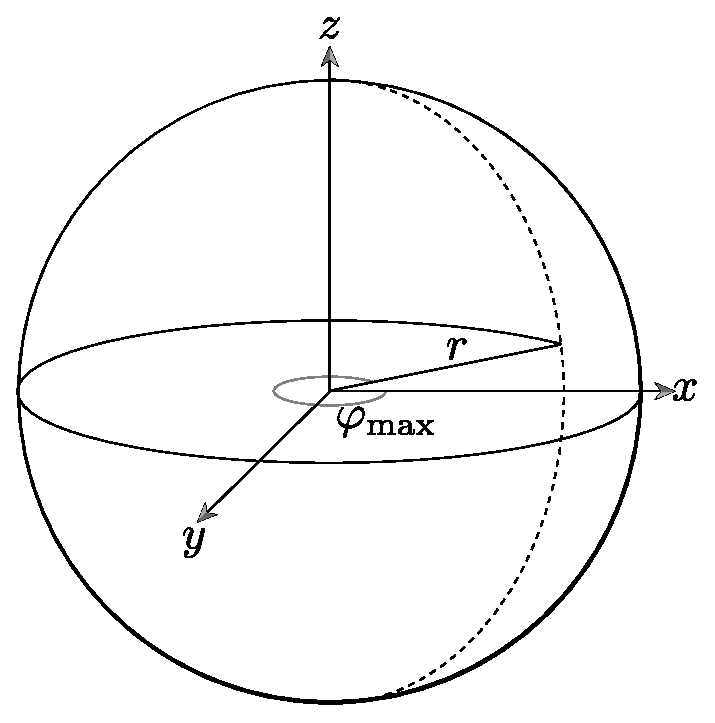
\includegraphics[width=0.35\linewidth]{chap03/Spheresetting.eps}
    \caption{球体形状基本设置。它半径为$r$,球心位于物体空间原点。
        部分球体可以通过指定$\varphi$的最大值描述。}
    \label{fig:3.4}
\end{figure}

我们可以用以下替换将该函数$f(\theta,\varphi)$转换为$[0,1]^2$上的函数$f(u,v)$并
稍微将其一般化以允许部分球体只扫过$\theta\in[\theta_{\min},\theta_{\max}]$和$\varphi\in[0,\varphi_{\max}]$:
\begin{align*}
    \varphi & =u\varphi_{\max}\, ,                              \\
    \theta  & =\theta_{\min}+v(\theta_{\max}-\theta_{\min})\, .
\end{align*}

该形式对纹理贴图特别有用,它能直接用来
将定义在$[0,1]^2$上的纹理映射到球上。
\reffig{3.5}展示了两个球的一张图像;一张网格图像用于展示$(u,v)$参数化。
\begin{figure}[htbp]
    \centering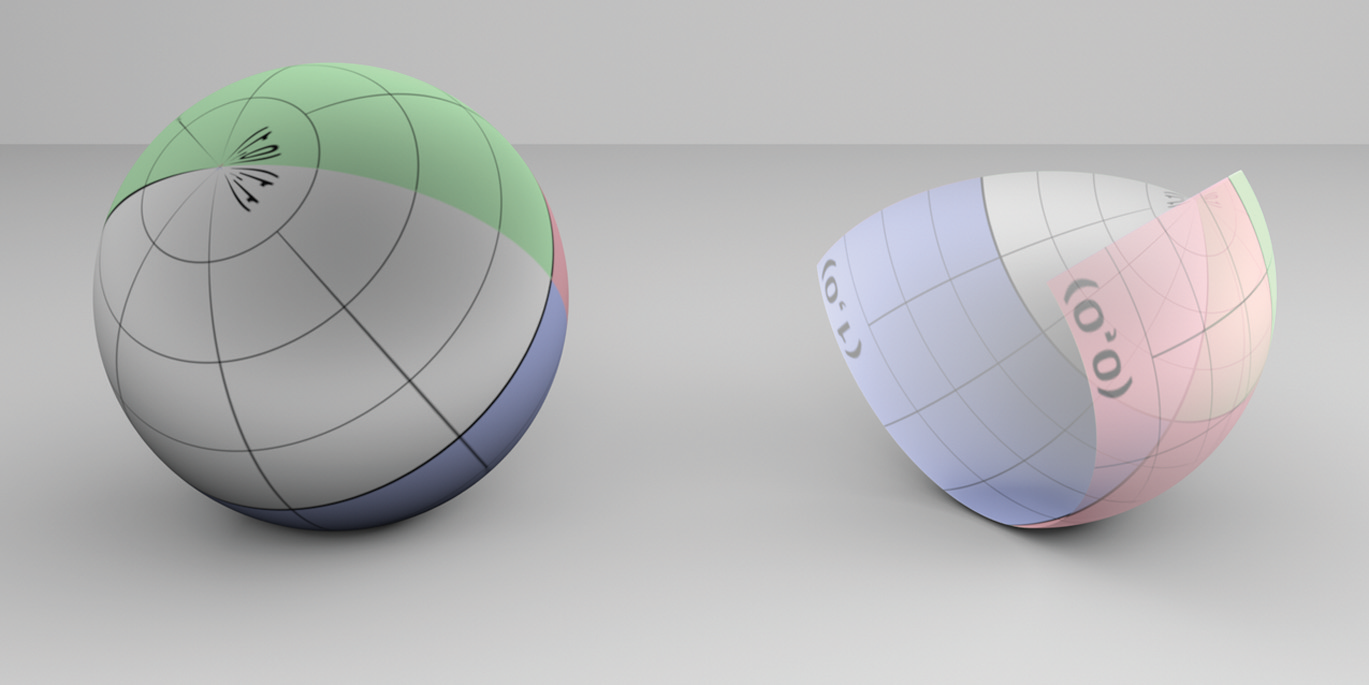
\includegraphics[width=\linewidth]{chap03/twospheres.png}
    \caption{两个球。左边是完整球,右边是部分球($z_{\max}<r$和$\varphi_{\max}<2\pi$)。
        注意纹理贴图用来展示形状$(u,v)$参数化;一极的\protect\keyindex{奇点}{singularity}{}在完整球中可见。}
    \label{fig:3.5}
\end{figure}

当我们描述球形状的实现时,我们将同时利用形状的隐式和参数化描述,
这取决于哪种方式能更自然地解决我们面临的特定问题。

类\refvar{Sphere}{}表示球心在物体空间原点的球体。
其实现在\href{https://github.com/mmp/pbrt-v3/tree/master/src/shapes/sphere.h}{\ttfamily shapes/sphere.h}
和\href{https://github.com/mmp/pbrt-v3/tree/master/src/shapes/sphere.cpp}{\ttfamily shapes/sphere.cpp}文件中。
\begin{lstlisting}
`\initcode{Sphere Declarations}{=}`
class `\initvar{Sphere}{}` : public `\refvar{Shape}{}` {
public:
    `\refcode{Sphere Public Methods}{}`
private:
    `\refcode{Sphere Private Data}{}`
};
\end{lstlisting}

为了在场景中别处放置球体,用户在输入文件里指定球体时必须施加合适的变换。
它同时接收物体到世界和世界到物体的变换作为参数给构造函数,
并将它们传给父类\refvar{Shape}{}的构造函数。

球的半径可以是任意正值,且球的范围可用两种方式截断。
第一,设置最小和最大$z$值;球体分别位于这些平面之下和之上的部分会被切除。
第二,在球面坐标中考虑球的参数化,可设置最大的$\varphi$值。
球体的$\varphi$值扫过从$0$到给定$\varphi_{\max}$的范围,
这样超出$\varphi_{\max}$的$\varphi$值对应的球体部分也被移除。
\begin{lstlisting}
`\initcode{Sphere Public Methods}{=}`
`\refvar{Sphere}{}`(const `\refvar{Transform}{}` *ObjectToWorld, const `\refvar{Transform}{}` *WorldToObject,
       bool reverseOrientation, `\refvar{Float}{}` radius, `\refvar{Float}{}` zMin, `\refvar{Float}{}` zMax,
       `\refvar{Float}{}` phiMax)
    : `\refvar{Shape}{}`(ObjectToWorld, WorldToObject, reverseOrientation),
      `\refvar[Sphere::radius]{radius}{}`(radius), `\refvar[Sphere::zMin]{zMin}{}`(`\refvar{Clamp}{}`(std::min(zMin, zMax), -radius, radius)),
      `\refvar[Sphere::zMax]{zMax}{}`(`\refvar{Clamp}{}`(std::max(zMin, zMax), -radius, radius)),
      `\refvar[Sphere::thetaMin]{thetaMin}{}`(std::acos(`\refvar{Clamp}{}`(zMin / radius, -1, 1))),
      `\refvar[Sphere::thetaMax]{thetaMax}{}`(std::acos(`\refvar{Clamp}{}`(zMax / radius, -1, 1))),
      `\refvar[Sphere::phiMax]{phiMax}{}`(`\refvar{Radians}{}`(`\refvar{Clamp}{}`(phiMax, 0, 360))) { }
\end{lstlisting}
\begin{lstlisting}
`\initcode{Sphere Private Data}{=}`
const `\refvar{Float}{}` `\initvar[Sphere::radius]{radius}{}`;
const `\refvar{Float}{}` `\initvar[Sphere::zMin]{zMin}{}`, `\initvar[Sphere::zMax]{zMax}{}`;
const `\refvar{Float}{}` `\initvar[Sphere::thetaMin]{thetaMin}{}`, `\initvar[Sphere::thetaMax]{thetaMax}{}`, `\initvar[Sphere::phiMax]{phiMax}{}`;
\end{lstlisting}

\subsection{边界}\label{sub:边界2}
计算球体的物体空间边界框很简单。
当要渲染的部分少于整个球体时,这里的实现使用用户提供的$z_{\min}$和$z_{\max}$值来缩紧边界。
然而,当$\varphi_{\max}$少于$\displaystyle\frac{3\pi}{2}$时它并不做额外工作计算更紧的边界框。
该改进留作习题。
\begin{lstlisting}
`\initcode{Sphere Method Definitions}{=}\initnext{SphereMethodDefinitions}`
`\refvar{Bounds3f}{}` `\refvar{Sphere}{}`::`\initvar[Sphere::ObjectBound]{\refvar{ObjectBound}{}}{}`() const {
    return `\refvar{Bounds3f}{}`(`\refvar{Point3f}{}`(-`\refvar[Sphere::radius]{radius}{}`, -`\refvar[Sphere::radius]{radius}{}`, `\refvar[Sphere::zMin]{zMin}{}`),
                    `\refvar{Point3f}{}`( `\refvar[Sphere::radius]{radius}{}`,  `\refvar[Sphere::radius]{radius}{}`, `\refvar[Sphere::zMax]{zMax}{}`));
}
\end{lstlisting}

\subsection{相交测试}\label{sub:相交测试2}
推导光线-球体相交测试的任务被球心位于原点的事实简化了。
然而如果球已被变换到世界空间的另一位置,
则光线与球相交前需要用世界到物体的变换来变到物体空间。
有了物体空间的光线,就能在物体空间执行相交计算了
\footnote{这是计算机图形学的经典主题。
    通过把问题转换为特定受限的情况,就可能更简单高效地做相交测试:
    即因为球总是在$(0,0,0)$,方程的许多项就消掉了。
    这不会失去一般性,因为对于其他位置的球体,适当平移光线即可。}。

下列代码片展示了整个相交方法:
\begin{lstlisting}
`\refcode{Sphere Method Definitions}{+=}\lastnext{SphereMethodDefinitions}`
bool `\refvar{Sphere}{}`::`\initvar[Sphere::Intersect]{\refvar[Shape::Intersect]{Intersect}{}}{}`(const `\refvar{Ray}{}` &r, `\refvar{Float}{}` *tHit,
        `\refvar{SurfaceInteraction}{}` *isect, bool testAlphaTexture) const {
    `\refvar{Float}{}` phi;
    `\refvar{Point3f}{}` pHit;
    `\refcode{Transform Ray to object space}{}`
    `\refcode{Compute quadratic sphere coefficients}{}`
    `\refcode{Solve quadratic equation for t values}{}`
    `\refcode{Compute sphere hit position and $\varphi$}{}`
    `\refcode{Test sphere intersection against clipping parameters}{}`
    `\refcode{Find parametric representation of sphere hit}{}`
    `\refcode{Compute error bounds for sphere intersection}{}`
    `\refcode{Initialize SurfaceInteraction from parametric information}{}`
    `\refcode{Update tHit for quadric intersection}{}`
    return true;
}
\end{lstlisting}

首先,所给世界空间光线被变换到球的物体空间。
相交测试的剩余部分将在那个坐标系内进行。
{\ttfamily oErr}和{\ttfamily dErr}变量分别定界
在变换射线端点和方向时因为施加变换而引入的浮点舍入误差
(更多关于浮点算术和其对于准确光线相交计算实现的更多信息见\refsec{控制舍入误差})。
\begin{lstlisting}
`\initcode{Transform Ray to object space}{=}`
`\refvar{Vector3f}{}` oErr, dErr;
`\refvar{Ray}{}` ray = (*`\refvar{WorldToObject}{}`)(r, &oErr, &dErr);
\end{lstlisting}

如果球心在原点,半径为$r$,则其隐式表示是
\begin{align*}
    x^2+y^2+z^2-r^2=0\, .
\end{align*}

通过将\refeq{2.3}中射线的参数表示代入隐式球方程,我们有
\begin{align*}
    (o_x+td_x)^2+(o_y+td_y)^2+(o_z+td_z)^2=r^2\, .
\end{align*}

注意该方程除了$t$的所有元素都是已知量。
使方程成立的$t$值给出了光线上使隐式球方程成立的参数化位置,
即沿光线与球相交的点。
我们可以展开该方程并整理系数得到$t$的一般二次方程,
\begin{align*}
    at^2+bt+c=0\, ,
\end{align*}
其中\footnote{一些光线追踪器要求规范化射线方向向量,即$a=1$。
    然而如果调用者忘记规范化射线方向则会导致微妙错误。
    当然,该错误可以通过在射线构造函数内规范化方向来避免,
    但这在提供的方向\emph{已经}规范化时会浪费精力。
    为了避免这无用的复杂性,pbrt没有在相交例程中坚持向量规范化。
    这特别有用,因为它减少了将射线变换到物体空间所需的计算量,即不需要规范化。}
\begin{align*}
    a & =d_x^2+d_y^2+d_z^2\, ,       \\
    b & =2(d_xo_x+d_yo_y+d_zo_z)\, , \\
    c & =o_x^2+o_y^2+o_z^2-r^2\, .
\end{align*}

该结果可以直接翻译为源码片。注意在该代码中,
类\refvar{EFloat}{}的而不是\refvar{Float}{}
的实例用于表示浮点值。\refvar{EFloat}{}跟踪累积的浮点舍入误差;
\refsec{控制舍入误差}将讨论它的使用。
至于现在,阅读时可以认为它和\refvar{Float}{}等价。
\begin{lstlisting}
`\initcode{Compute quadratic sphere coefficients}{=}`
`\refcode{Initialize EFloat ray coordinate values}{}`
`\refvar{EFloat}{}` a = dx * dx + dy * dy + dz * dz;
`\refvar{EFloat}{}` b = 2 * (dx * ox + dy * oy + dz * oz);
`\refvar{EFloat}{}` c = ox * ox + oy * oy + oz * oz - `\refvar{EFloat}{}`(`\refvar[Sphere::radius]{radius}{}`) * `\refvar{EFloat}{}`(`\refvar[Sphere::radius]{radius}{}`);
\end{lstlisting}

相交测试用的射线端点和方向值由将射线变换到物体空间的浮点误差界初始化。
\begin{lstlisting}
`\initcode{Initialize EFloat ray coordinate values}{=}`
`\refvar{EFloat}{}` ox(ray.o.x, oErr.x), oy(ray.o.y, oErr.y), oz(ray.o.z, oErr.z);
`\refvar{EFloat}{}` dx(ray.d.x, dErr.x), dy(ray.d.y, dErr.y), dz(ray.d.z, dErr.z);
\end{lstlisting}

二次方程有两个可能的解,给出光线交于球体的零、一或两个非虚数$t$值。
\begin{lstlisting}
`\initcode{Solve quadratic equation for t values}{=}`
`\refvar{EFloat}{}` t0, t1;
if (!`\refvar{Quadratic}{}`(a, b, c, &t0, &t1))
    return false;
`\refcode{Check quadric shape t0 and t1 for nearest intersection}{}`
\end{lstlisting}

实用函数\refvar{Quadratic}{}求解二次方程,
如果没有实数解就返回{\ttfamily false},
如果有则返回{\ttfamily true}并适当设置{\ttfamily t0}和{\ttfamily t1}。
稍后将在\refsub{求解二次方程}\sidenote{译者注:原文此处似乎链接章节错误,已修正。}定义它,
我们会讨论怎样用浮点算术稳定地实现它。

算得的参数化距离{\ttfamily t0}和{\ttfamily t1}跟踪了
原始射线参数的误差和\refvar{Quadratic}{}内累积的误差造成的不确定性;
不确定性区间范围的下界和上界可以使用方法\refvar[LowerBound]{EFloat::LowerBound}{()}和
\refvar[UpperBound]{EFloat::UpperBound}{()}获取。

代码片\refcode{Check quadric shape t0 and t1 for nearest intersection}{}取
两个相交值并确定如果有的话哪一个是最近的有效相交处。
对于有效的相交处,其值必须大于零且小于{\ttfamily ray.\refvar{tMax}{}}。
下列代码使用类\refvar{EFloat}{}提供的误差区间并只接受
明确在范围$(0,$\refvar{tMax}{}$)$内的相交处。

因为$t_0$保证小于或等于$t_1$(且$0$小于\refvar{tMax}{}),
则如果$t_0$大于\refvar{tMax}{}或$t_1$小于$0$,
那么两个相交处都一定超出了考虑范围。
否则,$t_0$是暂时的命中$t$值。
但它可能小于$0$,这时我们忽略它并尝试$t_1$。
如果也超出范围,我们就没有有效相交处。
如果有一个相交处,则初始化{\ttfamily tShapeHit}来保存该相交处的参数$t$值。
\begin{lstlisting}
`\initcode{Check quadric shape t0 and t1 for nearest intersection}{=}`
if (t0.`\refvar{UpperBound}{}`() > ray.`\refvar{tMax}{}` || t1.`\refvar{LowerBound}{}`() <= 0)
    return false;
`\refvar{EFloat}{}` tShapeHit = t0;
if (tShapeHit.`\refvar{LowerBound}{}`() <= 0) {
    tShapeHit = t1;
    if (tShapeHit.`\refvar{UpperBound}{}`() > ray.`\refvar{tMax}{}`)
        return false;
}
\end{lstlisting}
有了射线与完整球体相交的参数距离,
就能按沿射线的偏移量计算交点{\ttfamily pHit}。

接下来需要处理带有截断$z$或$\varphi$范围的部分球体——
必须忽略与截去区域的相交。
实现从计算命中点的$\varphi$值开始。使用球的参数化表示,
\begin{align*}
    \frac{y}{x}=\frac{r\sin\theta\sin\varphi}{r\sin\theta\cos\varphi}=\tan\varphi\, ,
\end{align*}
所以$\displaystyle\varphi=\arctan\frac{y}{x}$。
为了符合球的原始定义,需要将标准库函数{\ttfamily std::atan()}的
结果重新映射为$0$到$2\pi$的值。
\begin{lstlisting}
`\initcode{Compute sphere hit position and $\varphi$}{=}`
pHit = ray((`\refvar{Float}{}`)tShapeHit);
`\refcode{Refine sphere intersection point}{}`
if (pHit.x == 0 && pHit.y == 0) pHit.x = 1e-5f * `\refvar[Sphere::radius]{radius}{}`;
phi = std::atan2(pHit.y, pHit.x);
if (phi < 0) phi += 2 * `\refvar{Pi}{}`;
\end{lstlisting}

由于浮点精度限制,算得的该交点{\ttfamily pHit}可能位于实际球体表面的一侧;
定义于\refsub{定界交点误差}的
代码片\refcode{Refine sphere intersection point}{}会提升该值精度。

现在可以针对$z$和$\varphi$指定的最小值和最大值测试命中点了。
一个细节是如果$z$范围包括了整个球体则跳过$z$测试非常重要;
算得的值{\ttfamily pHit.z}可能因为浮点舍入超出$z$范围一点点,
所以我们应该只在用户希望球体是部分不完整时才执行该测试。
如果$t_0$相交处实际无效,例程就再次尝试$t_1$。
\begin{lstlisting}
`\initcode{Test sphere intersection against clipping parameters}{=}`
if ((`\refvar[Sphere::zMin]{zMin}{}` > -`\refvar[Sphere::radius]{radius}{}` && pHit.z < `\refvar[Sphere::zMin]{zMin}{}`) ||
    (`\refvar[Sphere::zMax]{zMax}{}` <  `\refvar[Sphere::radius]{radius}{}` && pHit.z > `\refvar[Sphere::zMax]{zMax}{}`) || phi > `\refvar[Sphere::phiMax]{phiMax}{}`) {
    if (tShapeHit == t1) return false;
    if (t1.`\refvar{UpperBound}{}`() > ray.`\refvar{tMax}{}`) return false;
    tShapeHit = t1;
    `\refcode{Compute sphere hit position and $\varphi$}{}`
    if ((`\refvar[Sphere::zMin]{zMin}{}` > -`\refvar[Sphere::radius]{radius}{}` && pHit.z < `\refvar[Sphere::zMin]{zMin}{}`) ||
        (`\refvar[Sphere::zMax]{zMax}{}` <  `\refvar[Sphere::radius]{radius}{}` && pHit.z > `\refvar[Sphere::zMax]{zMax}{}`) || phi > `\refvar[Sphere::phiMax]{phiMax}{}`)
        return false;
}
\end{lstlisting}

在例程中的此处,光线一定命中了球体。
接下来方法分别通过缩放之前计算的$\varphi$值来为命中点计算在0到1之间的$u$值,
并基于所给球体的$\theta$值范围通过为命中点计算0到1的$\theta$值来计算$v$值
\sidenote{译者注:这句话太绕了,我投降,请大佬赐教怎么翻译。
    看不懂没关系,去翻翻前面$u,v$与$\varphi,\theta$的关系你就懂了。}。
然后它再求位置的参数化偏导数$\displaystyle\frac{\partial \bm p}{\partial u}$和
$\displaystyle\frac{\partial \bm p}{\partial v}$以及
曲面法线的$\displaystyle\frac{\partial \bm n}{\partial u}$和
$\displaystyle\frac{\partial \bm n}{\partial v}$。
\begin{lstlisting}
`\initcode{Find parametric representation of sphere hit}{=}`
`\refvar{Float}{}` u = phi / `\refvar[Sphere::phiMax]{phiMax}{}`;
`\refvar{Float}{}` theta = std::acos(`\refvar{Clamp}{}`(pHit.z / `\refvar[Sphere::radius]{radius}{}`, -1, 1));
`\refvar{Float}{}` v = (theta - `\refvar[Sphere::thetaMin]{thetaMin}{}`) / (`\refvar[Sphere::thetaMax]{thetaMax}{}` - `\refvar[Sphere::thetaMin]{thetaMin}{}`);
`\refcode{Compute sphere $\partial$p/$\partial$u and $\partial$p/$\partial$v}{}`
`\refcode{Compute sphere $\partial$n/$\partial$u and $\partial$n/$\partial$v}{}`
\end{lstlisting}

计算球上一点的偏导数是个代数小习题。
这里我们将展示怎样计算$\displaystyle\frac{\partial \bm p}{\partial u}$的$x$分量,
$\displaystyle\frac{\partial p_x}{\partial u}$;
其他分量解法相同。使用球的参数化定义,我们有\sidenote{译者注:这里$p_x$与$x$含义相同,以此类推。}
\begin{align*}
    x                               & =r\sin\theta\cos\varphi\, ,                          \\
    \frac{\partial p_x}{\partial u} & =\frac{\partial}{\partial u}(r\sin\theta\cos\varphi) \\
                                    & =r\sin\theta\frac{\partial\cos\varphi}{\partial u}   \\
                                    & =-r\varphi_{\max}\sin\theta\sin\varphi\, .
\end{align*}

基于球$y$坐标的参数化定义进行代换,可以简化为
\begin{align*}
    \frac{\partial p_x}{\partial u}=-\varphi_{\max}y\, .
\end{align*}
同样
\begin{align*}
    \frac{\partial p_y}{\partial u}=\varphi_{\max}x\, ,
\end{align*}
以及
\begin{align*}
    \frac{\partial p_z}{\partial u}=0\, .
\end{align*}

同样过程求得$\displaystyle\frac{\partial \bm p}{\partial v}$,完整结果为
\begin{align*}
    \frac{\partial \bm p}{\partial u} & =(-\varphi_{\max}y,\varphi_{\max}x,0)\, ,                                  \\
    \frac{\partial \bm p}{\partial v} & =(\theta_{\max}-\theta_{\min})(z\cos\varphi,z\sin\varphi,-r\sin\theta)\, .
\end{align*}
\begin{lstlisting}
`\initcode{Compute sphere $\partial$p/$\partial$u and $\partial$p/$\partial$v}{=}`
`\refvar{Float}{}` zRadius = std::sqrt(pHit.x * pHit.x + pHit.y * pHit.y);
`\refvar{Float}{}` invZRadius = 1 / zRadius;
`\refvar{Float}{}` cosPhi = pHit.x * invZRadius;
`\refvar{Float}{}` sinPhi = pHit.y * invZRadius;
`\refvar{Vector3f}{}` dpdu(-`\refvar[Sphere::phiMax]{phiMax}{}` * pHit.y, `\refvar[Sphere::phiMax]{phiMax}{}` * pHit.x, 0);
`\refvar{Vector3f}{}` dpdv = (`\refvar[Sphere::thetaMax]{thetaMax}{}` - `\refvar[Sphere::thetaMin]{thetaMin}{}`) *
    `\refvar{Vector3f}{}`(pHit.z * cosPhi, pHit.z * sinPhi,
             -`\refvar[Sphere::radius]{radius}{}` * std::sin(theta));
\end{lstlisting}

\subsection{法向量的偏导数}\label{sub:法向量的偏导数}
\begin{remark}
    本节含有高级内容,第一次阅读时可以跳过。
\end{remark}

当我们沿表面在$u$和$v$方向移动时,确定法线是怎样变化的也很有用。
例如,第\refchap{纹理}的抗锯齿技术就依赖于该信息来消除物体曲面上反射可见的纹理锯齿。
法线的微分变化量$\displaystyle\frac{\partial \bm n}{\partial u}$和
$\displaystyle\frac{\partial \bm n}{\partial v}$由微分几何学
中\keyindex{曲面的外恩加滕公式}{Weingarten formula of surfaces}{surface曲面}给出
\sidenote{译者注:得名于德国数学家Julius Weingarten。
    相关简要推导详见译者整理补充的\refsec{译者补充:微分几何基础}。
    注意该公式其实隐含了对$\bm n$的规范化要求。
    下面所提的第一基本形式、第二基本形式也是微分几何学中的概念。}:
\begin{align*}
    \frac{\partial \bm n}{\partial u} & =\frac{fF-eG}{EG-F^2}\frac{\partial \bm p}{\partial u}+\frac{eF-fE}{EG-F^2}\frac{\partial \bm p}{\partial v}\, , \\
    \frac{\partial \bm n}{\partial v} & =\frac{gF-fG}{EG-F^2}\frac{\partial \bm p}{\partial u}+\frac{fF-gE}{EG-F^2}\frac{\partial \bm p}{\partial v}\, ,
\end{align*}
其中$E,F$和$G$是\keyindex{第一基本形式}{the first fundamental form}{}的系数,即
\begin{align*}
    E & =\left|\frac{\partial \bm p}{\partial u}\right|^2\, ,                                     \\
    F & =\left(\frac{\partial \bm p}{\partial u}\cdot\frac{\partial \bm p}{\partial v}\right)\, , \\
    G & =\left|\frac{\partial \bm p}{\partial v}\right|^2\, .
\end{align*}

它们可以利用之前算得的$\displaystyle\frac{\partial \bm p}{\partial u}$和$\displaystyle\frac{\partial \bm p}{\partial v}$轻松算出。
$e,f$和$g$是\keyindex{第二基本形式}{the second fundamental form}{}的系数,
\begin{align*}
    e & =\left(\bm n\cdot\frac{\partial^2\bm p}{\partial u^2}\right)\, ,         \\
    f & =\left(\bm n\cdot\frac{\partial^2\bm p}{\partial u\partial v}\right)\, , \\
    g & =\left(\bm n\cdot\frac{\partial^2\bm p}{\partial v^2}\right)\, .
\end{align*}

两个基本形式刻画了曲面的基本度量属性,包括距离、角度和\keyindex{曲率}{curvature}{}的概念;
细节详见微分几何教材例如\citet{gray2017modern}
\sidenote{译者注:此处引用文献改为了新版。}。
为了求$e,f$和$g$,需要计算二阶偏导数$\displaystyle\frac{\partial^2\bm p}{\partial u^2}$等。

对于球体,可以算得二阶导数为:
\begin{align*}
    \frac{\partial^2\bm p}{\partial u^2}         & =-\varphi_{\max}^2(x,y,0)\, ,                                                 \\
    \frac{\partial^2\bm p}{\partial u\partial v} & =(\theta_{\max}-\theta_{\min})z\varphi_{\max}(-\sin\varphi,\cos\varphi,0)\, , \\
    \frac{\partial^2\bm p}{\partial v^2}         & =-(\theta_{\max}-\theta_{\min})^2(x,y,z)\, .
\end{align*}
\begin{lstlisting}
`\initcode{Compute sphere $\partial$n/$\partial$u and $\partial$n/$\partial$v}{=}`
`\refvar{Vector3f}{}` d2Pduu = -`\refvar[Sphere::phiMax]{phiMax}{}` * `\refvar[Sphere::phiMax]{phiMax}{}` * `\refvar{Vector3f}{}`(pHit.x, pHit.y, 0);
`\refvar{Vector3f}{}` d2Pduv = (`\refvar[Sphere::thetaMax]{thetaMax}{}` - `\refvar[Sphere::thetaMin]{thetaMin}{}`) * pHit.z * `\refvar[Sphere::phiMax]{phiMax}{}` *
                  `\refvar{Vector3f}{}`(-sinPhi, cosPhi, 0.);
`\refvar{Vector3f}{}` d2Pdvv = -(`\refvar[Sphere::thetaMax]{thetaMax}{}` - `\refvar[Sphere::thetaMin]{thetaMin}{}`) * (`\refvar[Sphere::thetaMax]{thetaMax}{}` - `\refvar[Sphere::thetaMin]{thetaMin}{}`) *
                  `\refvar{Vector3f}{}`(pHit.x, pHit.y, pHit.z);
`\refcode{Compute coefficients for fundamental forms}{}`
`\refcode{Compute $\partial$n/$\partial$u and $\partial$n/$\partial$v from fundamental form coefficients}{}`
\end{lstlisting}
\begin{lstlisting}
`\initcode{Compute coefficients for fundamental forms}{=}`
`\refvar{Float}{}` E = `\refvar{Dot}{}`(dpdu, dpdu);
`\refvar{Float}{}` F = `\refvar{Dot}{}`(dpdu, dpdv);
`\refvar{Float}{}` G = `\refvar{Dot}{}`(dpdv, dpdv);
`\refvar{Vector3f}{}` N = `\refvar{Normalize}{}`(`\refvar{Cross}{}`(dpdu, dpdv));
`\refvar{Float}{}` e = `\refvar{Dot}{}`(N, d2Pduu);
`\refvar{Float}{}` f = `\refvar{Dot}{}`(N, d2Pduv);
`\refvar{Float}{}` g = `\refvar{Dot}{}`(N, d2Pdvv);
\end{lstlisting}
\begin{lstlisting}
`\initcode{Compute $\partial$n/$\partial$u and $\partial$n/$\partial$v from fundamental form coefficients}{=}`
`\refvar{Float}{}` invEGF2 = 1 / (E * G - F * F);
`\refvar{Normal3f}{}` dndu = `\refvar{Normal3f}{}`((f * F - e * G) * invEGF2 * dpdu + 
                         (e * F - f * E) * invEGF2 * dpdv);
`\refvar{Normal3f}{}` dndv = `\refvar{Normal3f}{}`((g * F - f * G) * invEGF2 * dpdu + 
                         (f * F - g * E) * invEGF2 * dpdv);
\end{lstlisting}

\subsection{SurfaceInteraction 初始化}
计算了曲面参数化和所有相关偏导数后,
可以用该相交处的几何信息初始化结构\refvar{SurfaceInteraction}{}了。
传给\refvar{SurfaceInteraction}{}构造函数的\refvar{pError}{}值
定界了算得的点{\ttfamily pHit}中的舍入误差。
它在稍后于\refsub{定界交点误差}定义的代码片\refcode{Compute error bounds for sphere intersection}{}中初始化。
\begin{lstlisting}
`\initcode{Initialize SurfaceInteraction from parametric information}{=}`
*isect = (*`\refvar{ObjectToWorld}{}`)(
    `\refvar{SurfaceInteraction}{}`(pHit, `\refvar{pError}{}`, `\refvar{Point2f}{}`(u, v), -ray.`\refvar[Ray::d]{d}{}`, dpdu, dpdv,
                       dndu, dndv, ray.`\refvar[Ray::time]{time}{}`, this));
\end{lstlisting}

因为有相交处,已存于{\ttfamily tShapeHit}的光线上的命中参数距离将更新
方法\refvar[Shape::Intersect]{Intersect}{}的参数{\ttfamily tHit}。
如果可能的命中点比已有的相交处更远,则更新{\ttfamily *tHit}能让后续相交测试提前终止。
\begin{lstlisting}
`\initcode{Update tHit for quadric intersection}{=}`
*tHit = (`\refvar{Float}{}`)tShapeHit;
\end{lstlisting}

这里自然会问道:“世界到物体变换对于返回正确的参数距离有何影响呢?”
确实,相交方法已经为物体空间射线求得到相交处的参数距离,
它可能已被平移、旋转、缩放,甚至是从世界空间变换来的。
然而,可以证明在物体空间内到相交处的参数距离正好等于
把射线留在世界空间内并在那里求相交后得到的距离,
因此,{\ttfamily *tHit}可以直接设置。
注意如果物体空间射线的方向在变换后被规范化,那就不是这种情况了,
会需要一个与未规范化射线的长度相关的校正因子。
这是变换后不规范化物体空间射线方向向量的另一个动机。

\refvar{Sphere::IntersectP}{()}例程几乎和\refvar{Sphere::Intersect}{()}一样,
但它不初始化结构\refvar{SurfaceInteraction}{}。
因为方法\refvar[Shape::Intersect]{Intersect}{}和\refvar[Shape::IntersectP]{IntersectP}{()}总是如此接近,
接下来我们不再为剩余形状展示\refvar[Shape::IntersectP]{IntersectP}{()}。
\begin{lstlisting}
`\refcode{Sphere Method Definitions}{+=}\lastnext{SphereMethodDefinitions}`
bool `\refvar{Sphere}{}`::`\initvar[Sphere::IntersectP]{\refvar[Shape::IntersectP]{IntersectP}{}}{}`(const `\refvar{Ray}{}` &r, bool testAlphaTexture) const {
    `\refvar{Float}{}` phi;
    `\refvar{Point3f}{}` pHit;
    `\refcode{Transform Ray to object space}{}`
    `\refcode{Compute quadratic sphere coefficients}{}`
    `\refcode{Solve quadratic equation for t values}{}`
    `\refcode{Compute sphere hit position and $\varphi$}{}`
    `\refcode{Test sphere intersection against clipping parameters}{}`
    return true;
}
\end{lstlisting}

\subsection{表面积}\label{sub:表面积2}
为了计算二次曲面的表面积,我们使用\keyindex{积分学}{integral calculus}{}的标准公式。
如果定义于$x=a$到$x=b$的\keyindex{曲线}{curve}{}$y=f(x)$绕$x$轴旋转,
则所得扫掠曲面的表面积为
\begin{align*}
    2\pi\int_a^b{f(x)\sqrt{1+(f'(x))^2}\mathrm{d}x}\, ,
\end{align*}
其中$f'(x)$表示导数$\displaystyle\frac{\mathrm{d}f}{\mathrm{d}x}$。
因为我们大多数的旋转表面都只是绕轴部分扫掠的,所以我们替代使用公式
\begin{align*}
    \varphi_{\max}\int_a^b{f(x)\sqrt{1+(f'(x))^2}\mathrm{d}x}\, .
\end{align*}

球面是\keyindex{圆弧}{circular arc}{}旋转的曲面。
沿球体$z$轴定义轮廓曲线的函数是
\begin{align*}
    f(z)=\sqrt{r^2-z^2}\, ,
\end{align*}
并且其导数为
\begin{align*}
    f'(z)=-\frac{z}{\sqrt{r^2-z^2}}\, .
\end{align*}

回想球体在$z_{\min}$和$z_{\max}$处被裁剪。因此表面积为
\begin{align*}
    A & =\varphi_{\max}\int_{z_{\min}}^{z_{\max}}{\sqrt{r^2-z^2}\sqrt{1+\frac{z^2}{r^2-z^2}}\mathrm{d}z} \\
      & =\varphi_{\max}\int_{z_{\min}}^{z_{\max}}{\sqrt{r^2-z^2+z^2}\mathrm{d}z}                         \\
      & =\varphi_{\max}\int_{z_{\min}}^{z_{\max}}{r\mathrm{d}z}                                          \\
      & =\varphi_{\max}r(z_{\max}-z_{\min})\, .
\end{align*}

对于完整球体$\varphi_{\max}=2\pi$,$z_{\min}=-r$且$z_{\max}=r$,
所以我们有标准公式$A=4\pi r^2$,确认该公式有意义。
\begin{lstlisting}
`\refcode{Sphere Method Definitions}{+=}\lastnext{SphereMethodDefinitions}`
`\refvar{Float}{}` `\refvar{Sphere}{}`::`\initvar[Sphere::Area]{\refvar[Shape::Area]{Area}{}}{}`() const {
    return `\refvar[Sphere::phiMax]{phiMax}{}` * `\refvar[Sphere::radius]{radius}{}` * (`\refvar[Sphere::zMax]{zMax}{}` - `\refvar[Sphere::zMin]{zMin}{}`);
}
\end{lstlisting}

\section{圆柱体}\label{sec:圆柱体}

另一个有用的二次曲面是\keyindex{圆柱体}{cylinder}{};
pbrt提供以$z$轴为中心的圆柱体\refvar{Shape}{}。
实现在文件\href{https://github.com/mmp/pbrt-v3/tree/master/src/shapes/cylinder.h}{\ttfamily shapes/cylinder.h}和
\href{https://github.com/mmp/pbrt-v3/tree/master/src/shapes/cylinder.cpp}{\ttfamily shapes/cylinder.cpp}内。
用户为圆柱体提供最小和最大$z$值,以及半径和最大扫掠值$\varphi$(\reffig{3.6})。
\begin{figure}[htbp]
    \centering%LaTeX with PSTricks extensions
%%Creator: Inkscape 1.0.1 (3bc2e813f5, 2020-09-07)
%%Please note this file requires PSTricks extensions
\psset{xunit=.35pt,yunit=.35pt,runit=.35pt}
\begin{pspicture}(448.67001343,346.17999268)
{
\newrgbcolor{curcolor}{0.50196081 0.50196081 0.50196081}
\pscustom[linewidth=1,linecolor=curcolor]
{
\newpath
\moveto(247.69,277.90999268)
\curveto(247.69,272.81999268)(231.64,268.68999268)(211.84,268.68999268)
\curveto(192.04,268.68999268)(176,272.81999268)(176,277.90999268)
\curveto(176,282.99999268)(192.05,287.12999268)(211.84,287.12999268)
\curveto(222.98,287.12999268)(232.93,285.82999268)(239.5,283.77999268)
}
}
{
\newrgbcolor{curcolor}{0 0 0}
\pscustom[linewidth=1,linecolor=curcolor]
{
\newpath
\moveto(211.83000183,101.72999573)
\lineto(211.83000183,314.95999336)
}
}
{
\newrgbcolor{curcolor}{0 0 0}
\pscustom[linestyle=none,fillstyle=solid,fillcolor=curcolor]
{
\newpath
\moveto(217.34,310.04999268)
\lineto(211.83,314.30999268)
\lineto(206.33,310.04999268)
\lineto(211.83,323.05999268)
\closepath
}
}
{
\newrgbcolor{curcolor}{0.65098041 0.65098041 0.65098041}
\pscustom[linestyle=none,fillstyle=solid,fillcolor=curcolor]
{
\newpath
\moveto(216.13,311.60999268)
\lineto(211.83,321.74999268)
\lineto(211.83,314.93999268)
\closepath
}
}
{
\newrgbcolor{curcolor}{0.40000001 0.40000001 0.40000001}
\pscustom[linestyle=none,fillstyle=solid,fillcolor=curcolor]
{
\newpath
\moveto(207.53,311.60999268)
\lineto(211.83,321.74999268)
\lineto(211.83,314.93999268)
\closepath
}
}
{
\newrgbcolor{curcolor}{0 0 0}
\pscustom[linewidth=1,linecolor=curcolor]
{
\newpath
\moveto(211.83000183,102.07998657)
\lineto(132.74000549,23.97998047)
}
}
{
\newrgbcolor{curcolor}{0 0 0}
\pscustom[linestyle=none,fillstyle=solid,fillcolor=curcolor]
{
\newpath
\moveto(132.37,31.34999268)
\lineto(133.2,24.43999268)
\lineto(140.1,23.50999268)
\lineto(126.97,18.28999268)
\closepath
}
}
{
\newrgbcolor{curcolor}{0.65098041 0.65098041 0.65098041}
\pscustom[linestyle=none,fillstyle=solid,fillcolor=curcolor]
{
\newpath
\moveto(132.1,29.38999268)
\lineto(127.91,19.20999268)
\lineto(132.75,23.98999268)
\closepath
}
}
{
\newrgbcolor{curcolor}{0.40000001 0.40000001 0.40000001}
\pscustom[linestyle=none,fillstyle=solid,fillcolor=curcolor]
{
\newpath
\moveto(138.14,23.27999268)
\lineto(127.91,19.20999268)
\lineto(132.75,23.98999268)
\closepath
}
}
{
\newrgbcolor{curcolor}{0 0 0}
\pscustom[linewidth=1,linecolor=curcolor]
{
\newpath
\moveto(211.57000732,102.31999207)
\lineto(424.79998779,102.31999207)
}
}
{
\newrgbcolor{curcolor}{0 0 0}
\pscustom[linestyle=none,fillstyle=solid,fillcolor=curcolor]
{
\newpath
\moveto(419.89,96.80999268)
\lineto(424.15,102.31999268)
\lineto(419.89,107.81999268)
\lineto(432.91,102.31999268)
\closepath
}
}
{
\newrgbcolor{curcolor}{0.65098041 0.65098041 0.65098041}
\pscustom[linestyle=none,fillstyle=solid,fillcolor=curcolor]
{
\newpath
\moveto(421.45,98.01999268)
\lineto(431.59,102.31999268)
\lineto(424.78,102.31999268)
\closepath
}
}
{
\newrgbcolor{curcolor}{0.40000001 0.40000001 0.40000001}
\pscustom[linestyle=none,fillstyle=solid,fillcolor=curcolor]
{
\newpath
\moveto(421.45,106.61999268)
\lineto(431.59,102.31999268)
\lineto(424.78,102.31999268)
\closepath
}
}
{
\newrgbcolor{curcolor}{0 0 0}
\pscustom[linewidth=1,linecolor=curcolor]
{
\newpath
\moveto(350.83000183,277.73999023)
\curveto(350.83000183,286.35502645)(316.96111637,294.12183088)(265.01762877,297.41847591)
\curveto(213.07424711,300.71511422)(153.28645653,298.89232333)(113.53009079,292.80059904)
\curveto(73.77372505,286.70887475)(61.87766115,277.5478076)(83.39248224,269.58871089)
\curveto(104.90734722,261.62959795)(155.59577355,256.439991)(211.82000732,256.439991)
\curveto(268.0442411,256.439991)(318.73266743,261.62959795)(340.2475324,269.58871089)
\curveto(361.7623535,277.5478076)(349.86628959,286.70887475)(310.10992386,292.80059904)
\curveto(270.35355812,298.89232333)(210.56576754,300.71511422)(158.62238587,297.41847591)
\curveto(106.67889828,294.12183088)(72.81001282,286.35502645)(72.81001282,277.73999023)
\curveto(72.81001282,269.12495402)(106.67889828,261.35814959)(158.62238587,258.06150455)
\curveto(210.56576754,254.76486625)(270.35355812,256.58765714)(310.10992386,262.67938143)
\curveto(349.86628959,268.77110572)(361.7623535,277.93217287)(340.2475324,285.89126957)
\curveto(318.73266743,293.85038252)(268.0442411,299.03998947)(211.82000732,299.03998947)
\curveto(155.59577355,299.03998947)(104.90734722,293.85038252)(83.39248224,285.89126957)
\curveto(61.87766115,277.93217287)(73.77372505,268.77110572)(113.53009079,262.67938143)
\curveto(153.28645653,256.58765714)(213.07424711,254.76486625)(265.01762877,258.06150455)
\curveto(316.96111637,261.35814959)(350.83000183,269.12495402)(350.83000183,277.73999023)
\closepath
}
}
{
\newrgbcolor{curcolor}{0 0 0}
\pscustom[linewidth=1,linecolor=curcolor]
{
\newpath
\moveto(211.74000549,278.00999451)
\lineto(291.57000732,295.15999222)
}
}
{
\newrgbcolor{curcolor}{0 0 0}
\pscustom[linewidth=1,linecolor=curcolor]
{
\newpath
\moveto(211.88999939,278.00999451)
\lineto(350.79000854,278.00999451)
}
}
{
\newrgbcolor{curcolor}{0 0 0}
\pscustom[linewidth=1,linecolor=curcolor]
{
\newpath
\moveto(350.72999573,140.75)
\curveto(350.72999573,149.36503621)(316.86111027,157.13184065)(264.91762267,160.42848568)
\curveto(212.97424101,163.72512399)(153.18645043,161.90233309)(113.43008469,155.8106088)
\curveto(73.67371895,149.71888452)(61.77765504,140.55781737)(83.29247614,132.59872066)
\curveto(104.80734112,124.63960772)(155.49576745,119.45000076)(211.72000122,119.45000076)
\curveto(267.94423499,119.45000076)(318.63266133,124.63960772)(340.1475263,132.59872066)
\curveto(361.6623474,140.55781737)(349.76628349,149.71888452)(310.00991775,155.8106088)
\curveto(270.25355201,161.90233309)(210.46576143,163.72512399)(158.52237977,160.42848568)
\curveto(106.57889217,157.13184065)(72.71000671,149.36503621)(72.71000671,140.75)
\curveto(72.71000671,132.13496379)(106.57889217,124.36815935)(158.52237977,121.07151432)
\curveto(210.46576143,117.77487601)(270.25355201,119.59766691)(310.00991775,125.6893912)
\curveto(349.76628349,131.78111548)(361.6623474,140.94218263)(340.1475263,148.90127934)
\curveto(318.63266133,156.86039228)(267.94423499,162.04999924)(211.72000122,162.04999924)
\curveto(155.49576745,162.04999924)(104.80734112,156.86039228)(83.29247614,148.90127934)
\curveto(61.77765504,140.94218263)(73.67371895,131.78111548)(113.43008469,125.6893912)
\curveto(153.18645043,119.59766691)(212.97424101,117.77487601)(264.91762267,121.07151432)
\curveto(316.86111027,124.36815935)(350.72999573,132.13496379)(350.72999573,140.75)
\closepath
}
}
{
\newrgbcolor{curcolor}{0 0 0}
\pscustom[linewidth=1,linecolor=curcolor]
{
\newpath
\moveto(72.76999664,277.96999359)
\lineto(72.76999664,140.83999634)
}
}
{
\newrgbcolor{curcolor}{0 0 0}
\pscustom[linewidth=1,linecolor=curcolor]
{
\newpath
\moveto(350.79998779,278.11999512)
\lineto(350.79998779,140.22999573)
}
}
{
\newrgbcolor{curcolor}{0 0 0}
\pscustom[linewidth=1,linecolor=curcolor]
{
\newpath
\moveto(68.01000214,140.95999146)
\lineto(33.52000046,140.95999146)
}
}
{
\newrgbcolor{curcolor}{0 0 0}
\pscustom[linewidth=1,linecolor=curcolor]
{
\newpath
\moveto(68.01000214,277.78999329)
\lineto(33.52000046,277.78999329)
}
}
{
\newrgbcolor{curcolor}{0 0 0}
\pscustom[linestyle=none,fillstyle=solid,fillcolor=curcolor]
{
\newpath
\moveto(282.46993563,265.46999408)
\curveto(282.39181063,265.07936908)(282.23556063,264.49343158)(282.23556063,264.37624408)
\curveto(282.23556063,263.94655658)(282.58712313,263.71218158)(282.97774813,263.71218158)
\curveto(283.29024813,263.71218158)(283.71993563,263.90749408)(283.91524813,264.41530658)
\curveto(283.95431063,264.49343158)(284.77462313,267.89186908)(284.89181063,268.36061908)
\curveto(285.08712313,269.18093158)(285.55587313,270.89968158)(285.67306063,271.60280658)
\curveto(285.79024813,271.91530658)(286.49337313,273.08718158)(287.07931063,273.63405658)
\curveto(287.27462313,273.79030658)(288.01681063,274.45436908)(289.07149813,274.45436908)
\curveto(289.73556063,274.45436908)(290.08712313,274.14186908)(290.12618563,274.14186908)
\curveto(289.38399813,274.02468158)(288.83712313,273.43874408)(288.83712313,272.77468158)
\curveto(288.83712313,272.38405658)(289.11056063,271.91530658)(289.77462313,271.91530658)
\curveto(290.43868563,271.91530658)(291.14181063,272.50124408)(291.14181063,273.39968158)
\curveto(291.14181063,274.25905658)(290.36056063,275.00124408)(289.07149813,275.00124408)
\curveto(287.46993563,275.00124408)(286.37618563,273.79030658)(285.90743563,273.08718158)
\curveto(285.67306063,274.21999408)(284.77462313,275.00124408)(283.60274813,275.00124408)
\curveto(282.46993563,275.00124408)(282.00118563,274.02468158)(281.76681063,273.59499408)
\curveto(281.33712313,272.73561908)(281.02462313,271.25124408)(281.02462313,271.17311908)
\curveto(281.02462313,270.89968158)(281.25899813,270.89968158)(281.29806063,270.89968158)
\curveto(281.57149813,270.89968158)(281.57149813,270.93874408)(281.72774813,271.48561908)
\curveto(282.15743563,273.24343158)(282.66524813,274.45436908)(283.56368563,274.45436908)
\curveto(283.95431063,274.45436908)(284.30587313,274.25905658)(284.30587313,273.32155658)
\curveto(284.30587313,272.77468158)(284.22774813,272.50124408)(283.91524813,271.21218158)
\closepath
\moveto(282.46993563,265.46999408)
}
}
{
\newrgbcolor{curcolor}{0 0 0}
\pscustom[linestyle=none,fillstyle=solid,fillcolor=curcolor]
{
\newpath
\moveto(442.23157013,104.08531158)
\curveto(442.38782013,104.71031158)(442.97375763,107.01499908)(444.69250763,107.01499908)
\curveto(444.80969513,107.01499908)(445.43469513,107.01499908)(445.94250763,106.70249908)
\curveto(445.23938263,106.54624908)(444.77063263,105.96031158)(444.77063263,105.33531158)
\curveto(444.77063263,104.94468658)(445.04407013,104.47593658)(445.70813263,104.47593658)
\curveto(446.25500763,104.47593658)(447.03625763,104.90562408)(447.03625763,105.92124908)
\curveto(447.03625763,107.21031158)(445.59094513,107.56187408)(444.73157013,107.56187408)
\curveto(443.28625763,107.56187408)(442.42688263,106.23374908)(442.11438263,105.68687408)
\curveto(441.48938263,107.32749908)(440.16125763,107.56187408)(439.41907013,107.56187408)
\curveto(436.84094513,107.56187408)(435.39563263,104.35874908)(435.39563263,103.73374908)
\curveto(435.39563263,103.46031158)(435.66907013,103.46031158)(435.70813263,103.46031158)
\curveto(435.90344513,103.46031158)(435.98157013,103.53843658)(436.02063263,103.73374908)
\curveto(436.88000763,106.38999908)(438.52063263,107.01499908)(439.38000763,107.01499908)
\curveto(439.84875763,107.01499908)(440.70813263,106.78062408)(440.70813263,105.33531158)
\curveto(440.70813263,104.55406158)(440.27844513,102.91343658)(439.38000763,99.39781158)
\curveto(438.98938263,97.87437408)(438.09094513,96.81968658)(436.99719513,96.81968658)
\curveto(436.84094513,96.81968658)(436.29407013,96.81968658)(435.74719513,97.13218658)
\curveto(436.37219513,97.28843658)(436.91907013,97.79624908)(436.91907013,98.49937408)
\curveto(436.91907013,99.16343658)(436.37219513,99.35874908)(436.02063263,99.35874908)
\curveto(435.23938263,99.35874908)(434.65344513,98.73374908)(434.65344513,97.91343658)
\curveto(434.65344513,96.78062408)(435.86438263,96.27281158)(436.95813263,96.27281158)
\curveto(438.63782013,96.27281158)(439.53625763,98.03062408)(439.57532013,98.14781158)
\curveto(439.88782013,97.24937408)(440.78625763,96.27281158)(442.27063263,96.27281158)
\curveto(444.84875763,96.27281158)(446.25500763,99.47593658)(446.25500763,100.10093658)
\curveto(446.25500763,100.37437408)(446.05969513,100.37437408)(445.98157013,100.37437408)
\curveto(445.74719513,100.37437408)(445.70813263,100.25718658)(445.63000763,100.10093658)
\curveto(444.80969513,97.40562408)(443.13000763,96.81968658)(442.34875763,96.81968658)
\curveto(441.37219513,96.81968658)(440.98157013,97.60093658)(440.98157013,98.46031158)
\curveto(440.98157013,99.00718658)(441.09875763,99.55406158)(441.37219513,100.64781158)
\closepath
\moveto(442.23157013,104.08531158)
}
}
{
\newrgbcolor{curcolor}{0 0 0}
\pscustom[linestyle=none,fillstyle=solid,fillcolor=curcolor]
{
\newpath
\moveto(124.36640263,18.72960658)
\curveto(124.48359013,19.08116908)(124.48359013,19.12023158)(124.48359013,19.31554408)
\curveto(124.48359013,19.74523158)(124.13202763,19.97960658)(123.74140263,19.97960658)
\curveto(123.50702763,19.97960658)(123.11640263,19.82335658)(122.88202763,19.47179408)
\curveto(122.84296513,19.31554408)(122.60859013,18.57335658)(122.53046513,18.10460658)
\curveto(122.33515263,17.47960658)(122.17890263,16.77648158)(122.02265263,16.11241908)
\lineto(120.88984013,11.62023158)
\curveto(120.81171513,11.26866908)(119.71796513,9.51085658)(118.07734013,9.51085658)
\curveto(116.82734013,9.51085658)(116.55390263,10.60460658)(116.55390263,11.54210658)
\curveto(116.55390263,12.67491908)(116.98359013,14.23741908)(117.80390263,16.42491908)
\curveto(118.19452763,17.44054408)(118.31171513,17.71398158)(118.31171513,18.22179408)
\curveto(118.31171513,19.31554408)(117.53046513,20.25304408)(116.28046513,20.25304408)
\curveto(113.89765263,20.25304408)(112.99921513,16.62023158)(112.99921513,16.42491908)
\curveto(112.99921513,16.15148158)(113.23359013,16.15148158)(113.27265263,16.15148158)
\curveto(113.54609013,16.15148158)(113.54609013,16.22960658)(113.66327763,16.62023158)
\curveto(114.36640263,18.96398158)(115.34296513,19.70616908)(116.20234013,19.70616908)
\curveto(116.39765263,19.70616908)(116.82734013,19.70616908)(116.82734013,18.92491908)
\curveto(116.82734013,18.29991908)(116.55390263,17.63585658)(116.39765263,17.16710658)
\curveto(115.38202763,14.51085658)(114.95234013,13.10460658)(114.95234013,11.93273158)
\curveto(114.95234013,9.70616908)(116.51484013,8.96398158)(117.99921513,8.96398158)
\curveto(118.97577763,8.96398158)(119.79609013,9.39366908)(120.49921513,10.09679408)
\curveto(120.18671513,8.80773158)(119.87421513,7.55773158)(118.89765263,6.22960658)
\curveto(118.23359013,5.40929408)(117.29609013,4.66710658)(116.16327763,4.66710658)
\curveto(115.81171513,4.66710658)(114.67890263,4.74523158)(114.24921513,5.72179408)
\curveto(114.63984013,5.72179408)(114.99140263,5.72179408)(115.30390263,6.03429408)
\curveto(115.57734013,6.22960658)(115.81171513,6.58116908)(115.81171513,7.04991908)
\curveto(115.81171513,7.83116908)(115.14765263,7.90929408)(114.91327763,7.90929408)
\curveto(114.32734013,7.90929408)(113.50702763,7.51866908)(113.50702763,6.30773158)
\curveto(113.50702763,5.05773158)(114.60077763,4.12023158)(116.16327763,4.12023158)
\curveto(118.70234013,4.12023158)(121.28046513,6.38585658)(121.98359013,9.19835658)
\closepath
\moveto(124.36640263,18.72960658)
}
}
{
\newrgbcolor{curcolor}{0 0 0}
\pscustom[linestyle=none,fillstyle=solid,fillcolor=curcolor]
{
\newpath
\moveto(208.32254713,328.08682158)
\curveto(209.65067213,329.53213408)(210.39285963,330.15713408)(211.29129713,330.93838408)
\curveto(211.29129713,330.93838408)(212.81473463,332.26650908)(213.71317213,333.16494658)
\curveto(216.09598463,335.46963408)(216.64285963,336.68057158)(216.64285963,336.79775908)
\curveto(216.64285963,337.03213408)(216.40848463,337.03213408)(216.36942213,337.03213408)
\curveto(216.17410963,337.03213408)(216.13504713,336.99307158)(215.97879713,336.75869658)
\curveto(215.23660963,335.54775908)(214.72879713,335.15713408)(214.14285963,335.15713408)
\curveto(213.51785963,335.15713408)(213.24442213,335.54775908)(212.85379713,335.97744658)
\curveto(212.38504713,336.52432158)(211.95535963,337.03213408)(211.13504713,337.03213408)
\curveto(209.26004713,337.03213408)(208.12723463,334.72744658)(208.12723463,334.18057158)
\curveto(208.12723463,334.06338408)(208.20535963,333.90713408)(208.40067213,333.90713408)
\curveto(208.63504713,333.90713408)(208.67410963,334.02432158)(208.75223463,334.18057158)
\curveto(209.22098463,335.35244658)(210.66629713,335.35244658)(210.86160963,335.35244658)
\curveto(211.36942213,335.35244658)(211.83817213,335.19619658)(212.42410963,335.00088408)
\curveto(213.43973463,334.61025908)(213.71317213,334.61025908)(214.33817213,334.61025908)
\curveto(213.43973463,333.55557158)(211.36942213,331.75869658)(210.90067213,331.36807158)
\lineto(208.63504713,329.25869658)
\curveto(206.95535963,327.57900908)(206.05692213,326.17275908)(206.05692213,325.97744658)
\curveto(206.05692213,325.74307158)(206.33035963,325.74307158)(206.36942213,325.74307158)
\curveto(206.56473463,325.74307158)(206.60379713,325.78213408)(206.76004713,326.05557158)
\curveto(207.34598463,326.95400908)(208.08817213,327.61807158)(208.90848463,327.61807158)
\curveto(209.45535963,327.61807158)(209.72879713,327.38369658)(210.35379713,326.68057158)
\curveto(210.74442213,326.13369658)(211.21317213,325.74307158)(211.91629713,325.74307158)
\curveto(214.41629713,325.74307158)(215.86160963,328.90713408)(215.86160963,329.57119658)
\curveto(215.86160963,329.68838408)(215.74442213,329.84463408)(215.54910963,329.84463408)
\curveto(215.31473463,329.84463408)(215.27567213,329.68838408)(215.19754713,329.49307158)
\curveto(214.61160963,327.89150908)(213.01004713,327.42275908)(212.18973463,327.42275908)
\curveto(211.72098463,327.42275908)(211.25223463,327.57900908)(210.74442213,327.73525908)
\curveto(209.88504713,328.04775908)(209.49442213,328.16494658)(208.98660963,328.16494658)
\curveto(208.94754713,328.16494658)(208.55692213,328.16494658)(208.32254713,328.08682158)
\closepath
\moveto(208.32254713,328.08682158)
}
}
{
\newrgbcolor{curcolor}{0 0 0}
\pscustom[linestyle=none,fillstyle=solid,fillcolor=curcolor]
{
\newpath
\moveto(3.87147013,135.85697268)
\curveto(5.19959513,137.30228518)(5.94178263,137.92728518)(6.84022013,138.70853518)
\curveto(6.84022013,138.70853518)(8.36365763,140.03666018)(9.26209513,140.93509768)
\curveto(11.64490763,143.23978518)(12.19178263,144.45072268)(12.19178263,144.56791018)
\curveto(12.19178263,144.80228518)(11.95740763,144.80228518)(11.91834513,144.80228518)
\curveto(11.72303263,144.80228518)(11.68397013,144.76322268)(11.52772013,144.52884768)
\curveto(10.78553263,143.31791018)(10.27772013,142.92728518)(9.69178263,142.92728518)
\curveto(9.06678263,142.92728518)(8.79334513,143.31791018)(8.40272013,143.74759768)
\curveto(7.93397013,144.29447268)(7.50428263,144.80228518)(6.68397013,144.80228518)
\curveto(4.80897013,144.80228518)(3.67615763,142.49759768)(3.67615763,141.95072268)
\curveto(3.67615763,141.83353518)(3.75428263,141.67728518)(3.94959513,141.67728518)
\curveto(4.18397013,141.67728518)(4.22303263,141.79447268)(4.30115763,141.95072268)
\curveto(4.76990763,143.12259768)(6.21522013,143.12259768)(6.41053263,143.12259768)
\curveto(6.91834513,143.12259768)(7.38709513,142.96634768)(7.97303263,142.77103518)
\curveto(8.98865763,142.38041018)(9.26209513,142.38041018)(9.88709513,142.38041018)
\curveto(8.98865763,141.32572268)(6.91834513,139.52884768)(6.44959513,139.13822268)
\lineto(4.18397013,137.02884768)
\curveto(2.50428263,135.34916018)(1.60584513,133.94291018)(1.60584513,133.74759768)
\curveto(1.60584513,133.51322268)(1.87928263,133.51322268)(1.91834513,133.51322268)
\curveto(2.11365763,133.51322268)(2.15272013,133.55228518)(2.30897013,133.82572268)
\curveto(2.89490763,134.72416018)(3.63709513,135.38822268)(4.45740763,135.38822268)
\curveto(5.00428263,135.38822268)(5.27772013,135.15384768)(5.90272013,134.45072268)
\curveto(6.29334513,133.90384768)(6.76209513,133.51322268)(7.46522013,133.51322268)
\curveto(9.96522013,133.51322268)(11.41053263,136.67728518)(11.41053263,137.34134768)
\curveto(11.41053263,137.45853518)(11.29334513,137.61478518)(11.09803263,137.61478518)
\curveto(10.86365763,137.61478518)(10.82459513,137.45853518)(10.74647013,137.26322268)
\curveto(10.16053263,135.66166018)(8.55897013,135.19291018)(7.73865763,135.19291018)
\curveto(7.26990763,135.19291018)(6.80115763,135.34916018)(6.29334513,135.50541018)
\curveto(5.43397013,135.81791018)(5.04334513,135.93509768)(4.53553263,135.93509768)
\curveto(4.49647013,135.93509768)(4.10584513,135.93509768)(3.87147013,135.85697268)
\closepath
\moveto(3.87147013,135.85697268)
}
}
{
\newrgbcolor{curcolor}{0 0 0}
\pscustom[linestyle=none,fillstyle=solid,fillcolor=curcolor]
{
\newpath
\moveto(26.46958414,135.32508944)
\curveto(26.46958414,136.84852694)(25.68833414,137.74696444)(23.85239664,137.74696444)
\curveto(22.44614664,137.74696444)(21.50864664,137.00477694)(21.03989664,136.10633944)
\curveto(20.68833414,137.35633944)(19.75083414,137.74696444)(18.50083414,137.74696444)
\curveto(17.05552164,137.74696444)(16.15708414,136.96571444)(15.64927164,136.02821444)
\lineto(15.64927164,137.74696444)
\lineto(13.07114664,137.55165194)
\lineto(13.07114664,136.92665194)
\curveto(14.24302164,136.92665194)(14.39927164,136.80946444)(14.39927164,135.95008944)
\lineto(14.39927164,131.41883944)
\curveto(14.39927164,130.67665194)(14.20395914,130.67665194)(13.07114664,130.67665194)
\lineto(13.07114664,130.05165194)
\curveto(13.11020914,130.05165194)(14.32114664,130.12977694)(15.06333414,130.12977694)
\curveto(15.68833414,130.12977694)(16.89927164,130.05165194)(17.05552164,130.05165194)
\lineto(17.05552164,130.67665194)
\curveto(15.92270914,130.67665194)(15.76645914,130.67665194)(15.76645914,131.41883944)
\lineto(15.76645914,134.58290194)
\curveto(15.76645914,136.37977694)(17.21177164,137.23915194)(18.34458414,137.23915194)
\curveto(19.55552164,137.23915194)(19.71177164,136.30165194)(19.71177164,135.40321444)
\lineto(19.71177164,131.41883944)
\curveto(19.71177164,130.67665194)(19.55552164,130.67665194)(18.42270914,130.67665194)
\lineto(18.42270914,130.05165194)
\curveto(18.46177164,130.05165194)(19.67270914,130.12977694)(20.41489664,130.12977694)
\curveto(21.03989664,130.12977694)(22.25083414,130.05165194)(22.40708414,130.05165194)
\lineto(22.40708414,130.67665194)
\curveto(21.27427164,130.67665194)(21.11802164,130.67665194)(21.11802164,131.41883944)
\lineto(21.11802164,134.58290194)
\curveto(21.11802164,136.37977694)(22.56333414,137.23915194)(23.69614664,137.23915194)
\curveto(24.90708414,137.23915194)(25.06333414,136.30165194)(25.06333414,135.40321444)
\lineto(25.06333414,131.41883944)
\curveto(25.06333414,130.67665194)(24.90708414,130.67665194)(23.77427164,130.67665194)
\lineto(23.77427164,130.05165194)
\curveto(23.81333414,130.05165194)(25.02427164,130.12977694)(25.76645914,130.12977694)
\curveto(26.39145914,130.12977694)(27.60239664,130.05165194)(27.75864664,130.05165194)
\lineto(27.75864664,130.67665194)
\curveto(26.62583414,130.67665194)(26.46958414,130.67665194)(26.46958414,131.41883944)
\closepath
\moveto(26.46958414,135.32508944)
}
}
{
\newrgbcolor{curcolor}{0 0 0}
\pscustom[linestyle=none,fillstyle=solid,fillcolor=curcolor]
{
\newpath
\moveto(32.16780726,140.79383944)
\curveto(32.16780726,141.30165194)(31.73811976,141.80946444)(31.15218226,141.80946444)
\curveto(30.64436976,141.80946444)(30.17561976,141.37977694)(30.17561976,140.79383944)
\curveto(30.17561976,140.16883944)(30.68343226,139.77821444)(31.15218226,139.77821444)
\curveto(31.73811976,139.77821444)(32.16780726,140.20790194)(32.16780726,140.79383944)
\closepath
\moveto(29.51155726,137.55165194)
\lineto(29.51155726,136.92665194)
\curveto(30.60530726,136.92665194)(30.76155726,136.80946444)(30.76155726,135.95008944)
\lineto(30.76155726,131.41883944)
\curveto(30.76155726,130.67665194)(30.60530726,130.67665194)(29.47249476,130.67665194)
\lineto(29.47249476,130.05165194)
\curveto(29.51155726,130.05165194)(30.72249476,130.12977694)(31.42561976,130.12977694)
\curveto(32.05061976,130.12977694)(32.67561976,130.09071444)(33.26155726,130.05165194)
\lineto(33.26155726,130.67665194)
\curveto(32.24593226,130.67665194)(32.08968226,130.67665194)(32.08968226,131.41883944)
\lineto(32.08968226,137.74696444)
\closepath
\moveto(29.51155726,137.55165194)
}
}
{
\newrgbcolor{curcolor}{0 0 0}
\pscustom[linestyle=none,fillstyle=solid,fillcolor=curcolor]
{
\newpath
\moveto(43.11862055,135.32508944)
\curveto(43.11862055,136.84852694)(42.37643305,137.74696444)(40.50143305,137.74696444)
\curveto(39.05612055,137.74696444)(38.15768305,136.96571444)(37.64987055,136.02821444)
\lineto(37.64987055,137.74696444)
\lineto(35.07174555,137.55165194)
\lineto(35.07174555,136.92665194)
\curveto(36.24362055,136.92665194)(36.39987055,136.80946444)(36.39987055,135.95008944)
\lineto(36.39987055,131.41883944)
\curveto(36.39987055,130.67665194)(36.20455805,130.67665194)(35.07174555,130.67665194)
\lineto(35.07174555,130.05165194)
\curveto(35.11080805,130.05165194)(36.32174555,130.12977694)(37.06393305,130.12977694)
\curveto(37.68893305,130.12977694)(38.89987055,130.05165194)(39.05612055,130.05165194)
\lineto(39.05612055,130.67665194)
\curveto(37.92330805,130.67665194)(37.76705805,130.67665194)(37.76705805,131.41883944)
\lineto(37.76705805,134.58290194)
\curveto(37.76705805,136.37977694)(39.21237055,137.23915194)(40.34518305,137.23915194)
\curveto(41.55612055,137.23915194)(41.71237055,136.30165194)(41.71237055,135.40321444)
\lineto(41.71237055,131.41883944)
\curveto(41.71237055,130.67665194)(41.55612055,130.67665194)(40.42330805,130.67665194)
\lineto(40.42330805,130.05165194)
\curveto(40.46237055,130.05165194)(41.67330805,130.12977694)(42.41549555,130.12977694)
\curveto(43.04049555,130.12977694)(44.25143305,130.05165194)(44.40768305,130.05165194)
\lineto(44.40768305,130.67665194)
\curveto(43.27487055,130.67665194)(43.11862055,130.67665194)(43.11862055,131.41883944)
\closepath
\moveto(43.11862055,135.32508944)
}
}
{
\newrgbcolor{curcolor}{0 0 0}
\pscustom[linestyle=none,fillstyle=solid,fillcolor=curcolor]
{
\newpath
\moveto(5.36712013,272.68059158)
\curveto(6.69524513,274.12590408)(7.43743263,274.75090408)(8.33587013,275.53215408)
\curveto(8.33587013,275.53215408)(9.85930763,276.86027908)(10.75774513,277.75871658)
\curveto(13.14055763,280.06340408)(13.68743263,281.27434158)(13.68743263,281.39152908)
\curveto(13.68743263,281.62590408)(13.45305763,281.62590408)(13.41399513,281.62590408)
\curveto(13.21868263,281.62590408)(13.17962013,281.58684158)(13.02337013,281.35246658)
\curveto(12.28118263,280.14152908)(11.77337013,279.75090408)(11.18743263,279.75090408)
\curveto(10.56243263,279.75090408)(10.28899513,280.14152908)(9.89837013,280.57121658)
\curveto(9.42962013,281.11809158)(8.99993263,281.62590408)(8.17962013,281.62590408)
\curveto(6.30462013,281.62590408)(5.17180763,279.32121658)(5.17180763,278.77434158)
\curveto(5.17180763,278.65715408)(5.24993263,278.50090408)(5.44524513,278.50090408)
\curveto(5.67962013,278.50090408)(5.71868263,278.61809158)(5.79680763,278.77434158)
\curveto(6.26555763,279.94621658)(7.71087013,279.94621658)(7.90618263,279.94621658)
\curveto(8.41399513,279.94621658)(8.88274513,279.78996658)(9.46868263,279.59465408)
\curveto(10.48430763,279.20402908)(10.75774513,279.20402908)(11.38274513,279.20402908)
\curveto(10.48430763,278.14934158)(8.41399513,276.35246658)(7.94524513,275.96184158)
\lineto(5.67962013,273.85246658)
\curveto(3.99993263,272.17277908)(3.10149513,270.76652908)(3.10149513,270.57121658)
\curveto(3.10149513,270.33684158)(3.37493263,270.33684158)(3.41399513,270.33684158)
\curveto(3.60930763,270.33684158)(3.64837013,270.37590408)(3.80462013,270.64934158)
\curveto(4.39055763,271.54777908)(5.13274513,272.21184158)(5.95305763,272.21184158)
\curveto(6.49993263,272.21184158)(6.77337013,271.97746658)(7.39837013,271.27434158)
\curveto(7.78899513,270.72746658)(8.25774513,270.33684158)(8.96087013,270.33684158)
\curveto(11.46087013,270.33684158)(12.90618263,273.50090408)(12.90618263,274.16496658)
\curveto(12.90618263,274.28215408)(12.78899513,274.43840408)(12.59368263,274.43840408)
\curveto(12.35930763,274.43840408)(12.32024513,274.28215408)(12.24212013,274.08684158)
\curveto(11.65618263,272.48527908)(10.05462013,272.01652908)(9.23430763,272.01652908)
\curveto(8.76555763,272.01652908)(8.29680763,272.17277908)(7.78899513,272.32902908)
\curveto(6.92962013,272.64152908)(6.53899513,272.75871658)(6.03118263,272.75871658)
\curveto(5.99212013,272.75871658)(5.60149513,272.75871658)(5.36712013,272.68059158)
\closepath
\moveto(5.36712013,272.68059158)
}
}
{
\newrgbcolor{curcolor}{0 0 0}
\pscustom[linestyle=none,fillstyle=solid,fillcolor=curcolor]
{
\newpath
\moveto(27.96523414,272.14870834)
\curveto(27.96523414,273.67214584)(27.18398414,274.57058334)(25.34804664,274.57058334)
\curveto(23.94179664,274.57058334)(23.00429664,273.82839584)(22.53554664,272.92995834)
\curveto(22.18398414,274.17995834)(21.24648414,274.57058334)(19.99648414,274.57058334)
\curveto(18.55117164,274.57058334)(17.65273414,273.78933334)(17.14492164,272.85183334)
\lineto(17.14492164,274.57058334)
\lineto(14.56679664,274.37527084)
\lineto(14.56679664,273.75027084)
\curveto(15.73867164,273.75027084)(15.89492164,273.63308334)(15.89492164,272.77370834)
\lineto(15.89492164,268.24245834)
\curveto(15.89492164,267.50027084)(15.69960914,267.50027084)(14.56679664,267.50027084)
\lineto(14.56679664,266.87527084)
\curveto(14.60585914,266.87527084)(15.81679664,266.95339584)(16.55898414,266.95339584)
\curveto(17.18398414,266.95339584)(18.39492164,266.87527084)(18.55117164,266.87527084)
\lineto(18.55117164,267.50027084)
\curveto(17.41835914,267.50027084)(17.26210914,267.50027084)(17.26210914,268.24245834)
\lineto(17.26210914,271.40652084)
\curveto(17.26210914,273.20339584)(18.70742164,274.06277084)(19.84023414,274.06277084)
\curveto(21.05117164,274.06277084)(21.20742164,273.12527084)(21.20742164,272.22683334)
\lineto(21.20742164,268.24245834)
\curveto(21.20742164,267.50027084)(21.05117164,267.50027084)(19.91835914,267.50027084)
\lineto(19.91835914,266.87527084)
\curveto(19.95742164,266.87527084)(21.16835914,266.95339584)(21.91054664,266.95339584)
\curveto(22.53554664,266.95339584)(23.74648414,266.87527084)(23.90273414,266.87527084)
\lineto(23.90273414,267.50027084)
\curveto(22.76992164,267.50027084)(22.61367164,267.50027084)(22.61367164,268.24245834)
\lineto(22.61367164,271.40652084)
\curveto(22.61367164,273.20339584)(24.05898414,274.06277084)(25.19179664,274.06277084)
\curveto(26.40273414,274.06277084)(26.55898414,273.12527084)(26.55898414,272.22683334)
\lineto(26.55898414,268.24245834)
\curveto(26.55898414,267.50027084)(26.40273414,267.50027084)(25.26992164,267.50027084)
\lineto(25.26992164,266.87527084)
\curveto(25.30898414,266.87527084)(26.51992164,266.95339584)(27.26210914,266.95339584)
\curveto(27.88710914,266.95339584)(29.09804664,266.87527084)(29.25429664,266.87527084)
\lineto(29.25429664,267.50027084)
\curveto(28.12148414,267.50027084)(27.96523414,267.50027084)(27.96523414,268.24245834)
\closepath
\moveto(27.96523414,272.14870834)
}
}
{
\newrgbcolor{curcolor}{0 0 0}
\pscustom[linestyle=none,fillstyle=solid,fillcolor=curcolor]
{
\newpath
\moveto(37.76501976,271.56277084)
\curveto(37.76501976,272.46120834)(37.76501976,273.12527084)(36.94470726,273.78933334)
\curveto(36.24158226,274.37527084)(35.42126976,274.64870834)(34.36658226,274.64870834)
\curveto(32.72595726,274.64870834)(31.55408226,274.02370834)(31.55408226,272.96902084)
\curveto(31.55408226,272.38308334)(31.94470726,272.10964584)(32.41345726,272.10964584)
\curveto(32.88220726,272.10964584)(33.23376976,272.46120834)(33.23376976,272.92995834)
\curveto(33.23376976,273.20339584)(33.07751976,273.59402084)(32.60876976,273.71120834)
\curveto(33.23376976,274.14089584)(34.24939476,274.14089584)(34.32751976,274.14089584)
\curveto(35.30408226,274.14089584)(36.39783226,273.51589584)(36.39783226,272.03152084)
\lineto(36.39783226,271.52370834)
\curveto(35.42126976,271.48464584)(34.28845726,271.40652084)(32.99939476,270.93777084)
\curveto(31.43689476,270.39089584)(30.96814476,269.41433334)(30.96814476,268.63308334)
\curveto(30.96814476,267.14870834)(32.76501976,266.71902084)(34.01501976,266.71902084)
\curveto(35.38220726,266.71902084)(36.20251976,267.50027084)(36.59314476,268.16433334)
\curveto(36.63220726,267.46120834)(37.10095726,266.79714584)(37.92126976,266.79714584)
\curveto(37.96033226,266.79714584)(39.64001976,266.79714584)(39.64001976,268.43777084)
\lineto(39.64001976,269.41433334)
\lineto(39.05408226,269.41433334)
\lineto(39.05408226,268.47683334)
\curveto(39.05408226,268.28152084)(39.05408226,267.46120834)(38.39001976,267.46120834)
\curveto(37.76501976,267.46120834)(37.76501976,268.28152084)(37.76501976,268.47683334)
\closepath
\moveto(36.39783226,269.33620834)
\curveto(36.39783226,267.65652084)(34.91345726,267.18777084)(34.13220726,267.18777084)
\curveto(33.23376976,267.18777084)(32.41345726,267.77370834)(32.41345726,268.63308334)
\curveto(32.41345726,269.60964584)(33.23376976,270.93777084)(36.39783226,271.05495834)
\closepath
\moveto(36.39783226,269.33620834)
}
}
{
\newrgbcolor{curcolor}{0 0 0}
\pscustom[linestyle=none,fillstyle=solid,fillcolor=curcolor]
{
\newpath
\moveto(45.81897102,270.78152084)
\lineto(45.70178352,270.93777084)
\curveto(45.70178352,271.01589584)(46.83459602,272.22683334)(46.99084602,272.38308334)
\curveto(47.61584602,273.08620834)(48.20178352,273.75027084)(49.60803352,273.75027084)
\lineto(49.60803352,274.37527084)
\curveto(49.10022102,274.33620834)(48.59240852,274.29714584)(48.12365852,274.29714584)
\curveto(47.61584602,274.29714584)(46.91272102,274.33620834)(46.40490852,274.37527084)
\lineto(46.40490852,273.75027084)
\curveto(46.67834602,273.71120834)(46.75647102,273.51589584)(46.75647102,273.35964584)
\curveto(46.75647102,273.32058334)(46.75647102,273.04714584)(46.48303352,272.77370834)
\lineto(45.27209602,271.40652084)
\lineto(43.82678352,273.04714584)
\curveto(43.63147102,273.24245834)(43.63147102,273.32058334)(43.63147102,273.39870834)
\curveto(43.63147102,273.63308334)(43.86584602,273.75027084)(44.10022102,273.75027084)
\lineto(44.10022102,274.37527084)
\curveto(43.47522102,274.33620834)(42.81115852,274.29714584)(42.14709602,274.29714584)
\curveto(41.63928352,274.29714584)(40.97522102,274.33620834)(40.46740852,274.37527084)
\lineto(40.46740852,273.75027084)
\curveto(41.24865852,273.75027084)(41.71740852,273.75027084)(42.18615852,273.24245834)
\lineto(44.33459602,270.74245834)
\curveto(44.37365852,270.70339584)(44.49084602,270.58620834)(44.49084602,270.54714584)
\curveto(44.49084602,270.50808334)(43.16272102,269.06277084)(43.00647102,268.86745834)
\curveto(42.34240852,268.16433334)(41.75647102,267.53933334)(40.38928352,267.50027084)
\lineto(40.38928352,266.87527084)
\curveto(40.89709602,266.91433334)(41.28772102,266.95339584)(41.83459602,266.95339584)
\curveto(42.34240852,266.95339584)(43.04553352,266.91433334)(43.55334602,266.87527084)
\lineto(43.55334602,267.50027084)
\curveto(43.35803352,267.53933334)(43.20178352,267.65652084)(43.20178352,267.89089584)
\curveto(43.20178352,268.24245834)(43.39709602,268.47683334)(43.67053352,268.75027084)
\lineto(44.92053352,270.11745834)
\lineto(46.40490852,268.35964584)
\curveto(46.75647102,268.00808334)(46.75647102,267.96902084)(46.75647102,267.85183334)
\curveto(46.75647102,267.53933334)(46.36584602,267.50027084)(46.28772102,267.50027084)
\lineto(46.28772102,266.87527084)
\curveto(46.44397102,266.87527084)(47.69397102,266.95339584)(48.24084602,266.95339584)
\curveto(48.78772102,266.95339584)(49.37365852,266.91433334)(49.92053352,266.87527084)
\lineto(49.92053352,267.50027084)
\curveto(48.74865852,267.50027084)(48.63147102,267.61745834)(48.20178352,268.04714584)
\closepath
\moveto(45.81897102,270.78152084)
}
}
{
\newrgbcolor{curcolor}{0 0 0}
\pscustom[linestyle=none,fillstyle=solid,fillcolor=curcolor]
{
\newpath
\moveto(126.71388763,273.01617908)
\curveto(126.63576263,272.66461658)(126.59670013,272.62555408)(126.59670013,272.50836658)
\curveto(126.59670013,271.96149158)(127.06545013,271.80524158)(127.33888763,271.80524158)
\curveto(127.45607513,271.80524158)(128.00295013,271.88336658)(128.23732513,272.46930408)
\curveto(128.31545013,272.66461658)(128.43263763,273.48492908)(129.13576263,277.00055408)
\curveto(129.33107513,277.00055408)(129.52638763,276.96149158)(129.95607513,276.96149158)
\curveto(134.09670013,276.96149158)(137.92482513,280.86774158)(137.92482513,284.81305408)
\curveto(137.92482513,286.76617908)(136.94826263,288.25055408)(135.07326263,288.25055408)
\curveto(131.47951263,288.25055408)(129.95607513,283.40680408)(128.47170013,278.56305408)
\curveto(125.77638763,279.07086658)(124.37013763,280.43805408)(124.37013763,282.23492908)
\curveto(124.37013763,282.93805408)(124.95607513,285.67242908)(126.44045013,287.39117908)
\curveto(126.67482513,287.62555408)(126.67482513,287.66461658)(126.67482513,287.74274158)
\curveto(126.67482513,287.82086658)(126.59670013,287.97711658)(126.36232513,287.97711658)
\curveto(125.65920013,287.97711658)(123.74513763,284.34430408)(123.74513763,281.96149158)
\curveto(123.74513763,279.61774158)(125.38576263,277.82086658)(128.04201263,277.19586658)
\closepath
\moveto(130.19045013,278.40680408)
\curveto(129.95607513,278.40680408)(129.91701263,278.40680408)(129.72170013,278.44586658)
\curveto(129.40920013,278.44586658)(129.40920013,278.44586658)(129.40920013,278.52399158)
\curveto(129.40920013,278.56305408)(129.83888763,280.86774158)(129.87795013,281.21930408)
\curveto(130.65920013,284.42242908)(132.61232513,286.80524158)(134.83888763,286.80524158)
\curveto(136.55763763,286.80524158)(137.22170013,285.47711658)(137.22170013,284.26617908)
\curveto(137.22170013,281.45367908)(134.01857513,278.40680408)(130.19045013,278.40680408)
\closepath
\moveto(130.19045013,278.40680408)
}
}
{
\newrgbcolor{curcolor}{0 0 0}
\pscustom[linestyle=none,fillstyle=solid,fillcolor=curcolor]
{
\newpath
\moveto(153.12357086,278.77335834)
\curveto(153.12357086,280.29679584)(152.34232086,281.19523334)(150.50638336,281.19523334)
\curveto(149.10013336,281.19523334)(148.16263336,280.45304584)(147.69388336,279.55460834)
\curveto(147.34232086,280.80460834)(146.40482086,281.19523334)(145.15482086,281.19523334)
\curveto(143.70950836,281.19523334)(142.81107086,280.41398334)(142.30325836,279.47648334)
\lineto(142.30325836,281.19523334)
\lineto(139.72513336,280.99992084)
\lineto(139.72513336,280.37492084)
\curveto(140.89700836,280.37492084)(141.05325836,280.25773334)(141.05325836,279.39835834)
\lineto(141.05325836,274.86710834)
\curveto(141.05325836,274.12492084)(140.85794586,274.12492084)(139.72513336,274.12492084)
\lineto(139.72513336,273.49992084)
\curveto(139.76419586,273.49992084)(140.97513336,273.57804584)(141.71732086,273.57804584)
\curveto(142.34232086,273.57804584)(143.55325836,273.49992084)(143.70950836,273.49992084)
\lineto(143.70950836,274.12492084)
\curveto(142.57669586,274.12492084)(142.42044586,274.12492084)(142.42044586,274.86710834)
\lineto(142.42044586,278.03117084)
\curveto(142.42044586,279.82804584)(143.86575836,280.68742084)(144.99857086,280.68742084)
\curveto(146.20950836,280.68742084)(146.36575836,279.74992084)(146.36575836,278.85148334)
\lineto(146.36575836,274.86710834)
\curveto(146.36575836,274.12492084)(146.20950836,274.12492084)(145.07669586,274.12492084)
\lineto(145.07669586,273.49992084)
\curveto(145.11575836,273.49992084)(146.32669586,273.57804584)(147.06888336,273.57804584)
\curveto(147.69388336,273.57804584)(148.90482086,273.49992084)(149.06107086,273.49992084)
\lineto(149.06107086,274.12492084)
\curveto(147.92825836,274.12492084)(147.77200836,274.12492084)(147.77200836,274.86710834)
\lineto(147.77200836,278.03117084)
\curveto(147.77200836,279.82804584)(149.21732086,280.68742084)(150.35013336,280.68742084)
\curveto(151.56107086,280.68742084)(151.71732086,279.74992084)(151.71732086,278.85148334)
\lineto(151.71732086,274.86710834)
\curveto(151.71732086,274.12492084)(151.56107086,274.12492084)(150.42825836,274.12492084)
\lineto(150.42825836,273.49992084)
\curveto(150.46732086,273.49992084)(151.67825836,273.57804584)(152.42044586,273.57804584)
\curveto(153.04544586,273.57804584)(154.25638336,273.49992084)(154.41263336,273.49992084)
\lineto(154.41263336,274.12492084)
\curveto(153.27982086,274.12492084)(153.12357086,274.12492084)(153.12357086,274.86710834)
\closepath
\moveto(153.12357086,278.77335834)
}
}
{
\newrgbcolor{curcolor}{0 0 0}
\pscustom[linestyle=none,fillstyle=solid,fillcolor=curcolor]
{
\newpath
\moveto(162.9233374,278.18742084)
\curveto(162.9233374,279.08585834)(162.9233374,279.74992084)(162.1030249,280.41398334)
\curveto(161.3998999,280.99992084)(160.5795874,281.27335834)(159.5248999,281.27335834)
\curveto(157.8842749,281.27335834)(156.7123999,280.64835834)(156.7123999,279.59367084)
\curveto(156.7123999,279.00773334)(157.1030249,278.73429584)(157.5717749,278.73429584)
\curveto(158.0405249,278.73429584)(158.3920874,279.08585834)(158.3920874,279.55460834)
\curveto(158.3920874,279.82804584)(158.2358374,280.21867084)(157.7670874,280.33585834)
\curveto(158.3920874,280.76554584)(159.4077124,280.76554584)(159.4858374,280.76554584)
\curveto(160.4623999,280.76554584)(161.5561499,280.14054584)(161.5561499,278.65617084)
\lineto(161.5561499,278.14835834)
\curveto(160.5795874,278.10929584)(159.4467749,278.03117084)(158.1577124,277.56242084)
\curveto(156.5952124,277.01554584)(156.1264624,276.03898334)(156.1264624,275.25773334)
\curveto(156.1264624,273.77335834)(157.9233374,273.34367084)(159.1733374,273.34367084)
\curveto(160.5405249,273.34367084)(161.3608374,274.12492084)(161.7514624,274.78898334)
\curveto(161.7905249,274.08585834)(162.2592749,273.42179584)(163.0795874,273.42179584)
\curveto(163.1186499,273.42179584)(164.7983374,273.42179584)(164.7983374,275.06242084)
\lineto(164.7983374,276.03898334)
\lineto(164.2123999,276.03898334)
\lineto(164.2123999,275.10148334)
\curveto(164.2123999,274.90617084)(164.2123999,274.08585834)(163.5483374,274.08585834)
\curveto(162.9233374,274.08585834)(162.9233374,274.90617084)(162.9233374,275.10148334)
\closepath
\moveto(161.5561499,275.96085834)
\curveto(161.5561499,274.28117084)(160.0717749,273.81242084)(159.2905249,273.81242084)
\curveto(158.3920874,273.81242084)(157.5717749,274.39835834)(157.5717749,275.25773334)
\curveto(157.5717749,276.23429584)(158.3920874,277.56242084)(161.5561499,277.67960834)
\closepath
\moveto(161.5561499,275.96085834)
}
}
{
\newrgbcolor{curcolor}{0 0 0}
\pscustom[linestyle=none,fillstyle=solid,fillcolor=curcolor]
{
\newpath
\moveto(170.97728866,277.40617084)
\lineto(170.86010116,277.56242084)
\curveto(170.86010116,277.64054584)(171.99291366,278.85148334)(172.14916366,279.00773334)
\curveto(172.77416366,279.71085834)(173.36010116,280.37492084)(174.76635116,280.37492084)
\lineto(174.76635116,280.99992084)
\curveto(174.25853866,280.96085834)(173.75072616,280.92179584)(173.28197616,280.92179584)
\curveto(172.77416366,280.92179584)(172.07103866,280.96085834)(171.56322616,280.99992084)
\lineto(171.56322616,280.37492084)
\curveto(171.83666366,280.33585834)(171.91478866,280.14054584)(171.91478866,279.98429584)
\curveto(171.91478866,279.94523334)(171.91478866,279.67179584)(171.64135116,279.39835834)
\lineto(170.43041366,278.03117084)
\lineto(168.98510116,279.67179584)
\curveto(168.78978866,279.86710834)(168.78978866,279.94523334)(168.78978866,280.02335834)
\curveto(168.78978866,280.25773334)(169.02416366,280.37492084)(169.25853866,280.37492084)
\lineto(169.25853866,280.99992084)
\curveto(168.63353866,280.96085834)(167.96947616,280.92179584)(167.30541366,280.92179584)
\curveto(166.79760116,280.92179584)(166.13353866,280.96085834)(165.62572616,280.99992084)
\lineto(165.62572616,280.37492084)
\curveto(166.40697616,280.37492084)(166.87572616,280.37492084)(167.34447616,279.86710834)
\lineto(169.49291366,277.36710834)
\curveto(169.53197616,277.32804584)(169.64916366,277.21085834)(169.64916366,277.17179584)
\curveto(169.64916366,277.13273334)(168.32103866,275.68742084)(168.16478866,275.49210834)
\curveto(167.50072616,274.78898334)(166.91478866,274.16398334)(165.54760116,274.12492084)
\lineto(165.54760116,273.49992084)
\curveto(166.05541366,273.53898334)(166.44603866,273.57804584)(166.99291366,273.57804584)
\curveto(167.50072616,273.57804584)(168.20385116,273.53898334)(168.71166366,273.49992084)
\lineto(168.71166366,274.12492084)
\curveto(168.51635116,274.16398334)(168.36010116,274.28117084)(168.36010116,274.51554584)
\curveto(168.36010116,274.86710834)(168.55541366,275.10148334)(168.82885116,275.37492084)
\lineto(170.07885116,276.74210834)
\lineto(171.56322616,274.98429584)
\curveto(171.91478866,274.63273334)(171.91478866,274.59367084)(171.91478866,274.47648334)
\curveto(171.91478866,274.16398334)(171.52416366,274.12492084)(171.44603866,274.12492084)
\lineto(171.44603866,273.49992084)
\curveto(171.60228866,273.49992084)(172.85228866,273.57804584)(173.39916366,273.57804584)
\curveto(173.94603866,273.57804584)(174.53197616,273.53898334)(175.07885116,273.49992084)
\lineto(175.07885116,274.12492084)
\curveto(173.90697616,274.12492084)(173.78978866,274.24210834)(173.36010116,274.67179584)
\closepath
\moveto(170.97728866,277.40617084)
}
}
\end{pspicture}

    \caption{圆柱体形状基本设置。它半径为$r$并沿$z$轴覆盖一定范围。
        通过指定最大值$\varphi$可扫掠出部分圆柱体。}
    \label{fig:3.6}
\end{figure}
\begin{lstlisting}
`\initcode{Cylinder Declarations}{=}`
class `\initvar{Cylinder}{}` : public `\refvar{Shape}{}` {
public:
    `\refcode{Cylinder Public Methods}{}`
protected:
    `\refcode{Cylinder Private Data}{}`
};
\end{lstlisting}

参数形式下,圆柱体由下列方程描述:
\begin{align*}
    \varphi & =u\varphi_{\max}\, ,               \\
    x       & =r\cos\varphi\, ,                  \\
    y       & =r\sin\varphi\, ,                  \\
    z       & =z_{\min}+v(z_{\max}-z_{\min})\, .
\end{align*}

\reffig{3.7}展示了两个圆柱体的渲染图像。像球体图像那样,
左边圆柱体是完整圆柱体,右边是部分圆柱体,因为它的$\varphi_{\max}$值小于$2\pi$。
\begin{figure}[htbp]
    \centering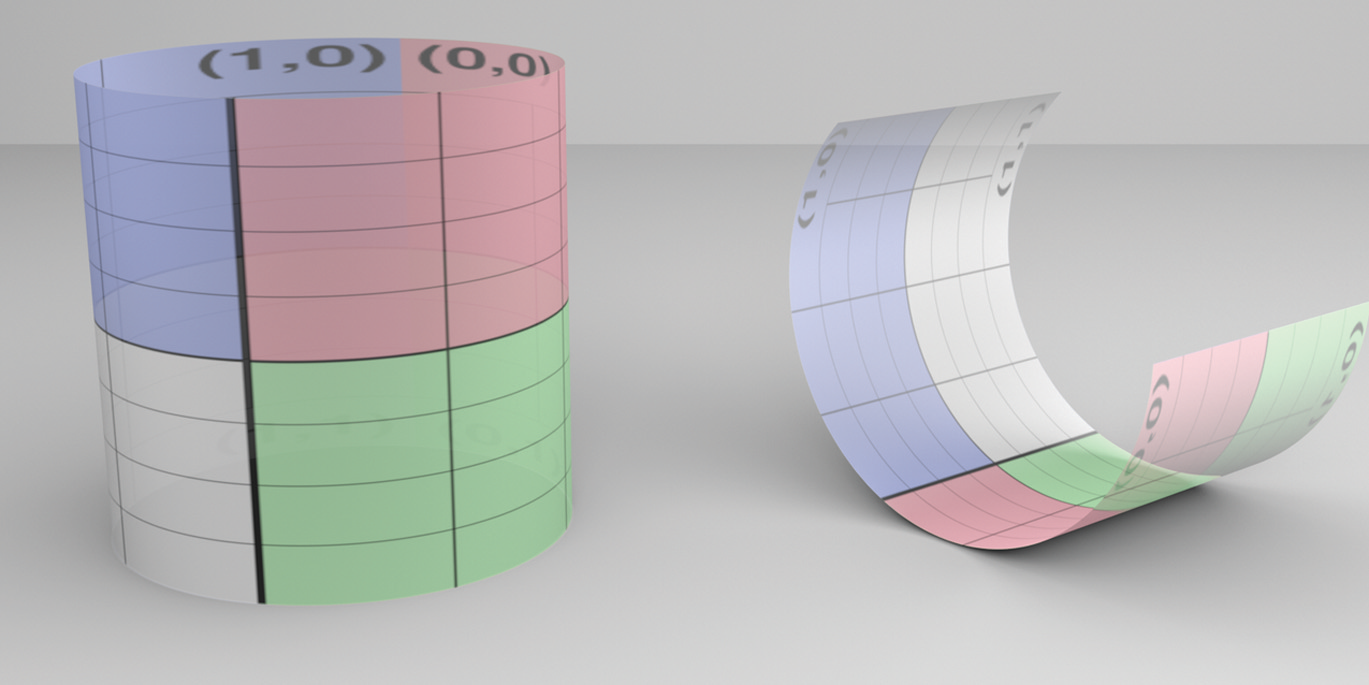
\includegraphics[width=\linewidth]{chap03/twocylinders.png}
    \caption{两个圆柱体。左边是完整圆柱体,右边是部分圆柱体。}
    \label{fig:3.7}
\end{figure}

\begin{lstlisting}
`\initcode{Cylinder Public Methods}{=}`
`\refvar{Cylinder}{}`(const `\refvar{Transform}{}` *ObjectToWorld, const `\refvar{Transform}{}` *WorldToObject,
         bool reverseOrientation, `\refvar{Float}{}` radius, `\refvar{Float}{}` zMin, `\refvar{Float}{}` zMax,
         `\refvar{Float}{}` phiMax)
    : `\refvar{Shape}{}`(ObjectToWorld, WorldToObject, reverseOrientation),
      `\refvar[Cylinder::radius]{radius}{}`(radius), `\refvar[Cylinder::zMin]{zMin}{}`(std::min(zMin, zMax)),
      `\refvar[Cylinder::zMax]{zMax}{}`(std::max(zMin, zMax)),
      `\refvar[Cylinder::phiMax]{phiMax}{}`(`\refvar{Radians}{}`(`\refvar{Clamp}{}`(phiMax, 0, 360))) { }
\end{lstlisting}
\begin{lstlisting}
`\initcode{Cylinder Private Data}{=}`
const `\refvar{Float}{}` `\initvar[Cylinder::radius]{radius}{}`, `\initvar[Cylinder::zMin]{zMin}{}`, `\initvar[Cylinder::zMax]{zMax}{}`, `\initvar[Cylinder::phiMax]{phiMax}{}`;
\end{lstlisting}

\subsection{边界}\label{sub:边界3}
像球那样,圆柱体边界方法用$z$的范围计算保守边界框但不考虑最大的$\varphi$。
\begin{lstlisting}
`\initcode{Cylinder Method Definitions}{=}\initnext{CylinderMethodDefinitions}`
`\refvar{Bounds3f}{}` `\refvar{Cylinder}{}`::`\initvar[Cylinder::ObjectBound]{\refvar{ObjectBound}{}}{}`() const {
    return `\refvar{Bounds3f}{}`(`\refvar{Point3f}{}`(-`\refvar[Cylinder::radius]{radius}{}`, -`\refvar[Cylinder::radius]{radius}{}`, `\refvar[Cylinder::zMin]{zMin}{}`),
                    `\refvar{Point3f}{}`( `\refvar[Cylinder::radius]{radius}{}`,  `\refvar[Cylinder::radius]{radius}{}`, `\refvar[Cylinder::zMax]{zMax}{}`));
}
\end{lstlisting}

\subsection{相交测试}\label{sub:相交测试3}
光线-圆柱体相交公式可以通过把射线方程代入圆柱体的隐式方程得到,和球体的情况一样。
以$z$轴为中心$r$为半径的无限长圆柱体的隐式方程为
\begin{align*}
    x^2+y^2-r^2=0\, .
\end{align*}
代入射线方程\refeq{2.3},我们有
\begin{align*}
    (o_x+td_x)^2+(o_y+td_y)^2=r^2\, .
\end{align*}
我们将其展开并求二次式方程$at^2+bt+c=0$的系数得
\begin{align*}
    a & =d_x^2+d_y^2\, ,      \\
    b & =2(d_xo_x+d_yo_y)\, , \\
    c & =o_x^2+o_y^2-r^2\, .
\end{align*}
\begin{lstlisting}
`\initcode{Compute quadratic cylinder coefficients}{=}`
`\refcode{Initialize EFloat ray coordinate values}{}`
`\refvar{EFloat}{}` a = dx * dx + dy * dy;
`\refvar{EFloat}{}` b = 2 * (dx * ox + dy * oy);
`\refvar{EFloat}{}` c = ox * ox + oy * oy - `\refvar{EFloat}{}`(`\refvar[Cylinder::radius]{radius}{}`) * `\refvar{EFloat}{}`(`\refvar[Cylinder::radius]{radius}{}`);
\end{lstlisting}

所有二次曲面形状求解二次方程的过程都一样,
所以下面会复用来自\refvar{Sphere}{}
相交方法的一些代码片。
\begin{lstlisting}
`\refcode{Cylinder Method Definitions}{+=}\lastnext{CylinderMethodDefinitions}`
bool `\refvar{Cylinder}{}`::`\initvar[Cylinder::Intersect]{\refvar[Shape::Intersect]{Intersect}{}}{}`(const `\refvar{Ray}{}` &r, `\refvar{EFloat}{}` *tHit,
        `\refvar{SurfaceInteraction}{}` *isect, bool testAlphaTexture) const {
    `\refvar{Float}{}` phi;
    `\refvar{Point3f}{}` pHit;
    `\refcode{Transform Ray to object space}{}`
    `\refcode{Compute quadratic cylinder coefficients}{}`
    `\refcode{Solve quadratic equation for t values}{}`
    `\refcode{Compute cylinder hit point and $\varphi$}{}`
    `\refcode{Test cylinder intersection against clipping parameters}{}`
    `\refcode{Find parametric representation of cylinder hit}{}`
    `\refcode{Compute error bounds for cylinder intersection}{}`
    `\refcode{Initialize SurfaceInteraction from parametric information}{}`
    `\refcode{Update tHit for quadric intersection}{}`
    return true;
}
\end{lstlisting}

像球体那样,这里的实现改进了计算的交点
以降低在计算射线方程中累积舍入误差的影响;见\refsub{定界交点误差}。
于是我们由圆柱体的参数化描述从$x$和$y$反解出$\varphi$;
最后所得结果与球体相同。
\begin{lstlisting}
`\initcode{Compute cylinder hit point and $\varphi$}{=}`
pHit = ray((`\refvar{Float}{}`)tShapeHit);
`\refcode{Refine cylinder intersection point}{}`
phi = std::atan2(pHit.y, pHit.x);
if (phi < 0) phi += 2 * `\refvar{Pi}{}`;
\end{lstlisting}

相交方法下一部分保证命中点在指定$z$范围内且能接受角度$\varphi$。
否则它就拒绝该命中点,并在之前还没尝试的前提下检查$t_1$——这和
\refvar{Sphere::Intersect}{()}
中的条件逻辑很像。
\begin{lstlisting}
`\initcode{Test cylinder intersection against clipping parameters}{=}`
if (pHit.z < `\refvar[Cylinder::zMin]{zMin}{}` || pHit.z > `\refvar[Cylinder::zMax]{zMax}{}` || phi > `\refvar[Cylinder::phiMax]{phiMax}{}`) {
    if (tShapeHit == t1) return false;
    tShapeHit = t1;
    if (t1.`\refvar{UpperBound}{}`() > ray.`\refvar{tMax}{}`) return false;
    `\refcode{Compute cylinder hit point and $\varphi$}{}`
    if (pHit.z < `\refvar[Cylinder::zMin]{zMin}{}` || pHit.z > `\refvar[Cylinder::zMax]{zMax}{}` || phi > `\refvar[Cylinder::phiMax]{phiMax}{}`)
        return false;
}
\end{lstlisting}

再次将$\varphi$缩放到0到1计算$u$值。
直接反解圆柱体参数方程的$z$值求得$v$参数坐标。
\begin{lstlisting}
`\initcode{Find parametric representation of cylinder hit}{=}`
`\refvar{Float}{}` u = phi / `\refvar[Cylinder::phiMax]{phiMax}{}`;
`\refvar{Float}{}` v = (pHit.z - `\refvar[Cylinder::zMin]{zMin}{}`) / (`\refvar[Cylinder::zMax]{zMax}{}` - `\refvar[Cylinder::zMin]{zMin}{}`);
`\refcode{Compute cylinder $\partial$p/$\partial$u and $\partial$p/$\partial$v}{}`
`\refcode{Compute cylinder $\partial$n/$\partial$u and $\partial$n/$\partial$v}{}`
\end{lstlisting}

圆柱体的偏导数很容易推导:
\begin{align*}
    \frac{\partial\bm p}{\partial u} & =(-\varphi_{\max}y,\varphi_{\max}x,0)\, , \\
    \frac{\partial\bm p}{\partial v} & =(0,0,z_{\max}-z_{\min})\, .
\end{align*}
\begin{lstlisting}
`\initcode{Compute cylinder $\partial$p/$\partial$u and $\partial$p/$\partial$v}{=}`
`\refvar{Vector3f}{}` dpdu(-`\refvar[Cylinder::phiMax]{phiMax}{}` * pHit.y, `\refvar[Cylinder::phiMax]{phiMax}{}` * pHit.x, 0);
`\refvar{Vector3f}{}` dpdv(0, 0, `\refvar[Cylinder::zMax]{zMax}{}` - `\refvar[Cylinder::zMin]{zMin}{}`);
\end{lstlisting}

我们又用Weingarten方程计算圆柱法线的参数化偏导数。
相关偏导数为:
\begin{align*}
    \frac{\partial^2\bm p}{\partial u^2}         & =-\varphi_{\max}^2(x,y,0)\, , \\
    \frac{\partial^2\bm p}{\partial u\partial v} & =(0,0,0)\, ,                  \\
    \frac{\partial^2\bm p}{\partial v^2}         & =(0,0,0)\, .
\end{align*}
\begin{lstlisting}
`\initcode{Compute cylinder $\partial$n/$\partial$u and $\partial$n/$\partial$v}{=}`
`\refvar{Vector3f}{}` d2Pduu = -`\refvar[Cylinder::phiMax]{phiMax}{}` * `\refvar[Cylinder::phiMax]{phiMax}{}` * `\refvar{Vector3f}{}`(pHit.x, pHit.y, 0);
`\refvar{Vector3f}{}` d2Pduv(0, 0, 0), d2Pdvv(0, 0, 0);
`\refcode{Compute coefficients for fundamental forms}{}`
`\refcode{Compute $\partial$n/$\partial$u and $\partial$n/$\partial$v from fundamental form coefficients}{}`
\end{lstlisting}

\subsection{表面积}\label{sub:表面积3}
圆柱体就是卷起来的矩形。如果你展开矩形,
其高是$z_{\max}-z_{\min}$,宽是$r\varphi_{\max}$:
\begin{lstlisting}
`\refcode{Cylinder Method Definitions}{+=}\lastnext{CylinderMethodDefinitions}`
`\refvar{Float}{}` `\refvar{Cylinder}{}`::`\initvar[Cylinder::Area]{\refvar[Shape::Area]{Area}{}}{}`() const {
    return (`\refvar[Cylinder::zMax]{zMax}{}` - `\refvar[Cylinder::zMin]{zMin}{}`) * `\refvar[Cylinder::radius]{radius}{}` * `\refvar[Cylinder::phiMax]{phiMax}{}`;
}
\end{lstlisting}

\section{圆盘}\label{sec:圆盘}

\keyindex{圆盘}{disk}{}是一种有趣的二次曲面,
因为它有特别简单的相交例程避免求解二次方程。

\section{其他二次曲面}\label{sec:其他二次曲面}

{\noindent\hfil$=========$\hfil{\color{red}{施工分割线}}\hfil$=========$\
\section{控制舍入误差}\label{sec:控制舍入误差}

\begin{remark}
    本节含有高级内容,第一次阅读时可以跳过。
\end{remark}

到目前为止,我们都是根据基于实数的理想化算术运算
纯粹地讨论光线-形状相交算法。该方法已经让我们走得很远了,
尽管有个重要事实是计算机只能表示有限的数量,
因此它实际上不能表示所有实数。
计算机用浮点数代替实数,它有固定的存储要求。
然而,因为结果可能无法在特定量的内存中表示,
每执行一次浮点运算就可能引入误差。

该误差的累积对相交测试的精度有些许影响。
首先,它可能造成完全错过有效的相交——
例如,一个精确值是正数的相交处$t$值算成了负的。
而且,算得的光线-形状交点可能在形状实际曲面的上面或下面。
这导致一个问题:当从算得的交点开始为阴影射线和反射光线追踪新光线时,
若射线端点在实际曲面之下,我们可能求得一次与曲面错误的再相交。
反之,若端点在曲面上面离得太远,阴影和反射可能会脱钩(见\reffig{3.39})。
\begin{figure}[htbp]
    \centering%LaTeX with PSTricks extensions
%%Creator: Inkscape 1.0.1 (3bc2e813f5, 2020-09-07)
%%Please note this file requires PSTricks extensions
\psset{xunit=.45pt,yunit=.45pt,runit=.45pt}
\begin{pspicture}(384.51998901,248.1499939)
{
\newrgbcolor{curcolor}{0 0 0}
\pscustom[linewidth=1,linecolor=curcolor,linestyle=dashed,dash=2]
{
\newpath
\moveto(219.8500061,133.36999512)
\lineto(190.47000122,209.74999237)
}
}
{
\newrgbcolor{curcolor}{0 0 0}
\pscustom[linewidth=1,linecolor=curcolor]
{
\newpath
\moveto(236.88000488,89.4099884)
\lineto(220.97000122,130.44999695)
}
}
{
\newrgbcolor{curcolor}{0 0 0}
\pscustom[linestyle=none,fillstyle=solid,fillcolor=curcolor]
{
\newpath
\moveto(227.88,127.8599939)
\lineto(221.2,129.8399939)
\lineto(217.61,123.8799939)
\lineto(218.04,137.9999939)
\closepath
}
}
{
\newrgbcolor{curcolor}{0.65098041 0.65098041 0.65098041}
\pscustom[linestyle=none,fillstyle=solid,fillcolor=curcolor]
{
\newpath
\moveto(226.19,128.8799939)
\lineto(218.51,136.7799939)
\lineto(220.98,130.4299939)
\closepath
}
}
{
\newrgbcolor{curcolor}{0.40000001 0.40000001 0.40000001}
\pscustom[linestyle=none,fillstyle=solid,fillcolor=curcolor]
{
\newpath
\moveto(218.18,125.7699939)
\lineto(218.51,136.7799939)
\lineto(220.98,130.4299939)
\closepath
}
}
{
\newrgbcolor{curcolor}{0 0 0}
\pscustom[linewidth=1,linecolor=curcolor,linestyle=dashed,dash=2]
{
\newpath
\moveto(304.55,139.9099939)
\lineto(261.9,24.0399939)
\lineto(236.11,91.4999939)
}
}
{
\newrgbcolor{curcolor}{0 0 0}
\pscustom[linewidth=1,linecolor=curcolor]
{
\newpath
\moveto(320.82998657,184.15999222)
\lineto(307.3500061,147.51999664)
}
}
{
\newrgbcolor{curcolor}{0 0 0}
\pscustom[linestyle=none,fillstyle=solid,fillcolor=curcolor]
{
\newpath
\moveto(303.88,154.0299939)
\lineto(307.57,148.1299939)
\lineto(314.21,150.2299939)
\lineto(304.55,139.9099939)
\closepath
}
}
{
\newrgbcolor{curcolor}{0.65098041 0.65098041 0.65098041}
\pscustom[linestyle=none,fillstyle=solid,fillcolor=curcolor]
{
\newpath
\moveto(304.47,152.1499939)
\lineto(305,141.1499939)
\lineto(307.35,147.5399939)
\closepath
}
}
{
\newrgbcolor{curcolor}{0.40000001 0.40000001 0.40000001}
\pscustom[linestyle=none,fillstyle=solid,fillcolor=curcolor]
{
\newpath
\moveto(312.54,149.1799939)
\lineto(305,141.1499939)
\lineto(307.35,147.5399939)
\closepath
}
}
{
\newrgbcolor{curcolor}{0 0 0}
\pscustom[linewidth=1,linecolor=curcolor,linestyle=dashed,dash=2]
{
\newpath
\moveto(132.72999573,89.11999512)
\lineto(188.08999634,207.56999207)
}
}
{
\newrgbcolor{curcolor}{0 0 0}
\pscustom[linewidth=1,linecolor=curcolor]
{
\newpath
\moveto(110,40.87998962)
\lineto(129.27999878,81.78999329)
}
}
{
\newrgbcolor{curcolor}{0 0 0}
\pscustom[linestyle=none,fillstyle=solid,fillcolor=curcolor]
{
\newpath
\moveto(132.16,74.9999939)
\lineto(129,81.1999939)
\lineto(122.21,79.6899939)
\lineto(132.73,89.1199939)
\closepath
}
}
{
\newrgbcolor{curcolor}{0.65098041 0.65098041 0.65098041}
\pscustom[linestyle=none,fillstyle=solid,fillcolor=curcolor]
{
\newpath
\moveto(131.74,76.9199939)
\lineto(132.18,87.9299939)
\lineto(129.27,81.7699939)
\closepath
}
}
{
\newrgbcolor{curcolor}{0.40000001 0.40000001 0.40000001}
\pscustom[linestyle=none,fillstyle=solid,fillcolor=curcolor]
{
\newpath
\moveto(123.96,80.5899939)
\lineto(132.18,87.9299939)
\lineto(129.27,81.7699939)
\closepath
}
}
{
\newrgbcolor{curcolor}{0 0 0}
\pscustom[linewidth=1,linecolor=curcolor,linestyle=dashed,dash=2]
{
\newpath
\moveto(73.42,114.5799939)
\lineto(102.58,25.0299939)
\lineto(110,40.8699939)
}
}
{
\newrgbcolor{curcolor}{0 0 0}
\pscustom[linewidth=1,linecolor=curcolor]
{
\newpath
\moveto(58.33000183,160.93999481)
\lineto(70.91000366,122.28999329)
}
}
{
\newrgbcolor{curcolor}{0 0 0}
\pscustom[linestyle=none,fillstyle=solid,fillcolor=curcolor]
{
\newpath
\moveto(64.16,125.2499939)
\lineto(70.71,122.8999939)
\lineto(74.63,128.6599939)
\lineto(73.42,114.5799939)
\closepath
}
}
{
\newrgbcolor{curcolor}{0.65098041 0.65098041 0.65098041}
\pscustom[linestyle=none,fillstyle=solid,fillcolor=curcolor]
{
\newpath
\moveto(65.78,124.1399939)
\lineto(73.02,115.8299939)
\lineto(70.91,122.3099939)
\closepath
}
}
{
\newrgbcolor{curcolor}{0.40000001 0.40000001 0.40000001}
\pscustom[linestyle=none,fillstyle=solid,fillcolor=curcolor]
{
\newpath
\moveto(73.96,126.7999939)
\lineto(73.02,115.8299939)
\lineto(70.91,122.3099939)
\closepath
}
}
{
\newrgbcolor{curcolor}{0.98823529 0.93333334 0.12941177}
\pscustom[linestyle=none,fillstyle=solid,fillcolor=curcolor]
{
\newpath
\moveto(195.71,230.6399939)
\lineto(194.14,220.9699939)
\lineto(199.09,229.4199939)
\lineto(195.76,220.1999939)
\lineto(202.18,227.6099939)
\lineto(197.22,219.1599939)
\lineto(204.89,225.2599939)
\lineto(198.46,217.8599939)
\lineto(207.12,222.4499939)
\lineto(199.44,216.3599939)
\lineto(208.79,219.2699939)
\lineto(200.13,214.6999939)
\lineto(209.86,215.8499939)
\lineto(200.5,212.9499939)
\lineto(210.28,212.2899939)
\lineto(200.54,211.1599939)
\lineto(210.03,208.7099939)
\lineto(200.25,209.3899939)
\lineto(209.13,205.2399939)
\lineto(199.64,207.6999939)
\lineto(207.61,201.9899939)
\lineto(198.74,206.1499939)
\lineto(205.52,199.0699939)
\lineto(197.56,204.7999939)
\lineto(202.93,196.5999939)
\lineto(196.16,203.6799939)
\lineto(199.92,194.6299939)
\lineto(194.57,202.8499939)
\lineto(196.61,193.2599939)
\lineto(192.86,202.3099939)
\lineto(193.1,192.5199939)
\lineto(191.08,202.1099939)
\lineto(189.51,192.4299939)
\lineto(189.29,202.2299939)
\lineto(185.97,192.9999939)
\lineto(187.55,202.6799939)
\lineto(182.6,194.2199939)
\lineto(185.93,203.4399939)
\lineto(179.5,196.0299939)
\lineto(184.47,204.4899939)
\lineto(176.8,198.3899939)
\lineto(183.23,205.7799939)
\lineto(174.57,201.1999939)
\lineto(182.25,207.2799939)
\lineto(172.89,204.3699939)
\lineto(181.56,208.9399939)
\lineto(171.83,207.7899939)
\lineto(181.19,210.6899939)
\lineto(171.41,211.3599939)
\lineto(181.15,212.4899939)
\lineto(171.66,214.9299939)
\lineto(181.44,214.2599939)
\lineto(172.56,218.4099939)
\lineto(182.04,215.9399939)
\lineto(174.08,221.6599939)
\lineto(182.95,217.4899939)
\lineto(176.17,224.5699939)
\lineto(184.13,218.8499939)
\lineto(178.76,227.0499939)
\lineto(185.53,219.9599939)
\lineto(181.77,229.0099939)
\lineto(187.12,220.7999939)
\lineto(185.08,230.3799939)
\lineto(188.83,221.3299939)
\lineto(188.59,231.1299939)
\lineto(190.61,221.5399939)
\lineto(192.17,231.2099939)
\lineto(192.4,221.4199939)
\closepath
}
}
{
\newrgbcolor{curcolor}{0 0 0}
\pscustom[linewidth=0.30000001,linecolor=curcolor]
{
\newpath
\moveto(195.71,230.6399939)
\lineto(194.14,220.9699939)
\lineto(199.09,229.4199939)
\lineto(195.76,220.1999939)
\lineto(202.18,227.6099939)
\lineto(197.22,219.1599939)
\lineto(204.89,225.2599939)
\lineto(198.46,217.8599939)
\lineto(207.12,222.4499939)
\lineto(199.44,216.3599939)
\lineto(208.79,219.2699939)
\lineto(200.13,214.6999939)
\lineto(209.86,215.8499939)
\lineto(200.5,212.9499939)
\lineto(210.28,212.2899939)
\lineto(200.54,211.1599939)
\lineto(210.03,208.7099939)
\lineto(200.25,209.3899939)
\lineto(209.13,205.2399939)
\lineto(199.64,207.6999939)
\lineto(207.61,201.9899939)
\lineto(198.74,206.1499939)
\lineto(205.52,199.0699939)
\lineto(197.56,204.7999939)
\lineto(202.93,196.5999939)
\lineto(196.16,203.6799939)
\lineto(199.92,194.6299939)
\lineto(194.57,202.8499939)
\lineto(196.61,193.2599939)
\lineto(192.86,202.3099939)
\lineto(193.1,192.5199939)
\lineto(191.08,202.1099939)
\lineto(189.51,192.4299939)
\lineto(189.29,202.2299939)
\lineto(185.97,192.9999939)
\lineto(187.55,202.6799939)
\lineto(182.6,194.2199939)
\lineto(185.93,203.4399939)
\lineto(179.5,196.0299939)
\lineto(184.47,204.4899939)
\lineto(176.8,198.3899939)
\lineto(183.23,205.7799939)
\lineto(174.57,201.1999939)
\lineto(182.25,207.2799939)
\lineto(172.89,204.3699939)
\lineto(181.56,208.9399939)
\lineto(171.83,207.7899939)
\lineto(181.19,210.6899939)
\lineto(171.41,211.3599939)
\lineto(181.15,212.4899939)
\lineto(171.66,214.9299939)
\lineto(181.44,214.2599939)
\lineto(172.56,218.4099939)
\lineto(182.04,215.9399939)
\lineto(174.08,221.6599939)
\lineto(182.95,217.4899939)
\lineto(176.17,224.5699939)
\lineto(184.13,218.8499939)
\lineto(178.76,227.0499939)
\lineto(185.53,219.9599939)
\lineto(181.77,229.0099939)
\lineto(187.12,220.7999939)
\lineto(185.08,230.3799939)
\lineto(188.83,221.3299939)
\lineto(188.59,231.1299939)
\lineto(190.61,221.5399939)
\lineto(192.17,231.2099939)
\lineto(192.4,221.4199939)
\closepath
}
}
{
\newrgbcolor{curcolor}{0 0 0}
\pscustom[linewidth=1,linecolor=curcolor]
{
\newpath
\moveto(36.70000076,54.98999023)
\lineto(345.42999268,54.98999023)
}
}
{
\newrgbcolor{curcolor}{0 0 0}
\pscustom[linestyle=none,fillstyle=solid,fillcolor=curcolor]
{
\newpath
\moveto(104.71000051,25.27999878)
\curveto(104.71000051,27.3737707)(102.17872502,28.4219561)(100.69838415,26.94161524)
\curveto(99.21804329,25.46127437)(100.26622869,22.92999887)(102.36000061,22.92999887)
\curveto(104.45377253,22.92999887)(105.50195793,25.46127437)(104.02161707,26.94161524)
\curveto(102.5412762,28.4219561)(100.01000071,27.3737707)(100.01000071,25.27999878)
\curveto(100.01000071,23.18622686)(102.5412762,22.13804146)(104.02161707,23.61838232)
\curveto(105.50195793,25.09872318)(104.45377253,27.62999868)(102.36000061,27.62999868)
\curveto(100.26622869,27.62999868)(99.21804329,25.09872318)(100.69838415,23.61838232)
\curveto(102.17872502,22.13804146)(104.71000051,23.18622686)(104.71000051,25.27999878)
\closepath
}
}
{
\newrgbcolor{curcolor}{0 0 0}
\pscustom[linewidth=1,linecolor=curcolor]
{
\newpath
\moveto(104.71000051,25.27999878)
\curveto(104.71000051,27.3737707)(102.17872502,28.4219561)(100.69838415,26.94161524)
\curveto(99.21804329,25.46127437)(100.26622869,22.92999887)(102.36000061,22.92999887)
\curveto(104.45377253,22.92999887)(105.50195793,25.46127437)(104.02161707,26.94161524)
\curveto(102.5412762,28.4219561)(100.01000071,27.3737707)(100.01000071,25.27999878)
\curveto(100.01000071,23.18622686)(102.5412762,22.13804146)(104.02161707,23.61838232)
\curveto(105.50195793,25.09872318)(104.45377253,27.62999868)(102.36000061,27.62999868)
\curveto(100.26622869,27.62999868)(99.21804329,25.09872318)(100.69838415,23.61838232)
\curveto(102.17872502,22.13804146)(104.71000051,23.18622686)(104.71000051,25.27999878)
\closepath
}
}
{
\newrgbcolor{curcolor}{0 0 0}
\pscustom[linestyle=none,fillstyle=solid,fillcolor=curcolor]
{
\newpath
\moveto(264.26000357,25.27999878)
\curveto(264.26000357,27.3737707)(261.72872807,28.4219561)(260.24838721,26.94161524)
\curveto(258.76804634,25.46127437)(259.81623174,22.92999887)(261.91000366,22.92999887)
\curveto(264.00377558,22.92999887)(265.05196098,25.46127437)(263.57162012,26.94161524)
\curveto(262.09127926,28.4219561)(259.56000376,27.3737707)(259.56000376,25.27999878)
\curveto(259.56000376,23.18622686)(262.09127926,22.13804146)(263.57162012,23.61838232)
\curveto(265.05196098,25.09872318)(264.00377558,27.62999868)(261.91000366,27.62999868)
\curveto(259.81623174,27.62999868)(258.76804634,25.09872318)(260.24838721,23.61838232)
\curveto(261.72872807,22.13804146)(264.26000357,23.18622686)(264.26000357,25.27999878)
\closepath
}
}
{
\newrgbcolor{curcolor}{0 0 0}
\pscustom[linewidth=1,linecolor=curcolor]
{
\newpath
\moveto(264.26000357,25.27999878)
\curveto(264.26000357,27.3737707)(261.72872807,28.4219561)(260.24838721,26.94161524)
\curveto(258.76804634,25.46127437)(259.81623174,22.92999887)(261.91000366,22.92999887)
\curveto(264.00377558,22.92999887)(265.05196098,25.46127437)(263.57162012,26.94161524)
\curveto(262.09127926,28.4219561)(259.56000376,27.3737707)(259.56000376,25.27999878)
\curveto(259.56000376,23.18622686)(262.09127926,22.13804146)(263.57162012,23.61838232)
\curveto(265.05196098,25.09872318)(264.00377558,27.62999868)(261.91000366,27.62999868)
\curveto(259.81623174,27.62999868)(258.76804634,25.09872318)(260.24838721,23.61838232)
\curveto(261.72872807,22.13804146)(264.26000357,23.18622686)(264.26000357,25.27999878)
\closepath
}
}
{
\newrgbcolor{curcolor}{0 0 0}
\pscustom[linewidth=1,linecolor=curcolor]
{
\newpath
\moveto(225.3999939,66.95999146)
\lineto(258.75,85.07998657)
}
}
{
\newrgbcolor{curcolor}{1 1 1}
\pscustom[linestyle=none,fillstyle=solid,fillcolor=curcolor]
{
\newpath
\moveto(111.72000265,38.94999695)
\curveto(111.72000265,41.04376887)(109.18872715,42.09195427)(107.70838629,40.6116134)
\curveto(106.22804543,39.13127254)(107.27623082,36.59999704)(109.37000275,36.59999704)
\curveto(111.46377467,36.59999704)(112.51196006,39.13127254)(111.0316192,40.6116134)
\curveto(109.55127834,42.09195427)(107.02000284,41.04376887)(107.02000284,38.94999695)
\curveto(107.02000284,36.85622503)(109.55127834,35.80803963)(111.0316192,37.28838049)
\curveto(112.51196006,38.76872135)(111.46377467,41.29999685)(109.37000275,41.29999685)
\curveto(107.27623082,41.29999685)(106.22804543,38.76872135)(107.70838629,37.28838049)
\curveto(109.18872715,35.80803963)(111.72000265,36.85622503)(111.72000265,38.94999695)
\closepath
}
}
{
\newrgbcolor{curcolor}{0 0 0}
\pscustom[linewidth=1,linecolor=curcolor]
{
\newpath
\moveto(111.72000265,38.94999695)
\curveto(111.72000265,41.04376887)(109.18872715,42.09195427)(107.70838629,40.6116134)
\curveto(106.22804543,39.13127254)(107.27623082,36.59999704)(109.37000275,36.59999704)
\curveto(111.46377467,36.59999704)(112.51196006,39.13127254)(111.0316192,40.6116134)
\curveto(109.55127834,42.09195427)(107.02000284,41.04376887)(107.02000284,38.94999695)
\curveto(107.02000284,36.85622503)(109.55127834,35.80803963)(111.0316192,37.28838049)
\curveto(112.51196006,38.76872135)(111.46377467,41.29999685)(109.37000275,41.29999685)
\curveto(107.27623082,41.29999685)(106.22804543,38.76872135)(107.70838629,37.28838049)
\curveto(109.18872715,35.80803963)(111.72000265,36.85622503)(111.72000265,38.94999695)
\closepath
}
}
{
\newrgbcolor{curcolor}{1 1 1}
\pscustom[linestyle=none,fillstyle=solid,fillcolor=curcolor]
{
\newpath
\moveto(240.07000113,87.34999084)
\curveto(240.07000113,89.44376277)(237.53872563,90.49194816)(236.05838476,89.0116073)
\curveto(234.5780439,87.53126644)(235.6262293,84.99999094)(237.72000122,84.99999094)
\curveto(239.81377314,84.99999094)(240.86195854,87.53126644)(239.38161768,89.0116073)
\curveto(237.90127682,90.49194816)(235.37000132,89.44376277)(235.37000132,87.34999084)
\curveto(235.37000132,85.25621892)(237.90127682,84.20803353)(239.38161768,85.68837439)
\curveto(240.86195854,87.16871525)(239.81377314,89.69999075)(237.72000122,89.69999075)
\curveto(235.6262293,89.69999075)(234.5780439,87.16871525)(236.05838476,85.68837439)
\curveto(237.53872563,84.20803353)(240.07000113,85.25621892)(240.07000113,87.34999084)
\closepath
}
}
{
\newrgbcolor{curcolor}{0 0 0}
\pscustom[linewidth=1,linecolor=curcolor]
{
\newpath
\moveto(240.07000113,87.34999084)
\curveto(240.07000113,89.44376277)(237.53872563,90.49194816)(236.05838476,89.0116073)
\curveto(234.5780439,87.53126644)(235.6262293,84.99999094)(237.72000122,84.99999094)
\curveto(239.81377314,84.99999094)(240.86195854,87.53126644)(239.38161768,89.0116073)
\curveto(237.90127682,90.49194816)(235.37000132,89.44376277)(235.37000132,87.34999084)
\curveto(235.37000132,85.25621892)(237.90127682,84.20803353)(239.38161768,85.68837439)
\curveto(240.86195854,87.16871525)(239.81377314,89.69999075)(237.72000122,89.69999075)
\curveto(235.6262293,89.69999075)(234.5780439,87.16871525)(236.05838476,85.68837439)
\curveto(237.53872563,84.20803353)(240.07000113,85.25621892)(240.07000113,87.34999084)
\closepath
}
}
\end{pspicture}

    \caption{可能在图像中造成可见错误的舍入误差问题几何设置。
        左边的入射光线与曲面相交。在左图中,算得的交点(黑圆圈)略低于曲面
        且阴影射线端点过低的“epsilon”偏移可能导致错误的自相交,
        因为阴影射线端点(白圆圈)仍在曲面之下;因此错误地认定光源被遮挡了。
        右图中,太高的“epsilon”导致错过了有效相交,
        因为射线端点通过了遮挡面。}
    \label{fig:3.39}
\end{figure}

在光线追踪中解决该问题的典型实践是将生成的射线偏移固定的“射线epsilon”值
\sidenote{译者注:epsilon即希腊字母$\epsilon$。},
忽略沿射线$\bm p+t\bm d$比某个$t_{\min}$还近的任何相交。
\reffig{3.40}展示了为什么该方法需要很高的$t_{\min}$值才能高效工作:
如果生成的射线相对于曲面非常倾斜,
则在离射线很远处可能会发生错误的射线相交。
不幸的是,大的$t_{\min}$值会造成射线端点相对远离原始交点,
这又反过来造成错过附近的有效相交,导致阴影和反射丢失细节。
\begin{figure}[htbp]
    \centering%LaTeX with PSTricks extensions
%%Creator: Inkscape 1.0.1 (3bc2e813f5, 2020-09-07)
%%Please note this file requires PSTricks extensions
\psset{xunit=.5pt,yunit=.5pt,runit=.5pt}
\begin{pspicture}(311.58999634,120.58000183)
{
\newrgbcolor{curcolor}{0 0 0}
\pscustom[linewidth=1,linecolor=curcolor]
{
\newpath
\moveto(0,32.56000519)
\lineto(308.73001099,32.56000519)
}
}
{
\newrgbcolor{curcolor}{0 0 0}
\pscustom[linestyle=none,fillstyle=solid,fillcolor=curcolor]
{
\newpath
\moveto(68.00000143,2.84999847)
\curveto(68.00000143,4.9437704)(65.46872593,5.99195579)(63.98838507,4.51161493)
\curveto(62.50804421,3.03127407)(63.5562296,0.49999857)(65.65000153,0.49999857)
\curveto(67.74377345,0.49999857)(68.79195884,3.03127407)(67.31161798,4.51161493)
\curveto(65.83127712,5.99195579)(63.30000162,4.9437704)(63.30000162,2.84999847)
\curveto(63.30000162,0.75622655)(65.83127712,-0.29195884)(67.31161798,1.18838202)
\curveto(68.79195884,2.66872288)(67.74377345,5.19999838)(65.65000153,5.19999838)
\curveto(63.5562296,5.19999838)(62.50804421,2.66872288)(63.98838507,1.18838202)
\curveto(65.46872593,-0.29195884)(68.00000143,0.75622655)(68.00000143,2.84999847)
\closepath
}
}
{
\newrgbcolor{curcolor}{0 0 0}
\pscustom[linewidth=1,linecolor=curcolor]
{
\newpath
\moveto(68.00000143,2.84999847)
\curveto(68.00000143,4.9437704)(65.46872593,5.99195579)(63.98838507,4.51161493)
\curveto(62.50804421,3.03127407)(63.5562296,0.49999857)(65.65000153,0.49999857)
\curveto(67.74377345,0.49999857)(68.79195884,3.03127407)(67.31161798,4.51161493)
\curveto(65.83127712,5.99195579)(63.30000162,4.9437704)(63.30000162,2.84999847)
\curveto(63.30000162,0.75622655)(65.83127712,-0.29195884)(67.31161798,1.18838202)
\curveto(68.79195884,2.66872288)(67.74377345,5.19999838)(65.65000153,5.19999838)
\curveto(63.5562296,5.19999838)(62.50804421,2.66872288)(63.98838507,1.18838202)
\curveto(65.46872593,-0.29195884)(68.00000143,0.75622655)(68.00000143,2.84999847)
\closepath
}
}
{
\newrgbcolor{curcolor}{0 0 0}
\pscustom[linewidth=1,linecolor=curcolor,linestyle=dashed,dash=2]
{
\newpath
\moveto(129.72999573,15.99000549)
\lineto(311.48999023,53.27999878)
}
}
{
\newrgbcolor{curcolor}{0 0 0}
\pscustom[linewidth=1,linecolor=curcolor,linestyle=dashed,dash=2]
{
\newpath
\moveto(120.30999756,14.06000519)
\lineto(129.72999573,15.99000549)
}
}
{
\newrgbcolor{curcolor}{0 0 0}
\pscustom[linewidth=1,linecolor=curcolor]
{
\newpath
\moveto(65.65000153,2.84999847)
\lineto(112.37999725,12.43000031)
}
}
{
\newrgbcolor{curcolor}{0 0 0}
\pscustom[linestyle=none,fillstyle=solid,fillcolor=curcolor]
{
\newpath
\moveto(108.67,6.05000183)
\lineto(111.74,12.30000183)
\lineto(106.46,16.84000183)
\lineto(120.31,14.06000183)
\closepath
}
}
{
\newrgbcolor{curcolor}{0.65098041 0.65098041 0.65098041}
\pscustom[linestyle=none,fillstyle=solid,fillcolor=curcolor]
{
\newpath
\moveto(109.96,7.55000183)
\lineto(119.03,13.80000183)
\lineto(112.36,12.43000183)
\closepath
}
}
{
\newrgbcolor{curcolor}{0.40000001 0.40000001 0.40000001}
\pscustom[linestyle=none,fillstyle=solid,fillcolor=curcolor]
{
\newpath
\moveto(108.23,15.97000183)
\lineto(119.03,13.80000183)
\lineto(112.36,12.43000183)
\closepath
}
}
{
\newrgbcolor{curcolor}{0 0 0}
\pscustom[linewidth=1,linecolor=curcolor,linestyle=dashed,dash=2]
{
\newpath
\moveto(43.90000153,75.87000275)
\lineto(65.65000153,2.84999847)
}
}
{
\newrgbcolor{curcolor}{0 0 0}
\pscustom[linewidth=1,linecolor=curcolor]
{
\newpath
\moveto(30.62000084,120.44000183)
\lineto(41.58000183,83.6400032)
}
}
{
\newrgbcolor{curcolor}{0 0 0}
\pscustom[linestyle=none,fillstyle=solid,fillcolor=curcolor]
{
\newpath
\moveto(34.91,86.77000183)
\lineto(41.4,84.26000183)
\lineto(45.46,89.92000183)
\lineto(43.9,75.87000183)
\closepath
}
}
{
\newrgbcolor{curcolor}{0.65098041 0.65098041 0.65098041}
\pscustom[linestyle=none,fillstyle=solid,fillcolor=curcolor]
{
\newpath
\moveto(36.5,85.62000183)
\lineto(43.52,77.13000183)
\lineto(41.58,83.66000183)
\closepath
}
}
{
\newrgbcolor{curcolor}{0.40000001 0.40000001 0.40000001}
\pscustom[linestyle=none,fillstyle=solid,fillcolor=curcolor]
{
\newpath
\moveto(44.74,88.08000183)
\lineto(43.52,77.13000183)
\lineto(41.58,83.66000183)
\closepath
}
}
{
\newrgbcolor{curcolor}{1 1 1}
\pscustom[linestyle=none,fillstyle=solid,fillcolor=curcolor]
{
\newpath
\moveto(212.12000418,32.54000092)
\curveto(212.12000418,34.63377284)(209.58872868,35.68195823)(208.10838782,34.20161737)
\curveto(206.62804695,32.72127651)(207.67623235,30.19000101)(209.77000427,30.19000101)
\curveto(211.8637762,30.19000101)(212.91196159,32.72127651)(211.43162073,34.20161737)
\curveto(209.95127987,35.68195823)(207.42000437,34.63377284)(207.42000437,32.54000092)
\curveto(207.42000437,30.44622899)(209.95127987,29.3980436)(211.43162073,30.87838446)
\curveto(212.91196159,32.35872532)(211.8637762,34.89000082)(209.77000427,34.89000082)
\curveto(207.67623235,34.89000082)(206.62804695,32.35872532)(208.10838782,30.87838446)
\curveto(209.58872868,29.3980436)(212.12000418,30.44622899)(212.12000418,32.54000092)
\closepath
}
}
{
\newrgbcolor{curcolor}{0 0 0}
\pscustom[linewidth=1,linecolor=curcolor]
{
\newpath
\moveto(212.12000418,32.54000092)
\curveto(212.12000418,34.63377284)(209.58872868,35.68195823)(208.10838782,34.20161737)
\curveto(206.62804695,32.72127651)(207.67623235,30.19000101)(209.77000427,30.19000101)
\curveto(211.8637762,30.19000101)(212.91196159,32.72127651)(211.43162073,34.20161737)
\curveto(209.95127987,35.68195823)(207.42000437,34.63377284)(207.42000437,32.54000092)
\curveto(207.42000437,30.44622899)(209.95127987,29.3980436)(211.43162073,30.87838446)
\curveto(212.91196159,32.35872532)(211.8637762,34.89000082)(209.77000427,34.89000082)
\curveto(207.67623235,34.89000082)(206.62804695,32.35872532)(208.10838782,30.87838446)
\curveto(209.58872868,29.3980436)(212.12000418,30.44622899)(212.12000418,32.54000092)
\closepath
}
}
\end{pspicture}

    \caption{如果算得的交点(实心圆)低于曲面且生成的射线是斜的,
        在与射线端点有一定距离的地方可能会发生错误的再相交(空心圆)。
        如果用沿射线的最小$t$值消除附近的相交,
        需要相对大的$t_{\min}$才能处理好倾斜射线。}
    \label{fig:3.40}
\end{figure}

本节中,我们将介绍浮点算术基本思想并描述分析浮点计算误差的技术。
然后我们将这些方法用于本章之前介绍的光线-形状算法
并展示怎样计算带有有界误差的光线交点。
这将允许我们保守地定位射线端点,这样就永远不会求得错误的自相交,
而又保留了与实际交点极其接近的射线端点使得错误脱靶被最小化。
反过来也不需要额外的“射线epsilon”值。

\subsection{浮点算术}\label{sub:浮点算术}
计算必须在容纳于有限量内存的数字的有限表示上执行;
计算机上无法表示实数的无限集合。
一种这样的有限表示是定点,例如给定一个16位整数,
有人可能通过除以256将其映射为正实数。
这允许我们表示值之间具有相等间距$\displaystyle\frac{1}{256}$的
范围$\displaystyle\left[0,\frac{65535}{256}\right]=\left[0,255+\frac{255}{256}\right]$。
\keyindex{定点数}{fixed-point number}{}可以用整数算术运算高效实现
(该特性使其在早期不支持浮点计算的个人计算机上很流行),
但是它们受制于许多缺点:其中,它们能表示的最大数字是受限的,
且不能精确表示非常小的接近于零的数。

计算机上实数的另一种表示是\keyindex{浮点数}{floating-point number}{}。
它用\keyindex{符号}{sign}{}、\keyindex{有效数字}{significand}{}\footnote{单词“\protect\keyindex{尾数}{mantissa}{}”
    常用来代替“有效数字”,但浮点纯粹主义者注意到“尾数”在对数上下文中
    有不同含义而因此更偏爱“有效数字”。这里我们遵循该用法。}和\keyindex{指数}{exponent}{}表示数字:
本质上和\keyindex{科学计数法}{scientific notation}{}相同但用固定数量的数字表示有效数字和指数。
(下文中,我们将只讨论以2为底的数字。)
这种表示能够用固定数量的存储对极大范围的数字进行表示和执行计算。

用浮点算术的程序员通常知道浮点是不精确的;
有时这种看法导致了浮点算术是不可预测的观念。
本节中我们将看到浮点算术有精心设计的基础反而
能计算特定计算中引入误差的保守边界。
对于光线追踪计算,该误差常意外地小。

现代CPU和GPU几乎都基于电气与电子工程师协会
\sidenote{译者注:即Institute of Electrical and Electronics Engineers (IEEE),
    是电气工程与电子工程以及相关学科的专业协会,成立于1963年1月,总部在美国纽约。
    其范围已经扩展到电气、电子、通信、计算机工程、计算机科学与信息技术等诸多领域,
    是世界上最大的技术专业组织。}
颁布的标准\parencite*{10.1109/IEEESTD.1985.82928,10.1109/IEEESTD.2008.4610935}实现浮点算术模型。
(今后我们说的浮点特指IEEE 754规定的32位浮点数。)
IEEE 754技术标准规定了内存中浮点数的格式以及
精度和浮点计算舍入的特定规则;
正是这些规则使得能对给定浮点值中出现的误差进行严格推导。

\subsubsection*{浮点表示}
IEEE标准规定32位浮点用1位符号、8位指数和23位有效数字表示。
用了8位的指数$e$范围为从0到255;
实际用的指数$e_{\mathrm{b}}$是通过偏置$e$算得的:
\begin{align*}
    e_{\mathrm{b}}=e-127\, .
\end{align*}

当存储\keyindex{规范化的}{normalized}{}浮点值时有效数字实际有24位精度。
当有效数字和指数表示规范化的数字时,有效数字中没有前导零。
在\keyindex{二进制}{binary}{}中,这意味着有效数字开头的数字必须是一;
反过来,没必要显式存储该值。
因此,隐式前导的1位和编码有效数字小数部分的23位给出了总共24位的精度。

给定符号$s=\pm 1$、有效数字$m$和指数$e$,相应的浮点值为
\begin{align*}
    s\times 1.m\times2^{e-127}\, .
\end{align*}

例如,浮点数6.5可以通过规范化的有效数字写作$1.101_2\times2^2$,
其中下标2表示以2为底的值\sidenote{译者注:即二进制。}
(如果非整数的二进制数不够直观,可以注意
小数点右边第一个数表示$2^{-1}$,以此类推)。
因此,我们有
\begin{align*}
    (1\times2^0+1\times2^{-1}+0\times2^{-2}+1\times2^{-3})\times2^2=1.625\times2^2=6.5\, .
\end{align*}
$e_{\mathrm{b}}=2$,所以$e=129=10000001_2$且$m=10100000000000000000000_2$。

浮点在内存中的布局是符号位在32位值的最高位
(负号用一位编码),然后是指数和有效数字。
因此,对于值6.5其内存中的二进制表示是
\begin{align*}
    0\ 10000001\ 10100000000000000000000=40\mathrm{d}00000_{16}\, .
\end{align*}

同样,浮点值1.0有$m=0\ldots0_2$和$e_{\mathrm{b}}=0$,所以$e=127=01111111_2$,它的二进制表示为
\begin{align*}
    0\ 01111111\ 00000000000000000000000=3\mathrm{f}800000_{16}\, .
\end{align*}

该\keyindex{十六进制}{hexadecimal}{}值值得记住,因为调试时它常出现于内存转储。

该表示隐含了整个范围内两个相邻的二的幂次之间
可表示的浮点数之间的间隔是均匀的(它对应于有效数字位增一)。
在范围$[2^e,2^{e+1})$内,间隔为
\begin{align}\label{eq:3.6}
    2^{e-23}\, .
\end{align}
因此对1和2之间的浮点数,$e=0$,
浮点值间的间隔为$2^{-23}\approx1.19209\times10^{-7}$。
该间隔也称为\keyindex{最后一位上的单位值}{unit in last place}{}(ulp)\sidenote{译者注:也叫“最小精度单位”。}的大小;
注意一个ulp的大小由相应浮点值决定——更大的数的ulp比更小的数的ulp相对更大。

按我们目前描述的表示是不可能恰好将零表示为浮点数的。
这事显然不可接受,所以最小指数$e=0$,
或说$e_{\mathrm{b}}=-127$,被留出来特殊对待。
对于该指数,浮点值解释为有效数字中没有隐式前导一位,
这意味全零位的有效数字会得到
\begin{align*}
    s\times0.0\ldots0_2\times2^{-127}=0\, .
\end{align*}

去掉有效数字前导一位也能表示\keyindex{非规范化的}{denormalized}{}数:
如果总是出现前导一\sidenote{译者注:我完善了该式。},则最小的32位浮点是
\begin{align*}
    1.{\underbrace{0\ldots0}_{\text{23个0}}}\ _2\times2^{-127}\approx5.8774718\times10^{-39}\, .
\end{align*}
没有前导一位\sidenote{译者注:我完善了该式;如果你难以理解为何指数变成了$2^{-126}$,
也可以等价地看作$\underbrace{0.0\ldots0}_{22\text{个}0}1_2\times2^{-127}=2^{-22}\times2^{-127}$。},最小值是
\begin{align*}
    0.\underbrace{0\ldots0}_{\text{22个0}}1_2\times2^{-126}=2^{-23}\times2^{-126}\approx1.4012985\times10^{-45}\, .
\end{align*}

有了表示这些小值的能力可以避免需要将非常小的数舍入为零。

注意该表示同时有“正”和“负”零值。
该细节对程序员大多是透明的。
例如,标准保证了比较{\ttfamily -0.0 == 0.0}为真,
即使这两值在内存中的表示不同。

最大指数,$e=255$,也保留作特殊对待。
因此,可以表示的最大规范化浮点值有$e=254$(或$e_{\mathrm{b}}=127$)且约为\sidenote{译者注:我完善了该式。}
\begin{align*}
    1.{\underbrace{1\ldots1}_{\text{23个1}}}\ _2\times2^{127}=(2-2^{-23})\times2^{127}\approx3.402823\times10^{38}\, .
\end{align*}

对于$e=255$,若有效数字位全是零,则该值依据符号位对应正或负无穷。
例如,在浮点中执行像1/0的计算会得到无穷值。
对无穷的算术运算得到无穷。
比较时,正无穷大于任何非无穷值,负无穷类似。

常数\refvar{MaxFloat}{}和\refvar{Infinity}{}分别初始化为可表示的最大和“无穷”浮点值。
我们令其可在单独的常数中获取,这样使用这些值的代码
就不需要用唠叨的C++标准库调用来获取它们的值了。
\begin{lstlisting}
`\initcode{Global Constants}{=}\initnext{GlobalConstants}`
static constexpr `\refvar{Float}{}` `\initvar{MaxFloat}{}` = std::numeric_limits<`\refvar{Float}{}`>::max();
static constexpr `\refvar{Float}{}` `\initvar{Infinity}{}` = std::numeric_limits<`\refvar{Float}{}`>::infinity();
\end{lstlisting}

对于$e=255$,非零有效数字位对应
特殊的NaN值\sidenote{译者注:原文误写为$e_b=255$,已修正。},
它由诸如取负数平方根或尝试计算0/0的运算得到。
NaN随计算传播:\keyindex{运算对象}{operand}{}之一
为NaN本身的任何算术运算总是返回NaN。
因此,如果NaN出现于一长串计算中,
我们就知道该方式中的某处出错了。
在调试构建中,pbrt有许多\refvar{Assert}{()}语句检查NaN值,
因为我们几乎从不希望它们出现在事件的常规过程中。
任何与NaN值的比较返回假;
因此检查{\ttfamily !(x == x)}用来检查值是否不是数字
\footnote{这是编译器不得对包含浮点值的表达式执行
看似明显且安全的代数简化的少数几个地方之一——
这个特别的比较不得简化为{\ttfamily false}。
启用编译器的“快速数学”或“执行不安全的数学优化”标志
可能会允许执行这些优化。但是错误行为可能引入pbrt中。}。
为了清楚起见,我们用C++标准库函数{\ttfamily std::isnan()}来检查NaN值。

\subsubsection*{实用例程}
对于某些底层运算,能将浮点值解释为其组成位以及将表示浮点值的数位
转换为实际的{\ttfamily float}或{\ttfamily double}很有用。

一个自然的方法是取指向要转换的值的指针并将其强制转换为另一类型:
{\ttfamily\newline\noindent
float f = ...;\newline\noindent
uint32\_t bits = *((uint32\_t *)\&f);\newline
}
然而,现代版本的C++规定将一种{\ttfamily float}指针强制转换为
不同类型{\ttfamily uint32\_t}是非法的
(该限制允许编译器在分析两个指针是否可能指向
同一内存位置时进行更激进的优化,禁止在寄存器中保存值)。

另一常见方法是对两类元素使用{\ttfamily union},赋予一种类型并按另一种读取:
{\ttfamily\newline\noindent
union FloatBits \{\newline\noindent
\indent float f;\newline\noindent
\indent uint32\_t ui;\newline\noindent
\};\newline\noindent
FloatBits fb;\newline\noindent
fb.f = ...;\newline\noindent
uint32\_t bits = fb.ui;
}

这也是非法的:C++标准说从{\ttfamily union}读取和最后一次赋值时不同的元素是未定义行为。

可以用{\ttfamily memcpy()}将指向源类型的指针复制到指向目标类型的指针来正确执行这些转换。
\begin{lstlisting}
`\initcode{Global Inline Functions}{=}\initnext{GlobalInlineFunctions}`
inline uint32_t `\initvar{FloatToBits}{}`(float f) {
    uint32_t ui;
    memcpy(&ui, &f, sizeof(float));
    return ui;
}
\end{lstlisting}
\begin{lstlisting}
`\refcode{Global Inline Functions}{+=}\lastnext{GlobalInlineFunctions}`
inline float `\initvar{BitsToFloat}{}`(uint32_t ui) {
    float f;
    memcpy(&f, &ui, sizeof(uint32_t));
    return f;
}
\end{lstlisting}

尽管调用函数{\ttfamily memcpy()}以避免这些问题可能看起来太昂贵了,
但实际中好的编译器会将其变为无操作而只是将寄存器或内存中的内容重新解释为另一类型
(pbrt中还有这些函数在{\ttfamily double}和{\ttfamily uint64\_t}之间
转换的类似版本,所以这里就不介绍了)。

这些转换可用于实现函数即把浮点值向上或向下调整到相邻更大或更小的可表示浮点值
\footnote{这些函数等价于{\ttfamily std::nextafter(v, Infinity)}和{\ttfamily std::nextafter(v, -Infinity)}但更加高效,
因为它们不负责处理NaN值或浮点信号异常。}。
它们对我们接下来的代码中需要的某些保守的舍入操作很有用。
多亏浮点在内存中表示的特殊性,这些操作很高效。
\begin{lstlisting}
`\refcode{Global Inline Functions}{+=}\lastnext{GlobalInlineFunctions}`
inline float `\initvar{NextFloatUp}{}`(float v) {
    `\refcode{Handle infinity and negative zero for NextFloatUp()}{}`
    `\refcode{Advance v to next higher float}{}`
}
\end{lstlisting}

有两种重要的特殊情况:如果{\ttfamily v}为正无穷,则该函数就返回没变的{\ttfamily v}。
在继续执行有效数字的代码之前让负零向前跳到正零。
这一步必须显式处理,因为-0.0和0.0的位模式不相邻。
\begin{lstlisting}
`\initcode{Handle infinity and negative zero for NextFloatUp()}{=}`
if (std::isinf(v) && v > 0.)
    return v;
if (v == -0.f)
    v = 0.f;
\end{lstlisting}

概念上,给定一浮点值,我们想对有效数字增加一,
如果结果\keyindex{溢出}{overflow}{},
则有效数字重置为零且指数增加一。
意外的是对浮点在内存中的整数表示加一实现了这点:
因为指数在有效数字之上的高位,所以如果有效数字全是一,
则有效数字低位加一会将一一路带到指数去,
否则就在当前指数下推进到相邻更大的有效数字。
还要注意当增加最大可表示的有限浮点值数位表示时,
会得到正的浮点无穷数位模式。

对于负值,从数位表示减一类似地推进到相邻值。
\begin{lstlisting}
`\initcode{Advance v to next higher float}{=}`
uint32_t ui = `\refvar{FloatToBits}{}`(v);
if (v >= 0) ++ui;
else        --ui;
return `\refvar{BitsToFloat}{}`(ui);
\end{lstlisting}

这里没有介绍函数{\initvar{NextFloatDown}{()}}了,
它遵循相同的逻辑但高效地取反。
pbrt也提供了这些函数的{\ttfamily double}版本。

\subsubsection*{算术运算}
IEEE 754提供了关于浮点算术的重要保证:
具体而言,它保证了加法、减法、乘法、除法和平方根
在相同输入下给出相同结果且这些结果的浮点数最接近于
在无限精度算术下执行底层计算的结果
\footnote{IEEE浮点允许用户选一种数字舍入模式,
    但我们这里假设用默认的——舍入到最近的偶数。}。
值得注意的是这在有限精度数字计算机上是完全可能的;
IEEE 754的成就之一是证明了这种级别的精度是可能的且
能在硬件上很高效地实现。

用圆圈运算符表示浮点算术运算符,用sqrt表示浮点平方根,
这些精度保证可以写作:
\begin{align}
    a\oplus b        & =\mathrm{round}(a+b)\, ,\nonumber      \\
    a\ominus b       & =\mathrm{round}(a-b)\, ,\nonumber      \\
    a\otimes b       & =\mathrm{round}(a*b)\, ,\label{eq:3.7} \\
    a\oslash b       & =\mathrm{round}(a/b)\, ,\nonumber      \\
    \mathrm{sqrt}(a) & =\mathrm{round}(\sqrt{a})\, ,\nonumber
\end{align}
其中$\mathrm{round}(x)$表示将实数舍入到最接近的浮点值的结果。

舍入误差的界可以表示为实数区间:例如
对于加法,我们可以说舍入的结果在与某个$\epsilon$有关的区间内
\begin{align}
    a\oplus b & =\mathrm{round}(a+b)\in(a+b)(1\pm\epsilon)\nonumber \\
              & =[(a+b)(1-\epsilon),(a+b)(1+\epsilon)]\, ,
    \label{eq:3.8}
\end{align}
该舍入引入的误差量不超过在$a+b$处的浮点间隔的一半——
如果它超过浮点间隔的一半,则它会以更小误差舍入到另一个不同的浮点数(\reffig{3.41})。
\begin{figure}[htbp]
    \centering%LaTeX with PSTricks extensions
%%Creator: Inkscape 1.0.1 (3bc2e813f5, 2020-09-07)
%%Please note this file requires PSTricks extensions
\psset{xunit=.5pt,yunit=.5pt,runit=.5pt}
\begin{pspicture}(290.97000122,48.74321747)
{
\newrgbcolor{curcolor}{0 0 0}
\pscustom[linestyle=none,fillstyle=solid,fillcolor=curcolor]
{
\newpath
\moveto(175.22998953,38.20321655)
\curveto(175.22998953,40.29698848)(172.69871403,41.34517387)(171.21837317,39.86483301)
\curveto(169.73803231,38.38449215)(170.7862177,35.85321665)(172.87998962,35.85321665)
\curveto(174.97376155,35.85321665)(176.02194694,38.38449215)(174.54160608,39.86483301)
\curveto(173.06126522,41.34517387)(170.52998972,40.29698848)(170.52998972,38.20321655)
\curveto(170.52998972,36.10944463)(173.06126522,35.06125923)(174.54160608,36.5416001)
\curveto(176.02194694,38.02194096)(174.97376155,40.55321646)(172.87998962,40.55321646)
\curveto(170.7862177,40.55321646)(169.73803231,38.02194096)(171.21837317,36.5416001)
\curveto(172.69871403,35.06125923)(175.22998953,36.10944463)(175.22998953,38.20321655)
\closepath
}
}
{
\newrgbcolor{curcolor}{0 0 0}
\pscustom[linewidth=1,linecolor=curcolor]
{
\newpath
\moveto(175.22998953,38.20321655)
\curveto(175.22998953,40.29698848)(172.69871403,41.34517387)(171.21837317,39.86483301)
\curveto(169.73803231,38.38449215)(170.7862177,35.85321665)(172.87998962,35.85321665)
\curveto(174.97376155,35.85321665)(176.02194694,38.38449215)(174.54160608,39.86483301)
\curveto(173.06126522,41.34517387)(170.52998972,40.29698848)(170.52998972,38.20321655)
\curveto(170.52998972,36.10944463)(173.06126522,35.06125923)(174.54160608,36.5416001)
\curveto(176.02194694,38.02194096)(174.97376155,40.55321646)(172.87998962,40.55321646)
\curveto(170.7862177,40.55321646)(169.73803231,38.02194096)(171.21837317,36.5416001)
\curveto(172.69871403,35.06125923)(175.22998953,36.10944463)(175.22998953,38.20321655)
\closepath
}
}
{
\newrgbcolor{curcolor}{0 0 0}
\pscustom[linewidth=1,linecolor=curcolor]
{
\newpath
\moveto(289.54998779,38.20321655)
\lineto(1.5,38.20321655)
}
}
{
\newrgbcolor{curcolor}{0 0 0}
\pscustom[linewidth=1,linecolor=curcolor]
{
\newpath
\moveto(1.5,47.74321747)
\lineto(1.5,28.65321732)
}
}
{
\newrgbcolor{curcolor}{0 0 0}
\pscustom[linewidth=1,linecolor=curcolor]
{
\newpath
\moveto(73.48999786,47.74321747)
\lineto(73.48999786,28.65321732)
}
}
{
\newrgbcolor{curcolor}{0 0 0}
\pscustom[linewidth=1,linecolor=curcolor]
{
\newpath
\moveto(289.47000122,47.74321747)
\lineto(289.47000122,28.65321732)
}
}
{
\newrgbcolor{curcolor}{0 0 0}
\pscustom[linewidth=1,linecolor=curcolor]
{
\newpath
\moveto(145.47999573,47.74321747)
\lineto(145.47999573,28.65321732)
}
}
{
\newrgbcolor{curcolor}{0 0 0}
\pscustom[linewidth=1,linecolor=curcolor]
{
\newpath
\moveto(217.47999573,47.74321747)
\lineto(217.47999573,28.65321732)
}
}
{
\newrgbcolor{curcolor}{0 0 0}
\pscustom[linewidth=1,linecolor=curcolor]
{
\newpath
\moveto(172.7499996,24.85321747)
\lineto(172.7499996,20.18321747)
\lineto(145.6299996,20.18321747)
\lineto(145.6299996,24.99321747)
}
}
{
\newrgbcolor{curcolor}{0 0 0}
\pscustom[linestyle=none,fillstyle=solid,fillcolor=curcolor]
{
\newpath
\moveto(159.9560781,9.9687526)
\curveto(157.4873281,9.3750026)(155.5498281,6.7812526)(155.5498281,4.3750026)
\curveto(155.5498281,2.4375026)(156.8310781,1.0000026)(158.7060781,1.0000026)
\curveto(161.0185781,1.0000026)(162.6748281,4.1562526)(162.6748281,6.9062526)
\curveto(162.6748281,8.7187526)(161.8935781,9.7187526)(161.2060781,10.5937526)
\curveto(160.4873281,11.5000026)(159.2998281,13.0000026)(159.2998281,13.8750026)
\curveto(159.2998281,14.3125026)(159.7060781,14.7812526)(160.3935781,14.7812526)
\curveto(161.0185781,14.7812526)(161.3935781,14.5312526)(161.8310781,14.2500026)
\curveto(162.2373281,14.0000026)(162.6123281,13.7500026)(162.9248281,13.7500026)
\curveto(163.4248281,13.7500026)(163.7060781,14.2187526)(163.7060781,14.5625026)
\curveto(163.7060781,15.0000026)(163.3935781,15.0312526)(162.6748281,15.2187526)
\curveto(161.6435781,15.4375026)(161.3623281,15.4375026)(161.0498281,15.4375026)
\curveto(159.4873281,15.4375026)(158.7685781,14.5625026)(158.7685781,13.3750026)
\curveto(158.7685781,12.2812526)(159.3623281,11.1875026)(159.9560781,9.9687526)
\closepath
\moveto(160.2060781,9.5312526)
\curveto(160.7060781,8.5937526)(161.2998281,7.5312526)(161.2998281,6.0937526)
\curveto(161.2998281,4.7812526)(160.5498281,1.4375026)(158.7060781,1.4375026)
\curveto(157.6123281,1.4375026)(156.7685781,2.2812526)(156.7685781,3.8125026)
\curveto(156.7685781,5.0625026)(157.5185781,8.8125026)(160.2060781,9.5312526)
\closepath
\moveto(160.2060781,9.5312526)
}
}
\end{pspicture}

    \caption{IEEE标准规定浮点计算必须实现为假设以无限精度的实数
        执行计算再舍入到最接近的可表示浮点。
        这里,无限精度得到的实数表示为实心点,
        它附近可表示的浮点表示为数轴上的刻度。
        我们可以看到舍入到最近浮点引入的误差$\delta$不超过
        浮点之间间隔的一半。}
    \label{fig:3.41}
\end{figure}

对于32位浮点,我们可以用\refeq{3.6}确定
在$a+b$处的浮点间隔(即该值处的ulp)上界为$(a+b)2^{-23}$,
所以间隔一半的上界为$(a+b)2^{-24}$,所以$|\epsilon|\le2^{-24}$。
该界称为\keyindex{机器$\epsilon$}{machine epsilon}{}
\footnote{不幸的是,C和C++标准用它们自己的特殊方式定义了机器$\epsilon$,
    即数字1之上一个ulp的大小。对于32位浮点,该值为$2^{-23}$,
    是数值分析用的术语机器$\epsilon$的两倍大。}。
对于32位浮点,$\epsilon_{\mathrm{m}}=2^{-24}\approx5.960464\times10^{-8}$。
\begin{lstlisting}
`\refcode{Global Constants}{+=}\lastnext{GlobalConstants}`
static constexpr `\refvar{Float}{}` `\initvar{MachineEpsilon}{}` =
       std::numeric_limits<`\refvar{Float}{}`>::epsilon() * 0.5;
\end{lstlisting}
因此我们有
\begin{align*}
    a\oplus b & =\mathrm{round}(a+b)\in(a+b)(1\pm\epsilon_{\mathrm{m}})\nonumber     \\
              & =[(a+b)(1-\epsilon_{\mathrm{m}}),(a+b)(1+\epsilon_{\mathrm{m}})]\, ,
\end{align*}

类似的关系对其他算术运算符和平方根运算符成立
\footnote{该界假设计算中没有上溢或\protect\keyindex{下溢}{underflow}{};
    可以很容易处理这些可能的情况\citep[p.56]{doi:10.1137/1.9780898718027}但
    一般对于我们这里的应用并不重要。}。

可以从\refeq{3.7}直接得到许多有用的性质。
对于浮点数$x$,
\begin{itemize}
    \item $1\otimes x=x$。
    \item $x\oslash x=1$。
    \item $x\oplus 0=x$。
    \item $x\ominus x=0$。
    \item $2\otimes x$和$x\oslash 2$是准确的;计算最终结果没有执行舍入。
          更一般地,任何乘以或除以二的幂都得到准确结果(假设没有上溢或下溢)。
    \item $x\oslash 2^i=x\otimes 2^{-i}$对所有整数$i$成立,假设$2^i$不溢出。
\end{itemize}

所有这些性质都是从结果必须是与实际结果最接近的浮点值这一原则推出的;
当结果可以准确表示时,必须算得准确结果。

\subsubsection*{误差传播}
利用IEEE浮点算术的保证,可以开发方法分析并界定给定浮点计算的误差。
关于该话题的更多细节,详见\citet{doi:10.1137/1.9780898718027}的优秀书籍
以及\citet{10.5555/1096474}的早期经典
\sidenote{译者注:笔者将引用换成了1994年新版。}。

在这项工作中有两种有用的误差度量:绝对的和相对的。
如果我们执行某浮点计算并得到舍入的结果$\tilde{a}$,
我们说$\tilde{a}$和以实数进行该计算的结果之间的
差的大小为\keyindex{绝对误差}{absolute error}{}$\delta_{\mathrm{a}}$:
\begin{align*}
    \delta_{\mathrm{a}}=|\tilde{a}-a|\, .
\end{align*}

\keyindex{相对误差}{relative error}{}$\delta_{\mathrm{r}}$是
绝对误差和精确结果的比值:
\begin{align}\label{eq:3.9}
    \delta_{\mathrm{r}}=\left|\frac{\tilde{a}-a}{a}\right|=\left|\frac{\delta_{\mathrm{a}}}{a}\right|\, ,
\end{align}
只要$a\neq0$。利用相对误差定义,
我们可将算得的值$\tilde{a}$写作准确结果$a$的扰动:
\begin{align*}
    \tilde{a}=a\pm\delta_{\mathrm{a}}=a(1\pm\delta_{\mathrm{r}})\, .
\end{align*}

作为这些思想的首个应用,考虑计算四个表示为浮点的数$a,b,c$和$d$的和。
如果我们将该和算为{\ttfamily r = (((a + b) + c) + d)},\refeq{3.8}给出
\begin{align*}
    (((a\oplus b)\oplus c)\oplus d) & \in((((a+b)(1\pm\epsilon_{\mathrm{m}}))+c)(1\pm\epsilon_{\mathrm{m}})+d)(1\pm\epsilon_{\mathrm{m}}) \\
                                    & =(a+b)(1\pm\epsilon_{\mathrm{m}})^3+c(1\pm\epsilon_{\mathrm{m}})^2+d(1\pm\epsilon_{\mathrm{m}})\, .
\end{align*}
因$\epsilon_{\mathrm{m}}$很小,$\epsilon_{\mathrm{m}}$的高次幂可被额外项$\epsilon_{\mathrm{m}}$限定,
所以我们可将$(1\pm\epsilon_{\mathrm{m}})^n$限为
\begin{align*}
    (1\pm\epsilon_{\mathrm{m}})^n\le1\pm(n+1)\epsilon_{\mathrm{m}}\, .
\end{align*}
(实际情况是,$1\pm n\epsilon_{\mathrm{m}}$几乎界定了这些项,
因为$\epsilon_{\mathrm{m}}$的更高次幂变小得很快,但上面是完全保守的界。)

该界让我们把加法的结果化简为:
\begin{align*}
      & (a+b)(1\pm4\epsilon_{\mathrm{m}})+c(1\pm3\epsilon_{\mathrm{m}})+d(1\pm2\epsilon_{\mathrm{m}})    \\
    = & a+b+c+d+[\pm4\epsilon_{\mathrm{m}}(a+b)\pm3\epsilon_{\mathrm{m}}c\pm2\epsilon_{\mathrm{m}}d]\, .
\end{align*}

方括号内的项给出了绝对误差:其大小限定为
\begin{align}\label{eq:3.10}
    \pm4\epsilon_{\mathrm{m}}|a+b|\pm3\epsilon_{\mathrm{m}}|c|\pm2\epsilon_{\mathrm{m}}|d|\, .
\end{align}

因此,如果我们按上述括号把四个浮点数加在一起,
我们可以确定最后舍入的结果与假设我们
用无限精度实数相加得到的结果之间的差被\refeq{3.10}界定。
给定$a,b,c$和$d$的具体值很容易计算该误差界。

这个结果很有趣;我们看到$a+b$的大小对误差界作相对较大的贡献,
尤其是和$d$相比的时候
(这个结果给出了一种情况,即为什么如果大量浮点数相加时,
将他们从小到大排序一般会给出比任意顺序有更低最终误差的结果)。

这里我们的分析隐含假设编译器会根据定义该和的表达式生成指令。
编译器应遵循给定浮点表达式的形式以避免破坏仔细设计的能最小化舍入误差的计算。
这又有某些用整数表达式时有效的转换不能安全用于浮点计算的情况。

如果我们把表达式改为算术等价的{\ttfamily float r = (a + b) + (c + d)}会怎么样?
相应的浮点计算为
\begin{align*}
    ((a\oplus b)\oplus(c\oplus d))\, .
\end{align*}

如果我们采用运用\refeq{3.8}的相同过程,展开项,
将高次项$(1\pm\epsilon_{\mathrm{m}})^n$转换为$1\pm(n+1)\epsilon_{\mathrm{m}}$,
我们得到绝对误差界为
\begin{align*}
    3\epsilon_{\mathrm{m}}|a+b|+3\epsilon_{\mathrm{m}}|c+d|\, ,
\end{align*}
它在$|a+b|$相对较大时低于第一种算法,但若$|d|$相对较大则可能更高。

这种计算误差的方法称为\keyindex{前向误差分析}{forward error analysis}{};
给定计算输入,我们可用很机械的过程提供结果误差的保守边界。
结果中推导的界可能夸大了实际误差——
实际中误差项的符号通常是混合的,所以当它们相加时会有抵消
\footnote{一些数值分析员用的经验法则是,因为中间结果误差抵消,
    实际误差的ulp数通常接近于ulp的边界数的平方根。}
\sidenote{译者注:这句脚注看不懂。}。
另一种方法是\keyindex{后向误差分析}{backward error analysis}{},
把算得结果当做准确的并提供所给结果相同时对输入扰动的界。
当分析数值算法的稳定性时该方法更有用,
但不太适合于推导我们这里关注的几何计算的保守误差界。

用$1\pm(n+1)\epsilon_{\mathrm{m}}$作为$(1\pm\epsilon_{\mathrm{m}})^n$的
保守边界还是有点不满意,因为它仅是加上整个$\epsilon_{\mathrm{m}}$项以
保守地界定各个$\epsilon_{\mathrm{m}}$高次项的和。
\citet[3.1节]{doi:10.1137/1.9780898718027}给出了
一个更紧致界定误差项$1\pm\epsilon_{\mathrm{m}}$之积的方法
\sidenote{译者注:笔者无法阅读到该文献,
    但认为可以利用级数展开和二项式展开证明相应不等式成立。}。
如果我们有$(1\pm\epsilon_{\mathrm{m}})^n$,
则可以证明该值被$1+\theta_n$界定,其中
\begin{align}\label{eq:3.11}
    |\theta_n|\le\frac{n\epsilon_{\mathrm{m}}}{1-n\epsilon_{\mathrm{m}}}\, ,
\end{align}
只要$n\epsilon_{\mathrm{m}}<1$(当然是我们考虑计算的情况)
\sidenote{译者注:更确切说是$0\le n\epsilon_{\mathrm{m}}<1$。}。
注意到对于合理$n$值该表达式的分母会小于一,
所以它只是稍稍增大$n\epsilon_{\mathrm{m}}$以获得保守边界。

我们用$\gamma_n$表示该界:
\begin{align*}
    \gamma_n=\frac{n\epsilon_{\mathrm{m}}}{1-n\epsilon_{\mathrm{m}}}\, .
\end{align*}

计算该值的函数声明为{\ttfamily constexpr},
这样任何带有编译时常量的调用都会被替换为相应的浮点返回值。
\begin{lstlisting}
`\refcode{Global Inline Functions}{+=}\lastnext{GlobalInlineFunctions}`
inline constexpr `\refvar{Float}{}` `\initvar{gamma}{}`(int n) {
    return (n * `\refvar{MachineEpsilon}{}`) / (1 - n * `\refvar{MachineEpsilon}{}`);
}
\end{lstlisting}

使用$\gamma$符号,四个值之和的误差被界定为
\begin{align*}
    |a+b|\gamma_3+|c|\gamma_2+|d|\gamma_1\, .
\end{align*}

该方法的一个优点是$(1\pm\epsilon_{\mathrm{m}})^n$项的商也可以用$\gamma$函数定界。
给定
\begin{align*}
    \frac{(1\pm\epsilon_{\mathrm{m}})^m}{(1\pm\epsilon_{\mathrm{m}})^n}\, ,
\end{align*}
该区间以$1\pm\gamma_{m+n}$为界
\sidenote{译者注:我没有理解为何有这个结论,希望读者提供帮助。}。
因此,$\gamma$可通过除法用于合并方程两边的$\epsilon_{\mathrm{m}}$项;
在下面一些推导中这会很有用
(注意因为$1\pm\epsilon_{\mathrm{m}}$项表示区间,消去它们是错的:
\begin{align*}
    \frac{(1\pm\epsilon_{\mathrm{m}})^m}{(1\pm\epsilon_{\mathrm{m}})^n}\neq(1\pm\epsilon_{\mathrm{m}})^{m-n}\, ;
\end{align*}
必须换为边界$\gamma_{m+n}$)。

给定一些本身带有一定量误差的计算输入,
观察该误差如何被带到各种基本算术运算中是有益的。
给定都带有之前运算累积误差的
两个值$a(1\pm\gamma_i)$和$b(1\pm\gamma_j)$,考虑它们的积。
利用$\otimes$的定义,结果在区间
\begin{align*}
    a(1\pm\gamma_i)\otimes b(1\pm\gamma_j)\in ab(1\pm\gamma_{i+j+1})
\end{align*}
中,其中我们用了直接从\refeq{3.11}推得的关系$(1\pm\gamma_i)(1\pm\gamma_j)\in(1\pm\gamma_{i+j})$。

该结果的相对误差界定为:
\begin{align*}
    \left|\frac{ab\gamma_{i+j+1}}{ab}\right|=\gamma_{i+j+1}\, ,
\end{align*}
因此最终误差大约为乘积值处ulp的$\displaystyle\frac{1}{2}(i+j+1)$——和我们希望的乘法误差一样好
(除法的情况也一样好)。

不幸的是,加减法中相对误差可能大幅增加。
使用相同运算值定义,考虑
\begin{align*}
    a(1\pm\gamma_i)\oplus b(1\pm\gamma_j)\, ,
\end{align*}
它在区间$a(1\pm\gamma_{i+1})+b(1\pm\gamma_{j+1})$内,
所以绝对误差定界为$|a|\gamma_{i+1}+|b|\gamma_{j+1}$。

如果$a$和$b$同号,则绝对误差定界为$|a+b|\gamma_{i+j+1}$且
相对误差约为算得值附近ulp的$\displaystyle\frac{1}{2}(i+j+1)$。

然而,如果$a$和$b$异号(或者等价地,它们同号但做减法),
则相对误差可能很高。考虑$a\approx-b$的情况:相对误差为
\begin{align*}
    \frac{|a|\gamma_{i+1}+|b|\gamma_{j+1}}{a+b}\approx\frac{2|a|\gamma_{i+j+1}}{a+b}\, .
\end{align*}
分子的大小与原始值$|a|$成正比但除以一个非常小的数,因此相对误差很高。
这种相对误差的大幅增加称为\keyindex{灾难性抵消}{catastrophic cancellation}{}。
等价地,我们从绝对误差取决于$|a|$值大小的事实中感受到了问题所在,
尽管现在问题在于一个远小于$a$的值。

\subsubsection*{运行误差分析}
除了用代数算出误差边界外,我们还可以让计算机在执行计算时为我们完成这项工作。
该方法称为\keyindex{运行误差分析}{running error analysis}{}。
其背后的思想很简单:每次执行浮点运算时,我们也基于\refeq{3.7}计算给出区间的项
以算出目前已积累误差的运行边界。
尽管该方法比推导直接给出误差边界的表达式有更高的运行时开销,
但当推导变得很难时它会很方便。

pbrt提供了简单的类\refvar{EFloat}{},
绝大部分就像常规的{\ttfamily float}那样
但使用运算符重载提供了浮点的所有常规算术运算并计算它们的误差边界。

和\refchap{几何与变换}的类\refvar{Interval}{}相似,
\refvar{EFloat}{}跟踪一个描述感兴趣的值不确定性的区间。
与\refvar{Interval}{}相比,\refvar{EFloat}{}的区间是
由于中间浮点算术的误差产生的而不是输入参数的不确定性。
\begin{lstlisting}
`\initcode{EFloat Public Methods}{=}\initnext{EFloatPublicMethods}`
`\initvar{EFloat}{}`() { }
`\refvar{EFloat}{}`(float v, float err = 0.f) : `\refvar[EFloat::v]{v}{}`(v), `\refvar[EFloat::err]{err}{}`(err) {
    `\refcode{Store high-precision reference value in EFloat}{}`
}
\end{lstlisting}

\begin{lstlisting}
`\initcode{EFloat Private Data}{=}\initnext{EFloatPrivateData}`
float `\initvar[EFloat::v]{v}{}`;
float `\initvar[EFloat::err]{err}{}`;
\end{lstlisting}

在调试构建中,\refvar{EFloat}{}还维护\refvar[EFloat::v]{v}{}的高精度版本
用作参考值以计算相对误差的精确近似。
在优化构建中,我们一般不为计算该额外值花费开销。
\begin{lstlisting}
`\initcode{Store high-precision reference value in EFloat}{=}`
#ifndef NDEBUG
ld = v;
#endif // NDEBUG
\end{lstlisting}
\begin{lstlisting}
`\refcode{EFloat Private Data}{+=}\lastcode{EFloatPrivateData}`
#ifndef NDEBUG
long double `\initvar[EFloat::ld]{ld}{}`;
#endif // NDEBUG
\end{lstlisting}

该类的加法运算实现本质上是相关定义的实现。我们有:
\begin{align*}
    (a\pm\delta_a)\oplus(b\pm\delta_b) & =((a\pm\delta_a)+(b\pm\delta_b))(1\pm\gamma_1)                                          \\
                                       & =a+b+(\pm\delta_a\pm\delta_b\pm(a+b)\gamma_1\pm\gamma_1\delta_a\pm\gamma_1\delta_b)\, .
\end{align*}
所以(括号里的)绝对误差定界为
\begin{align*}
    \delta_a+\delta_b+\gamma_1(|a+b|+\delta_a+\delta_b)\, .
\end{align*}
\begin{lstlisting}
`\refcode{EFloat Public Methods}{+=}\lastnext{EFloatPublicMethods}` 
`\refvar{EFloat}{}` operator+(`\refvar{EFloat}{}` f) const {
    `\refvar{EFloat}{}` r;
    r.`\refvar[EFloat::v]{v}{}` = `\refvar[EFloat::v]{v}{}` + f.`\refvar[EFloat::v]{v}{}`;
#ifndef NDEBUG
    r.`\refvar[EFloat::ld]{ld}{}` = `\refvar[EFloat::ld]{ld}{}` + f.`\refvar[EFloat::ld]{ld}{}`;
#endif  // DEBUG
    r.`\refvar[EFloat::err]{err}{}` = `\refvar[EFloat::err]{err}{}` + f.`\refvar[EFloat::err]{err}{}` +
        `\refvar{gamma}{}`(1) * (std::abs(`\refvar[EFloat::v]{v}{}` + f.`\refvar[EFloat::v]{v}{}`) + `\refvar[EFloat::err]{err}{}` + f.`\refvar[EFloat::err]{err}{}`);
    return r;
}
\end{lstlisting}

\refvar{EFloat}{}的其他算术运算实现是类似的。

注意该实现忽略了计算误差本身也受到舍入误差影响的问题。
如果这有问题,我们可以切换浮点舍入模式使误差边界总是向正无穷大舍入,
但这会是开销很大的操作,因为它在当前处理器上引发完全的管道刷新
\sidenote{译者注:原文a full pipeline flush。}。
这里我们用默认舍入模式:后文中,当它们用于解决该问题时,
误差边界扩展一个ulp。

\refvar{EFloat}{}中的{\ttfamily float}值可通过类型转换运算符获取;
它有修饰符{\ttfamily explicit}以要求调用者
用显式{\ttfamily (float)}转换来提取浮点值。
使用显式转换降低了无意从\refvar{EFloat}{}到\refvar{Float}{}以及
倒回的风险而丢失积累的误差边界。
\begin{lstlisting}
`\refcode{EFloat Public Methods}{+=}\lastnext{EFloatPublicMethods}`
explicit operator float() const { return `\refvar[EFloat::v]{v}{}`; }
\end{lstlisting}

如果用\refvar{EFloat}{}而不是浮点类型变量执行一系列计算,
则计算中的任何地方都可以调用方法\refvar{GetAbsoluteError}{()}求得
算得值的绝对误差边界。
\begin{lstlisting}
`\refcode{EFloat Public Methods}{+=}\lastnext{EFloatPublicMethods}`
float `\initvar{GetAbsoluteError}{}`() const { return `\refvar[EFloat::err]{err}{}`; }
\end{lstlisting}

误差区间边界可通过方法\refvar{UpperBound}{()}和\refvar{LowerBound}{()}获取。
它们的实现分别使用\refvar{NextFloatUp}{()}和\refvar{NextFloatDown}{()}将
返回的值扩展一个ulp,保证区间是保守的。
\begin{lstlisting}
`\refcode{EFloat Public Methods}{+=}\lastnext{EFloatPublicMethods}`
float `\initvar{UpperBound}{}`() const { return `\refvar{NextFloatUp}{}`(`\refvar[EFloat::v]{v}{}` + `\refvar[EFloat::err]{err}{}`); }
float `\initvar{LowerBound}{}`() const { return `\refvar{NextFloatDown}{}`(`\refvar[EFloat::v]{v}{}` - `\refvar[EFloat::err]{err}{}`); }
\end{lstlisting}

在调试构建中,可以用方法获取相对误差和维护在\refvar[EFloat::ld]{ld}{}中的精确值。
\begin{lstlisting}
`\refcode{EFloat Public Methods}{+=}\lastcode{EFloatPublicMethods}`
#ifndef NDEBUG
float `\initvar{GetRelativeError}{}`() const { return std::abs((`\refvar[EFloat::ld]{ld}{}` - `\refvar[EFloat::v]{v}{}`)/`\refvar[EFloat::ld]{ld}{}`); }
long double `\initvar{PreciseValue}{}`() const { return `\refvar[EFloat::ld]{ld}{}`; }
#endif
\end{lstlisting}

pbrt还提供了函数\refvar{Quadratic}{()}的变种,
它在可能有误差的系数上运算并返回{\ttfamily t0}和{\ttfamily t1}值以及误差边界。
其实现和常规函数\refvar{Quadratic}{()}一样,只是使用了\refvar{EFloat}{}。
\begin{lstlisting}
`\initcode{EFloat Inline Functions}{=}`
inline bool `\initvar[Quadratic:2]{\refvar{Quadratic}{}}{}`(`\refvar{EFloat}{}` A, `\refvar{EFloat}{}` B, `\refvar{EFloat}{}` C,
                      `\refvar{EFloat}{}` *t0, `\refvar{EFloat}{}` *t1);
\end{lstlisting}

有了浮点误差基本知识,我们现在专注用这些工具提供稳定的相交运算。

\subsection{保守的光线-边界框相交}
浮点舍入误差可能造成光线-边界框相交测试错失光线实际上与框相交了的情况。
尽管光线-边界框相交测试中偶尔有假正例是可以接受的,
但我们希望永远不要错过实际的相交——处理好它对于\refsec{层次包围盒}中
加速数据结构\refvar{BVHAccel}{}的正确性很重要,
这样就不会错过有效的光线-形状相交。
\refsub{光线-边界相交}介绍的光线-边界框测试
基于计算一系列光线-厚板相交来寻找光线上
对应光线进入边界框的参数$t_{\min}$和对应光线退出的$t_{\max}$。
如果$t_{\min}<t_{\max}$,则光线穿过了框;否则就错开了。
用浮点算术计算的$t$值可能有误差——如果算得的$t_{\min}$值
纯粹是因舍入误差比$t_{\max}$大的,相交测试会错误地返回假结果。

回想计算求解光线与在$x$点处垂直于$x$轴的平面
相交的$t$值是$\displaystyle t=\frac{x-o_x}{d_x}$。
表达为浮点计算并运用\refeq{3.7},我们有
\begin{align*}
    t=(x\ominus o_x)\otimes(1\oslash d_x)\in\frac{x-o_x}{d_x}(1\pm\epsilon)^3\, ,
\end{align*}
所以
\begin{align*}
    t(1\pm\gamma_3)=\frac{x-o_x}{d_x}\, .
\end{align*}
算得的结果$t$与精确结果之间的差定界为$|\gamma_3|t$。

如果我们考虑围绕算得$t$值的、定界了完全精确$t$值的区间,
则我们关心的情况是区间什么时候重叠;
如果没有重叠,则比较算得的值可以给出正确结果(\reffig{3.42})。
如果区间重叠,则无法知道$t$值的实际顺序。
这种情况下,在比较之前对$t_{\max}$增加误差边界的两倍$2\gamma_3t_{\max}$,
保证我们对该情况保守地返回真。
\begin{figure}[htbp]
    \centering%LaTeX with PSTricks extensions
%%Creator: Inkscape 1.0.1 (3bc2e813f5, 2020-09-07)
%%Please note this file requires PSTricks extensions
\psset{xunit=.5pt,yunit=.5pt,runit=.5pt}
\begin{pspicture}(288.04998779,44.45999908)
{
\newrgbcolor{curcolor}{0 0 0}
\pscustom[linestyle=none,fillstyle=solid,fillcolor=curcolor]
{
\newpath
\moveto(172.57000113,29.53999901)
\curveto(172.57000113,31.63377093)(170.03872563,32.68195633)(168.55838476,31.20161546)
\curveto(167.0780439,29.7212746)(168.1262293,27.1899991)(170.22000122,27.1899991)
\curveto(172.31377314,27.1899991)(173.36195854,29.7212746)(171.88161768,31.20161546)
\curveto(170.40127682,32.68195633)(167.87000132,31.63377093)(167.87000132,29.53999901)
\curveto(167.87000132,27.44622709)(170.40127682,26.39804169)(171.88161768,27.87838255)
\curveto(173.36195854,29.35872341)(172.31377314,31.88999891)(170.22000122,31.88999891)
\curveto(168.1262293,31.88999891)(167.0780439,29.35872341)(168.55838476,27.87838255)
\curveto(170.03872563,26.39804169)(172.57000113,27.44622709)(172.57000113,29.53999901)
\closepath
}
}
{
\newrgbcolor{curcolor}{0 0 0}
\pscustom[linewidth=1,linecolor=curcolor]
{
\newpath
\moveto(172.57000113,29.53999901)
\curveto(172.57000113,31.63377093)(170.03872563,32.68195633)(168.55838476,31.20161546)
\curveto(167.0780439,29.7212746)(168.1262293,27.1899991)(170.22000122,27.1899991)
\curveto(172.31377314,27.1899991)(173.36195854,29.7212746)(171.88161768,31.20161546)
\curveto(170.40127682,32.68195633)(167.87000132,31.63377093)(167.87000132,29.53999901)
\curveto(167.87000132,27.44622709)(170.40127682,26.39804169)(171.88161768,27.87838255)
\curveto(173.36195854,29.35872341)(172.31377314,31.88999891)(170.22000122,31.88999891)
\curveto(168.1262293,31.88999891)(167.0780439,29.35872341)(168.55838476,27.87838255)
\curveto(170.03872563,26.39804169)(172.57000113,27.44622709)(172.57000113,29.53999901)
\closepath
}
}
{
\newrgbcolor{curcolor}{0 0 0}
\pscustom[linewidth=1,linecolor=curcolor]
{
\newpath
\moveto(288.04998779,29.49999905)
\lineto(0,29.49999905)
}
}
{
\newrgbcolor{curcolor}{0 0 0}
\pscustom[linestyle=none,fillstyle=solid,fillcolor=curcolor]
{
\newpath
\moveto(113.54999685,29.61999893)
\curveto(113.54999685,31.71377085)(111.01872135,32.76195625)(109.53838049,31.28161539)
\curveto(108.05803963,29.80127453)(109.10622503,27.26999903)(111.19999695,27.26999903)
\curveto(113.29376887,27.26999903)(114.34195427,29.80127453)(112.8616134,31.28161539)
\curveto(111.38127254,32.76195625)(108.84999704,31.71377085)(108.84999704,29.61999893)
\curveto(108.84999704,27.52622701)(111.38127254,26.47804161)(112.8616134,27.95838248)
\curveto(114.34195427,29.43872334)(113.29376887,31.96999884)(111.19999695,31.96999884)
\curveto(109.10622503,31.96999884)(108.05803963,29.43872334)(109.53838049,27.95838248)
\curveto(111.01872135,26.47804161)(113.54999685,27.52622701)(113.54999685,29.61999893)
\closepath
}
}
{
\newrgbcolor{curcolor}{0 0 0}
\pscustom[linewidth=1,linecolor=curcolor]
{
\newpath
\moveto(113.54999685,29.61999893)
\curveto(113.54999685,31.71377085)(111.01872135,32.76195625)(109.53838049,31.28161539)
\curveto(108.05803963,29.80127453)(109.10622503,27.26999903)(111.19999695,27.26999903)
\curveto(113.29376887,27.26999903)(114.34195427,29.80127453)(112.8616134,31.28161539)
\curveto(111.38127254,32.76195625)(108.84999704,31.71377085)(108.84999704,29.61999893)
\curveto(108.84999704,27.52622701)(111.38127254,26.47804161)(112.8616134,27.95838248)
\curveto(114.34195427,29.43872334)(113.29376887,31.96999884)(111.19999695,31.96999884)
\curveto(109.10622503,31.96999884)(108.05803963,29.43872334)(109.53838049,27.95838248)
\curveto(111.01872135,26.47804161)(113.54999685,27.52622701)(113.54999685,29.61999893)
\closepath
}
}
{
\newrgbcolor{curcolor}{0 0 0}
\pscustom[linewidth=1,linecolor=curcolor]
{
\newpath
\moveto(219.29,38.70999908)
\lineto(219.29,43.95999908)
\lineto(3.53,43.95999908)
\lineto(3.53,38.84999908)
}
}
{
\newrgbcolor{curcolor}{0 0 0}
\pscustom[linewidth=1,linecolor=curcolor]
{
\newpath
\moveto(192.43,33.73999908)
\lineto(192.43,38.84999908)
\lineto(147.32,38.84999908)
\lineto(147.32,34.08999908)
}
}
{
\newrgbcolor{curcolor}{0 0 0}
\pscustom[linestyle=none,fillstyle=solid,fillcolor=curcolor]
{
\newpath
\moveto(109.2427811,17.93087421)
\lineto(111.1177811,17.93087421)
\curveto(111.5240311,17.93087421)(111.7427811,17.93087421)(111.7427811,18.33712421)
\curveto(111.7427811,18.55587421)(111.5240311,18.55587421)(111.1802811,18.55587421)
\lineto(109.4302811,18.55587421)
\curveto(110.1490311,21.39962421)(110.2427811,21.77462421)(110.2427811,21.89962421)
\curveto(110.2427811,22.24337421)(109.9927811,22.43087421)(109.6490311,22.43087421)
\curveto(109.5865311,22.43087421)(109.0240311,22.43087421)(108.8677811,21.71212421)
\lineto(108.0865311,18.55587421)
\lineto(106.2115311,18.55587421)
\curveto(105.8052811,18.55587421)(105.6177811,18.55587421)(105.6177811,18.18087421)
\curveto(105.6177811,17.93087421)(105.7740311,17.93087421)(106.1802811,17.93087421)
\lineto(107.9302811,17.93087421)
\curveto(106.4927811,12.27462421)(106.3990311,11.93087421)(106.3990311,11.58712421)
\curveto(106.3990311,10.49337421)(107.1490311,9.74337421)(108.2427811,9.74337421)
\curveto(110.2740311,9.74337421)(111.3990311,12.64962421)(111.3990311,12.80587421)
\curveto(111.3990311,13.02462421)(111.2427811,13.02462421)(111.1802811,13.02462421)
\curveto(110.9927811,13.02462421)(110.9615311,12.96212421)(110.8677811,12.74337421)
\curveto(110.0240311,10.64962421)(108.9615311,10.18087421)(108.2740311,10.18087421)
\curveto(107.8677811,10.18087421)(107.6490311,10.43087421)(107.6490311,11.08712421)
\curveto(107.6490311,11.58712421)(107.7115311,11.71212421)(107.7740311,12.05587421)
\closepath
\moveto(109.2427811,17.93087421)
}
}
{
\newrgbcolor{curcolor}{0 0 0}
\pscustom[linestyle=none,fillstyle=solid,fillcolor=curcolor]
{
\newpath
\moveto(123.81378025,11.19286762)
\curveto(123.81378025,12.41161762)(123.18878025,13.13036762)(121.72003025,13.13036762)
\curveto(120.59503025,13.13036762)(119.84503025,12.53661762)(119.47003025,11.81786762)
\curveto(119.18878025,12.81786762)(118.43878025,13.13036762)(117.43878025,13.13036762)
\curveto(116.28253025,13.13036762)(115.56378025,12.50536762)(115.15753025,11.75536762)
\lineto(115.15753025,13.13036762)
\lineto(113.09503025,12.97411762)
\lineto(113.09503025,12.47411762)
\curveto(114.03253025,12.47411762)(114.15753025,12.38036762)(114.15753025,11.69286762)
\lineto(114.15753025,8.06786762)
\curveto(114.15753025,7.47411762)(114.00128025,7.47411762)(113.09503025,7.47411762)
\lineto(113.09503025,6.97411762)
\curveto(113.12628025,6.97411762)(114.09503025,7.03661762)(114.68878025,7.03661762)
\curveto(115.18878025,7.03661762)(116.15753025,6.97411762)(116.28253025,6.97411762)
\lineto(116.28253025,7.47411762)
\curveto(115.37628025,7.47411762)(115.25128025,7.47411762)(115.25128025,8.06786762)
\lineto(115.25128025,10.59911762)
\curveto(115.25128025,12.03661762)(116.40753025,12.72411762)(117.31378025,12.72411762)
\curveto(118.28253025,12.72411762)(118.40753025,11.97411762)(118.40753025,11.25536762)
\lineto(118.40753025,8.06786762)
\curveto(118.40753025,7.47411762)(118.28253025,7.47411762)(117.37628025,7.47411762)
\lineto(117.37628025,6.97411762)
\curveto(117.40753025,6.97411762)(118.37628025,7.03661762)(118.97003025,7.03661762)
\curveto(119.47003025,7.03661762)(120.43878025,6.97411762)(120.56378025,6.97411762)
\lineto(120.56378025,7.47411762)
\curveto(119.65753025,7.47411762)(119.53253025,7.47411762)(119.53253025,8.06786762)
\lineto(119.53253025,10.59911762)
\curveto(119.53253025,12.03661762)(120.68878025,12.72411762)(121.59503025,12.72411762)
\curveto(122.56378025,12.72411762)(122.68878025,11.97411762)(122.68878025,11.25536762)
\lineto(122.68878025,8.06786762)
\curveto(122.68878025,7.47411762)(122.56378025,7.47411762)(121.65753025,7.47411762)
\lineto(121.65753025,6.97411762)
\curveto(121.68878025,6.97411762)(122.65753025,7.03661762)(123.25128025,7.03661762)
\curveto(123.75128025,7.03661762)(124.72003025,6.97411762)(124.84503025,6.97411762)
\lineto(124.84503025,7.47411762)
\curveto(123.93878025,7.47411762)(123.81378025,7.47411762)(123.81378025,8.06786762)
\closepath
\moveto(123.81378025,11.19286762)
}
}
{
\newrgbcolor{curcolor}{0 0 0}
\pscustom[linestyle=none,fillstyle=solid,fillcolor=curcolor]
{
\newpath
\moveto(131.65359348,10.72411762)
\curveto(131.65359348,11.44286762)(131.65359348,11.97411762)(130.99734348,12.50536762)
\curveto(130.43484348,12.97411762)(129.77859348,13.19286762)(128.93484348,13.19286762)
\curveto(127.62234348,13.19286762)(126.68484348,12.69286762)(126.68484348,11.84911762)
\curveto(126.68484348,11.38036762)(126.99734348,11.16161762)(127.37234348,11.16161762)
\curveto(127.74734348,11.16161762)(128.02859348,11.44286762)(128.02859348,11.81786762)
\curveto(128.02859348,12.03661762)(127.90359348,12.34911762)(127.52859348,12.44286762)
\curveto(128.02859348,12.78661762)(128.84109348,12.78661762)(128.90359348,12.78661762)
\curveto(129.68484348,12.78661762)(130.55984348,12.28661762)(130.55984348,11.09911762)
\lineto(130.55984348,10.69286762)
\curveto(129.77859348,10.66161762)(128.87234348,10.59911762)(127.84109348,10.22411762)
\curveto(126.59109348,9.78661762)(126.21609348,9.00536762)(126.21609348,8.38036762)
\curveto(126.21609348,7.19286762)(127.65359348,6.84911762)(128.65359348,6.84911762)
\curveto(129.74734348,6.84911762)(130.40359348,7.47411762)(130.71609348,8.00536762)
\curveto(130.74734348,7.44286762)(131.12234348,6.91161762)(131.77859348,6.91161762)
\curveto(131.80984348,6.91161762)(133.15359348,6.91161762)(133.15359348,8.22411762)
\lineto(133.15359348,9.00536762)
\lineto(132.68484348,9.00536762)
\lineto(132.68484348,8.25536762)
\curveto(132.68484348,8.09911762)(132.68484348,7.44286762)(132.15359348,7.44286762)
\curveto(131.65359348,7.44286762)(131.65359348,8.09911762)(131.65359348,8.25536762)
\closepath
\moveto(130.55984348,8.94286762)
\curveto(130.55984348,7.59911762)(129.37234348,7.22411762)(128.74734348,7.22411762)
\curveto(128.02859348,7.22411762)(127.37234348,7.69286762)(127.37234348,8.38036762)
\curveto(127.37234348,9.16161762)(128.02859348,10.22411762)(130.55984348,10.31786762)
\closepath
\moveto(130.55984348,8.94286762)
}
}
{
\newrgbcolor{curcolor}{0 0 0}
\pscustom[linestyle=none,fillstyle=solid,fillcolor=curcolor]
{
\newpath
\moveto(138.09675449,10.09911762)
\lineto(138.00300449,10.22411762)
\curveto(138.00300449,10.28661762)(138.90925449,11.25536762)(139.03425449,11.38036762)
\curveto(139.53425449,11.94286762)(140.00300449,12.47411762)(141.12800449,12.47411762)
\lineto(141.12800449,12.97411762)
\curveto(140.72175449,12.94286762)(140.31550449,12.91161762)(139.94050449,12.91161762)
\curveto(139.53425449,12.91161762)(138.97175449,12.94286762)(138.56550449,12.97411762)
\lineto(138.56550449,12.47411762)
\curveto(138.78425449,12.44286762)(138.84675449,12.28661762)(138.84675449,12.16161762)
\curveto(138.84675449,12.13036762)(138.84675449,11.91161762)(138.62800449,11.69286762)
\lineto(137.65925449,10.59911762)
\lineto(136.50300449,11.91161762)
\curveto(136.34675449,12.06786762)(136.34675449,12.13036762)(136.34675449,12.19286762)
\curveto(136.34675449,12.38036762)(136.53425449,12.47411762)(136.72175449,12.47411762)
\lineto(136.72175449,12.97411762)
\curveto(136.22175449,12.94286762)(135.69050449,12.91161762)(135.15925449,12.91161762)
\curveto(134.75300449,12.91161762)(134.22175449,12.94286762)(133.81550449,12.97411762)
\lineto(133.81550449,12.47411762)
\curveto(134.44050449,12.47411762)(134.81550449,12.47411762)(135.19050449,12.06786762)
\lineto(136.90925449,10.06786762)
\curveto(136.94050449,10.03661762)(137.03425449,9.94286762)(137.03425449,9.91161762)
\curveto(137.03425449,9.88036762)(135.97175449,8.72411762)(135.84675449,8.56786762)
\curveto(135.31550449,8.00536762)(134.84675449,7.50536762)(133.75300449,7.47411762)
\lineto(133.75300449,6.97411762)
\curveto(134.15925449,7.00536762)(134.47175449,7.03661762)(134.90925449,7.03661762)
\curveto(135.31550449,7.03661762)(135.87800449,7.00536762)(136.28425449,6.97411762)
\lineto(136.28425449,7.47411762)
\curveto(136.12800449,7.50536762)(136.00300449,7.59911762)(136.00300449,7.78661762)
\curveto(136.00300449,8.06786762)(136.15925449,8.25536762)(136.37800449,8.47411762)
\lineto(137.37800449,9.56786762)
\lineto(138.56550449,8.16161762)
\curveto(138.84675449,7.88036762)(138.84675449,7.84911762)(138.84675449,7.75536762)
\curveto(138.84675449,7.50536762)(138.53425449,7.47411762)(138.47175449,7.47411762)
\lineto(138.47175449,6.97411762)
\curveto(138.59675449,6.97411762)(139.59675449,7.03661762)(140.03425449,7.03661762)
\curveto(140.47175449,7.03661762)(140.94050449,7.00536762)(141.37800449,6.97411762)
\lineto(141.37800449,7.47411762)
\curveto(140.44050449,7.47411762)(140.34675449,7.56786762)(140.00300449,7.91161762)
\closepath
\moveto(138.09675449,10.09911762)
}
}
{
\newrgbcolor{curcolor}{0 0 0}
\pscustom[linestyle=none,fillstyle=solid,fillcolor=curcolor]
{
\newpath
\moveto(169.9060311,17.52913421)
\lineto(171.7810311,17.52913421)
\curveto(172.1872811,17.52913421)(172.4060311,17.52913421)(172.4060311,17.93538421)
\curveto(172.4060311,18.15413421)(172.1872811,18.15413421)(171.8435311,18.15413421)
\lineto(170.0935311,18.15413421)
\curveto(170.8122811,20.99788421)(170.9060311,21.37288421)(170.9060311,21.49788421)
\curveto(170.9060311,21.84163421)(170.6560311,22.02913421)(170.3122811,22.02913421)
\curveto(170.2497811,22.02913421)(169.6872811,22.02913421)(169.5310311,21.31038421)
\lineto(168.7497811,18.15413421)
\lineto(166.8747811,18.15413421)
\curveto(166.4685311,18.15413421)(166.2810311,18.15413421)(166.2810311,17.77913421)
\curveto(166.2810311,17.52913421)(166.4372811,17.52913421)(166.8435311,17.52913421)
\lineto(168.5935311,17.52913421)
\curveto(167.1560311,11.87288421)(167.0622811,11.52913421)(167.0622811,11.18538421)
\curveto(167.0622811,10.09163421)(167.8122811,9.34163421)(168.9060311,9.34163421)
\curveto(170.9372811,9.34163421)(172.0622811,12.24788421)(172.0622811,12.40413421)
\curveto(172.0622811,12.62288421)(171.9060311,12.62288421)(171.8435311,12.62288421)
\curveto(171.6560311,12.62288421)(171.6247811,12.56038421)(171.5310311,12.34163421)
\curveto(170.6872811,10.24788421)(169.6247811,9.77913421)(168.9372811,9.77913421)
\curveto(168.5310311,9.77913421)(168.3122811,10.02913421)(168.3122811,10.68538421)
\curveto(168.3122811,11.18538421)(168.3747811,11.31038421)(168.4372811,11.65413421)
\closepath
\moveto(169.9060311,17.52913421)
}
}
{
\newrgbcolor{curcolor}{0 0 0}
\pscustom[linestyle=none,fillstyle=solid,fillcolor=curcolor]
{
\newpath
\moveto(184.47703025,10.79112762)
\curveto(184.47703025,12.00987762)(183.85203025,12.72862762)(182.38328025,12.72862762)
\curveto(181.25828025,12.72862762)(180.50828025,12.13487762)(180.13328025,11.41612762)
\curveto(179.85203025,12.41612762)(179.10203025,12.72862762)(178.10203025,12.72862762)
\curveto(176.94578025,12.72862762)(176.22703025,12.10362762)(175.82078025,11.35362762)
\lineto(175.82078025,12.72862762)
\lineto(173.75828025,12.57237762)
\lineto(173.75828025,12.07237762)
\curveto(174.69578025,12.07237762)(174.82078025,11.97862762)(174.82078025,11.29112762)
\lineto(174.82078025,7.66612762)
\curveto(174.82078025,7.07237762)(174.66453025,7.07237762)(173.75828025,7.07237762)
\lineto(173.75828025,6.57237762)
\curveto(173.78953025,6.57237762)(174.75828025,6.63487762)(175.35203025,6.63487762)
\curveto(175.85203025,6.63487762)(176.82078025,6.57237762)(176.94578025,6.57237762)
\lineto(176.94578025,7.07237762)
\curveto(176.03953025,7.07237762)(175.91453025,7.07237762)(175.91453025,7.66612762)
\lineto(175.91453025,10.19737762)
\curveto(175.91453025,11.63487762)(177.07078025,12.32237762)(177.97703025,12.32237762)
\curveto(178.94578025,12.32237762)(179.07078025,11.57237762)(179.07078025,10.85362762)
\lineto(179.07078025,7.66612762)
\curveto(179.07078025,7.07237762)(178.94578025,7.07237762)(178.03953025,7.07237762)
\lineto(178.03953025,6.57237762)
\curveto(178.07078025,6.57237762)(179.03953025,6.63487762)(179.63328025,6.63487762)
\curveto(180.13328025,6.63487762)(181.10203025,6.57237762)(181.22703025,6.57237762)
\lineto(181.22703025,7.07237762)
\curveto(180.32078025,7.07237762)(180.19578025,7.07237762)(180.19578025,7.66612762)
\lineto(180.19578025,10.19737762)
\curveto(180.19578025,11.63487762)(181.35203025,12.32237762)(182.25828025,12.32237762)
\curveto(183.22703025,12.32237762)(183.35203025,11.57237762)(183.35203025,10.85362762)
\lineto(183.35203025,7.66612762)
\curveto(183.35203025,7.07237762)(183.22703025,7.07237762)(182.32078025,7.07237762)
\lineto(182.32078025,6.57237762)
\curveto(182.35203025,6.57237762)(183.32078025,6.63487762)(183.91453025,6.63487762)
\curveto(184.41453025,6.63487762)(185.38328025,6.57237762)(185.50828025,6.57237762)
\lineto(185.50828025,7.07237762)
\curveto(184.60203025,7.07237762)(184.47703025,7.07237762)(184.47703025,7.66612762)
\closepath
\moveto(184.47703025,10.79112762)
}
}
{
\newrgbcolor{curcolor}{0 0 0}
\pscustom[linestyle=none,fillstyle=solid,fillcolor=curcolor]
{
\newpath
\moveto(189.03559348,15.16612762)
\curveto(189.03559348,15.57237762)(188.69184348,15.97862762)(188.22309348,15.97862762)
\curveto(187.81684348,15.97862762)(187.44184348,15.63487762)(187.44184348,15.16612762)
\curveto(187.44184348,14.66612762)(187.84809348,14.35362762)(188.22309348,14.35362762)
\curveto(188.69184348,14.35362762)(189.03559348,14.69737762)(189.03559348,15.16612762)
\closepath
\moveto(186.91059348,12.57237762)
\lineto(186.91059348,12.07237762)
\curveto(187.78559348,12.07237762)(187.91059348,11.97862762)(187.91059348,11.29112762)
\lineto(187.91059348,7.66612762)
\curveto(187.91059348,7.07237762)(187.78559348,7.07237762)(186.87934348,7.07237762)
\lineto(186.87934348,6.57237762)
\curveto(186.91059348,6.57237762)(187.87934348,6.63487762)(188.44184348,6.63487762)
\curveto(188.94184348,6.63487762)(189.44184348,6.60362762)(189.91059348,6.57237762)
\lineto(189.91059348,7.07237762)
\curveto(189.09809348,7.07237762)(188.97309348,7.07237762)(188.97309348,7.66612762)
\lineto(188.97309348,12.72862762)
\closepath
\moveto(186.91059348,12.57237762)
}
}
{
\newrgbcolor{curcolor}{0 0 0}
\pscustom[linestyle=none,fillstyle=solid,fillcolor=curcolor]
{
\newpath
\moveto(197.79622886,10.79112762)
\curveto(197.79622886,12.00987762)(197.20247886,12.72862762)(195.70247886,12.72862762)
\curveto(194.54622886,12.72862762)(193.82747886,12.10362762)(193.42122886,11.35362762)
\lineto(193.42122886,12.72862762)
\lineto(191.35872886,12.57237762)
\lineto(191.35872886,12.07237762)
\curveto(192.29622886,12.07237762)(192.42122886,11.97862762)(192.42122886,11.29112762)
\lineto(192.42122886,7.66612762)
\curveto(192.42122886,7.07237762)(192.26497886,7.07237762)(191.35872886,7.07237762)
\lineto(191.35872886,6.57237762)
\curveto(191.38997886,6.57237762)(192.35872886,6.63487762)(192.95247886,6.63487762)
\curveto(193.45247886,6.63487762)(194.42122886,6.57237762)(194.54622886,6.57237762)
\lineto(194.54622886,7.07237762)
\curveto(193.63997886,7.07237762)(193.51497886,7.07237762)(193.51497886,7.66612762)
\lineto(193.51497886,10.19737762)
\curveto(193.51497886,11.63487762)(194.67122886,12.32237762)(195.57747886,12.32237762)
\curveto(196.54622886,12.32237762)(196.67122886,11.57237762)(196.67122886,10.85362762)
\lineto(196.67122886,7.66612762)
\curveto(196.67122886,7.07237762)(196.54622886,7.07237762)(195.63997886,7.07237762)
\lineto(195.63997886,6.57237762)
\curveto(195.67122886,6.57237762)(196.63997886,6.63487762)(197.23372886,6.63487762)
\curveto(197.73372886,6.63487762)(198.70247886,6.57237762)(198.82747886,6.57237762)
\lineto(198.82747886,7.07237762)
\curveto(197.92122886,7.07237762)(197.79622886,7.07237762)(197.79622886,7.66612762)
\closepath
\moveto(197.79622886,10.79112762)
}
}
\end{pspicture}

    \caption{如果算得的$t_{\min}$和$t_{\max}$的误差边界重叠,
    比较$t_{\min}<t_{\max}$可能不能实际反映出光线是否命中边界框。
    这种情况下保守地返回真比错过确有的相交更好。
    用$t_{\max}$误差的两倍对其扩展保证比较是保守的。}
    \label{fig:3.42}
\end{figure}

我们现在可以定义\refsub{光线-边界相交}中做出该调整的光线-边界框测试的代码片了。
\begin{lstlisting}
`\initcode{Update tFar to ensure robust ray–bounds intersection}{=}`
tFar *= 1 + 2 * `\refvar{gamma}{}`(3);
\end{lstlisting}

方法\refvar[Bounds3::IntersectP2]{Bounds3::IntersectP}{()}的代码片
\refcode{Update tMax and tyMax to ensure robust bounds intersection}{}和
\refcode{Update tzMax to ensure robust bounds intersection}{}也类似,
此处不再介绍\sidenote{译者注:我加回来了。}。
\begin{lstlisting}
`\initcode{Update tMax and tyMax to ensure robust bounds intersection}{=}`
tMax *= 1 + 2 * `\refvar{gamma}{}`(3);
tyMax *= 1 + 2 * `\refvar{gamma}{}`(3);
\end{lstlisting}
\begin{lstlisting}
`\initcode{Update tzMax to ensure robust bounds intersection}{=}`
tzMax *= 1 + 2 * `\refvar{gamma}{}`(3);
\end{lstlisting}

\subsection{稳定的三角形相交}\label{sub:稳定的三角形相交}
\refsub{三角形相交}中精心设计了光线-三角形相交算法的细节以
避免光线错误地穿过两个相邻三角形共享的边或点而不生成相交。
有该保证的相交算法被形象地称为\keyindex{水密的}{watertight}{}。

回想算法基于把三角形顶点变换到射线端点为原点且射线方向沿$+z$轴对齐的坐标系中。
尽管将顶点位置变换到该坐标系统中可能会引入舍入误差,
但该误差不影响相交测试的水密性,
因为所有的三角形都被施加了同样的变换
(而且该误差非常小,对算得的交点精度没有明显影响)。

给定该坐标系统的顶点,计算\refeq{3.1}中定义的三个边函数在点$(0,0)$处的值;
对应的表达式即\refeq{3.2}非常简单。
算法稳定性的关键是,通过浮点算术,保证边函数值有正确的符号。
一般地,我们有
\begin{align}\label{eq:3.12}
    (a\otimes b)\ominus(c\otimes d)\, .
\end{align}

首先,注意如果$ab=cd$,则\refeq{3.12}的值恰好为零,即使是浮点数也如此。
因此我们只需要证明如果$ab>cd$,则$(a\otimes b)\ominus(c\otimes d)$永不为负。
如果$ab>cd$,则$(a\otimes b)$一定大于或等于$(c\otimes d)$。
反过来,它们的差一定大于或等于零
(这些性质都从浮点算术运算都舍入到最接近的可表示浮点值的事实推出)。

如果边函数的值是零,则无法分辨它是恰好为零还是零附近很小的正值或负值。
这种情况下,代码片\refcode{Fall back to double-precision test at triangle edges}{}重新
用双浮点精度计算边函数值;
给定32位浮点输入,可以证明精度加倍足以准确区分这些情况。

该额外预防措施的开销很小:在8800万次光线相交测试基准中,
只有低于0.0000023\%的情况使用了双精度回退。

\subsection{定界交点误差}\label{sub:定界交点误差}
我们现在应用该机制分析舍入误差来推导算得光线-形状交点绝对误差的保守边界,
这允许我们构造保证包含实际曲面上的交点的边界框(\reffig{3.43})。
这些边界框为生成将于\refsub{稳定触发的射线端点}介绍的触发的射线端点提供了算法基础。
\begin{figure}[htbp]
    \centering%LaTeX with PSTricks extensions
%%Creator: Inkscape 1.0.1 (3bc2e813f5, 2020-09-07)
%%Please note this file requires PSTricks extensions
\psset{xunit=.5pt,yunit=.5pt,runit=.5pt}
\begin{pspicture}(180.66000366,179.27999878)
{
\newrgbcolor{curcolor}{0 0 0}
\pscustom[linestyle=none,fillstyle=solid,fillcolor=curcolor]
{
\newpath
\moveto(109.90999746,92.13999939)
\curveto(109.90999746,94.23377131)(107.37872196,95.28195671)(105.8983811,93.80161585)
\curveto(104.41804024,92.32127498)(105.46622564,89.78999949)(107.55999756,89.78999949)
\curveto(109.65376948,89.78999949)(110.70195488,92.32127498)(109.22161401,93.80161585)
\curveto(107.74127315,95.28195671)(105.20999765,94.23377131)(105.20999765,92.13999939)
\curveto(105.20999765,90.04622747)(107.74127315,88.99804207)(109.22161401,90.47838293)
\curveto(110.70195488,91.9587238)(109.65376948,94.48999929)(107.55999756,94.48999929)
\curveto(105.46622564,94.48999929)(104.41804024,91.9587238)(105.8983811,90.47838293)
\curveto(107.37872196,88.99804207)(109.90999746,90.04622747)(109.90999746,92.13999939)
\closepath
}
}
{
\newrgbcolor{curcolor}{0 0 0}
\pscustom[linewidth=1,linecolor=curcolor]
{
\newpath
\moveto(109.90999746,92.13999939)
\curveto(109.90999746,94.23377131)(107.37872196,95.28195671)(105.8983811,93.80161585)
\curveto(104.41804024,92.32127498)(105.46622564,89.78999949)(107.55999756,89.78999949)
\curveto(109.65376948,89.78999949)(110.70195488,92.32127498)(109.22161401,93.80161585)
\curveto(107.74127315,95.28195671)(105.20999765,94.23377131)(105.20999765,92.13999939)
\curveto(105.20999765,90.04622747)(107.74127315,88.99804207)(109.22161401,90.47838293)
\curveto(110.70195488,91.9587238)(109.65376948,94.48999929)(107.55999756,94.48999929)
\curveto(105.46622564,94.48999929)(104.41804024,91.9587238)(105.8983811,90.47838293)
\curveto(107.37872196,88.99804207)(109.90999746,90.04622747)(109.90999746,92.13999939)
\closepath
}
}
{
\newrgbcolor{curcolor}{0 0 0}
\pscustom[linewidth=1,linecolor=curcolor]
{
\newpath
\moveto(0,178.47999878)
\curveto(35.25,179.58999878)(95.54,179.02999878)(111.16,151.88999878)
\curveto(126.78,124.74999878)(127.51,91.49999878)(148.94,74.27999878)
\curveto(170.37,57.05999878)(174,29.95999878)(180.17,0.04999878)
}
}
{
\newrgbcolor{curcolor}{1 1 1}
\pscustom[linestyle=none,fillstyle=solid,fillcolor=curcolor]
{
\newpath
\moveto(129.79000235,110.44999695)
\curveto(129.79000235,112.54376887)(127.25872685,113.59195427)(125.77838599,112.1116134)
\curveto(124.29804512,110.63127254)(125.34623052,108.09999704)(127.44000244,108.09999704)
\curveto(129.53377436,108.09999704)(130.58195976,110.63127254)(129.1016189,112.1116134)
\curveto(127.62127804,113.59195427)(125.09000254,112.54376887)(125.09000254,110.44999695)
\curveto(125.09000254,108.35622503)(127.62127804,107.30803963)(129.1016189,108.78838049)
\curveto(130.58195976,110.26872135)(129.53377436,112.79999685)(127.44000244,112.79999685)
\curveto(125.34623052,112.79999685)(124.29804512,110.26872135)(125.77838599,108.78838049)
\curveto(127.25872685,107.30803963)(129.79000235,108.35622503)(129.79000235,110.44999695)
\closepath
}
}
{
\newrgbcolor{curcolor}{0 0 0}
\pscustom[linewidth=1,linecolor=curcolor]
{
\newpath
\moveto(129.79000235,110.44999695)
\curveto(129.79000235,112.54376887)(127.25872685,113.59195427)(125.77838599,112.1116134)
\curveto(124.29804512,110.63127254)(125.34623052,108.09999704)(127.44000244,108.09999704)
\curveto(129.53377436,108.09999704)(130.58195976,110.63127254)(129.1016189,112.1116134)
\curveto(127.62127804,113.59195427)(125.09000254,112.54376887)(125.09000254,110.44999695)
\curveto(125.09000254,108.35622503)(127.62127804,107.30803963)(129.1016189,108.78838049)
\curveto(130.58195976,110.26872135)(129.53377436,112.79999685)(127.44000244,112.79999685)
\curveto(125.34623052,112.79999685)(124.29804512,110.26872135)(125.77838599,108.78838049)
\curveto(127.25872685,107.30803963)(129.79000235,108.35622503)(129.79000235,110.44999695)
\closepath
}
}
{
\newrgbcolor{curcolor}{0 0 0}
\pscustom[linewidth=1,linecolor=curcolor,linestyle=dashed,dash=2]
{
\newpath
\moveto(71.44000244,145.5399971)
\lineto(144.06000519,145.5399971)
\lineto(144.06000519,37.59999466)
\lineto(71.44000244,37.59999466)
\closepath
}
}
{
\newrgbcolor{curcolor}{0 0 0}
\pscustom[linewidth=1,linecolor=curcolor]
{
\newpath
\moveto(107.52999878,145.50999832)
\lineto(107.58000183,37.19999695)
}
}
{
\newrgbcolor{curcolor}{0 0 0}
\pscustom[linewidth=1,linecolor=curcolor]
{
\newpath
\moveto(71.44000244,92.36000061)
\lineto(143.66999817,92.36000061)
}
}
{
\newrgbcolor{curcolor}{0 0 0}
\pscustom[linestyle=none,fillstyle=solid,fillcolor=curcolor]
{
\newpath
\moveto(91.3358441,83.88409391)
\curveto(88.8670941,83.29034391)(86.9295941,80.69659391)(86.9295941,78.29034391)
\curveto(86.9295941,76.35284391)(88.2108441,74.91534391)(90.0858441,74.91534391)
\curveto(92.3983441,74.91534391)(94.0545941,78.07159391)(94.0545941,80.82159391)
\curveto(94.0545941,82.63409391)(93.2733441,83.63409391)(92.5858441,84.50909391)
\curveto(91.8670941,85.41534391)(90.6795941,86.91534391)(90.6795941,87.79034391)
\curveto(90.6795941,88.22784391)(91.0858441,88.69659391)(91.7733441,88.69659391)
\curveto(92.3983441,88.69659391)(92.7733441,88.44659391)(93.2108441,88.16534391)
\curveto(93.6170941,87.91534391)(93.9920941,87.66534391)(94.3045941,87.66534391)
\curveto(94.8045941,87.66534391)(95.0858441,88.13409391)(95.0858441,88.47784391)
\curveto(95.0858441,88.91534391)(94.7733441,88.94659391)(94.0545941,89.13409391)
\curveto(93.0233441,89.35284391)(92.7420941,89.35284391)(92.4295941,89.35284391)
\curveto(90.8670941,89.35284391)(90.1483441,88.47784391)(90.1483441,87.29034391)
\curveto(90.1483441,86.19659391)(90.7420941,85.10284391)(91.3358441,83.88409391)
\closepath
\moveto(91.5858441,83.44659391)
\curveto(92.0858441,82.50909391)(92.6795941,81.44659391)(92.6795941,80.00909391)
\curveto(92.6795941,78.69659391)(91.9295941,75.35284391)(90.0858441,75.35284391)
\curveto(88.9920941,75.35284391)(88.1483441,76.19659391)(88.1483441,77.72784391)
\curveto(88.1483441,78.97784391)(88.8983441,82.72784391)(91.5858441,83.44659391)
\closepath
\moveto(91.5858441,83.44659391)
}
}
{
\newrgbcolor{curcolor}{0 0 0}
\pscustom[linestyle=none,fillstyle=solid,fillcolor=curcolor]
{
\newpath
\moveto(98.41058165,73.64608731)
\curveto(98.28558165,73.17733731)(97.81683165,72.42733731)(97.09808165,72.42733731)
\curveto(97.06683165,72.42733731)(96.62933165,72.42733731)(96.34808165,72.61483731)
\curveto(96.91058165,72.80233731)(96.97308165,73.30233731)(96.97308165,73.39608731)
\curveto(96.97308165,73.70858731)(96.72308165,73.89608731)(96.41058165,73.89608731)
\curveto(96.00433165,73.89608731)(95.59808165,73.58358731)(95.59808165,73.05233731)
\curveto(95.59808165,72.36483731)(96.37933165,72.05233731)(97.06683165,72.05233731)
\curveto(97.72308165,72.05233731)(98.28558165,72.42733731)(98.62933165,73.02108731)
\curveto(98.97308165,72.30233731)(99.72308165,72.05233731)(100.28558165,72.05233731)
\curveto(101.91058165,72.05233731)(102.75433165,73.77108731)(102.75433165,74.17733731)
\curveto(102.75433165,74.36483731)(102.56683165,74.36483731)(102.53558165,74.36483731)
\curveto(102.31683165,74.36483731)(102.31683165,74.27108731)(102.25433165,74.11483731)
\curveto(101.97308165,73.14608731)(101.12933165,72.42733731)(100.34808165,72.42733731)
\curveto(99.78558165,72.42733731)(99.50433165,72.80233731)(99.50433165,73.33358731)
\curveto(99.50433165,73.70858731)(99.84808165,74.95858731)(100.22308165,76.52108731)
\curveto(100.50433165,77.58358731)(101.12933165,77.92733731)(101.59808165,77.92733731)
\curveto(101.62933165,77.92733731)(102.03558165,77.92733731)(102.34808165,77.73983731)
\curveto(101.91058165,77.61483731)(101.72308165,77.20858731)(101.72308165,76.95858731)
\curveto(101.72308165,76.67733731)(101.97308165,76.45858731)(102.28558165,76.45858731)
\curveto(102.59808165,76.45858731)(103.06683165,76.70858731)(103.06683165,77.30233731)
\curveto(103.06683165,78.08358731)(102.16058165,78.33358731)(101.62933165,78.33358731)
\curveto(100.91058165,78.33358731)(100.34808165,77.86483731)(100.06683165,77.33358731)
\curveto(99.81683165,77.89608731)(99.16058165,78.33358731)(98.37933165,78.33358731)
\curveto(96.81683165,78.33358731)(95.94183165,76.61483731)(95.94183165,76.17733731)
\curveto(95.94183165,76.02108731)(96.12933165,76.02108731)(96.16058165,76.02108731)
\curveto(96.34808165,76.02108731)(96.34808165,76.05233731)(96.44183165,76.23983731)
\curveto(96.78558165,77.33358731)(97.66058165,77.92733731)(98.34808165,77.92733731)
\curveto(98.81683165,77.92733731)(99.19183165,77.67733731)(99.19183165,77.02108731)
\curveto(99.19183165,76.73983731)(99.00433165,76.05233731)(98.87933165,75.55233731)
\closepath
\moveto(98.41058165,73.64608731)
}
}
{
\newrgbcolor{curcolor}{0 0 0}
\pscustom[linestyle=none,fillstyle=solid,fillcolor=curcolor]
{
\newpath
\moveto(115.2726621,60.45120691)
\curveto(112.8039121,59.85745691)(110.8664121,57.26370691)(110.8664121,54.85745691)
\curveto(110.8664121,52.91995691)(112.1476621,51.48245691)(114.0226621,51.48245691)
\curveto(116.3351621,51.48245691)(117.9914121,54.63870691)(117.9914121,57.38870691)
\curveto(117.9914121,59.20120691)(117.2101621,60.20120691)(116.5226621,61.07620691)
\curveto(115.8039121,61.98245691)(114.6164121,63.48245691)(114.6164121,64.35745691)
\curveto(114.6164121,64.79495691)(115.0226621,65.26370691)(115.7101621,65.26370691)
\curveto(116.3351621,65.26370691)(116.7101621,65.01370691)(117.1476621,64.73245691)
\curveto(117.5539121,64.48245691)(117.9289121,64.23245691)(118.2414121,64.23245691)
\curveto(118.7414121,64.23245691)(119.0226621,64.70120691)(119.0226621,65.04495691)
\curveto(119.0226621,65.48245691)(118.7101621,65.51370691)(117.9914121,65.70120691)
\curveto(116.9601621,65.91995691)(116.6789121,65.91995691)(116.3664121,65.91995691)
\curveto(114.8039121,65.91995691)(114.0851621,65.04495691)(114.0851621,63.85745691)
\curveto(114.0851621,62.76370691)(114.6789121,61.66995691)(115.2726621,60.45120691)
\closepath
\moveto(115.5226621,60.01370691)
\curveto(116.0226621,59.07620691)(116.6164121,58.01370691)(116.6164121,56.57620691)
\curveto(116.6164121,55.26370691)(115.8664121,51.91995691)(114.0226621,51.91995691)
\curveto(112.9289121,51.91995691)(112.0851621,52.76370691)(112.0851621,54.29495691)
\curveto(112.0851621,55.54495691)(112.8351621,59.29495691)(115.5226621,60.01370691)
\closepath
\moveto(115.5226621,60.01370691)
}
}
{
\newrgbcolor{curcolor}{0 0 0}
\pscustom[linestyle=none,fillstyle=solid,fillcolor=curcolor]
{
\newpath
\moveto(126.62864965,53.99445031)
\curveto(126.69114965,54.18195031)(126.69114965,54.21320031)(126.69114965,54.30695031)
\curveto(126.69114965,54.58820031)(126.47239965,54.74445031)(126.22239965,54.74445031)
\curveto(126.06614965,54.74445031)(125.81614965,54.68195031)(125.65989965,54.43195031)
\curveto(125.59739965,54.33820031)(125.50364965,53.90070031)(125.44114965,53.61945031)
\lineto(125.12864965,52.46320031)
\curveto(125.06614965,52.11945031)(124.62864965,50.36945031)(124.56614965,50.21320031)
\curveto(124.56614965,50.21320031)(123.94114965,48.99445031)(122.87864965,48.99445031)
\curveto(121.90989965,48.99445031)(121.90989965,49.90070031)(121.90989965,50.15070031)
\curveto(121.90989965,50.90070031)(122.22239965,51.77570031)(122.65989965,52.86945031)
\curveto(122.81614965,53.30695031)(122.87864965,53.46320031)(122.87864965,53.71320031)
\curveto(122.87864965,54.36945031)(122.31614965,54.90070031)(121.56614965,54.90070031)
\curveto(120.15989965,54.90070031)(119.53489965,52.99445031)(119.53489965,52.74445031)
\curveto(119.53489965,52.58820031)(119.72239965,52.58820031)(119.78489965,52.58820031)
\curveto(119.97239965,52.58820031)(119.97239965,52.65070031)(120.03489965,52.80695031)
\curveto(120.37864965,53.96320031)(120.97239965,54.49445031)(121.53489965,54.49445031)
\curveto(121.75364965,54.49445031)(121.87864965,54.33820031)(121.87864965,54.02570031)
\curveto(121.87864965,53.68195031)(121.75364965,53.40070031)(121.69114965,53.21320031)
\curveto(121.00364965,51.49445031)(120.87864965,50.99445031)(120.87864965,50.36945031)
\curveto(120.87864965,50.15070031)(120.87864965,49.49445031)(121.40989965,49.02570031)
\curveto(121.84739965,48.68195031)(122.44114965,48.61945031)(122.81614965,48.61945031)
\curveto(123.37864965,48.61945031)(123.87864965,48.80695031)(124.31614965,49.24445031)
\curveto(124.15989965,48.46320031)(124.00364965,47.86945031)(123.40989965,47.18195031)
\curveto(123.03489965,46.74445031)(122.47239965,46.30695031)(121.72239965,46.30695031)
\curveto(121.62864965,46.30695031)(120.97239965,46.30695031)(120.69114965,46.74445031)
\curveto(121.44114965,46.83820031)(121.44114965,47.49445031)(121.44114965,47.52570031)
\curveto(121.44114965,47.96320031)(121.03489965,48.05695031)(120.90989965,48.05695031)
\curveto(120.56614965,48.05695031)(120.09739965,47.77570031)(120.09739965,47.11945031)
\curveto(120.09739965,46.43195031)(120.75364965,45.90070031)(121.75364965,45.90070031)
\curveto(123.15989965,45.90070031)(124.87864965,46.99445031)(125.31614965,48.74445031)
\closepath
\moveto(126.62864965,53.99445031)
}
}
\end{pspicture}

    \caption{pbrt中的形状相交算法计算交点,这里用2D设置下的实心圆表示。
        该点的绝对误差定界为$\delta_x$和$\delta_y$,给出了绕该点的小框。
        因为这些边界是保守的,我们知道曲面上的实际交点(空心圆)一定位于框中的某处。}
    \label{fig:3.43}
\end{figure}

从计算交点的传统方法中的误差源开始梳理很有用。
光线追踪中计算3D交点的常见做法是首先求解参数射线方程$\bm o+t\bm d$中
射线与曲面相交的$t_{\text{hit}}$值,
再用$\bm p=\bm o+t_{\text{hit}}\bm d$计算命中点$\bm p$。
如果$t_{\text{hit}}$携带一些误差$\delta_t$,
则我们可以在算得的交点中定界该误差。
例如考虑$x$坐标,我们有
\begin{align*}
    x & =o_x\oplus(t_{\text{hit}}\pm\delta_t)\otimes d_x                                                              \\
      & \in o_x\oplus(t_{\text{hit}}\pm\delta_t)d_x(1\pm\gamma_1)                                                     \\
      & \subset o_x(1\pm\gamma_1)+(t_{\text{hit}}\pm\delta_t)d_x(1\pm\gamma_2)                                        \\
      & =o_x+t_{\text{hit}}d_x+[\pm o_x\gamma_1\pm\delta_td_x\pm t_{\text{hit}}d_x\gamma_2\pm\delta_td_x\gamma_2]\, .
\end{align*}
(方括号中的)误差项定界为
\begin{align}\label{eq:3.13}
    \gamma_1|o_x|+\delta_t(1+\gamma_2)|d_x|+\gamma_2|t_{\text{hit}}d_x|\, .
\end{align}

从\refeq{3.13}中可以看出两点:第一,贡献于算得交点误差的项
($o_x$、$d_x$和$t_{\text{hit}}d_x$)的量级可能与交点的量级相差很大。
因此在交点算得的值中存在灾难性抵消的危险。
第二,光线相交算法一般执行十来次浮点运算以计算$t$值,
反过来意味着我们估计$\delta_t$至少有$\gamma_nt$的量级,
其中$n$为十量级(且由于灾难性抵消可能更大)。
这些项的每一个与点$x$的大小都可能是相当的。

总之这些因素会导致算得交点中有较大误差。
我们将很快开发更好方法。

\subsubsection*{重投影:二次曲面}
我们想可靠地计算曲面上仅有几个ulp误差的交点而不是
用参数射线方程算得可能有上百ulp误差的交点。
以前对于光线-多边形相交,Woo等\parencite*{536271}建议用
第一个算得的交点作为第二次光线-平面相交的起始点。
从\refeq{3.13}的边界中,我们可以看到为什么第二个交点会比第一个接近曲面得多:
沿第二射线的$t_{\text{hit}}$值非常接近于零,
所以$t_{\text{hit}}$中的绝对误差大小会非常小,
因此在参数射线方程中使用该值会给出非常接近曲面的点(\reffig{3.44})。
而且,射线端点会有与交点同样的量级,所以该项不会引入太多额外误差。
\begin{figure}[htbp]
    \centering%LaTeX with PSTricks extensions
%%Creator: Inkscape 1.0.1 (3bc2e813f5, 2020-09-07)
%%Please note this file requires PSTricks extensions
\psset{xunit=.5pt,yunit=.5pt,runit=.5pt}
\begin{pspicture}(127.59999847,153.69000244)
{
\newrgbcolor{curcolor}{0 0 0}
\pscustom[linewidth=1,linecolor=curcolor]
{
\newpath
\moveto(22.56999969,0.36999512)
\lineto(127.26000214,96.40000153)
}
}
{
\newrgbcolor{curcolor}{0 0 0}
\pscustom[linewidth=1,linecolor=curcolor,linestyle=dashed,dash=2]
{
\newpath
\moveto(22.29000092,103.94000244)
\lineto(44.06000137,54.52000427)
}
}
{
\newrgbcolor{curcolor}{0 0 0}
\pscustom[linewidth=1,linecolor=curcolor]
{
\newpath
\moveto(0.46000001,153.49000244)
\lineto(19.02000046,111.35000229)
}
}
{
\newrgbcolor{curcolor}{0 0 0}
\pscustom[linestyle=none,fillstyle=solid,fillcolor=curcolor]
{
\newpath
\moveto(12.01,113.63000244)
\lineto(18.76,111.95000244)
\lineto(22.08,118.06000244)
\lineto(22.29,103.94000244)
\closepath
}
}
{
\newrgbcolor{curcolor}{0.65098041 0.65098041 0.65098041}
\pscustom[linestyle=none,fillstyle=solid,fillcolor=curcolor]
{
\newpath
\moveto(13.73,112.68000244)
\lineto(21.76,105.14000244)
\lineto(19.01,111.37000244)
\closepath
}
}
{
\newrgbcolor{curcolor}{0.40000001 0.40000001 0.40000001}
\pscustom[linestyle=none,fillstyle=solid,fillcolor=curcolor]
{
\newpath
\moveto(21.6,116.15000244)
\lineto(21.76,105.14000244)
\lineto(19.01,111.37000244)
\closepath
}
}
{
\newrgbcolor{curcolor}{0 0 0}
\pscustom[linewidth=1,linecolor=curcolor,linestyle=dashed,dash=2]
{
\newpath
\moveto(63.15999985,55.90000153)
\lineto(74.08000183,31.12000275)
}
}
{
\newrgbcolor{curcolor}{0 0 0}
\pscustom[linewidth=1,linecolor=curcolor]
{
\newpath
\moveto(53.38000107,78.5)
\lineto(60.97000122,61.27999878)
}
}
{
\newrgbcolor{curcolor}{0 0 0}
\pscustom[linestyle=none,fillstyle=solid,fillcolor=curcolor]
{
\newpath
\moveto(53.95,63.55000244)
\lineto(60.7,61.87000244)
\lineto(64.02,67.99000244)
\lineto(64.23,53.86000244)
\closepath
}
}
{
\newrgbcolor{curcolor}{0.65098041 0.65098041 0.65098041}
\pscustom[linestyle=none,fillstyle=solid,fillcolor=curcolor]
{
\newpath
\moveto(55.68,62.61000244)
\lineto(63.7,55.06000244)
\lineto(60.96,61.29000244)
\closepath
}
}
{
\newrgbcolor{curcolor}{0.40000001 0.40000001 0.40000001}
\pscustom[linestyle=none,fillstyle=solid,fillcolor=curcolor]
{
\newpath
\moveto(63.55,66.08000244)
\lineto(63.7,55.06000244)
\lineto(60.96,61.29000244)
\closepath
}
}
{
\newrgbcolor{curcolor}{1 1 1}
\pscustom[linestyle=none,fillstyle=solid,fillcolor=curcolor]
{
\newpath
\moveto(75.03000021,34.44000244)
\curveto(75.03000021,36.53377436)(72.49872471,37.58195976)(71.01838385,36.1016189)
\curveto(69.53804299,34.62127804)(70.58622838,32.09000254)(72.68000031,32.09000254)
\curveto(74.77377223,32.09000254)(75.82195762,34.62127804)(74.34161676,36.1016189)
\curveto(72.8612759,37.58195976)(70.3300004,36.53377436)(70.3300004,34.44000244)
\curveto(70.3300004,32.34623052)(72.8612759,31.29804512)(74.34161676,32.77838599)
\curveto(75.82195762,34.25872685)(74.77377223,36.79000235)(72.68000031,36.79000235)
\curveto(70.58622838,36.79000235)(69.53804299,34.25872685)(71.01838385,32.77838599)
\curveto(72.49872471,31.29804512)(75.03000021,32.34623052)(75.03000021,34.44000244)
\closepath
}
}
{
\newrgbcolor{curcolor}{0 0 0}
\pscustom[linewidth=1,linecolor=curcolor]
{
\newpath
\moveto(75.03000021,34.44000244)
\curveto(75.03000021,36.53377436)(72.49872471,37.58195976)(71.01838385,36.1016189)
\curveto(69.53804299,34.62127804)(70.58622838,32.09000254)(72.68000031,32.09000254)
\curveto(74.77377223,32.09000254)(75.82195762,34.62127804)(74.34161676,36.1016189)
\curveto(72.8612759,37.58195976)(70.3300004,36.53377436)(70.3300004,34.44000244)
\curveto(70.3300004,32.34623052)(72.8612759,31.29804512)(74.34161676,32.77838599)
\curveto(75.82195762,34.25872685)(74.77377223,36.79000235)(72.68000031,36.79000235)
\curveto(70.58622838,36.79000235)(69.53804299,34.25872685)(71.01838385,32.77838599)
\curveto(72.49872471,31.29804512)(75.03000021,32.34623052)(75.03000021,34.44000244)
\closepath
}
}
{
\newrgbcolor{curcolor}{0 0 0}
\pscustom[linestyle=none,fillstyle=solid,fillcolor=curcolor]
{
\newpath
\moveto(55.80999899,78.48000336)
\curveto(55.80999899,80.57377528)(53.27872349,81.62196068)(51.79838263,80.14161981)
\curveto(50.31804177,78.66127895)(51.36622716,76.13000345)(53.45999908,76.13000345)
\curveto(55.55377101,76.13000345)(56.6019564,78.66127895)(55.12161554,80.14161981)
\curveto(53.64127468,81.62196068)(51.10999918,80.57377528)(51.10999918,78.48000336)
\curveto(51.10999918,76.38623143)(53.64127468,75.33804604)(55.12161554,76.8183869)
\curveto(56.6019564,78.29872776)(55.55377101,80.83000326)(53.45999908,80.83000326)
\curveto(51.36622716,80.83000326)(50.31804177,78.29872776)(51.79838263,76.8183869)
\curveto(53.27872349,75.33804604)(55.80999899,76.38623143)(55.80999899,78.48000336)
\closepath
}
}
{
\newrgbcolor{curcolor}{0 0 0}
\pscustom[linewidth=1,linecolor=curcolor]
{
\newpath
\moveto(55.80999899,78.48000336)
\curveto(55.80999899,80.57377528)(53.27872349,81.62196068)(51.79838263,80.14161981)
\curveto(50.31804177,78.66127895)(51.36622716,76.13000345)(53.45999908,76.13000345)
\curveto(55.55377101,76.13000345)(56.6019564,78.66127895)(55.12161554,80.14161981)
\curveto(53.64127468,81.62196068)(51.10999918,80.57377528)(51.10999918,78.48000336)
\curveto(51.10999918,76.38623143)(53.64127468,75.33804604)(55.12161554,76.8183869)
\curveto(56.6019564,78.29872776)(55.55377101,80.83000326)(53.45999908,80.83000326)
\curveto(51.36622716,80.83000326)(50.31804177,78.29872776)(51.79838263,76.8183869)
\curveto(53.27872349,75.33804604)(55.80999899,76.38623143)(55.80999899,78.48000336)
\closepath
}
}
\end{pspicture}

    \caption{再相交以提升算得交点的准确度。给定一射线和曲面,
        已经用射线方程算得初始交点(实心圆)。
        该点可能因为舍入误差而非常不准确但可以用作第二次
        光线-形状相交的端点。从该二次相交算得的交点(空心圆)
        接近曲面得多,尽管它可能因为第一次相交计算中的误差而
        偏移了真正的交点。}
    \label{fig:3.44}
\end{figure}

尽管用该方法算得的第二个交点接近表面平面得多,
它仍然因为第一次相交计算的误差而受到偏移误差的影响。
射线端点离交点越远(且因此$t_{\text{hit}}$中的绝对误差越大),该误差就越大。
尽管有该误差,该方法也有优点:比起在曲面上方或下面有一定距离
(而且可能离最准确的交点很远)的点,
算得非常接近实际曲面的交点对我们更有利,哪怕它偏移了可能最准确的交点。

比起做可能不仅计算开销大而且在算得$t$值中仍有误差的完整再相交计算,
一个高效方法是通过将算得交点重投影到曲面上来改善它们。
这些重投影点的误差边界通常极其小。

要注意的是这些重投影误差边界不会涵盖原始交点$\bm p$中的切向误差——
这里主要关注检测可能让重投影点$\bm p'$掉到曲面之下的误差。

考虑光线-球体相交:给定算得的交点(例如来自射线方程)$\bm p$以及
位于原点处半径为$r$的球体,我们可以通过用球体半径与算得的该点到原点距离的比例
缩放该点来将其重投影到球面上,并用下式计算新点$\bm p'=(x',y',z')$
\begin{align*}
    x'=x\frac{r}{\sqrt{x^2+y^2+z^2}}\, ,
\end{align*}
等等。浮点计算\sidenote{译者注:建议读者动手推导一下。}为
\begin{align*}
    x' & =x\otimes r\oslash \text{sqrt}((x\otimes x)\oplus(y\otimes y)\oplus(z\otimes z))                                                                                                \\
       & \in\frac{xr(1\pm\epsilon_{\mathrm{m}})^2}{\sqrt{x^2(1\pm\epsilon_{\mathrm{m}})^3+y^2(1\pm\epsilon_{\mathrm{m}})^3+z^2(1\pm\epsilon_{\mathrm{m}})^2}(1\pm\epsilon_{\mathrm{m}})} \\
       & \subset\frac{xr(1\pm\gamma_2)}{\sqrt{x^2(1\pm\gamma_3)+y^2(1\pm\gamma_3)+z^2(1\pm\gamma_2)}(1\pm\gamma_1)}\, .
\end{align*}
因为$x^2$、$y^2$和$z^2$都是正数,平方根中的项可以共享同样的$\gamma$项,所以我们有
\begin{align}\label{eq:3.14}
    x' & \in\frac{xr(1\pm\gamma_2)}{\sqrt{(x^2+y^2+z^2)(1\pm\gamma_4)}(1\pm\gamma_1)}\nonumber  \\
       & =\frac{xr(1\pm\gamma_2)}{\sqrt{x^2+y^2+z^2}\sqrt{1\pm\gamma_4}(1\pm\gamma_1)}\nonumber \\
       & \subset \frac{xr}{\sqrt{x^2+y^2+z^2}}(1\pm\gamma_5)\nonumber                           \\
       & =x'(1\pm\gamma_5)\, .
\end{align}

因此,球面上的点的重投影$x$坐标的绝对误差
定界为$\gamma_5|x'|$(且$y'$和$z'$同理)且因此每个维度不超过2.5个ulp。

这里是为形状\refvar{Sphere}{}重投影交点的代码片。
\begin{lstlisting}
`\initcode{Refine sphere intersection point}{=}`
pHit *= `\refvar[Sphere::radius]{radius}{}` / `\refvar{Distance}{}`(pHit, `\refvar{Point3f}{}`(0, 0, 0));
\end{lstlisting}

误差边界遵循\refeq{3.14}。
\begin{lstlisting}
`\initcode{Compute error bounds for sphere intersection}{=}`
`\refvar{Vector3f}{}` pError = `\refvar{gamma}{}`(5) * `\refvar[Vector3::Abs]{Abs}{}`((`\refvar{Vector3f}{}`)pHit);
\end{lstlisting}

其他二次曲面的重投影算法和误差边界也可以类似地定义:例如,对于对齐$z$轴的圆柱体,
只有$x$和$y$坐标需要重投影,$x$和$y$中的误差边界变为仅有其大小的$\gamma_3$倍。
\begin{lstlisting}
`\initcode{Refine cylinder intersection point}{=}`
`\refvar{Float}{}` hitRad = std::sqrt(pHit.x * pHit.x + pHit.y * pHit.y);
pHit.x *= `\refvar[Cylinder::radius]{radius}{}` / hitRad;
pHit.y *= `\refvar[Cylinder::radius]{radius}{}` / hitRad;
\end{lstlisting}
\begin{lstlisting}
`\initcode{Compute error bounds for cylinder intersection}{=}`
`\refvar{Vector3f}{}` pError = `\refvar{gamma}{}`(3) * `\refvar[Vector3::Abs]{Abs}{}`(`\refvar{Vector3f}{}`(pHit.x, pHit.y, 0));
\end{lstlisting}

圆盘形状特别简单;我们只需设置点的$z$坐标位于圆盘平面上。
\begin{lstlisting}
`\initcode{Refine disk intersection point}{=}`
pHit.z = `\refvar[Disk::height]{height}{}`;
\end{lstlisting}

反过来,我们有零误差的点;它恰好位于圆盘表面上。
\begin{lstlisting}
`\initcode{Compute error bounds for disk intersection}{=}`
`\refvar{Vector3f}{}` pError(0, 0, 0);
\end{lstlisting}

\subsubsection*{参数求值:三角形}
另一个高效计算精确交点的方法是用形状的参数表示计算准确交点。
例如,\refsub{三角形相交}的三角形相交算法计算三个边函数值$e_0$、$e_1$和$e_2$并且
如果全部三个都有相同的符号则报告相交。
它们的值可用于寻找重心坐标
\begin{align*}
    b_i=\frac{e_i}{e_0+e_1+e_2}\, .
\end{align*}

三角形顶点处的属性$v_i$(包括顶点位置)可以在三角形平面上用下式插值
\begin{align*}
    v'=b_0v_0+b_1v_1+b_2v_2\, .
\end{align*}

我们现在可以证明用这种方式插值顶点位置给出的点非常接近三角形面。
首先考虑预先计算的$e_i$之和的倒数:
\begin{align*}
    d & =1\oslash(e_0\oplus e_1\oplus e_2)                                                                                \\
      & \in\frac{1}{(e_0+e_1)(1\pm\epsilon_{\mathrm{m}})^2+e_2(1\pm\epsilon_{\mathrm{m}})}(1\pm\epsilon_{\mathrm{m}})\, .
\end{align*}
因为如果相交则所有$e_i$同号,所有我们可以合并$e_i$项并保守地定界$d$:
\begin{align*}
    d & \in\frac{1}{(e_0+e_1+e_2)(1\pm\epsilon_{\mathrm{m}})^2}(1\pm\epsilon_{\mathrm{m}}) \\
      & \subset \frac{1}{e_0+e_1+e_2}(1\pm\gamma_3)\, .
\end{align*}
如果我们现在考虑在三角形中插值对应于边函数值的位置的$x$坐标,我们有
\begin{align*}
    x' & =((e_0\otimes x_0)\oplus(e_1\otimes x_1)\oplus(e_2\otimes x_2))\otimes d                                                                     \\
       & \in(e_0x_0(1\pm\epsilon_{\mathrm{m}})^3+e_1x_1(1\pm\epsilon_{\mathrm{m}})^3+e_2x_2(1\pm\epsilon_{\mathrm{m}})^2)d(1\pm\epsilon_{\mathrm{m}}) \\
       & \subset (e_0x_0(1\pm\gamma_4)+e_1x_1(1\pm\gamma_4)+e_2x_2(1\pm\gamma_3))d\, .
\end{align*}
使用$d$上的边界\sidenote{译者注:原书写的$x\in\ldots$可能是笔误,已修正。},
\begin{align*}
    x' & \in\frac{e_0x_0(1\pm\gamma_7)+e_1x_1(1\pm\gamma_7)+e_2x_2(1\pm\gamma_6)}{e_0+e_1+e_2} \\
       & =b_0x_0(1\pm\gamma_7)+b_1x_1(1\pm\gamma_7)+b_2x_2(1\pm\gamma_6)\, .
\end{align*}
因此,我们最终可以看到算得的$x'$值中的绝对误差在区间
\begin{align*}
    \pm b_0x_0\gamma_7\pm b_1x_1\gamma_7\pm b_2x_2\gamma_7\,
\end{align*}
内,它定界为
\begin{align}\label{eq:3.15}
    \gamma_7(|b_0x_0|+|b_1x_1|+|b_2x_2|)\, .
\end{align}
(注意$b_2x_2$项本应有因子$\gamma_6$而不是$\gamma_7$,
但两者的差别非常小,所以我们选择稍稍简化最终表达式。)
对$y'$和$z'$也有同样的等价边界。

\refeq{3.15}让我们定界\refvar{Triangle::Intersect}{()}中计算的插值点的误差。
\begin{lstlisting}
`\initcode{Compute error bounds for triangle intersection}{=}`
`\refvar{Float}{}` xAbsSum = (std::abs(b0 * p0.x) + std::abs(b1 * p1.x) +
                 std::abs(b2 * p2.x));
`\refvar{Float}{}` yAbsSum = (std::abs(b0 * p0.y) + std::abs(b1 * p1.y) +
                 std::abs(b2 * p2.y));
`\refvar{Float}{}` zAbsSum = (std::abs(b0 * p0.z) + std::abs(b1 * p1.z) +
                 std::abs(b2 * p2.z));
`\refvar{Vector3f}{}` pError = `\refvar{gamma}{}`(7) * `\refvar{Vector3f}{}`(xAbsSum, yAbsSum, zAbsSum);
\end{lstlisting}

\subsubsection*{其他形状}
对于我们可能不想推导重投影方法和严格误差边界的形状,
运行误差分析会非常有用:我们用\refvar{EFloat}{}代替\refvar{Float}{}实现所有相交计算,
计算$t_{\text{hit}}$值,并用参数射线方程计算命中点。
然后我们可以通过方法\refvar{GetAbsoluteError}{()}求得
算得的交点中误差的保守边界。
\begin{lstlisting}
`\initcode{Compute error bounds for intersection computed with ray equation}{}`
`\refvar{EFloat}{}` px = ox + tShapeHit * dx;
`\refvar{EFloat}{}` py = oy + tShapeHit * dy;
`\refvar{EFloat}{}` pz = oz + tShapeHit * dz;
`\refvar{Vector3f}{}` pError = `\refvar{Vector3f}{}`(px.`\refvar{GetAbsoluteError}{}`(), py.`\refvar{GetAbsoluteError}{}`(),
                           pz.`\refvar{GetAbsoluteError}{}`());
\end{lstlisting}

pbrt中该方法用于圆锥体、抛物面和双曲面。
\begin{lstlisting}
`\initcode{Compute error bounds for cone intersection}{=}`
`\refcode{Compute error bounds for intersection computed with ray equation}{}`
\end{lstlisting}

因为形状\refvar{Curve}{}让自己面向入射光线,
离开它的光线为了在曲线再次朝向它们时不会错误地再相交,
一定偏移了曲线宽度的两倍。
\begin{lstlisting}
`\initcode{Compute error bounds for curve intersection}{=}`
`\refvar{Vector3f}{}` pError(2 * hitWidth, 2 * hitWidth, 2 * hitWidth);
\end{lstlisting}

\subsubsection*{变换的效应}
为了定界算得交点中的误差而要注意的最后一点细节是变换的效应,
当它们施加到算得的交点上时会引入额外舍入误差。

pbrt中的二次曲面\refvar{Shape}{}在执行光线-物体相交前
将世界空间射线变换到物体空间,之后再将算得的交点变换回世界空间。
为了保证交点周围有稳定的世界空间边界,需要考虑这两步变换引入的舍入误差。

如果可能的话,最好是尽力避免光线和交点的坐标系变换。
例如,将三角形顶点变换到世界空间并与世界空间光线相交比
将光线变换到物体空间再将交点变换到世界空间更好
\footnote{尽管(例如)把三角形顶点变换到世界空间时引入了舍入误差,
    但该误差不会增加计算交点时需要处理的误差。
    换句话说,变换后的顶点可能代表一个扰动过的场景表示,
    但它们是给定变换下最精确的表示了。}。
变换仍然是有用的——例如对于二次曲面和对象实例化,
所以我们将展示怎样定界它们引入的误差。

我们将从考虑变换准确点$(x,y,z)$引入的误差开始——即该点没有任何累积误差。
给定元素记为$m_{i,j}$的$4\times4$非投影变换矩阵,变换后的坐标$x'$为
\begin{align*}
    x' & =((m_{0,0}\otimes x)\oplus(m_{0,1}\otimes y))\oplus((m_{0,2}\otimes z)\oplus m_{0,3})                                                                      \\
       & \in m_{0,0}x(1\pm\epsilon_{\mathrm{m}})^3+m_{0,1}y(1\pm\epsilon_{\mathrm{m}})^3+m_{0,2}z(1\pm\epsilon_{\mathrm{m}})^3+m_{0,3}(1\pm\epsilon_{\mathrm{m}})^2 \\
       & \subset (m_{0,0}x+m_{0,1}y+m_{0,2}z+m_{0,3})+\gamma_3(\pm m_{0,0}x\pm m_{0,1}y\pm m_{0,2}z\pm m_{0,3})                                                     \\
       & \subset (m_{0,0}x+m_{0,1}y+m_{0,2}z+m_{0,3})\pm\gamma_3(|m_{0,0}x|+|m_{0,1}y|+|m_{0,2}z|+|m_{0,3}|)\, .
\end{align*}
因此,结果中的绝对误差定界为
\begin{align}\label{eq:3.16}
    \gamma_3(|m_{0,0}x|+|m_{0,1}y|+|m_{0,2}z|+|m_{0,3}|)\, .
\end{align}
对于变换后的$y'$和$z'$坐标也有同样的边界。

我们将用该结果向类\refvar{Transform}{}增加一种
也根据施加的变换在变换后的点中返回绝对误差的方法。
\begin{lstlisting}
`\refcode{Transform Inline Functions}{+=}\lastcode{TransformInlineFunctions}`
template <typename T> inline `\refvar{Point3}{}`<T>
`\refvar{Transform}{}`::operator()(const `\refvar{Point3}{}`<T> &p, `\refvar{Vector3}{}`<T> *pError) const {
    T x = p.x, y = p.y, z = p.z;
    `\refcode{Compute transformed coordinates from point pt}{}`
    `\refcode{Compute absolute error for transformed point}{}`
    if (wp == 1) return `\refvar{Point3}{}`<T>(xp, yp, zp);
    else         return `\refvar{Point3}{}`<T>(xp, yp, zp) / wp;
}
\end{lstlisting}

代码片\refcode{Compute transformed coordinates from point pt}{}像\refsec{施加变换}那样
实现同样的矩阵/点乘法。
\begin{lstlisting}
`\initcode{Compute transformed coordinates from point pt}{=}`
T xp = `\refvar[Transform::m]{m}{}`.`\refvar[Matrix4x4::m]{m}{}`[0][0] * x + `\refvar[Transform::m]{m}{}`.`\refvar[Matrix4x4::m]{m}{}`[0][1] * y + `\refvar[Transform::m]{m}{}`.`\refvar[Matrix4x4::m]{m}{}`[0][2] * z + `\refvar[Transform::m]{m}{}`.`\refvar[Matrix4x4::m]{m}{}`[0][3];
T yp = `\refvar[Transform::m]{m}{}`.`\refvar[Matrix4x4::m]{m}{}`[1][0] * x + `\refvar[Transform::m]{m}{}`.`\refvar[Matrix4x4::m]{m}{}`[1][1] * y + `\refvar[Transform::m]{m}{}`.`\refvar[Matrix4x4::m]{m}{}`[1][2] * z + `\refvar[Transform::m]{m}{}`.`\refvar[Matrix4x4::m]{m}{}`[1][3];
T zp = `\refvar[Transform::m]{m}{}`.`\refvar[Matrix4x4::m]{m}{}`[2][0] * x + `\refvar[Transform::m]{m}{}`.`\refvar[Matrix4x4::m]{m}{}`[2][1] * y + `\refvar[Transform::m]{m}{}`.`\refvar[Matrix4x4::m]{m}{}`[2][2] * z + `\refvar[Transform::m]{m}{}`.`\refvar[Matrix4x4::m]{m}{}`[2][3];
T wp = `\refvar[Transform::m]{m}{}`.`\refvar[Matrix4x4::m]{m}{}`[3][0] * x + `\refvar[Transform::m]{m}{}`.`\refvar[Matrix4x4::m]{m}{}`[3][1] * y + `\refvar[Transform::m]{m}{}`.`\refvar[Matrix4x4::m]{m}{}`[3][2] * z + `\refvar[Transform::m]{m}{}`.`\refvar[Matrix4x4::m]{m}{}`[3][3];
\end{lstlisting}

注意如果矩阵是投影的且投影后点的齐次$w$坐标不是一,则计算误差边界的代码是错的;
目前该小bug对于pbrt对该方法的使用不是问题。
\begin{lstlisting}
`\initcode{Compute absolute error for transformed point}{=}`
T xAbsSum = (std::abs(`\refvar[Transform::m]{m}{}`.`\refvar[Matrix4x4::m]{m}{}`[0][0] * x) + std::abs(`\refvar[Transform::m]{m}{}`.`\refvar[Matrix4x4::m]{m}{}`[0][1] * y) +
             std::abs(`\refvar[Transform::m]{m}{}`.`\refvar[Matrix4x4::m]{m}{}`[0][2] * z) + std::abs(`\refvar[Transform::m]{m}{}`.`\refvar[Matrix4x4::m]{m}{}`[0][3]));
T yAbsSum = (std::abs(`\refvar[Transform::m]{m}{}`.`\refvar[Matrix4x4::m]{m}{}`[1][0] * x) + std::abs(`\refvar[Transform::m]{m}{}`.`\refvar[Matrix4x4::m]{m}{}`[1][1] * y) +
             std::abs(`\refvar[Transform::m]{m}{}`.`\refvar[Matrix4x4::m]{m}{}`[1][2] * z) + std::abs(`\refvar[Transform::m]{m}{}`.`\refvar[Matrix4x4::m]{m}{}`[1][3]));
T zAbsSum = (std::abs(`\refvar[Transform::m]{m}{}`.`\refvar[Matrix4x4::m]{m}{}`[2][0] * x) + std::abs(`\refvar[Transform::m]{m}{}`.`\refvar[Matrix4x4::m]{m}{}`[2][1] * y) +
             std::abs(`\refvar[Transform::m]{m}{}`.`\refvar[Matrix4x4::m]{m}{}`[2][2] * z) + std::abs(`\refvar[Transform::m]{m}{}`.`\refvar[Matrix4x4::m]{m}{}`[2][3]));
*pError = `\refvar{gamma}{}`(3) * `\refvar{Vector3}{}`<T>(xAbsSum, yAbsSum, zAbsSum);
\end{lstlisting}

\refeq{3.16}的结果假设被变换的点是准确的。
如果该点自己有误差边界$\delta_x$、$\delta_y$和$\delta_z$,
则变换后的$x$坐标为
\begin{align*}
    x'=(m_{0,0}\otimes (x\pm\delta_x)\oplus m_{0,1}\otimes (y\pm\delta_y))\oplus(m_{0,2}\otimes (z\pm\delta_z)\oplus m_{0,3})\, .
\end{align*}
运用浮点加法和乘法误差边界的定义,我们有:
\begin{align*}
    x' & =m_{0,0}(x\pm\delta_x)(1\pm\epsilon_{\mathrm{m}})^3+m_{0,1}(y\pm\delta_y)(1\pm\epsilon_{\mathrm{m}})^3+m_{0,2}(z\pm\delta_z)(1\pm\epsilon_{\mathrm{m}})^3+m_{0,3}(1\pm\epsilon_{\mathrm{m}})^2\, .
\end{align*}
用$\gamma$转换,我们可以求得绝对误差项定界为
\begin{align}\label{eq:3.17}
    (\gamma_3+1)(|m_{0,0}|\delta_x+|m_{0,1}|\delta_y+|m_{0,2}|\delta_z)+\gamma_3(|m_{0,0}x|+|m_{0,1}y|+|m_{0,2}z|+|m_{0,3}|)\, .
\end{align}

类\refvar{Transform}{}也提供了{\ttfamily operator()}接收一点
及其自己的绝对误差并用\refeq{3.17}在结果中返回绝对误差。
其定义很简单,所以本文这里不再介绍。
\begin{lstlisting}
`\refcode{Transform Public Methods}{+=}\lastnext{TransformPublicMethods}`
template <typename T> inline `\refvar{Point3}{}`<T>
operator()(const `\refvar{Point3}{}`<T> &p, const `\refvar{Vector3}{}`<T> &pError,
           `\refvar{Vector3}{}`<T> *pTransError) const;
\end{lstlisting}

类\refvar{Transform}{}也提供了变换向量和射线的方法,返回结果误差。
向量误差边界的推导(以及实现)和点非常类似,所以这里不再介绍。
\begin{lstlisting}
`\refcode{Transform Public Methods}{+=}\lastcode{TransformPublicMethods}`
template <typename T> inline `\refvar{Vector3}{}`<T>
operator()(const `\refvar{Vector3}{}`<T> &v, `\refvar{Vector3}{}`<T> *vTransError) const;
template <typename T> inline `\refvar{Vector3}{}`<T>
operator()(const `\refvar{Vector3}{}`<T> &v, const `\refvar{Vector3}{}`<T> &vError,
           `\refvar{Vector3}{}`<T> *vTransError) const;
\end{lstlisting}

该方法用于\refvar{SurfaceInteraction}{}在方法\refvar{Transform}{::operator()}中变换交点及其误差边界。
\begin{lstlisting}
`\initcode{Transform p and pError in SurfaceInteraction}{=}`
ret.`\refvar[Interaction::p]{p}{}` = (*this)(si.`\refvar[Interaction::p]{p}{}`, si.`\refvar{pError}{}`, &ret.`\refvar{pError}{}`);
\end{lstlisting}

\subsection{稳定触发的射线端点}\label{sub:稳定触发的射线端点}
算得的交点及其误差边界给了我们一个限定一片空间区域的小3D盒。

\section{微分几何基础}\label{sec:微分几何基础}
\begin{remark}
    本节内容不是原书内容,而是译者参照教材补充的,请酌情参考和斧正。
\end{remark}

\subsection{曲线的概念}\label{sub:曲线的概念}
\begin{definition}
    给出两个集合$E$和$E'$,如果集合$E$中的每一个点(或称元素)$x$,
    有$E'$中的点$x'$和它对应,
    则我们说给定了$E$到$E'$的一个\keyindex{映射}{mapping}{}$f$。
    $x'$称为点$x$的\keyindex{像}{image}{},
    $x$称为$x'$的\keyindex{原像}{preimage}{}。
\end{definition}
\begin{definition}
    对于任取集合$E$中的点$x_1$和$x_2$,如果$x_1\neq x_2$时有$f(x_1)\neq f(x_2)$,
    则称映射$f$是\keyindex{一一的}{one-to-one}{}(或称\keyindex{单的}{injective}{})。
\end{definition}
\begin{definition}
    在欧氏空间中给出两个集合$E,E'$,
    对于$E$中任一个点$x_0$和任一个数$\varepsilon>0$,
    存在数$\delta>0$,使得对于$E$中与$x_0$的距离小于$\delta$的任意一点$x$来说,
    点$f(x)$与$f(x_0)$间的距离小于$\varepsilon$,
    则称映射$f$为\keyindex{连续}{continuous}{}的。
\end{definition}
\begin{definition}
    如果$f(E)=E'$,就说$f$是从$E$到$E'$的\keyindex{在上映射}{onto mapping}{mapping映射}
    (或称\keyindex{满映射}{surjective mapping}{mapping映射})。
\end{definition}
\begin{definition}
    如果一个开的直线段到三维欧氏空间内建立的对应$f$是一一的、双方连续的在上映射
    (这种映射称为\keyindex{拓扑映射}{topological mapping}{mapping映射}或\keyindex{同胚}{homeomorphism}{}),
    则我们把三维欧氏空间中的映射的像称为\keyindex{简单曲线段}{%simple curve segment
    }{curve曲线}。
\end{definition}

我们以后所讨论的曲线都是简单曲线段,不另做声明。

我们可以确立曲线的方程。在直线段上引入坐标$t(a<t<b)$,
在空间中引入笛卡尔直角坐标$(x,y,z)$,
则上述映射的解析表达式是
\begin{align}\label{eq:03ex01.1}
    \left\{\begin{array}{c}
        x=f(t), \\
        y=g(t), \\
        z=h(t),
    \end{array}
    \right.\quad a<t<b\, .
\end{align}
习惯上常把\refeq{03ex01.1}中的函数关系符号$f,g,h$分别
写作$x,y,z$,于是\refeq{03ex01.1}可写为
\begin{align}\label{eq:03ex01.2}
    \left\{\begin{array}{c}
        x=x(t), \\
        y=y(t), \\
        z=z(t),
    \end{array}
    \right.\quad a<t<b\, .
\end{align}
\refeq{03ex01.2}称为曲线的\keyindex{参数表示}{parametric representation}{}或\keyindex{参数方程}{parametric equation}{},
$t$称为曲线的\keyindex{参数}{parameter}{}。

由于向量函数$\bm r(t)$可表示为$\bm r(t)=x(t)\mathbf{i}+y(t)\mathbf{j}+z(t)\mathbf{k}$,
因而曲线的参数方程\refeq{03ex01.2}也可以写成向量函数的形式:
\begin{align}\label{eq:03ex01.3}
    \bm r=\bm r(t),\quad a<t<b\, .
\end{align}
即在空间中给定一点$O$,以该点作为始点放上对于$t$的所有值的向量$\bm r(t)$。
于是对于$t$的每个值,我们得到确定的向量$\overrightarrow{OM}=\bm r(t)$,
它的始点是点$O$,而终点$M$则与$t$值有关,当$t$在$(a,b)$内变化时,
点$M$在空间中画出一条轨迹,这就是由参数$t$所给定的曲线。
点$M$的向量表达式称为曲线的\keyindex{向量参数表示}{}{parametric representation参数表示}。

\begin{definition}
    如果曲线的参数表示式中的函数
    是\keyindex{$k$阶连续可微}{$k$-times continuously differentiable}{}的函数,
    则把该曲线称为\keyindex{$C^k$类曲线}{%$C^k$-curve
    }{curve曲线}。
    当$k=1$时,也就是$C^1$类曲线
    又称为\keyindex{光滑曲线}{smooth curve}{curve曲线}。
\end{definition}

\begin{definition}
    给出$C^1$类的曲线$\bm r=\bm r(t)$,假设对于该曲线上一点($t=t_0$)有
    \begin{align}\label{eq:03ex01.4}
        \bm r'(t_0)\neq \bm 0\, ,
    \end{align}
    则这一点称为曲线的\keyindex{正常点}{%regular point
    }{point点}。
    注意\refeq{03ex01.4}表示$x'(t_0),y'(t_0),z'(t_0)$中至少有一个不等于零。
\end{definition}

以后我们只考虑曲线的正常点。实际上$\bm r'(t_0)=\bm 0$是很特殊的。
如果在一段曲线上$\bm r'(t_0)\equiv\bm 0$,则$\bm r(t)$变成常向量,
这时这段曲线缩成一点,所以一段曲线上$\bm r'(t_0)=\bm 0$的点一般是孤立点。
\begin{definition}
    曲线上所有点都是正常点时,称该曲线为\keyindex{正则曲线}{%regular curve
    }{curve曲线}。
\end{definition}

\begin{definition}
    给出曲线上一点$P$,点$Q$是曲线上$P$的邻近一点,
    使点$Q$沿曲线趋近于点$P$,若\keyindex{割线}{secant line}{}$PQ$趋近于一定位置,
    则把$PQ$的这个极限位置称为曲线在$P$点的\keyindex{切线}{tangent line}{},
    而定点$P$称为\keyindex{切点}{tangent point}{}。
\end{definition}

\begin{definition}
    设曲线参数方程是$\bm r=\bm r(t)$,点$P$对应参数$t_0$,
    若$\bm r(t)$在$t_0$处可微,则
    \begin{align}\label{eq:03ex01.5}
        \bm r'(t_0)=\lim\limits_{\Delta t\rightarrow0}{\frac{\bm r(t_0+\Delta t)-\bm r(t_0)}{\Delta t}}
    \end{align}
    称为曲线在点$P$的\keyindex{切向量}{tangent vector}{vector向量}。
\end{definition}

由于我们已经规定只研究曲线的正常点,所以曲线上一点的切向量是存在的,
它就是切线上的一个非零向量,其正向和曲线参数$t$的增量方向一致。

\begin{corollary}
    曲线在参数$t_0$处的切线方程是
    \begin{align}\label{eq:03ex01.6}
        \frac{X-x(t_0)}{x'(t_0)}=\frac{Y-y(t_0)}{y'(t_0)}=\frac{Z-z(t_0)}{z'(t_0)}\, .
    \end{align}
\end{corollary}

\begin{definition}
    过切点垂直于切线的平面称为
    曲线的\keyindex{法平面}{normal plane}{}。
\end{definition}

\begin{corollary}
    曲线在参数$t_0$处的法面方程是
    \begin{align}\label{eq:03ex01.7}
        x'(t_0)(X-x(t_0))+y'(t_0)(Y-y(t_0))+z'(t_0)(Z-z(t_0))=0\, .
    \end{align}
\end{corollary}

\begin{corollary}
    曲线$\bm r=\bm r(t)$中从$\bm r(a)$到$\bm r(t)$的有向弧长是
    \begin{align}\label{eq:03ex01.8}
        \sigma(t)=\int_a^t{|\bm r'(t)|\mathrm{d}t}\, .
    \end{align}
\end{corollary}

\subsection{曲面的概念}\label{sub:曲面的概念}
\begin{definition}
    平面上不自交的简单\keyindex{闭曲线}{closed curve}{curve曲线}称为\keyindex{若尔当曲线}{Jordan curve}{curve曲线}。
    它将平面分为两个都以该曲线为边界的部分,其中一个是有限的,另一个是无限的;
    有限的区域称为\keyindex{初等区域}{}{curve曲线},即若尔当曲线的内部。
\end{definition}
\begin{example}
    正方形或矩形内部,圆或椭圆内部都是初等区域。
\end{example}

\begin{definition}
    如果平面上初等区域到三维欧氏空间内建立的映射是一一的、双方连续的在上映射,
    则把三维欧氏空间中的像称为\keyindex{简单曲面}{%simple surface
    }{surface曲面}。
\end{definition}
\begin{example}
    矩形纸片(初等区域)卷成的带有裂缝的圆柱面是简单曲面。
\end{example}

我们假定以后所讨论的曲面都是简单曲面,不另作说明。

给出平面上一初等区域$\mathscr{D}$,$\mathscr{D}$中的点的笛卡尔坐标是$(u,v)$,
$\mathscr{D}$经过上述映射$f$后的像是曲面$S$。
对于空间的笛卡尔坐标系来说,$S$上的点的坐标是$(x,y,z)$,
则可以写出$f$的解析表达式:
\begin{align}\label{eq:03ex01.9}
    \begin{array}{l}
        x=f_1(u,v)\, , \\
        y=f_2(u,v)\, , \\
        z=f_3(u,v)\, ,
    \end{array}\quad (u,v)\in \mathscr{D}\, .
\end{align}
称\refeq{03ex01.9}为曲面$S$的\keyindex{参数表示}{parametric representation}{}或\keyindex{参数方程}{parametric equation}{},
$u$和$v$称为曲面的\keyindex{参数}{parameter}{}或\keyindex{曲纹坐标}{%curvilinear coordinate
}{coordinate坐标}。

习惯上常把\refeq{03ex01.9}中的函数关系符号$f_1,f_2$和$f_3$分别写成$x,y$和$z$,即
\begin{align}\label{eq:03ex01.10}
    \begin{array}{l}
        x=x(u,v)\, , \\
        y=y(u,v)\, , \\
        z=z(u,v)\, ,
    \end{array}\quad (u,v)\in \mathscr{D}\, .
\end{align}
有时也将其简写称向量函数的形式:
\begin{align}\label{eq:03ex01.11}
    \bm r=\bm r(u,v),\quad (u,v)\in \mathscr{D}\, .
\end{align}

\begin{definition}
    初等区域$\mathscr{D}$所在平面上的坐标直线$v=$常数或$u=$常数
    在曲面上的像称为曲面的\keyindex{坐标曲线}{coordinate curve}{}。
    使$v$等于常数$v_0$而$u$变动时的曲线$\bm r=\bm r(u,v_0)$叫$u$-曲线;
    使$u$等于常数$u_0$而$v$变动时的曲线$\bm r=\bm r(u_0,v)$叫$v$-曲线。
    这两族坐标曲线在曲面上构成的坐标网称为曲面上的\keyindex{曲纹坐标网}{}{coordinate坐标}。
\end{definition}

\begin{definition}
    若曲面方程中的函数有直到$k$阶的连续\keyindex{偏微商}{partial derivative}{},
    则该曲面称为\keyindex{$k$阶正则曲面}{}{surface曲面}或\keyindex{$C^k$类曲面}{}{surface曲面}。
    特别地,$C^1$类曲面又称为\keyindex{光滑曲面}{}{surface曲面}。
\end{definition}

以后我们假定所讨论的曲面都是光滑的。

\begin{definition}
    在曲面$\bm r=\bm r(u,v)$上$(u_0,v_0)$点处两条坐标曲线的切向量分别为
    \begin{align}\label{eq:03ex01.12}
        \bm r_u(u_0,v_0) & =\frac{\partial \bm r}{\partial u}(u_0,v_0)\, , \\
        \bm r_v(u_0,v_0) & =\frac{\partial \bm r}{\partial v}(u_0,v_0)\, .
    \end{align}
    若它们不平行,即$\bm r_u\times\bm r_v$在$(u_0,v_0)$点不等于$\bm 0$,
    则称该点为曲面的\keyindex{正常点}{}{point点}。
\end{definition}

以后我们只讨论曲面的正常点。

若曲面上点的曲纹坐标由下列方程确定:
\begin{align}\label{eq:03ex01.13}
    u & =u(t)\, , \\
    v & =v(t)\, ,
\end{align}
其中$t$是自变量,代入曲面的参数方程可得
该点的\keyindex{向径}{radius vector}{vector向量}为
\begin{align}\label{eq:03ex01.14}
    \bm r=\bm r\left(u(t),v(t)\right)=\bm r(t)\, .
\end{align}
当$t$在某区间上变动时,
关于$t$的函数$\bm r$相应的终点在曲面上确定了某一曲线,
该曲线在曲面上$(u_0,v_0)$点处的切方向称为
曲面在该点的\keyindex{切方向}{tangent direction}{direction方向}或\keyindex{方向}{direction}{}。
它平行于
\begin{align}\label{eq:03ex01.15}
    \bm r'(t)=\bm r_u\frac{\mathrm{d}u}{\mathrm{d}t}+\bm r_v\frac{\mathrm{d}v}{\mathrm{d}t}\, ,
\end{align}
其中$\bm r_u$和$\bm r_v$分别是在该点的两条坐标曲线的切向量。
$\bm r'(t),\bm r_u$和$\bm r_v$共面。
\begin{definition}
    曲面上正常点处的所有切方向都在
    过该点的坐标曲线的切向量$\bm r_u$和$\bm r_v$所决定的平面上,
    该平面称为曲面在这一点的\keyindex{切平面}{tangent plane}{}。
\end{definition}
\begin{corollary}
    曲面$\bm r=\bm r(u,v)$在点$P_0(u_0,v_0)$处的切平面方程为
    \begin{align}\label{eq:03ex01.16}
        \left|
        \begin{array}{ccc}
            X-x(u_0,v_0) & Y-y(u_0,v_0) & Z-z(u_0,v_0) \\
            x_u(u_0,v_0) & y_u(u_0,v_0) & z_u(u_0,v_0) \\
            x_v(u_0,v_0) & y_v(u_0,v_0) & z_v(u_0,v_0)
        \end{array}\right|=0\, .
    \end{align}
\end{corollary}

\begin{definition}
    曲线在正常点处垂直于切平面的方向称为曲面的\keyindex{法方向}{normal direction}{direction方向}。
    过该点平行于法方向的直线称为曲面在该点的\keyindex{法线}{normal}{}。
\end{definition}
\begin{corollary}
    曲面$\bm r=\bm r(u,v)$的法向量为$\displaystyle\bm N=\bm r_u\times\bm r_v$,
    单位法向量$\bm n=\displaystyle\frac{\bm r_u\times\bm r_v}{|\bm r_u\times\bm r_v|}$。
\end{corollary}
\begin{corollary}
    曲面$\bm r=\bm r(u,v)$在点$P_0(u_0,v_0)$处的法线方程为
    \begin{align}\label{eq:03ex01.17}
        \frac{X-x(u_0,v_0)}{\left|
            \begin{array}{cc}
                y_u(u_0,v_0) & z_u(u_0,v_0) \\
                y_v(u_0,v_0) & z_v(u_0,v_0)
            \end{array}
            \right|}=\frac{Y-y(u_0,v_0)}{\left|
            \begin{array}{cc}
                z_u(u_0,v_0) & x_u(u_0,v_0) \\
                z_v(u_0,v_0) & x_v(u_0,v_0)
            \end{array}
            \right|}=\frac{Z-z(u_0,v_0)}{\left|
            \begin{array}{cc}
                x_u(u_0,v_0) & y_u(u_0,v_0) \\
                x_v(u_0,v_0) & y_v(u_0,v_0)
            \end{array}
            \right|}\, .
    \end{align}
\end{corollary}

\begin{definition}
    曲面$\bm r=\bm r(u,v)$的\keyindex{第一基本形式}{the first fundamental form}{}为
    \begin{align}\label{eq:03ex01.18}
        \uppercase\expandafter{\romannumeral1}=\mathrm{d}\bm r^2=E\mathrm{d}u^2+2F\mathrm{d}u\mathrm{d}v+G\mathrm{d}v^2\, .
    \end{align}
    其中系数
    \begin{align}\label{eq:03ex01.19}
        E=\bm r_u\cdot\bm r_u,\quad F=\bm r_u\cdot\bm r_v,\quad G=\bm r_v\cdot\bm r_v
    \end{align}
    称为曲面的\keyindex{第一类基本量}{the first fundamental form coefficient}{}。
\end{definition}

\begin{corollary}
    曲面的第一基本形式是正定的,即
    \begin{align}\label{eq:03ex01.20}
        E>0,\quad G>0,\quad EG-F^2>0\, .
    \end{align}
\end{corollary}

\begin{corollary}
    曲面的第一基本形式决定曲面上曲线的弧长。
    设曲面上某曲线$C$为$u=u(t),v=v(t)$,
    则其上两点$A(t_0),B(t_1)$沿$C$的有向弧长为
    \begin{align}\label{eq:03ex01.21}
        s=\int_{t_0}^{t_1}{\frac{\mathrm{d}s}{\mathrm{d}t}\mathrm{d}t}=\int_{t_0}^{t_1}
        {\sqrt{E\left(\frac{\mathrm{d}u}{\mathrm{d}t}\right)^2+
            2F\frac{\mathrm{d}u}{\mathrm{d}t}\frac{\mathrm{d}v}{\mathrm{d}t}+
            G\left(\frac{\mathrm{d}v}{\mathrm{d}t}\right)^2}
        \mathrm{d}t}\, .
    \end{align}
\end{corollary}

\begin{corollary}
    曲面的第一基本形式决定曲面的面积。
    曲面$\bm r=\bm r(u,v)$上的曲面域$D$对应的$(u,v)$平面区域为$\mathscr{D}$,
    则$D$是面积为
    \begin{align}\label{eq:03ex01.22}
        \sigma=\iint\limits_{\mathscr{D}}{|\bm r_u\times\bm r_v|\mathrm{d}u\mathrm{d}v}=\iint\limits_{\mathscr{D}}{\sqrt{EG-F^2}\mathrm{d}u\mathrm{d}v}\, .
    \end{align}
\end{corollary}

\begin{definition}
    $C^2$类曲面$\bm r=\bm r(u,v)$中$\bm r(u,v)$有连续的二阶导函数$\bm r_{uu},\bm r_{uv},\bm r_{vv}$,
    单位法向量为$\bm n$,则该曲面的\keyindex{第二基本形式}{the second fundamental form}{}为
    \begin{align}\label{eq:03ex01.23}
        \uppercase\expandafter{\romannumeral2}=\bm n\cdot\mathrm{d}^2\bm r=-\mathrm{d}\bm n\cdot\mathrm{d}\bm r=L\mathrm{d}u^2+2M\mathrm{d}u\mathrm{d}v+N\mathrm{d}v^2\, ,
    \end{align}
    其中系数
    \begin{align}\label{eq:03ex01.24}
        L & =\bm r_{uu}\cdot\bm n=-\bm r_u\cdot\bm n_u,                      \\
        M & =\bm r_{uv}\cdot\bm n=-\bm r_u\cdot\bm n_v=-\bm r_v\cdot\bm n_u, \\
        N & =\bm r_{vv}\cdot\bm n=-\bm r_v\cdot\bm n_v\,
    \end{align}
    称为曲面的\keyindex{第二类基本量}{the second fundamental form coefficient}{}。
\end{definition}

曲面的第二基本形式近似等于曲面与切平面的有向距离的两倍,刻画了曲面在空间中的弯曲性。
当曲面在给定点向$\bm n$的正侧弯曲时为正,反之为负。

\subsection{曲面的基本方程}\label{sub:曲面的基本方程}
\begin{notation}
    为了让式子更简洁规律,本小节采用新的符号来表示之前的量:
    \begin{align*}%\label{eq:03ex01.25}
        \bm u^1    & =\bm u,      & \bm u^2    & =v,          & \bm r_1    & =\bm r_u,    & \bm r_2         & =\bm r_v,                                                                                       \\
        \bm r_{11} & =\bm r_{uu}, & \bm r_{22} & =\bm r_{vv}, & \bm r_{12} & =\bm r_{uv}, & \bm r_{21}      & =\bm r_{vu},                                                                                    \\
        g_{11}     & =E,          & g_{22}     & =G,          & g_{12}     & =g_{21}=F,   & g               & =EG-F^2=\left|\begin{array}{cc}g_{11}&g_{12}\\ g_{21}&g_{22}\end{array}\right|,                                                \\
        L_{11}     & =L,          & L_{22}     & =N,          & L_{12}     & =L_{21}=M,   & \sum\limits_{i} & =\sum\limits_{i=1}^{2},\quad \sum\limits_{i,j}=\sum\limits_{i=1}^{2}{\sum\limits_{j=1}^{2}}\, .
    \end{align*}
\end{notation}

对于一个$C^3$类曲面$S$即$\bm r=\bm r(u^1,u^2)$(这里$u^2$中2是上标,不是平方),它确定了向量
\begin{align}\label{eq:03ex01.26}
    \bm r_1=\frac{\partial \bm r}{\partial u^1}, \quad \bm r_2=\frac{\partial \bm r}{\partial u^2}, \quad \bm n=\frac{\bm r_1\times\bm r_2}{\sqrt{g}}\, .
\end{align}
对这三个向量再求导,并且命
\begin{align}\label{eq:03ex01.27}
    \left\{\begin{array}{l}
        \displaystyle\bm r_{ij}=\lambda_{ij}\bm n+\sum\limits_{k}{\varGamma_{ij}^k\bm r_k}, \\
        \displaystyle\bm n_i=\sum\limits_{j}{\mu_i^j\bm r_j},
    \end{array}\right.\quad i,j=1,2\, .
\end{align}
其中$\varGamma_{ij}^k,\lambda_{ij},\mu_i^j$为待定系数,$i,j,k=1,2$为上下标。

注意到$\bm r_k\cdot\bm n=0$且$\bm r_{ij}\cdot\bm n=L_{ij}$,
于是\refeq{03ex01.27}第一式两边点乘$\bm n$得
\begin{align}\label{eq:03ex01.28}
    \lambda_{ij}=\bm r_{ij}\cdot\bm n=L_{ij}\, .
\end{align}
注意到$g_{ij}=\bm r_i\cdot\bm r_j$,对它们求导得
\begin{align}\label{eq:03ex01.29}
    \frac{\partial g_{ij}}{\partial u^l}=\bm r_{il}\cdot\bm r_{j}+\bm r_{i}\cdot\bm r_{jl}\, .
\end{align}
由于$\bm r_{ij}=\bm r_{ji}$且$g_{ij}=g_{ji}$,所以有
\begin{align}\label{eq:03ex01.30}
    \frac{1}{2}\left(\frac{\partial g_{il}}{\partial u^j}+\frac{\partial g_{jl}}{\partial u^i}-\frac{\partial g_{ij}}{\partial u^l}\right)=\bm r_{ij}\cdot\bm r_l=\sum\limits_{k}{\varGamma_{ij}^k g_{kl}}, \quad i,j,l=1,2\, .
\end{align}
记$[g_{ij}]_{2\times2}$的逆矩阵为$[g^{ij}]_{2\times2}$,即
\begin{align}\label{eq:03ex01.31}
    \sum\limits_{k}{g^{ik}g_{kj}}=\left\{\begin{array}{ll}
        1, & \text{if}\quad i=j,     \\
        0, & \text{if}\quad i\neq j,
    \end{array}\right.\quad i,j=2\, .
\end{align}
于是从\refeq{03ex01.30}可解得系数$\varGamma_{ij}^k$为
\begin{align}\label{eq:03ex01.32}
    \varGamma_{ij}^k=\frac{1}{2}\sum\limits_{l}{g^{lk}\left(\frac{\partial g_{il}}{\partial u^j}+\frac{\partial g_{jl}}{\partial u^i}-\frac{\partial g_{ij}}{\partial u^l}\right)},\quad i,j,k=1,2\, .
\end{align}
对于\refeq{03ex01.27}第二式,两边点乘$\bm r_k$得
\begin{align}\label{eq:03ex01.33}
    \bm n_i\cdot\bm r_k=-\bm r_{ik}\cdot\bm n=-L_{ik}=\sum\limits_{j}{\mu_i^j g_{jk}}, \quad i,k=1,2\, .
\end{align}
因此
\begin{align}\label{eq:03ex01.34}
    \mu_i^j=-\sum\limits_{k}{L_{ik}g^{kj}},\quad i,j=1,2\, .
\end{align}
于是我们得到了$\bm r_1,\bm r_2$和$\bm n$的导向量。
\begin{theorem}
    $C^3$类曲面$S$有
    \begin{align}\label{eq:03ex01.35}
        \left\{\begin{array}{l}
            \displaystyle\bm r_{ij}=L_{ij}\bm n+\sum\limits_{k}{\varGamma_{ij}^k\bm r_k}, \\
            \displaystyle\bm n_i=-\sum\limits_{j,k}{L_{ik}g^{kj}\bm r_j},
        \end{array}\right.\quad i,j=1,2\, ,
    \end{align}
    上式称为\keyindex{曲面的基本方程}{}{surface曲面},
    其中第一式称为\keyindex{高斯方程}{Gauss equation}{},
    第二式称为\keyindex{Weingarten方程}{Weingarten equation}{},
    系数
    \begin{align}\label{eq:03ex01.36}
        \varGamma_{ij}^k=\frac{1}{2}\sum\limits_{l}{g^{lk}\left(\frac{\partial g_{il}}{\partial u^j}+\frac{\partial g_{jl}}{\partial u^i}-\frac{\partial g_{ij}}{\partial u^l}\right)},\quad i,j,k=1,2
    \end{align}
    称为\keyindex{第二类Christoffel符号}{Christoffel symbol of the second kind}{}。
\end{theorem}
\begin{notation}
    将曲面基本方程中的新记号用旧记号表示:
    \begin{align*}
        g^{11}                               & =\frac{G}{EG-F^2},                                                       &
        g^{22}                               & =\frac{E}{EG-F^2},                                                         \\
        g^{12}                               & =\frac{-F}{EG-F^2},                                                      &
        g^{21}                               & =\frac{-F}{EG-F^2},                                                        \\
        \frac{\partial g_{11}}{\partial u^1} & =\frac{\partial E}{\partial u}=E_u,                                      &
        \frac{\partial g_{11}}{\partial u^2} & =\frac{\partial E}{\partial v}=E_v,                                        \\
        \frac{\partial g_{22}}{\partial u^1} & =\frac{\partial G}{\partial u}=G_u,                                      &
        \frac{\partial g_{22}}{\partial u^2} & =\frac{\partial G}{\partial v}=G_v,                                        \\
        \frac{\partial g_{12}}{\partial u^1} & =\frac{\partial g_{21}}{\partial u^1}=\frac{\partial F}{\partial u}=F_u, &
        \frac{\partial g_{12}}{\partial u^2} & =\frac{\partial g_{21}}{\partial u^2}=\frac{\partial F}{\partial v}=F_v,   \\
        \varGamma_{11}^1                     & =\frac{GE_u-F(2F_u-E_v)}{2(EG-F^2)},                                     &
        \varGamma_{11}^2                     & =\frac{E(2F_u-E_v)-FE_u}{2(EG-F^2)},                                       \\
        \varGamma_{12}^1                     & =\frac{GE_v-FG_u}{2(EG-F^2)},                                            &
        \varGamma_{12}^2                     & =\frac{EG_u-FE_v}{2(EG-F^2)},                                              \\
        \varGamma_{22}^1                     & =\frac{G(2F_v-G_u)-FG_v}{2(EG-F^2)},                                     &
        \varGamma_{22}^2                     & =\frac{EG_v-F(2F_v-G_u)}{2(EG-F^2)},                                       \\
        \mu_1^1                              & =\frac{-LG+MF}{EG-F^2},                                                  &
        \mu_1^2                              & =\frac{LF-ME}{EG-F^2},                                                     \\
        \mu_2^1                              & =\frac{NF-MG}{EG-F^2},                                                   &
        \mu_2^2                              & =\frac{-NE+MF}{EG-F^2}\, .
    \end{align*}
\end{notation}